% Options for packages loaded elsewhere
\PassOptionsToPackage{unicode}{hyperref}
\PassOptionsToPackage{hyphens}{url}
%
\documentclass[
  10pt,
  b5paper,
  oneside]{book}
\usepackage{amsmath,amssymb}
\usepackage{lmodern}
\usepackage{iftex}
\ifPDFTeX
  \usepackage[T1]{fontenc}
  \usepackage[utf8]{inputenc}
  \usepackage{textcomp} % provide euro and other symbols
\else % if luatex or xetex
  \usepackage{unicode-math}
  \defaultfontfeatures{Scale=MatchLowercase}
  \defaultfontfeatures[\rmfamily]{Ligatures=TeX,Scale=1}
\fi
% Use upquote if available, for straight quotes in verbatim environments
\IfFileExists{upquote.sty}{\usepackage{upquote}}{}
\IfFileExists{microtype.sty}{% use microtype if available
  \usepackage[]{microtype}
  \UseMicrotypeSet[protrusion]{basicmath} % disable protrusion for tt fonts
}{}
\makeatletter
\@ifundefined{KOMAClassName}{% if non-KOMA class
  \IfFileExists{parskip.sty}{%
    \usepackage{parskip}
  }{% else
    \setlength{\parindent}{0pt}
    \setlength{\parskip}{6pt plus 2pt minus 1pt}}
}{% if KOMA class
  \KOMAoptions{parskip=half}}
\makeatother
\usepackage{xcolor}
\usepackage{color}
\usepackage{fancyvrb}
\newcommand{\VerbBar}{|}
\newcommand{\VERB}{\Verb[commandchars=\\\{\}]}
\DefineVerbatimEnvironment{Highlighting}{Verbatim}{commandchars=\\\{\}}
% Add ',fontsize=\small' for more characters per line
\usepackage{framed}
\definecolor{shadecolor}{RGB}{248,248,248}
\newenvironment{Shaded}{\begin{snugshade}}{\end{snugshade}}
\newcommand{\AlertTok}[1]{\textcolor[rgb]{0.94,0.16,0.16}{#1}}
\newcommand{\AnnotationTok}[1]{\textcolor[rgb]{0.56,0.35,0.01}{\textbf{\textit{#1}}}}
\newcommand{\AttributeTok}[1]{\textcolor[rgb]{0.77,0.63,0.00}{#1}}
\newcommand{\BaseNTok}[1]{\textcolor[rgb]{0.00,0.00,0.81}{#1}}
\newcommand{\BuiltInTok}[1]{#1}
\newcommand{\CharTok}[1]{\textcolor[rgb]{0.31,0.60,0.02}{#1}}
\newcommand{\CommentTok}[1]{\textcolor[rgb]{0.56,0.35,0.01}{\textit{#1}}}
\newcommand{\CommentVarTok}[1]{\textcolor[rgb]{0.56,0.35,0.01}{\textbf{\textit{#1}}}}
\newcommand{\ConstantTok}[1]{\textcolor[rgb]{0.00,0.00,0.00}{#1}}
\newcommand{\ControlFlowTok}[1]{\textcolor[rgb]{0.13,0.29,0.53}{\textbf{#1}}}
\newcommand{\DataTypeTok}[1]{\textcolor[rgb]{0.13,0.29,0.53}{#1}}
\newcommand{\DecValTok}[1]{\textcolor[rgb]{0.00,0.00,0.81}{#1}}
\newcommand{\DocumentationTok}[1]{\textcolor[rgb]{0.56,0.35,0.01}{\textbf{\textit{#1}}}}
\newcommand{\ErrorTok}[1]{\textcolor[rgb]{0.64,0.00,0.00}{\textbf{#1}}}
\newcommand{\ExtensionTok}[1]{#1}
\newcommand{\FloatTok}[1]{\textcolor[rgb]{0.00,0.00,0.81}{#1}}
\newcommand{\FunctionTok}[1]{\textcolor[rgb]{0.00,0.00,0.00}{#1}}
\newcommand{\ImportTok}[1]{#1}
\newcommand{\InformationTok}[1]{\textcolor[rgb]{0.56,0.35,0.01}{\textbf{\textit{#1}}}}
\newcommand{\KeywordTok}[1]{\textcolor[rgb]{0.13,0.29,0.53}{\textbf{#1}}}
\newcommand{\NormalTok}[1]{#1}
\newcommand{\OperatorTok}[1]{\textcolor[rgb]{0.81,0.36,0.00}{\textbf{#1}}}
\newcommand{\OtherTok}[1]{\textcolor[rgb]{0.56,0.35,0.01}{#1}}
\newcommand{\PreprocessorTok}[1]{\textcolor[rgb]{0.56,0.35,0.01}{\textit{#1}}}
\newcommand{\RegionMarkerTok}[1]{#1}
\newcommand{\SpecialCharTok}[1]{\textcolor[rgb]{0.00,0.00,0.00}{#1}}
\newcommand{\SpecialStringTok}[1]{\textcolor[rgb]{0.31,0.60,0.02}{#1}}
\newcommand{\StringTok}[1]{\textcolor[rgb]{0.31,0.60,0.02}{#1}}
\newcommand{\VariableTok}[1]{\textcolor[rgb]{0.00,0.00,0.00}{#1}}
\newcommand{\VerbatimStringTok}[1]{\textcolor[rgb]{0.31,0.60,0.02}{#1}}
\newcommand{\WarningTok}[1]{\textcolor[rgb]{0.56,0.35,0.01}{\textbf{\textit{#1}}}}
\usepackage{longtable,booktabs,array}
\usepackage{calc} % for calculating minipage widths
% Correct order of tables after \paragraph or \subparagraph
\usepackage{etoolbox}
\makeatletter
\patchcmd\longtable{\par}{\if@noskipsec\mbox{}\fi\par}{}{}
\makeatother
% Allow footnotes in longtable head/foot
\IfFileExists{footnotehyper.sty}{\usepackage{footnotehyper}}{\usepackage{footnote}}
\makesavenoteenv{longtable}
\usepackage{graphicx}
\makeatletter
\def\maxwidth{\ifdim\Gin@nat@width>\linewidth\linewidth\else\Gin@nat@width\fi}
\def\maxheight{\ifdim\Gin@nat@height>\textheight\textheight\else\Gin@nat@height\fi}
\makeatother
% Scale images if necessary, so that they will not overflow the page
% margins by default, and it is still possible to overwrite the defaults
% using explicit options in \includegraphics[width, height, ...]{}
\setkeys{Gin}{width=\maxwidth,height=\maxheight,keepaspectratio}
% Set default figure placement to htbp
\makeatletter
\def\fps@figure{htbp}
\makeatother
\setlength{\emergencystretch}{3em} % prevent overfull lines
\providecommand{\tightlist}{%
  \setlength{\itemsep}{0pt}\setlength{\parskip}{0pt}}
\setcounter{secnumdepth}{5}
\newlength{\cslhangindent}
\setlength{\cslhangindent}{1.5em}
\newlength{\csllabelwidth}
\setlength{\csllabelwidth}{3em}
\newlength{\cslentryspacingunit} % times entry-spacing
\setlength{\cslentryspacingunit}{\parskip}
\newenvironment{CSLReferences}[2] % #1 hanging-ident, #2 entry spacing
 {% don't indent paragraphs
  \setlength{\parindent}{0pt}
  % turn on hanging indent if param 1 is 1
  \ifodd #1
  \let\oldpar\par
  \def\par{\hangindent=\cslhangindent\oldpar}
  \fi
  % set entry spacing
  \setlength{\parskip}{#2\cslentryspacingunit}
 }%
 {}
\usepackage{calc}
\newcommand{\CSLBlock}[1]{#1\hfill\break}
\newcommand{\CSLLeftMargin}[1]{\parbox[t]{\csllabelwidth}{#1}}
\newcommand{\CSLRightInline}[1]{\parbox[t]{\linewidth - \csllabelwidth}{#1}\break}
\newcommand{\CSLIndent}[1]{\hspace{\cslhangindent}#1}
\usepackage{booktabs}
\usepackage{amsthm}
\makeatletter
\let\stdl@chapter\l@chapter
\renewcommand*{\l@chapter}[2]{%
  \stdl@chapter{\textcolor{astral}{#1}}{\textcolor{astral}{#2}}}

\def\thm@space@setup{%
  \thm@preskip=5cm
  \thm@postskip=\thm@preskip

}
\usepackage{graphicx}
\usepackage{afterpage}

\newcommand\blankpage{%
    \null
    \thispagestyle{empty}%
    \addtocounter{page}{-1}%
    \newpage}

\usepackage{amssymb}
\usepackage{amsmath}
%\pagestyle{plain} % default for report

\usepackage{etoolbox}
\makeatletter
\patchcmd{\@makechapterhead}{50\p@}{-24pt}{}{}
\patchcmd{\@makeschapterhead}{50\p@}{-24pt}{}{}
\makeatother

\makeatother
\usepackage{sectsty}

\definecolor{astral}{RGB}{153, 61, 15}
\allsectionsfont{\sffamily\color{astral}}


\usepackage{fancyhdr}
\usepackage{pdfpages}

\renewcommand{\headrulewidth}{0.5pt}
\renewcommand{\headrule}{\hbox to\headwidth{\color{astral}\leaders\hrule height \headrulewidth\hfill}}


\setlength{\headheight}{5pt}

\fancyhf{}
\fancyhead[EL]{\nouppercase\leftmark}
\fancyhead[OR]{\nouppercase\rightmark}
\fancyhead[ER,OL]{\thepage}

\usepackage{multicol}
\usepackage{hyperref}
\usepackage{longtable}
\usepackage{array}
\usepackage{multirow}
\usepackage{wrapfig}
\usepackage{float}
\usepackage{colortbl}
\usepackage{pdflscape}
\usepackage{tabu}
\usepackage{threeparttable}
\usepackage{adjustbox}
\usepackage{rotating}
\usepackage{tablefootnote}
\usepackage[normalem]{ulem}
% empty pages betwen chapters
\usepackage{emptypage}


\makeatletter
\makeatother

\renewcommand{\listfigurename}{Figures}
\renewcommand{\listtablename}{Tables}

\usepackage[sectionbib]{chapterbib}

%% List of Abbreviations
\usepackage{nomencl}
\makenomenclature
\renewcommand{\nomname}{Acronyms}
%% to update run makeindex on docs folder and move results to / folder
%% see nomencl manual
%% e.g. makeindex SOCMapping.nlo -s nomencl.ist -o SOCMapping.nls

%% index
\usepackage{imakeidx}
\makeindex

\usepackage{xspace}

% no title page
\AtBeginDocument{\let\maketitle\relax}
\hypersetup{
	colorlinks=true,
	linkcolor=astral,
	filecolor=astral,
	urlcolor=astral,
	citecolor=astral
}
\AtBeginDocument{\renewcommand{\chaptername}{Chapter}}
\usepackage{titling}
\usepackage{natbib}
\usepackage{pdfpages}
\usepackage{fancyhdr}
\usepackage{booktabs}
\usepackage{longtable}
\usepackage{subfig}
\usepackage{array}
\usepackage{amsmath}
\usepackage{multirow}
\usepackage{wrapfig}
\usepackage{bookmark}
\usepackage[utf8]{inputenc}
\usepackage{float}
\usepackage{colortbl}
\usepackage{pdflscape}
\usepackage{tabu}
\usepackage{threeparttable}
\usepackage{threeparttablex}
\usepackage[normalem]{ulem}
\usepackage{makecell}
\usepackage{xcolor}
\DeclareUnicodeCharacter{2212}{\textendash}
\usepackage{rotating, graphicx}
\usepackage{booktabs}
\usepackage{longtable}
\usepackage{array}
\usepackage{multirow}
\usepackage{wrapfig}
\usepackage{float}
\usepackage{colortbl}
\usepackage{pdflscape}
\usepackage{tabu}
\usepackage{threeparttable}
\usepackage{threeparttablex}
\usepackage[normalem]{ulem}
\usepackage{makecell}
\usepackage{xcolor}
\ifLuaTeX
  \usepackage{selnolig}  % disable illegal ligatures
\fi
\IfFileExists{bookmark.sty}{\usepackage{bookmark}}{\usepackage{hyperref}}
\IfFileExists{xurl.sty}{\usepackage{xurl}}{} % add URL line breaks if available
\urlstyle{same} % disable monospaced font for URLs
\hypersetup{
  pdftitle={ Global Soil Nutrient and Nutrient Budgets maps (GSNmap) Phase I},
  pdfauthor={Angelini, M.E, Luotto, I., Rodriguez Lado, L., Mainka, M., Yigini, Y., Tong, Y.},
  hidelinks,
  pdfcreator={LaTeX via pandoc}}

\title{
Global Soil Nutrient and Nutrient Budgets maps (GSNmap) Phase I}
\usepackage{etoolbox}
\makeatletter
\providecommand{\subtitle}[1]{% add subtitle to \maketitle
  \apptocmd{\@title}{\par {\large #1 \par}}{}{}
}
\makeatother
\subtitle{Technical Manual}
\author{Angelini, M.E, Luotto, I., Rodriguez Lado, L., Mainka, M., Yigini, Y., Tong, Y.}
\date{26-Oct-2022}

\begin{document}
\maketitle

\pagestyle{plain}

\includepdf{images/frontcover.pdf}
\afterpage{\blankpage}
\thispagestyle{empty}
\begin{titlepage}
    \begin{center}
        \vspace*{4cm}
        \Large

        \textcolor{astral}{\textbf{Global Soil Nutrient and Nutrient Budgets maps (GSNmap) Phase I\\
Technical Manual\\}}
        \vspace{0.5cm}
        \normalsize
        \vfill
        \noindent
        {\color{astral}\rule{\linewidth}{0.5mm} }

        Food and Agriculture Organization of the United Nations\\
	Rome, 2022
    \end{center}
\end{titlepage}
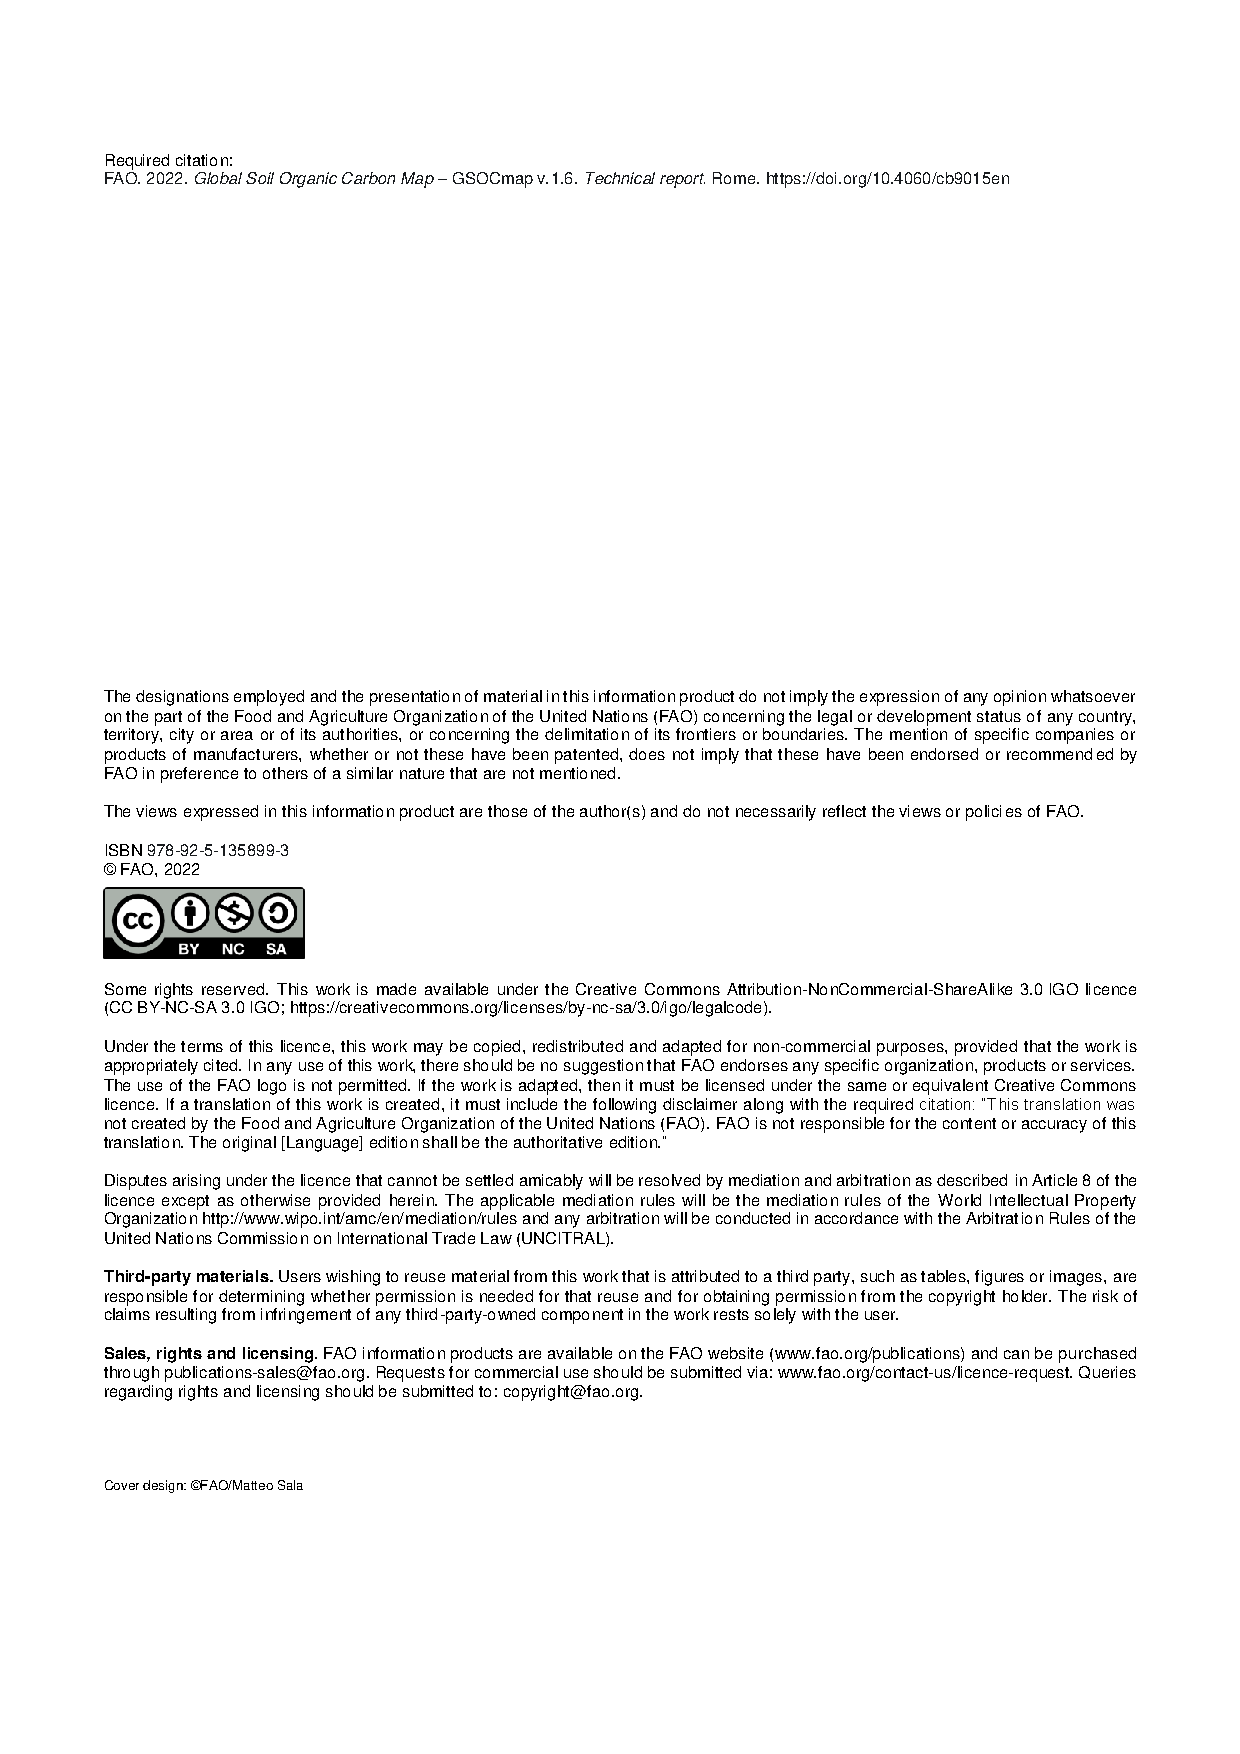
\includepdf{images/CB9015EN_Copyright Disclaimer_v2.pdf}


\frontmatter
\addtocontents{toc}{\protect\hypersetup{hidelinks}}   
\addtocontents{lof}{\protect\hypersetup{hidelinks}}
\addtocontents{lot}{\protect\hypersetup{hidelinks}}
\addtocontents{lot}{\protect\hypersetup{hidelinks}}
\addtocontents{lot}{\protect\hypersetup{hidelinks}}
\tableofcontents
\listoffigures
\listoftables
\nopagebreak[5]


\includegraphics{images/frontcover.jpg}

\hypertarget{licence}{%
\chapter*{Licence}\label{licence}}
\addcontentsline{toc}{chapter}{Licence}

The GSNmap Technical Manual is made available under the Creative Commons Attribution-NonCommercial-ShareAlike 3.0 IGO licence

\href{https://creativecommons.org/licenses/by-nc-sa/3.0/igo/legalcode}{CC BY-NC-SA 3.0 IGO}.

\hypertarget{abbreviations-and-acronyms}{%
\chapter*{Abbreviations and acronyms}\label{abbreviations-and-acronyms}}
\addcontentsline{toc}{chapter}{Abbreviations and acronyms}

\begin{description}
\item[BD]
Bulk density
\item[CEC]
Cation exchange capacity
\item[CRAN]
Comprehensive R archive network
\item[DSM]
Digital soil mapping
\item[GEE]
Google Earth Engine
\item[GSP]
Global Soil Partnership
\item[INSII]
International Network of Soil Information Institutions
\item[ITPS]
Intergovernmental Technical Panel on Soils
\item[ME]
Mean error
\item[MAE]
Mean absolute error
\item[MEC]
Modelling efficiency coefficient
\item[NDVI]
Normalized difference in vegetation index
\item[QA/QC]
Quality assurance/quality check
\item[RMSE]
Root mean squared error
\item[SOC]
Soil organic carbon
\item[SOM]
Soil organic matter
\end{description}

\hypertarget{contributors-and-reviewers}{%
\chapter*{Contributors and reviewers}\label{contributors-and-reviewers}}
\addcontentsline{toc}{chapter}{Contributors and reviewers}

\textbf{International Network of Soil Information Institutions}\\

\textbf{GSNmap working group}

\textbf{Fourth Intergovernmental Technical Panel on Soils}\\

\mainmatter

\hypertarget{presentation}{%
\chapter{Presentation}\label{presentation}}

\hypertarget{background-and-objectives}{%
\section{Background and Objectives}\label{background-and-objectives}}

Soil nutrient availability can affect ecosystem carbon cycling, plant phenology, plant diversity and community composition, plant-herbivore and plant-soil-microbe interactions, as well as the structure of trophic food webs (\protect\hyperlink{ref-vanSundert2020}{Van Sundert \emph{et al.}, 2020}). Thus, the broad range of effects of nutrient availability also affects ecosystem functioning in face of global changes, for instance the response of plants to elevated levels of CO\textsubscript{2} (\protect\hyperlink{ref-vicca2018}{Vicca \emph{et al.}, 2018}).

In the context of agriculture, the availability of nutrients regulates crop productivity and, as a result, influences food production. Nevertheless, ongoing conflicts and the rise in extreme weather events have led to historically high input prices. This trend is now endangering the progress and achievement of Sustainable Development Goal (SDG) 2, which strives to eliminate hunger by 2030. Soil nutrient data, which serves as a cornerstone for informed choices, now faces a critical juncture, essential for steering agricultural practices towards a sustainable future.

To date, around 2.3 billion people are affected by moderate and severe food insecurity (\protect\hyperlink{ref-FAO2022}{FAO and WHO, 2022}). Despite soil nutrient status and availability being vital to the provisioning of ecosystem services, globally-accessible and harmonised datasets on soil nutrient stocks and soil properties that govern nutrient availability are missing.

Therefore, the current global situation requires an increase of food production while preserving natural (soil) resources, lowering greenhouse gas emissions and optimising the use of agricultural inputs such as fertilisers (\protect\hyperlink{ref-eisenstein2020}{Eisenstein, 2020}). Fertiliser prices more than doubled within one year and grain prices increased by around 25 percent (Jan.~2021 - Jan.~2022) (\protect\hyperlink{ref-ifpri2020}{Hebebrand and Laborde, 2022}). With the start of the armed conflict in Ukraine in February 2022, this trend became more pronounced.
Growing food insecurity and rapidly increasing fertiliser prices underscore the urgent need for informed decision-making and optimised soil nutrient management. However, a large data gap exists in regards to soil nutrient stocks and soil properties that govern nutrient availability. Therefore, FAO's Global Soil Partnership (GSP) has launched the Global Soil Nutrient and Nutrient Budget map (GSNmap) initiative in an endeavour to provide harmonised soil nutrient data and information to stakeholders following a country-driven (bottom-up) approach.
Up-to-date soil data on the status and spatial trends of soil nutrients and related soil attributes is key to guide decision makers to close yield gaps, optimize soil nutrient management and protect local natural resources. Therefore, locally-specific information on the status of soil nutrients are needed (\protect\hyperlink{ref-cunningham2013}{Cunningham \emph{et al.}, 2013}). The soil information collected in the GSNmap thereby serves as a cornerstone in delineating priority areas for action and thereby seizes the opportunity to reduce food insecurity, close yield gaps, and reduce environmental costs arising from mismanagement of soil nutrients.

\hypertarget{global-soil-partnership}{%
\section{Global Soil Partnership}\label{global-soil-partnership}}

The Global Soil Partnership (GSP) was established in December 2012 as a mechanism to develop a strong interactive partnership and to enhance collaboration and generate synergies between all stakeholders to raise awareness and protect the world's soil resources. From land users to policymakers, one of the main objectives of GSP is to improve governance and promote sustainable management of soils. Since its creation, GSP has become an important partnership platform where global soil issues are discussed and addressed by multiple stakeholders at different levels.

The mandate of GSP is to improve governance of the planet's limited soil resources in order to guarantee productive agricultural soils for a food-secure world. In addition, it supports other essential soil ecosystem services in accordance with the sovereign right of each Member State over its natural resources. In order to achieve its mandate, GSP addresses six thematic action areas to be implemented in collaboration with its regional soil partnerships (Figure 1).

The area of work on Soil Information and Data (SID) of the GSP builds an enduring and authoritative global system (GloSIS) to monitor and forecast the condition of the Earth's soil resources and produce map products at the global level. The International Network of Soil Information Institutions (INSII) consists of nationally mandated institutions and GSP partners working together to develop GloSIS. These institutions possess the necessary technical expertise to create and exchange specific national soil information and data. Whether they are sub-national or national, regional or global, all institutions have the opportunity to join the INSII network and contribute to the collection and dissemination on the status of soil resources.

\hypertarget{country-driven-approach-and-tasks}{%
\section{Country-driven approach and tasks}\label{country-driven-approach-and-tasks}}

The GSNmap initiative is jointly implemented by the International Network of Soil Information Institutions (INSII) and the GSP Secretariat. The process is country-driven, involving and supporting all GSP members in developing their national GSNmap data products. The GSNmap products are being developed following a two-phase approach:

\begin{itemize}
\tightlist
\item
  Phase I: development of soil nutrient and associated soil property maps;
\item
  Phase II: quantification, analysis, projections of nutrient budgets for croplands.
\end{itemize}

This Technical Manual focuses on the specific methodology to implement Phase I of the GSNmap. It covers the generation of soil property maps for the soil attributes specified in table \ref{tab:overviewprop}. The methodology presented in this document was reviewed and endorsed by INSII and is part of the Country guidelines and technical specifications for global soil nutrient and nutrient budget maps (\protect\hyperlink{ref-FAO2022b}{Food and United Nations, 2022}).

\begin{table}

\caption{\label{tab:overviewprop}Mandatory soil attributes and units of the phase I Global Soil Nutrient and Nutrient Budget Maps}
\centering
\begin{tabular}[t]{lll}
\toprule
Soil property & property id & Unit\\
\midrule
Total N & n\_0\_30 & ppm\\
Available P & p\_0\_30 & ppm\\
CEC & cec\_0\_30 & cmol(c)/kg\\
pH (water) & ph\_0\_30 & /\\
Clay & clay\_0\_30 & \%\\
\addlinespace
Silt & silt\_0\_30 & \%\\
Sand & sand\_0\_30 & \%\\
Soil Organic Carbon & soc\_0\_30 & \%\\
Bulk density & bd\_0\_30 & g/cm3\\
Available K & k\_0\_30 & ppm\\
\bottomrule
\end{tabular}
\end{table}

Depending on national data availability and technical capacities, ad-hoc solutions will be developed by the GSNmap WG to support countries during the national GSNmap production and/or harmonisation phase. Where possible, GSP Secretariat will use publicly available data to gap-fill the areas which are not covered by the national submissions unless the country requests to be left blank on the GSNmap products.

\hypertarget{how-to-use-this-book}{%
\section{How to use this book}\label{how-to-use-this-book}}

The present document is a technical manual on the phase I of the GSNmap initiative. It provides the scientific background on the importance of soil nutrients and guidance on the digital soil mapping techniques to map nutrients and soil properties that govern nutrient availability. It also comprises a compendium with all necessary scripts to generate national GSNmaps. These scripts are described step-by-step in 4 steps that cover soil data preparation (Step 1), covariate download (Step 2), the mapping process itself (Step 3), and the automatic generation of national reports (Step 4). The general workflow is shown in Figure \ref{fig:steps}.

\begin{figure}
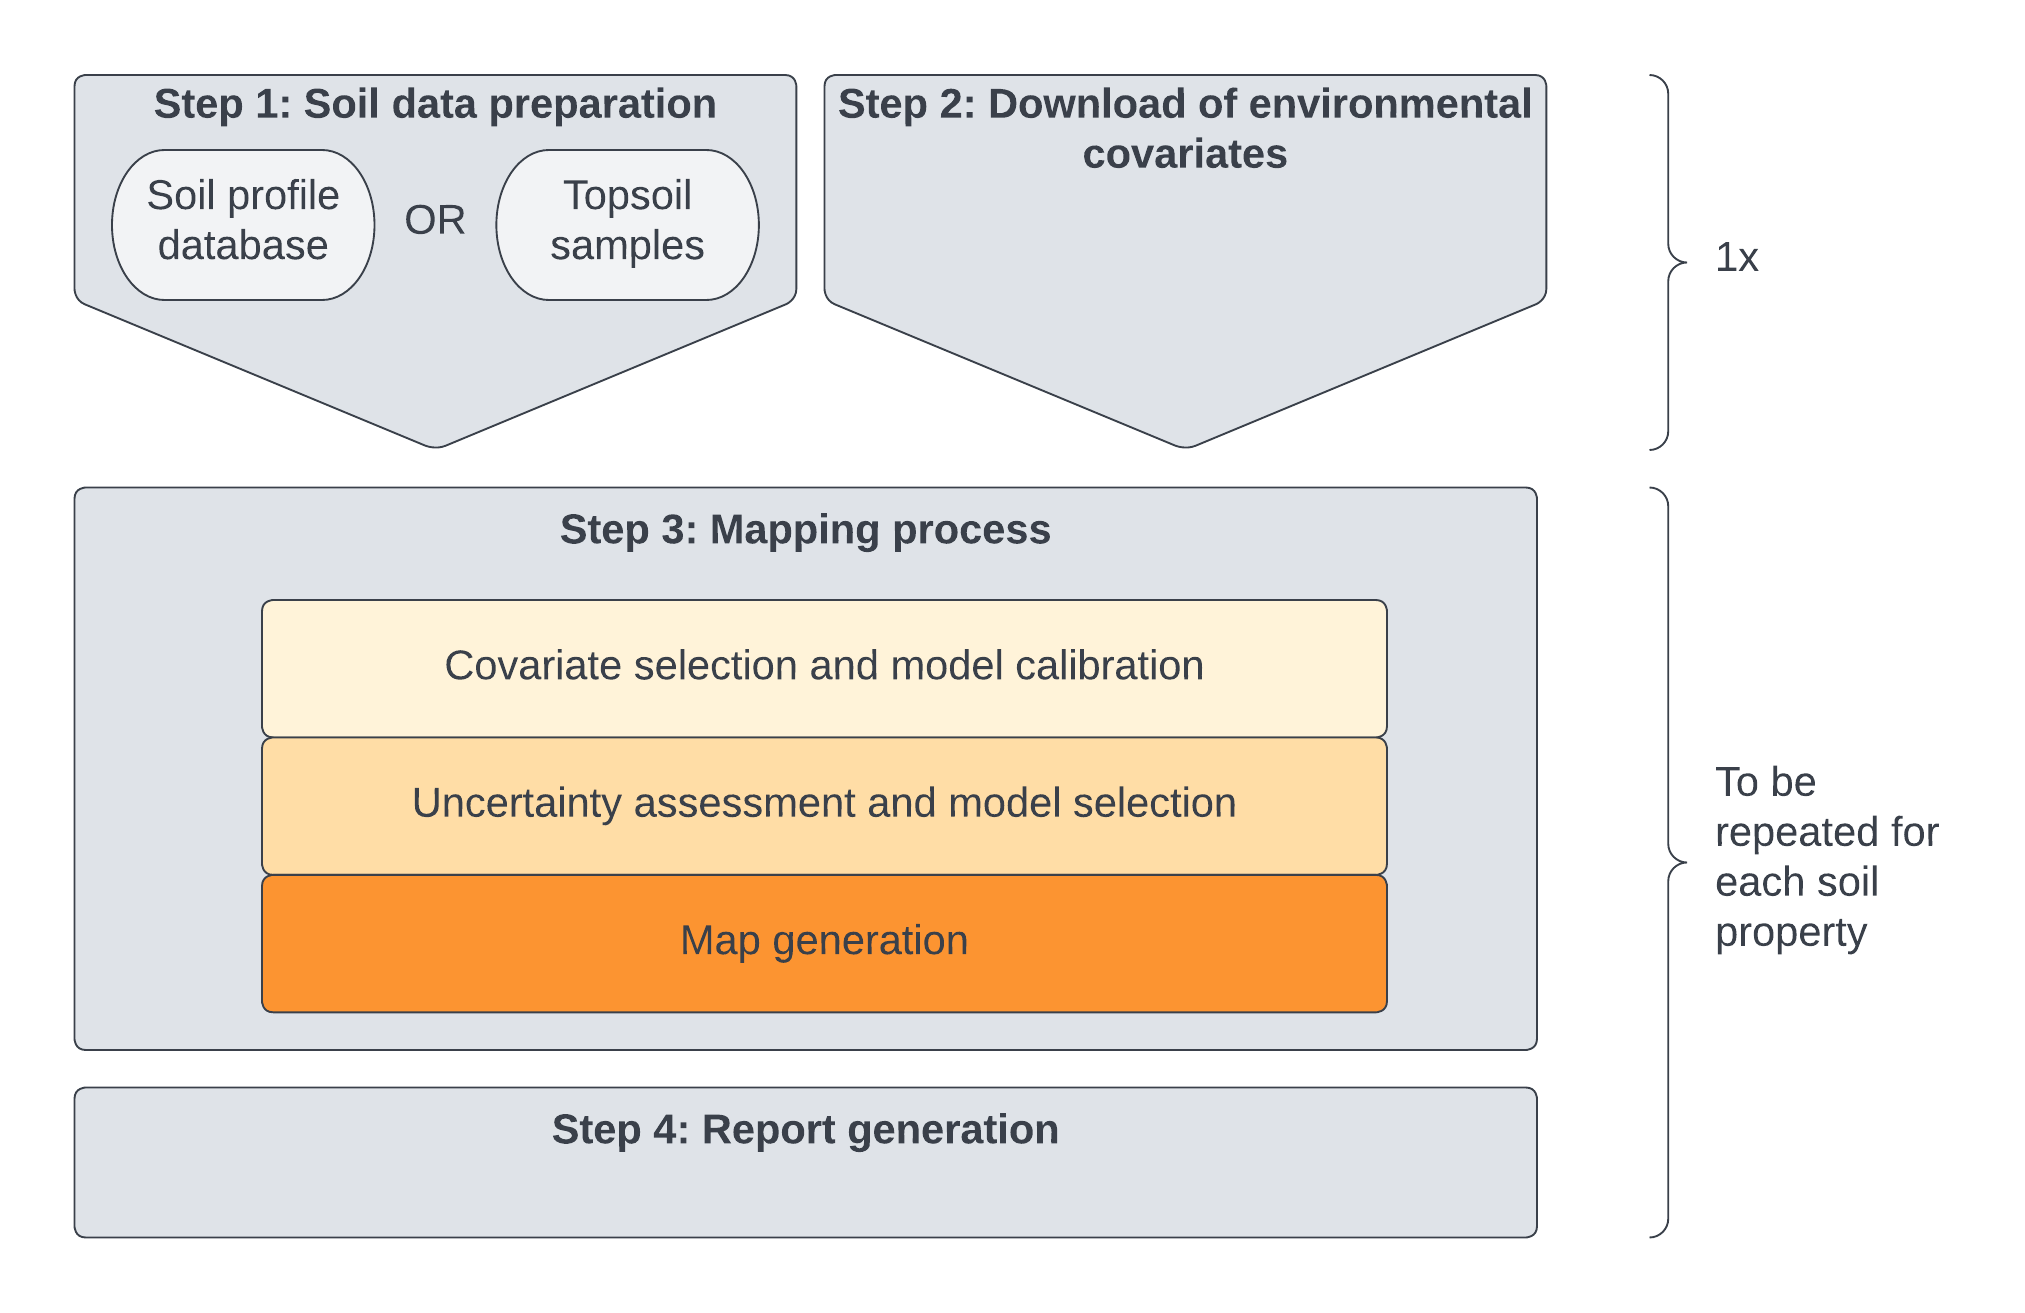
\includegraphics[width=1\linewidth]{images/Manual-Workflow} \caption{Overview of the steps to follow for the GSNmap generation.}\label{fig:steps}
\end{figure}

The chapters are structured as following:

\begin{itemize}
\tightlist
\item
  Chapter 1 provides general information about the GSNmap initiative as well as FAO's Global Soil Partnership (GSP).
\item
  Chapter 2 focuses on the scientific state-of-the-art in terms of soil nutrients and soil nutrient mapping.
\item
  Chapter 3 and 4 introduce the software requirements and the concept of digital soil mapping.
\item
  Chapter 5 to 7 guide the reader through the nutrient mapping exercise of GSNmap Phase I providing step-by-step instructions.
\item
  Chapter 8 explains how the national GSNmaps are reported to the GSP.
\item
  Annex I serves as a repository for the complete scripts needed for the GSNmap.
\item
  Annex II provides alternative step-by-step instructions for the special case of soil data without point coordinates.
\end{itemize}

The GSNmap Technical Manual is structured as a practical document to be used by national experts in the endeavour to employ digital soil mapping techniques to generate national nutrient maps based on a common methodology. The concept of digital soil mapping presented here can however be also used in mapping exercises that focus on other soil properties and is therefore also relevant to scientists and digital soil mappers. The training material and the folders of the technical manual can be downloaded as .zip file here: \url{https://github.com/FAO-GSP/GSNmap-TM/archive/refs/heads/main.zip}. Alternatively, the GitHub repository can be cloned to your local device by using the following link: \url{https://github.com/FAO-GSP/GSNmap-TM.git}.

\hypertarget{training-material}{%
\section{Training material}\label{training-material}}

The train material of this book is located in the \href{https://github.com/FAO-GSP/GSNmap-TM}{GSNmap-TM GitHub repository}. To download the input files and \textbf{R} scripts, clone the repository or click on \href{https://github.com/FAO-GSP/GSNmap-TM/archive/refs/heads/main.zip}{this link}, save the ZIP file and extract its content in a folder, preferable close to the root of your system, such as \texttt{"C:/GIT/"}.

\hypertarget{soil-nutrients}{%
\chapter{Soil Nutrients}\label{soil-nutrients}}

\hypertarget{definition-of-soil-nutrients}{%
\section{Definition of soil nutrients}\label{definition-of-soil-nutrients}}

In theory, soil nutrients are defined as those chemical elements that are \emph{essential} to plant growth (\protect\hyperlink{ref-arnon1939}{Arnon and Stout, 1939}; \protect\hyperlink{ref-vonLiebig1841}{Liebig, 1841}). First, von Liebig (1841) declared nitrogen (N), sulphur (S), phosphorus (P), potassium (K), calcium (Ca), magnesium (Mg), silicon (Si), sodium (Na) and iron (Fe) as being essential. However, these findings lacked experimental research and were based on merely observational studies. Furthermore, if plant uptake is the only criteria for essentiality, the definition disregards the fact that plants also take up innecessary or even toxic elements.
Therefore, stricter criteria such as the one by Arnon and Stout (\protect\hyperlink{ref-arnon1939}{1939}) were defined. They postulated that three criteria need to be met for an \emph{essential mineral nutrients} (\protect\hyperlink{ref-mengel2012}{Mengel and Kirkby, 2012}):
1. Nutrient must be required by plants to complete their life cycle;
2. Nutrient must be irreplaceable; and
3. Nutrient must be involved in the plant metabolism.

Following this defintion to date the following nutrients would be considered essential for higher plants (\protect\hyperlink{ref-mengel2001}{Mengel \emph{et al.}, 2001}): carbon (C), hydrogen (H), oxygen (O), N, P, S, cobalt (Co), K, Ca, Mg, Fe, manganese (Mn), copper (Cu), Si, zinc (Zn), molybdenum (Mo), boron (B), chlorine (Cl), nickel (Ni), Na. However, Co, Si, Ni, and Na are not considered essential for all plants.

Other definitions used biochemical functions for classification purposes (\protect\hyperlink{ref-mengel2001}{Mengel \emph{et al.}, 2001}). Here, four nutrient groups are distinguished:
1. major constituents of organic material (C, H, O, N, S);
2. nutrients that are involved in esterification of alcohol groups (P, B, Si);
3. nutrients that establish an osmotic potential (ions) (K, Na, Ca, Mg, Mn, Cl); and
4. nutrients that enable electron transport (ions or chelates) (Fe, Cu, Zn, Mo).

Still, the most common classification of soil nutrients is based on the absolute quantities of an element that a plant takes up resulting in macro- and micronutrients (\protect\hyperlink{ref-mengel2012}{Mengel and Kirkby, 2012}). Despite being widely used, the definition has several shortcomings as also toxic elements can be taken up in greater quantities (e.g.~Al). Furthermore, the threshold definition between macro- and micronutrients is somewhat arbitrary (\protect\hyperlink{ref-mengel2012}{Mengel and Kirkby, 2012}).
It is important to point out that the discussion on how to accurately define \emph{essential} nutrients is ongoing as recent contribution to the topic show (\protect\hyperlink{ref-brown2022}{Brown, Zhao and Dobermann, 2022}). The generation of the GSNmaps is oriented by the recently published report on the state of the art of soils for nutrition (\protect\hyperlink{ref-symposium2022}{FAO, 2022}) and is shown in Table \ref{tab:nutrients}. It is based on the contribution of each element to the average plant content.

\begin{table}

\caption{\label{tab:nutrients}Classification of major and micronutrients by FAO (2022).}
\centering
\begin{tabular}[t]{ll}
\toprule
Major nutrients & Micronutrients\\
\midrule
N & Fe\\
P & Mn\\
K & Zn\\
Ca & Cu\\
Mg & B\\
\addlinespace
S & Mo\\
 & Cl\\
\bottomrule
\end{tabular}
\end{table}

\hypertarget{soil-properties-governing-nutrient-availability}{%
\section{Soil properties governing nutrient availability}\label{soil-properties-governing-nutrient-availability}}

The uptake of nutrients by plants is regulated in parts by the organism itself as for instance shoot growth is coupled with root growth (\protect\hyperlink{ref-wang2007}{Wang \emph{et al.}, 2007}). Still, soil properties mediate nutrient mobility and conditions at the plant-soil interface. The most important soil properties that determine nutrient availability are physicochemical properties such as soil pH, cation exchange capacity (CEC), soil texture, soil organic matter (SOM) content, and bulk density (BD).
Most nutrients are taken up in their ionized form (\protect\hyperlink{ref-robertson1999}{Robertson \emph{et al.}, 1999}). Therefore, the chemical characterization of the soil solution is key to understand nutrient dynamics and uptake.
Soil pH, as a measure of exchangeable hydrogen protons (H\textsuperscript{+}), is a crucial parameter to determine the acidity of the soil solution that can inhibit or mediate nutrient uptake. For instance, very low pH values of around 4 decreased the uptake of (basic) cations such as Ca or Mg by paddy rice, wheat, corn, common bean and cowpea whereas lower pH values favoured the uptake of Zn, Fe, and Mn. At higher pH values the uptake of cations was enhanced (\protect\hyperlink{ref-fageria2014}{Fageria and Knupp, 2014}).
The CEC, as a measure of exchangeable cations (e.g K\textsuperscript{+}, Mg\textsuperscript{2+}, Ca\textsuperscript{2+}, etc.) available in the soil solution and attached to soil particles is a complementary parameter of nutrient availability in soils (\protect\hyperlink{ref-robertson1999}{Robertson \emph{et al.}, 1999}). The CEC informs on the capacity of soils to retain positively charged nutrients (basic cations) and thus gives information on how strong a soil can buffer subsequent acidification. This retention and buffer capacity is strongly linked to soil texture. High clay contents usually lead to higher CEC and thus higher cation retention. Conversely, sandy textured soils strongly rely on soil organic matter (SOM) content that has high CEC to retain cations.
SOM content further augments aeration of soils due to its low density and provides high specific surface area to retain nutrients.
Finally, BD is key to nutrient availability as it governs facilitates or inhibits root growth and thus nutrient uptake by plants. Due to its impact on soil porosity, BD also governs microbial activity (through aeration) and water infiltration that defines nutrient mobility.

\hypertarget{setting-up-the-software-environment}{%
\chapter{Setting-up the software environment}\label{setting-up-the-software-environment}}

This chapter provides an overview on the software required to map soil nutrients and associated soil properties. The tools are open source and can be downloaded and installed by users following the steps that are described here.

\hypertarget{use-of-r-rstudio-and-r-packages}{%
\section{Use of R, RStudio and R Packages}\label{use-of-r-rstudio-and-r-packages}}

\textbf{R} is a language and environment for statistical computing created in 1992. It provides a wide variety of statistical (e.g.~linear modeling, statistical tests, time-series, classification, clustering, etc.) and graphical methods, and has been constantly extended by an exceptionally active user community.

\hypertarget{obtaining-and-installing-r}{%
\subsection{Obtaining and installing R}\label{obtaining-and-installing-r}}

Installation files and instructions can be downloaded from the Comprehensive R Archive Network (CRAN).

\begin{enumerate}
\def\labelenumi{\arabic{enumi}.}
\tightlist
\item
  Go to the following link \url{https://cran.r-project.org/} to download and install \textbf{R}.
\item
  Pick an installation file for your operational system.
\item
  Choose the ``\emph{base}'' distribution of R (particularly if it is the first time you install \textbf{R}).
\item
  Download the R installation file and open the file on your device.
\item
  Follow the installation instructions.
\end{enumerate}

\hypertarget{obtaining-and-installing-rstudio}{%
\subsection{Obtaining and installing RStudio}\label{obtaining-and-installing-rstudio}}

Beginners will find it very hard to start using \textbf{R} because it has no Graphical User Interface (GUI). There are some GUIs which offer some of the functionality of \textbf{R}. \textbf{RStudio} makes \textbf{R} easier to use. It includes a code editor, debugging and visualization tools. Similar steps need to be followed to install \textbf{RStudio}.

\begin{enumerate}
\def\labelenumi{\arabic{enumi}.}
\tightlist
\item
  Go to \url{https://www.rstudio.com/products/rstudio/download/} to download and install \textbf{RStudio}'s open source edition.
\item
  On the download page, \emph{RStudio Desktop, Open Source License} option should be selected.
\item
  Pick an installation file for your platform.
\item
  Follow the installation instruction on your local device.
\end{enumerate}

\begin{figure}
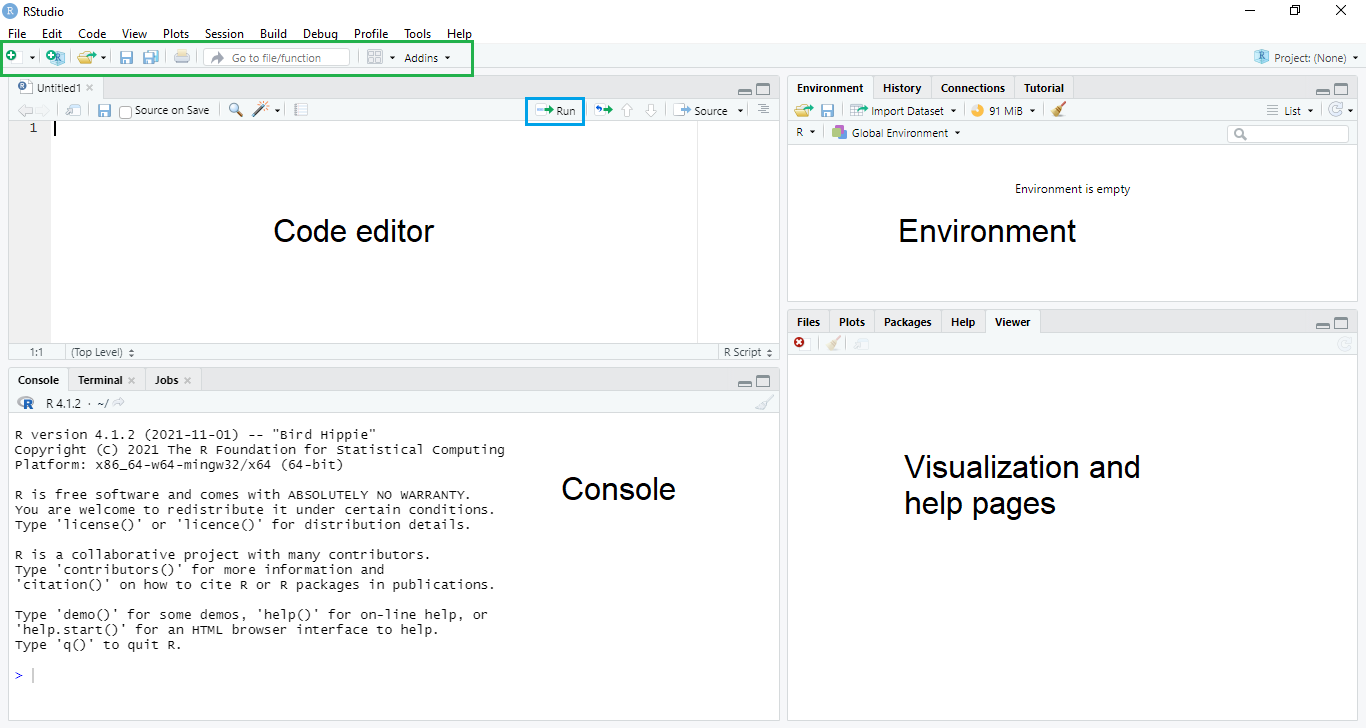
\includegraphics[width=1\linewidth]{images/2_RStudio-interface} \caption{R Studio interface.}\label{fig:Rstudio}
\end{figure}

The \textbf{RStudio} interface is structured by four compartments (see Fig. \ref{fig:Rstudio}). The code editor is located in the upper left. Scripts that contain codes are displayed here. New scripts can be opened by clicking on the left most \emph{New} button in the quick access tool bar (highlighted in green). Lines of code can be executed by clickinig on \emph{Run} (highlighted in blue) or by pressing \emph{ctrl + enter} on your keyboard.
The output of scripts or lines of code that are executed is displayed in the window below the code editor: the console (bottom left). This part of the interface corresponds to the \textbf{R} software that were installed previously.
When working in \textbf{R}, it is central to work with so-called objects (for instance vectors, dataframes or matrices). These objects are saved in the global environment that is displayed in the top right panel.
Finally, the \textbf{R} software offers a broad range of powerful tools for visualisation purposes. Graphs or maps that are generated by scripts/codes, are displayed in the bottom right panel.

\hypertarget{getting-started-with-r}{%
\subsection{Getting started with R}\label{getting-started-with-r}}

\begin{itemize}
\tightlist
\item
  \textbf{R} manuals: \url{http://cran.r-project.org/manuals.html}
\item
  Contributed documentation: \url{http://cran.r-project.org/other-docs.html}
\item
  Quick-\textbf{R}: \url{http://www.statmethods.net/index.html}
\item
  Stackoverflow \textbf{R} community: \url{https://stackoverflow.com/questions/tagged/r}
\end{itemize}

\hypertarget{r-packages}{%
\section{R packages}\label{r-packages}}

When you download \textbf{R}, you get the basic \textbf{R} system which implements the \textbf{R} language. \textbf{R} becomes more useful with the large collection of packages that extend the basic functionality of it. \textbf{R} packages are developed by the \textbf{R} community.

refer to:
* \emph{tidyverse} book (R for data science)
* \emph{caret} (broad range of statistical learning functions)
* \emph{R spatial}: \url{https://rspatial.org/} (R packages for spatial data operations)

The primary source for \textbf{R} packages is \href{https://cran.r-project.org/}{CRAN's} official website, where currently about 12,000 available packages are listed. For spatial applications, various packages are available. You can obtain information about the available packages directly on CRAN with the `available.packages()' function. The function returns a matrix of details corresponding to packages currently available at one or more repositories. An easier way to browse the list of packages is using the \href{https://cran.r-project.org/web/views/}{\emph{Task Views}} link, which groups together packages related to a given topic.

Packages come along with extensive documentation that is very helpful to understand and solve error messages. To access information on functions or packages, type ``?{[}Package or Function name{]}'' in the console. The information on the package and/or function can then be accessed in the bottom right panel under ``Help'' (see Fig. \ref{fig:Rstudio}). In addition to that, the \emph{R documentation} website (\url{https://www.rdocumentation.org/}) provides more extensive help and gives clear overviews on all functions comprised in a certain package.

\hypertarget{gee---google-earth-engine}{%
\section{GEE - google earth engine}\label{gee---google-earth-engine}}

Google earth engine (GEE) provides a large range of remote sensing datasets for users. It allows to use the GEE code editor to run computations using the google servers. The high computational power of these servers enables users with limited computational caapacities to run complex calculations.
A user account must be created to use the code editor. This step can take some time. Once the account is validated, scripts can be written in the code editor using the Javascript language. An extensive array of instructions and guides are available on the platform. Alternatively, the Python language can be used to interact with the data.

The code editor interface is structured by three panels and a map viewer (see Fig. \ref{fig:GEE}). The left panel is structured in ``Scripts'', ``Docs'', and ``Assets''. Under ``Scripts'' users can organize and save the scripts they wrote for specific purposes. ``Docs'' provides further information on so-called ``server-side'' functions that can be used to manipulate the data. Finally, in ``Assets'' users can upload own spatial data in common formats such as shapefiles (.shp) or raster files (.tif).
The middle panel contains the scripts that can be run by clicking on the ``Run'' button.
The right panel is composed of three functionalities. The ``Inspector'' provides basic information on a pixel of a layer displayed in the map below. The information consists of longitude, latitude, and - if layers are loaded - values of the pixel. The ``Console'' is the place where certain commands expressed in the code are shown. The most common expressions shown here are print() commands or figures derived from the loaded data. Finally, the ``Tasks'' button shows all tasks that were formulated in the code/script and are to be submitted to the server for computation. Once a task is submitted, the user has to click on the ``Run'' button appearing in the ``Tasks'' section to submit the task to the server.
In addition to that, the data catalog can be accessed via the search bar on the top of the page. Here, key information on the available datasets, origin, resolution and related publications can be found.

\begin{figure}
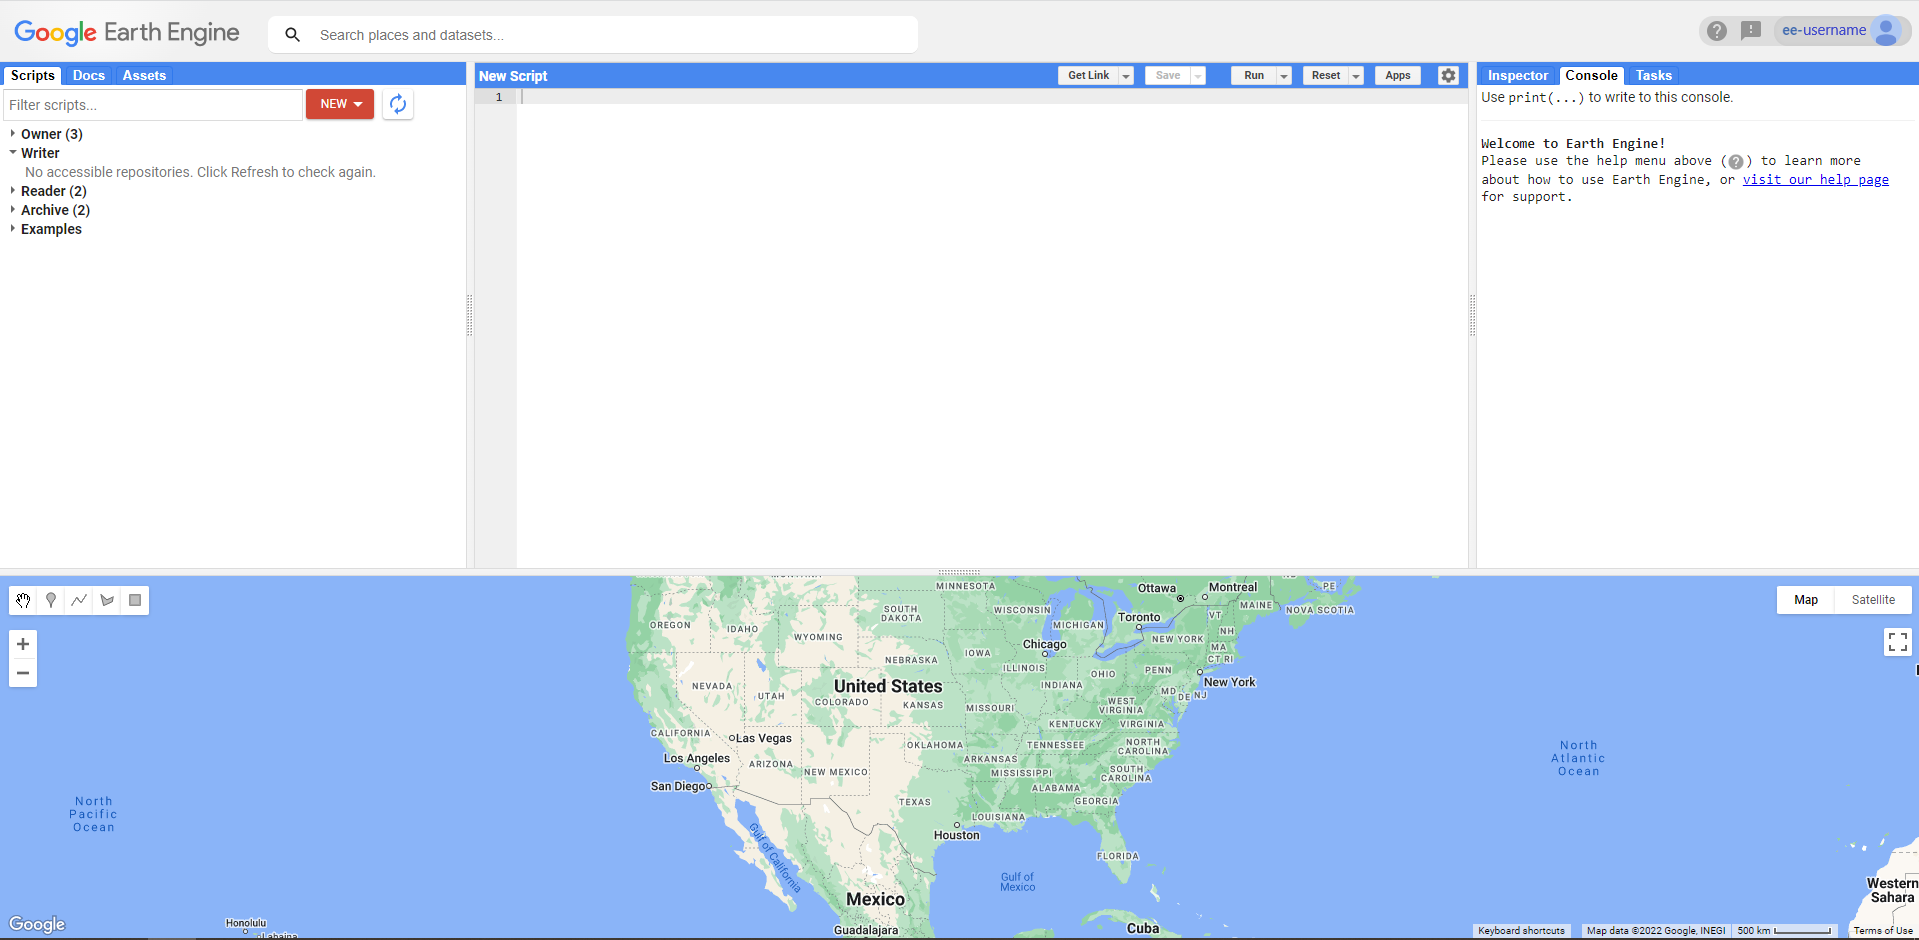
\includegraphics[width=1\linewidth]{images/2.1_GEE_codeeditor} \caption{Google Earth Engine code editor.}\label{fig:GEE2}
\end{figure}

\hypertarget{digital-soil-mapping}{%
\chapter{Digital Soil Mapping}\label{digital-soil-mapping}}

\hypertarget{principles}{%
\section{Principles}\label{principles}}

Digital soil mapping (DSM) is a methodological framework to create soil attribute maps on the basis of the quantitative relationships between spatial soil databases and environmental covariates. The quantitative relations can be modelled by different statistical approaches, most of them considered machine learning techniques. Environmental covariates are spatially explicit proxies of soil-forming factors that are employed as predictors of the geographical distribution of soil properties. The methodology has evolved from the theories of soil genesis developed by Dokuchaev (\protect\hyperlink{ref-Dokuchaev1883}{1883}) in his work the Russian Chernozems, which later were formalised by Jenny (\protect\hyperlink{ref-Jenny1941}{1941}) with the equation of the soil-forming factors. The conceptual equation of soil-forming factors has been updated by McBratney, Santos and Minasny (\protect\hyperlink{ref-McBratney2003}{2003}) as follow:

\begin{equation} 
  S = f\left(s,c,o,r,p,a,n\right)
  \label{eq:scorpan}
\end{equation}

Where \(S\) is the soil classes or attributes (to be modelled) as a function of ``\(s\)'' as other soil properties, ``\(c\)'' as climatic properties, ``\(o\)'' as organisms, including land cover and human activity, ``\(r\)'' as terrain attributes, ``\(p\)'' as parent material, ``\(a\)'' as soil age, and ``\(n\)'' as the geographic position.

\hypertarget{covariates}{%
\section{Covariates}\label{covariates}}

Covariates are geospatially referenced parameters that constitute pivotal determinants within the domain of digital soil mapping. Covariates encapsulate the underlying drivers shaping soil variability, aiding in the prediction of soil properties across landscapes. These variables consist of a diverse range of factors, including topography, vegetation, climate variables, and land use information among others. Careful selection of relevant covariates is essential, as their choice directly impacts the accuracy of soil property predictions.

\hypertarget{machine-learning-techniques}{%
\section{Machine learning techniques}\label{machine-learning-techniques}}

A broad range of modelling approaches exist in order to establish quantitative relationships between environmental covariates and the target soil properties to be mapped.
Traditionally, multiple linear regression models can be used to quantify the relationships which continues to be the most applied mapping method to map for instance soil organic carbon (\protect\hyperlink{ref-lamichhane2019}{Lamichhane, Kumar and Wilson, 2019}). In addition to that, regression Kriging methods combine linear regressions and an stochastic interpolation of the regression residuals based on their spatial autocorrelation (\protect\hyperlink{ref-yigini2018}{Yigini \emph{et al.}, 2018}).
However, machine learning algorithms with more flexible assumptions, i.e.~non-linear relationships, have become more and more popular as the mapping performance was substantially improved and the versatility of the algorithms can be detect more complex relationships.
Among the most commonly used non-linear machine learning models is random forest (\protect\hyperlink{ref-Breiman2001}{Breiman, 2001}). The random forest algorithm splits a dataset into subsets and uses a random selection of covariates (predictors) to identify homogeneous groups. The procedure of classifying is repeated many times and in the end the prediction is averaged. Traditional random forests output the mean prediction from the random trees. Quantile regression forests (QRF) is an extension of random forests developed by Nicolai Meinshausen (\protect\hyperlink{ref-Meinshausen2006}{Meinshausen, 2006}) that provides non-parametric estimates of the median predicted value as well as prediction quantiles. The benefit of QRF is the ability to predict not only the mean of the prediction but also to provide more information on the uncertainty and probability distribution.

\hypertarget{mapping-of-soil-nutrients-and-associated-soil-attributes}{%
\section{Mapping of soil nutrients and associated soil attributes}\label{mapping-of-soil-nutrients-and-associated-soil-attributes}}

DSM has been used to produce maps of soil nutrients at regional to continental scales. For instance, Hengl \emph{et al.} (\protect\hyperlink{ref-Hengl2017}{2017}) predicted 15 soil nutrients at a 250 m resolution in Africa using a random forest model (\protect\hyperlink{ref-wright2016}{Wright, Ziegler and König, 2016}). The soil nutrient observations were collected for topsoils at locations that were unevenly distributed over the continent and a set of spatially-explicit environmental covariates including soil properties. In 2021, the map resolution was increased to 30 x 30 m by using additional soil samples (\protect\hyperlink{ref-hengl2021}{Hengl \emph{et al.}, 2021}).
In Europe maps of chemical soil properties, including macronutrients like potassium and phosphorus, were mapped based on a gaussian process regression using the LUCAS soil database (\protect\hyperlink{ref-ballabio2019}{Ballabio \emph{et al.}, 2019}).
Global efforts to map soil nutrients in a harmonised way are hampered by the limited availability of appropriate soil data. The country-driven approach of the GSP can potentially overcome this limitation by fostering and leveraging national expertise. To implement the GSP's country-driven global mapping exercise, this Technical Manual provides step-by-step guidelines to map soil nutrients and associated properties using georeferenced soil observations following a digital soil mapping approach using the quantile regression forest algorithm (Figure \ref{fig:workflow1}).

\begin{figure}
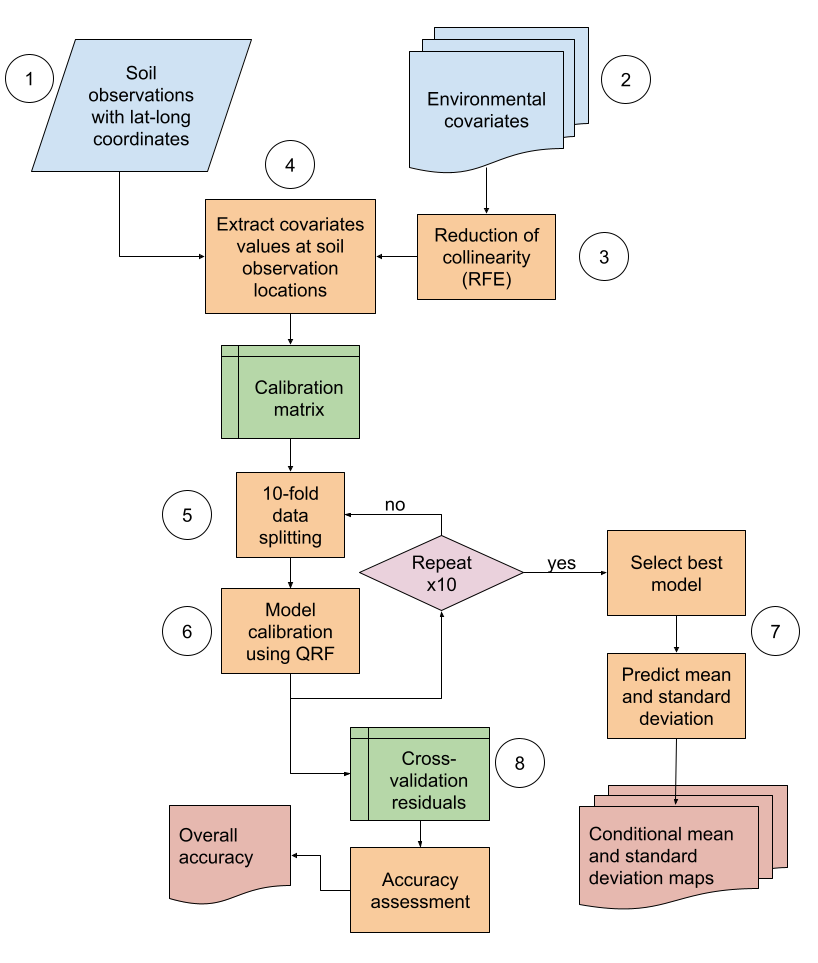
\includegraphics[width=1\linewidth]{images/workflow_lat_long_data} \caption{Digital soil mapping approach for the GSNmap Phase I. Circles are the steps.}\label{fig:workflow1}
\end{figure}

\hypertarget{the-training-dataset-and-basic-computations-in-r}{%
\chapter{\texorpdfstring{The training dataset and basic computations in \textbf{R}}{The training dataset and basic computations in R}}\label{the-training-dataset-and-basic-computations-in-r}}

In this chapter, the datasets used in this technical manual are presented. They were adapted for educational purposes by the GSP Secretariat.
The tutorial provided in this chapter is for demonstration purposes and is meant for users with no prior experience in \textbf{R}.
Thus, the instructions also serve as a continuation of the basic introduction to the functioning of \textbf{R} and \emph{RStudio} given in \href{https://fao-gsp.github.io/GSNmap-TM/setting-up-the-software-environment.html\#use-of-r-rstudio-and-r-packages}{Chapter 3}.

Instructions are given on how to:

\begin{enumerate}
\def\labelenumi{\arabic{enumi}.}
\tightlist
\item
  Generate user-defined variables,
\item
  Set the working directory and load necessary packages,
\item
  Import national data to \emph{RStudio}
\end{enumerate}

Users with prior experience may skip this chapter and go directly to Chapters 6 to 9 which cover all the necessary steps from data preparation to mapping and reporting.

\hypertarget{study-area-and-training-material}{%
\section{Study area and training material}\label{study-area-and-training-material}}

The study area is located in the southeast of the Pampas Region, in Argentina, from the foothills of the Ventania and Tandilia hill systems, until the southern coasts of the Buenos Aires Province.
To illustrate the different processes of this Technical Manual, we use three datasets from this region:

\begin{itemize}
\tightlist
\item
  Georeferenced topsoil data

  \begin{itemize}
  \tightlist
  \item
    Chemical soil properties
  \item
    Physical soil properties
  \end{itemize}
\item
  Soil profile data
\end{itemize}

\hypertarget{georeferenced-topsoil-data}{%
\subsection{Georeferenced topsoil data}\label{georeferenced-topsoil-data}}

These data were collected in 2011 by the National Institute of Agriculture Technology and Faculty of Agricultural Science of the National University of Mar del Plata (Unidad Integrada INTA-FCA) to map the status of soil nutrients in the Argentinian Pampas (\protect\hyperlink{ref-sainz2019}{Sainz Rozas \emph{et al.}, 2019}). The modified dataset is derived from a subset of 118 locations and covers the target depth of 0-30 cm. It is structured in two different spreadsheets that contain \emph{soil chemical properties} (soil\_chem\_data030.csv) and \emph{soil physical properties} (soil\_phys\_data030.csv). All datasets are located in the \texttt{01-Data} folder in the training material \texttt{Digital-Soil-Mapping} folder.
The soil chemical properties spreadsheet provides data from laboratories with point coordinates (lat/long) together with data on available Phosphorus (p\_bray, in ppm), available Potassium (k, in ppm), and total nitrogen (tn, in Percent) (see Table \ref{tab:table2}).

\begin{table}

\caption{\label{tab:table2}Dataset with coordinates for chemical soil properties.}
\centering
\begin{tabular}[t]{lrrrrr}
\toprule
LabID & x & y & p\_bray & k & tn\\
\midrule
51 & -61.51282 & -37.37646 & 20.40 & 852.17 & 0.22\\
60 & -57.84725 & -37.85136 & 10.52 & 769.55 & 0.30\\
64 & -58.87620 & -38.54000 & 15.87 & 992.41 & 0.27\\
67 & -60.30394 & -38.45300 & 20.85 & 740.24 & 0.18\\
68 & -60.39772 & -38.51567 & 13.54 & 724.77 & 0.17\\
\addlinespace
69 & -60.41442 & -38.52914 & 46.17 & 699.03 & 0.13\\
74 & -60.00556 & -38.76500 & 20.94 & 518.58 & 0.23\\
75 & -60.10750 & -38.76472 & 26.82 & 450.17 & 0.24\\
77 & -60.17139 & -38.79278 & 22.56 & 858.80 & 0.19\\
78 & -60.03111 & -38.74611 & 20.09 & 662.91 & 0.20\\
\bottomrule
\multicolumn{6}{l}{\rule{0pt}{1em}Only the ten first rows are shown.}\\
\end{tabular}
\end{table}

The spreadsheet with soil physical data contains data on soil texture for clay (clay\_0\_30, in g/kg), silt (silt\_0\_30, in g/kg), and sand (sand\_0\_30, in g/kg) (see Table \ref{tab:table22}).

\begin{table}

\caption{\label{tab:table22}Dataset with coordinates for physical soil properties.}
\centering
\begin{tabular}[t]{rrrrrr}
\toprule
ProfID & x & y & clay\_0\_30 & sand\_0\_30 & silt\_0\_30\\
\midrule
154 & -58.67430 & -38.20796 & 259.79 & 410 & 330.21\\
197 & -60.45918 & -38.36285 & 251.05 & 400 & 348.95\\
262 & -58.86694 & -38.42194 & 213.04 & 480 & 306.96\\
2702 & -58.02222 & -37.82167 & 259.71 & 430 & 310.29\\
2706 & -57.91861 & -37.95444 & 265.08 & 400 & 334.92\\
\addlinespace
2709 & -60.47222 & -36.67778 & 323.92 & 310 & 366.08\\
2710 & -60.22856 & -36.69115 & 274.30 & 240 & 485.70\\
2711 & -60.45076 & -36.84394 & 234.67 & 540 & 225.33\\
2712 & -60.42631 & -36.94468 & 293.42 & 310 & 396.58\\
2714 & -59.27717 & -36.95655 & 262.34 & 460 & 277.66\\
\bottomrule
\multicolumn{6}{l}{\rule{0pt}{1em}Only the ten first rows are shown.}\\
\end{tabular}
\end{table}

The distribution of points is shown in the following map for available Phosphorus values as points. This dataset is used in \href{https://fao-gsp.github.io/GSNmap-TM/step-3-mapping-continuous-soil-properties.html}{Chapter 8} for mapping.

\begin{Shaded}
\begin{Highlighting}[]
\FunctionTok{library}\NormalTok{(tidyverse)}
\FunctionTok{library}\NormalTok{(sf)}
\FunctionTok{library}\NormalTok{(mapview)}

\FunctionTok{mapviewOptions}\NormalTok{(}\AttributeTok{fgb =} \ConstantTok{FALSE}\NormalTok{)}
\NormalTok{data }\OtherTok{\textless{}{-}} \FunctionTok{read\_csv}\NormalTok{(}\StringTok{"Digital{-}Soil{-}Mapping/01{-}Data/soil\_chem\_data030.csv"}\NormalTok{)}
\NormalTok{s }\OtherTok{\textless{}{-}} \FunctionTok{st\_as\_sf}\NormalTok{(data, }\AttributeTok{coords =} \FunctionTok{c}\NormalTok{(}\StringTok{"x"}\NormalTok{, }\StringTok{"y"}\NormalTok{), }\AttributeTok{crs =} \DecValTok{4326}\NormalTok{)}
\FunctionTok{mapview}\NormalTok{(s, }\AttributeTok{zcol =} \StringTok{"p\_bray"}\NormalTok{, }\AttributeTok{cex =} \FloatTok{2.5}\NormalTok{, }\AttributeTok{lwd =} \DecValTok{0}\NormalTok{)}
\end{Highlighting}
\end{Shaded}

\hypertarget{soil-profile-data}{%
\subsection{Soil profile data}\label{soil-profile-data}}

Finally, the third dataset belongs to the Soil Information System of Argentina (\href{http://sisinta.inta.gob.ar/}{SISINTA}, Olmedo, Rodriguez and Angelini (\protect\hyperlink{ref-Olmedo2017}{2017})) which contains soil profiles collected from the sixties to recently years for soil survey purposes. The data can be fetched using the package \href{https://github.com/INTA-Suelos/SISINTAR\#readme}{SISINTAR}. Table \ref{tab:table4} shows a subset of the data, and the map presents the distribution of soil profiles for the study area. Soil profile data consists of measurements of soil organic carbon (soc, in Percent), soil pH (ph\_h2o), available Potassium (k), bulk density (bd, in g/cm\textsuperscript{3}), cation exchange capacity (cec, in cmol\textsubscript{c}/100g). This dataset is used in this chapter to illustrate the preprocessing steps required for data that come from soil profiles.

\begin{table}

\caption{\label{tab:table4}Soil profile dataset.}
\centering
\begin{tabular}[t]{rrrrrrrrrr}
\toprule
id\_prof & id\_hor & x & y & top & bottom & ph\_h2o & k & soc & bd\\
\midrule
51 & 28706 & -60.35188 & -38.80600 & 0 & 15 & 6 & 1.5 & 2.6 & NA\\
51 & 28707 & -60.35188 & -38.80600 & 15 & 25 & 6 & 1.7 & 2.5 & NA\\
51 & 28708 & -60.35188 & -38.80600 & 25 & 52 & 6 & 0.8 & 1.3 & NA\\
51 & 28709 & -60.35188 & -38.80600 & 52 & 57 & NA & NA & NA & NA\\
154 & 28425 & -58.67430 & -38.20796 & 0 & 14 & 6 & 2.2 & 3.6 & NA\\
\addlinespace
154 & 28426 & -58.67430 & -38.20796 & 14 & 26 & 6 & 1.9 & 2.8 & NA\\
154 & 28427 & -58.67430 & -38.20796 & 26 & 44 & 6 & 2.5 & 1.1 & NA\\
154 & 28428 & -58.67430 & -38.20796 & 44 & 56 & 7 & 2.2 & 0.5 & NA\\
154 & 28429 & -58.67430 & -38.20796 & 56 & 105 & 6 & 1.8 & 0.2 & NA\\
197 & 28588 & -60.45918 & -38.36285 & 0 & 13 & 6 & 2.8 & 3.4 & NA\\
\bottomrule
\multicolumn{10}{l}{\rule{0pt}{1em}Only ten rows are shown.}\\
\end{tabular}
\end{table}

\begin{Shaded}
\begin{Highlighting}[]
\FunctionTok{library}\NormalTok{(tidyverse)}
\FunctionTok{library}\NormalTok{(sf)}
\FunctionTok{library}\NormalTok{(mapview)}
\FunctionTok{mapviewOptions}\NormalTok{(}\AttributeTok{fgb =} \ConstantTok{FALSE}\NormalTok{)}
\NormalTok{data }\OtherTok{\textless{}{-}} \FunctionTok{read\_csv}\NormalTok{(}\StringTok{"Digital{-}Soil{-}Mapping/01{-}Data/soil\_profile\_data.csv"}\NormalTok{)}
\NormalTok{s }\OtherTok{\textless{}{-}}\NormalTok{ data }\SpecialCharTok{\%\textgreater{}\%} \FunctionTok{filter}\NormalTok{(top}\SpecialCharTok{==}\DecValTok{0}\NormalTok{)}
\NormalTok{s }\OtherTok{\textless{}{-}} \FunctionTok{st\_as\_sf}\NormalTok{(s, }\AttributeTok{coords =} \FunctionTok{c}\NormalTok{(}\StringTok{"x"}\NormalTok{, }\StringTok{"y"}\NormalTok{), }\AttributeTok{crs =} \DecValTok{4326}\NormalTok{)}
\FunctionTok{mapview}\NormalTok{(s, }\AttributeTok{zcol =} \StringTok{"k"}\NormalTok{, }\AttributeTok{cex =} \FloatTok{2.5}\NormalTok{, }\AttributeTok{lwd =} \DecValTok{0}\NormalTok{)}
\end{Highlighting}
\end{Shaded}

\hypertarget{preproc}{%
\section{Format requirements of soil data}\label{preproc}}

Soil data generally consists of measurements at a specific geographical location, time and soil depth. Therefore, it is necessary to arrange the data following the format shown in Table \ref{tab:data1}.

\begin{table}

\caption{\label{tab:data1}Example format of a database.}
\centering
\begin{threeparttable}
\fontsize{5}{7}\selectfont
\begin{tabular}[t]{rlrrrrrrrrrrrr}
\toprule
Profile ID & Horizon ID & Lat & Long & Year & Top & Bottom & cec & ph & clay & silt & sand & soc & bd\\
\midrule
1 & 1\_1 & 12.12346 & 1.123456 & 2018 & 0 & 20 & 15 & 6.5 & 35 & 58 & 7 & 3.4 & 1.31\\
1 & 1\_2 & 12.12346 & 1.123456 & 2018 & 20 & 40 & 19 & 7.1 & 42 & 48 & 10 & 2.1 & 1.32\\
2 & 2\_1 & 23.12346 & 2.123456 & 2019 & 0 & 30 & 14 & 5.5 & 12 & 53 & 35 & 2.9 & 1.39\\
\bottomrule
\end{tabular}
\begin{tablenotes}
\item \textit{Note: } 
\item Profile ID = unique profile identifier, Horizon ID = unique layer identifier, Lat = latitude in decimal degrees, Long = longitude in decimal degrees, Year = sampling year, Top = upper limit of the layer in cm, Bottom = lower limit of the layer in cm, cec = Cation Exchange Capacity (cmol\_c/kg), ph = pH in water, clay = Clay (g/100g soil), silt = Silt (g/100g soil), sand = Sand ((g/100g soil), soc = Soil Organic Carbon (g/100g soil), bd = Bulk Density (g/cm3).
\end{tablenotes}
\end{threeparttable}
\end{table}

\hypertarget{pre-processing-steps}{%
\section{Pre-processing steps}\label{pre-processing-steps}}

Soil data is often arranged in a different way which requires specific pre-processing steps to reach the format. On the way towards a formatted database, common issues such as, arranging the data format, fixing soil horizon depth consistency, detecting unusual soil property measurements, can be solved. Here, common issues and examples are given on how to carry out some basic data handling steps in \emph{RStudio}.

\hypertarget{set-the-scene-set-working-directory-packages-load-data}{%
\subsection{Set the scene (set working directory, packages, load data)}\label{set-the-scene-set-working-directory-packages-load-data}}

Let's open \emph{RStudio}. Whenever starting to work on a project or task, it is necessary to set the \emph{working directory} (WD). The WD is the folder path that is used by \textbf{R} to save the output, for instance a plot or a table that was generated while working in \textbf{R}. Thus, the WD is central since it dictates where the files and calculations can be found afterwards. As it is so important, there are multiple ways of setting the WD.
One option is to right click on `Session' menu \textgreater{} `Set working directory \ldots{}' and select either `To Source File Location' (then the WD corresponds to the file path where the Script is saved to) or `Choose Directory\ldots{}'. Then, the user can browse to the folder that should be the WD.

In this manual we propose an alternative way that allows for more customization and flexibility since sometimes multiple WDs are needed to for instance save the final map in a different folder than the covariates. Since the file paths differ depending on where you stored the file on your computer, it is crucial to identify the correct file path. This can be done by accessing the \emph{file explorer}. There you can browse to your training material folder and then right-click on the bar highlighted in red in the Figure \ref{fig:explorer}.

\begin{figure}
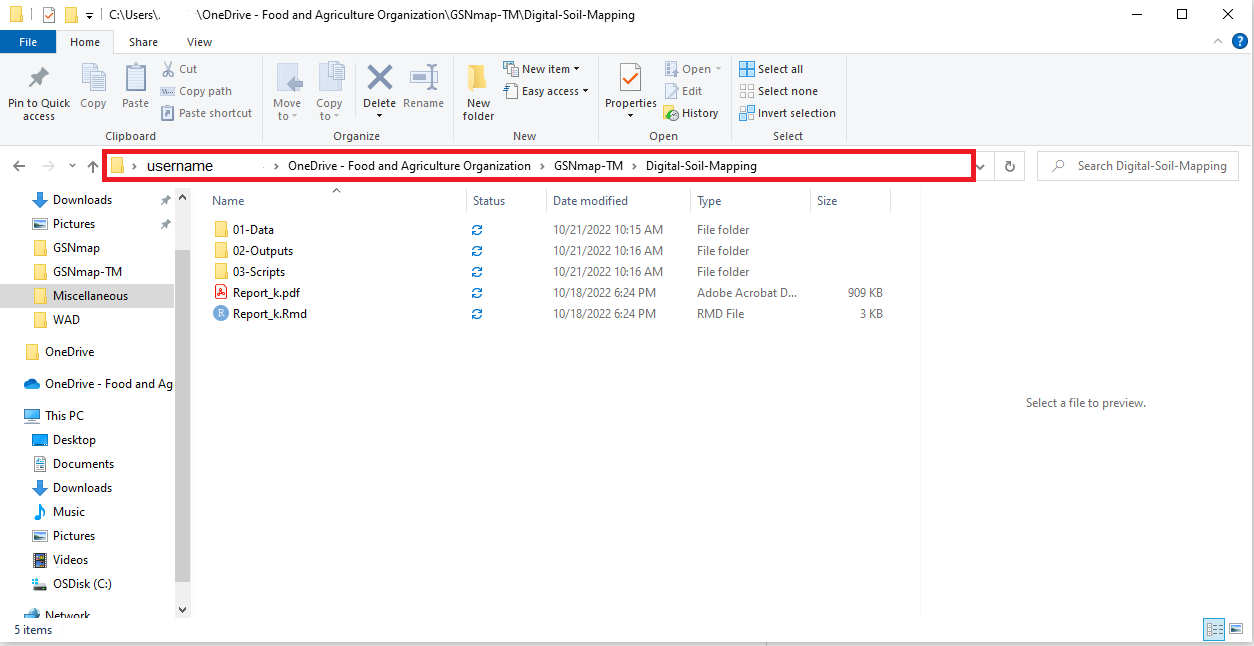
\includegraphics[width=1\linewidth]{images/file-explorer} \caption{Get file path from file explorer.}\label{fig:explorer}
\end{figure}

The file path will appear with the following format: \texttt{C:\textbackslash{}Users\textbackslash{}GSNmap-TM\textbackslash{}Digital-Soil-Mapping}. In order to enable \textbf{R} to read this as file path, it is necessary to replace the \texttt{\textbackslash{}} by \texttt{/}. The resulting file path should look similar to this one: \texttt{C:/Users/GSNmap-TM/Digital-Soil-Mapping}. Once this is done, we can assign the file path that represents the WD file path to an \textbf{R} object. This is done by defining a character value (in this case the file path) on the right side of the arrow (\texttt{\textless{}-}) and name the \textbf{R} object on the left side (wd) (see code). Once this is done we use the function \texttt{setwd()} to set the WD to the file path that is specified in the object \texttt{wd}.

\begin{Shaded}
\begin{Highlighting}[]
\CommentTok{\# 0 {-} User{-}defined variables ===================================================}
\NormalTok{wd }\OtherTok{\textless{}{-}} \StringTok{\textquotesingle{}C:/Users/hp/Documents/GitHub/Digital{-}Soil{-}Mapping\textquotesingle{}}
\CommentTok{\#wd \textless{}{-} "C:/GIT/Digital{-}Soil{-}Mapping"}

\CommentTok{\# 1 {-} Set working directory and load necessary packages ========================}
\FunctionTok{setwd}\NormalTok{(wd) }\CommentTok{\# change the path accordingly}
\end{Highlighting}
\end{Shaded}

An alternative and more automatic approach for setting the working directory makes use of the rstudioapi package, which provides functions for interacting with RStudio's API (Application Programming Interface). The code below first sets the working directory to the directory containing the active document (in this case the script). Then, the second line of code it changes the working directory to the parent directory using the ``..'' specification.

\begin{Shaded}
\begin{Highlighting}[]
\CommentTok{\#Set the working directory automatically using rstudioapi }
\CommentTok{\# It is important to note that the directory is set to the folder containing the script}
\FunctionTok{setwd}\NormalTok{(}\FunctionTok{dirname}\NormalTok{(rstudioapi}\SpecialCharTok{::}\FunctionTok{getActiveDocumentContext}\NormalTok{()}\SpecialCharTok{$}\NormalTok{path))}
\CommentTok{\# The ".." is used to go up a directory (in this case our project folder)}
\FunctionTok{setwd}\NormalTok{(}\StringTok{".."}\NormalTok{)}
\end{Highlighting}
\end{Shaded}

Next to in-built base R functions, there is a vast amount of so-called packages that extend the functionalities of \textbf{R} and allow the use of \textbf{R} for a broad range of purposes. For data handling and management, the \texttt{tidyverse} package and its dependencies offer a great help. To load packages into the \emph{RStudio} session, the \texttt{library} function is used. However, if the package is not installed, it is necessary to use the \texttt{install.packages} function first.

\begin{Shaded}
\begin{Highlighting}[]
\CommentTok{\#install.packages(tidyverse)}
\FunctionTok{library}\NormalTok{(readxl)}
\FunctionTok{library}\NormalTok{(tidyverse)}
\FunctionTok{library}\NormalTok{(dplyr)}

\CommentTok{\# load in data}
\NormalTok{data }\OtherTok{\textless{}{-}} \FunctionTok{read\_csv}\NormalTok{(}\StringTok{"Digital{-}Soil{-}Mapping/01{-}Data/soil\_chem\_data030.csv"}\NormalTok{)}
\end{Highlighting}
\end{Shaded}

\begin{verbatim}
## Rows: 119 Columns: 6
## -- Column specification ----------------------------------
## Delimiter: ","
## chr (1): LabID
## dbl (5): x, y, p_bray, k, tn
## 
## i Use `spec()` to retrieve the full column specification for this data.
## i Specify the column types or set `show_col_types = FALSE` to quiet this message.
\end{verbatim}

\begin{Shaded}
\begin{Highlighting}[]
\FunctionTok{head}\NormalTok{(data)}
\end{Highlighting}
\end{Shaded}

\begin{verbatim}
## # A tibble: 6 x 6
##   LabID     x     y p_bray     k    tn
##   <chr> <dbl> <dbl>  <dbl> <dbl> <dbl>
## 1 51    -61.5 -37.4   20.4  852. 0.225
## 2 60    -57.8 -37.9   10.5  770. 0.301
## 3 64    -58.9 -38.5   15.9  992. 0.266
## 4 67    -60.3 -38.5   20.8  740. 0.179
## 5 68    -60.4 -38.5   13.5  725. 0.168
## 6 69    -60.4 -38.5   46.2  699. 0.129
\end{verbatim}

For further guidance and more in-depth techniques to administer and handle soil data in \textbf{R}, it is recommended to check the GitHub repository on soil database management of the GSP: \href{https://github.com/FAO-GSP/SoilDB}{FAO-GSP Soil DB}. There, not only training data but also extensive example codes are available.
For now, we continue working with the example dataset and assume that the dataset you are using complies with the format specified at the beginning.

\hypertarget{step-1-soil-data-preparation}{%
\chapter{Step 1: soil data preparation}\label{step-1-soil-data-preparation}}

This chapter builds on the previous one as it requires basic understanding of \textbf{R}. From this point onwards, each step needs to be executed to complete the mapping process. The instructions covered in this chapter provide step-by-step instructions on the following items:

\begin{enumerate}
\def\labelenumi{\arabic{enumi}.}
\tightlist
\item
  Perform a quality check of the data
\item
  Estimate bulk density using PTF
\item
  Harmonize soil layers (using splines)
\item
  Plot and save the formatted soil data
\end{enumerate}

\hypertarget{load-national-data}{%
\section{Load national data}\label{load-national-data}}

As specified in the previous Chapter in regards to \href{preproc}{pre-processing}, at first the necessary steps in \emph{RStudio} are taken: set the working directory and load the necessary R packages. Note that there are many ways to install packages besides the most common way using the function \texttt{install.packages()}. For instance, to install the \texttt{terra} package, one has to write \texttt{install.packages("terra")}. This installs the package from CRAN. However, there are a few exceptions where development versions of R packages are required. Notice that in this script and all subsequent ones the rstudioapi method is used to set the working directory. This approach is covered in chapter 5.

\begin{Shaded}
\begin{Highlighting}[]
\CommentTok{\# 1 {-} Set working directory and load necessary packages ========================}
\CommentTok{\# Working directory}
\FunctionTok{setwd}\NormalTok{(}\FunctionTok{dirname}\NormalTok{(rstudioapi}\SpecialCharTok{::}\FunctionTok{getActiveDocumentContext}\NormalTok{()}\SpecialCharTok{$}\NormalTok{path))}
\FunctionTok{setwd}\NormalTok{(}\StringTok{".."}\NormalTok{)}

\FunctionTok{library}\NormalTok{(tidyverse) }\CommentTok{\# for data management and reshaping}
\FunctionTok{library}\NormalTok{(readxl) }\CommentTok{\# for importing excel files}
\FunctionTok{library}\NormalTok{(mapview) }\CommentTok{\# for seeing the profiles in a map}
\FunctionTok{library}\NormalTok{(sf) }\CommentTok{\# to manage spatial data (shp vectors) }
\FunctionTok{library}\NormalTok{(aqp) }\CommentTok{\# for soil profile data}
\FunctionTok{library}\NormalTok{(mpspline2) }\CommentTok{\# for horizon harmonization}
\FunctionTok{library}\NormalTok{(plotly) }\CommentTok{\# interactive plots}
\FunctionTok{library}\NormalTok{(ggplot2)}
\end{Highlighting}
\end{Shaded}

The next step is to load the national soil data into \emph{R Studio}. For that, it is recommendable to have the data in either Microsoft Excel format (.xlsx) or as comma separated value table (.csv). In both cases, each row represents a sample (or horizon) and each column represents a variable. Then, the datasets can be loaded from the specified folder using the respective functions specified in the code below. It is noteworthy that in \textbf{R} datasets also need to be assigned to a user-defined variable in order to be saved in the ``global environment''.

In this example, the three different data tables are loaded into \emph{RStudio}. The soil profile database (\texttt{hor}), the chemical (\texttt{chem}) and physical soil property tables (\texttt{phys}). After reading in the file, the package \texttt{tidyverse} comes into play. By using the \texttt{select()} and \texttt{unique()} functions, the user can select only the necessary columns from the table and ensure that no duplicates are included. At this point it may be necessary to rename certain columns, as shown for the Profile and Horizon ID columns in the code below.
Finally, every time new datasets are loaded into \emph{RStudio}, it is recommendable to check the data. Using the \texttt{summary()} function, users can see the class of each variable (= column) and descriptive statistics (for numerical variables). Classes are `character' (\texttt{chr}) for text, integer (\texttt{int}) for whole numbers, and numeric (\texttt{num}) for numeric variables.

\begin{Shaded}
\begin{Highlighting}[]
\CommentTok{\# 2 {-} Import national data =====================================================}
\CommentTok{\# Save your national soil dataset in the data folder /01{-}Data as a .csv file or }
\CommentTok{\# as a .xlsx file}

\DocumentationTok{\#\# 2.1 {-} for .xlsx files {-}{-}{-}{-}{-}{-}{-}{-}{-}{-}{-}{-}{-}{-}{-}{-}{-}{-}{-}{-}{-}{-}{-}{-}{-}{-}{-}{-}{-}{-}{-}{-}{-}{-}{-}{-}{-}{-}{-}{-}{-}{-}{-}{-}{-}{-}{-}{-}{-}{-}{-}{-}{-}{-}{-}}
\CommentTok{\# Import horizon data }
\CommentTok{\# hor \textless{}{-} read\_excel("01{-}Data/soil\_data.xlsx", sheet = 2)}
\CommentTok{\# \# Import site{-}level data}
\CommentTok{\# site \textless{}{-} read\_excel("01{-}Data/soil\_data.xlsx", sheet = 1)}
\CommentTok{\# chem \textless{}{-} read\_excel("01{-}Data/soil\_data.xlsx", sheet = 2)}
\CommentTok{\# phys \textless{}{-} read\_excel("01{-}Data/soil\_data.xlsx", sheet = 3)}


\DocumentationTok{\#\# 2.2 {-} for .csv files {-}{-}{-}{-}{-}{-}{-}{-}{-}{-}{-}{-}{-}{-}{-}{-}{-}{-}{-}{-}{-}{-}{-}{-}{-}{-}{-}{-}{-}{-}{-}{-}{-}{-}{-}{-}{-}{-}{-}{-}{-}{-}{-}{-}{-}{-}{-}{-}{-}{-}{-}{-}{-}{-}{-}{-}}
\CommentTok{\# Import horizon data }
\NormalTok{hor }\OtherTok{\textless{}{-}} \FunctionTok{read\_csv}\NormalTok{(}\AttributeTok{file =} \StringTok{"Digital{-}Soil{-}Mapping/01{-}Data/soil\_profile\_data.csv"}\NormalTok{)}
\NormalTok{chem }\OtherTok{\textless{}{-}} \FunctionTok{read\_csv}\NormalTok{(}\AttributeTok{file =} \StringTok{"Digital{-}Soil{-}Mapping/01{-}Data/soil\_chem\_data030.csv"}\NormalTok{)}
\NormalTok{phys }\OtherTok{\textless{}{-}} \FunctionTok{read\_csv}\NormalTok{(}\AttributeTok{file =} \StringTok{"Digital{-}Soil{-}Mapping/01{-}Data/soil\_phys\_data030.csv"}\NormalTok{)}

\NormalTok{site }\OtherTok{\textless{}{-}} \FunctionTok{select}\NormalTok{(hor, id\_prof, x, y) }\SpecialCharTok{\%\textgreater{}\%} \FunctionTok{unique}\NormalTok{()}
\NormalTok{hor }\OtherTok{\textless{}{-}} \FunctionTok{select}\NormalTok{(hor, id\_prof, id\_hor, top}\SpecialCharTok{:}\NormalTok{cec)}

\CommentTok{\# change names of key columns}
\FunctionTok{names}\NormalTok{(site)}
\end{Highlighting}
\end{Shaded}

\begin{verbatim}
## [1] "id_prof" "x"       "y"
\end{verbatim}

\begin{Shaded}
\begin{Highlighting}[]
\FunctionTok{names}\NormalTok{(site)[}\DecValTok{1}\NormalTok{] }\OtherTok{\textless{}{-}} \StringTok{"ProfID"}
\FunctionTok{names}\NormalTok{(hor)}
\end{Highlighting}
\end{Shaded}

\begin{verbatim}
## [1] "id_prof" "id_hor"  "top"     "bottom"  "ph_h2o"  "k"       "soc"    
## [8] "bd"      "cec"
\end{verbatim}

\begin{Shaded}
\begin{Highlighting}[]
\FunctionTok{names}\NormalTok{(hor)[}\DecValTok{1}\NormalTok{] }\OtherTok{\textless{}{-}} \StringTok{"ProfID"}
\FunctionTok{names}\NormalTok{(hor)[}\DecValTok{2}\NormalTok{] }\OtherTok{\textless{}{-}} \StringTok{"HorID"}
\CommentTok{\# scan the data}
\FunctionTok{summary}\NormalTok{(site)}
\end{Highlighting}
\end{Shaded}

\begin{verbatim}
##      ProfID           x                y         
##  Min.   :  51   Min.   :-61.64   Min.   :-38.81  
##  1st Qu.:6511   1st Qu.:-60.40   1st Qu.:-37.93  
##  Median :7092   Median :-59.28   Median :-37.54  
##  Mean   :6169   Mean   :-59.40   Mean   :-37.54  
##  3rd Qu.:7383   3rd Qu.:-58.40   3rd Qu.:-37.10  
##  Max.   :8128   Max.   :-57.55   Max.   :-36.56
\end{verbatim}

\begin{Shaded}
\begin{Highlighting}[]
\FunctionTok{summary}\NormalTok{(hor)}
\end{Highlighting}
\end{Shaded}

\begin{verbatim}
##      ProfID         HorID            top             bottom      
##  Min.   :  51   Min.   :12230   Min.   :  0.00   Min.   :  5.00  
##  1st Qu.:6512   1st Qu.:29161   1st Qu.: 15.00   1st Qu.: 28.00  
##  Median :6948   Median :31464   Median : 35.00   Median : 55.00  
##  Mean   :6166   Mean   :28491   Mean   : 42.67   Mean   : 62.14  
##  3rd Qu.:7385   3rd Qu.:33766   3rd Qu.: 65.00   3rd Qu.: 88.00  
##  Max.   :8128   Max.   :37674   Max.   :190.00   Max.   :230.00  
##                                                                  
##      ph_h2o            k               soc               bd      
##  Min.   : 5.00   Min.   : 0.200   Min.   : 0.020   Min.   :0.87  
##  1st Qu.: 6.70   1st Qu.: 1.400   1st Qu.: 0.250   1st Qu.:1.16  
##  Median : 7.40   Median : 1.900   Median : 0.720   Median :1.26  
##  Mean   : 7.59   Mean   : 1.994   Mean   : 1.457   Mean   :1.26  
##  3rd Qu.: 8.50   3rd Qu.: 2.500   3rd Qu.: 2.360   3rd Qu.:1.38  
##  Max.   :10.30   Max.   :16.800   Max.   :19.000   Max.   :1.49  
##  NA's   :318     NA's   :331      NA's   :358      NA's   :1804  
##       cec       
##  Min.   : 2.40  
##  1st Qu.:19.70  
##  Median :24.90  
##  Mean   :25.38  
##  3rd Qu.:30.30  
##  Max.   :66.60  
##  NA's   :354
\end{verbatim}

The selection of useful columns is very important since it ensures that users keep a good overview and a clean environment. Using the \texttt{select()} function, it is also possible to rename the variables right away (see code below). The new column name is specified on the left while the old column name on the right of the equal sign (e.g.~ph=ph\_h2o ).

\begin{Shaded}
\begin{Highlighting}[]
\CommentTok{\# 3 {-} select useful columns ====================================================}
\DocumentationTok{\#\# 3.1 {-} select columns {-}{-}{-}{-}{-}{-}{-}{-}{-}{-}{-}{-}{-}{-}{-}{-}{-}{-}{-}{-}{-}{-}{-}{-}{-}{-}{-}{-}{-}{-}{-}{-}{-}{-}{-}{-}{-}{-}{-}{-}{-}{-}{-}{-}{-}{-}{-}{-}{-}{-}{-}{-}{-}{-}{-}{-}}
\NormalTok{hor }\OtherTok{\textless{}{-}} \FunctionTok{select}\NormalTok{(hor, ProfID, HorID, top, bottom, }\AttributeTok{ph=}\NormalTok{ph\_h2o, k, soc, bd, cec)}
\end{Highlighting}
\end{Shaded}

\hypertarget{data-quality-check}{%
\section{Data quality check}\label{data-quality-check}}

Datasets need to be checked for their quality as especially manually entered data is prone to mistakes such as typos or duplicates. A thorough quality check ensures that:

\begin{itemize}
\tightlist
\item
  all profiles have reasonable coordinates (within the area of interest);
\item
  there are no duplicated profiles; and
\item
  the depth logic within a profile is not violated.
\end{itemize}

To check the first point, the dataframe needs to be converted into a spatial object using the \texttt{st\_as\_sf()} function of the \texttt{sf} package. It is necessary to indicate the columns that contains latitude and longitude, as well as a coordinate reference system (CRS). We recommend WGS84 which corresponds to an EPSG code of 4326. However, if the coordinates were stored using a different local unspecified CRS, the CRS can be found using the following website: \url{https://epsg.io/}. The \texttt{mapview()} command (from \texttt{mapview} package) offers the possibility to visualize the profile locations in an interactive map. Finally, the \texttt{filter()} function can be used to remove rows that contain profiles with wrong locations. In the example below a specific point that falls outside the area of interest is excluded from the dataset using the filter function.

To visualize the profile locations, the soil data table was converted into a shapefile. Still, to check whether the database complies with the depth logic within each profile, it is necessary to convert the data table into a so-called soil profile collection that allows for very specific operations. These operations were bundled in the package \texttt{aqp} (AQP = Algorithms for Quantitative Pedology) (\protect\hyperlink{ref-beaudette2013}{Beaudette, Roudier and O'Geen, 2013}).
With the first lines of code below, the dataset is converted into a soil profile collection and profiles and horizon tables are joined based on the site information.
Now the profile collection can be visualized for any soil property. In this case, only the first 20 profiles are selected for the cation exchange capacity (CEC).
Using the \texttt{checkHzDepthLogic()} function, users can assess that all profiles do not have gaps or overlaps of neighbouring horizons.

\begin{Shaded}
\begin{Highlighting}[]
\DocumentationTok{\#\# 4.2 {-} Convert data into a Soil Profile Collection {-}{-}{-}{-}{-}{-}{-}{-}{-}{-}{-}{-}{-}{-}{-}{-}{-}{-}{-}{-}{-}{-}{-}{-}{-}{-}{-}}
\FunctionTok{library}\NormalTok{(aqp)}
\end{Highlighting}
\end{Shaded}

\begin{verbatim}
## Warning: package 'aqp' was built under R version 4.3.1
\end{verbatim}

\begin{verbatim}
## This is aqp 2.0
\end{verbatim}

\begin{verbatim}
## 
## Attaching package: 'aqp'
\end{verbatim}

\begin{verbatim}
## The following objects are masked from 'package:dplyr':
## 
##     combine, slice
\end{verbatim}

\begin{Shaded}
\begin{Highlighting}[]
\FunctionTok{depths}\NormalTok{(hor) }\OtherTok{\textless{}{-}}\NormalTok{ ProfID }\SpecialCharTok{\textasciitilde{}}\NormalTok{ top }\SpecialCharTok{+}\NormalTok{ bottom}
\NormalTok{hor}\SpecialCharTok{@}\NormalTok{site}\SpecialCharTok{$}\NormalTok{ProfID }\OtherTok{\textless{}{-}} \FunctionTok{as.numeric}\NormalTok{(hor}\SpecialCharTok{@}\NormalTok{site}\SpecialCharTok{$}\NormalTok{ProfID)}
\FunctionTok{site}\NormalTok{(hor) }\OtherTok{\textless{}{-}} \FunctionTok{left\_join}\NormalTok{(}\FunctionTok{site}\NormalTok{(hor), site)}
\end{Highlighting}
\end{Shaded}

\begin{verbatim}
## Joining with `by = join_by(ProfID)`
\end{verbatim}

\begin{Shaded}
\begin{Highlighting}[]
\NormalTok{profiles }\OtherTok{\textless{}{-}}\NormalTok{ hor}

\NormalTok{profiles}
\end{Highlighting}
\end{Shaded}

\begin{verbatim}
## SoilProfileCollection with 357 profiles and 1813 horizons
## profile ID: ProfID  |  horizon ID: hzID 
## Depth range: 5 - 230 cm
## 
## ----- Horizons (6 / 1813 rows  |  10 / 10 columns) -----
##  ProfID hzID top bottom HorID  ph   k  soc bd  cec
##     154    1   0     14 28425 6.0 2.2 3.62 NA 24.3
##     154    2  14     26 28426 6.0 1.9 2.84 NA 24.3
##     154    3  26     44 28427 6.4 2.5 1.06 NA 28.8
##     154    4  44     56 28428 6.7 2.2 0.46 NA 21.3
##     154    5  56    105 28429 6.5 1.8 0.16 NA 17.1
##     197    6   0     13 28588 5.9 2.8 3.35 NA 25.6
## [... more horizons ...]
## 
## ----- Sites (6 / 357 rows  |  3 / 3 columns) -----
##  ProfID         x         y
##     154 -58.67430 -38.20796
##     197 -60.45918 -38.36285
##     262 -58.86694 -38.42194
##    2700 -58.48326 -37.73584
##    2702 -58.02222 -37.82167
##    2705 -57.92917 -37.94583
## [... more sites ...]
## 
## Spatial Data:
## [EMPTY]
\end{verbatim}

\begin{Shaded}
\begin{Highlighting}[]
\DocumentationTok{\#\# 4.3 {-} plot first 20 profiles using pH as color {-}{-}{-}{-}{-}{-}{-}{-}{-}{-}{-}{-}{-}{-}{-}{-}{-}{-}{-}{-}{-}{-}{-}{-}{-}{-}{-}{-}{-}{-}}
\FunctionTok{plotSPC}\NormalTok{(}\AttributeTok{x =}\NormalTok{ profiles[}\DecValTok{1}\SpecialCharTok{:}\DecValTok{20}\NormalTok{], }\AttributeTok{name =} \StringTok{"cec"}\NormalTok{, }\AttributeTok{color =} \StringTok{"cec"}\NormalTok{,}
        \AttributeTok{name.style =} \StringTok{"center{-}center"}\NormalTok{)}
\end{Highlighting}
\end{Shaded}

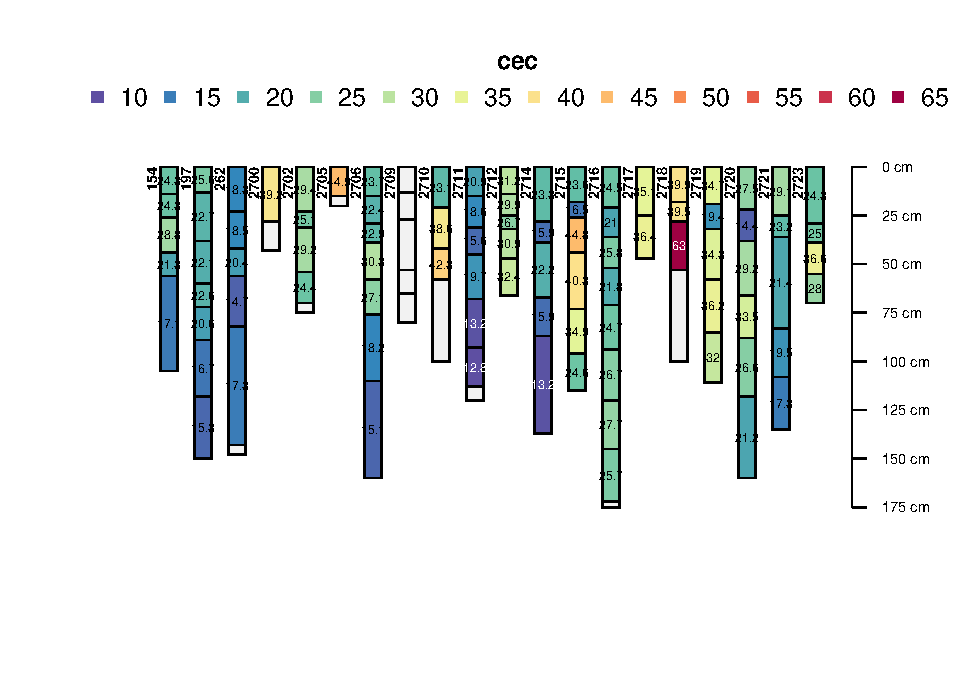
\includegraphics{GSNmap_Technical_Manual_files/figure-latex/unnamed-chunk-7-1.pdf}

\begin{Shaded}
\begin{Highlighting}[]
\DocumentationTok{\#\# 4.4 {-} check data integrity {-}{-}{-}{-}{-}{-}{-}{-}{-}{-}{-}{-}{-}{-}{-}{-}{-}{-}{-}{-}{-}{-}{-}{-}{-}{-}{-}{-}{-}{-}{-}{-}{-}{-}{-}{-}{-}{-}{-}{-}{-}{-}{-}{-}{-}{-}{-}{-}{-}{-}}
\CommentTok{\# A valid profile is TRUE if all of the following criteria are false:}
\CommentTok{\#    + depthLogic : boolean, errors related to depth logic}
\CommentTok{\#    + sameDepth : boolean, errors related to same top/bottom depths}
\CommentTok{\#    + missingDepth : boolean, NA in top / bottom depths}
\CommentTok{\#    + overlapOrGap : boolean, gaps or overlap in adjacent horizons}
\NormalTok{aqp}\SpecialCharTok{::}\FunctionTok{checkHzDepthLogic}\NormalTok{(profiles)}
\end{Highlighting}
\end{Shaded}

\begin{verbatim}
##     ProfID valid depthLogic sameDepth missingDepth overlapOrGap
## 1      154  TRUE      FALSE     FALSE        FALSE        FALSE
## 2      197  TRUE      FALSE     FALSE        FALSE        FALSE
## 3      262  TRUE      FALSE     FALSE        FALSE        FALSE
## 4     2700  TRUE      FALSE     FALSE        FALSE        FALSE
## 5     2702  TRUE      FALSE     FALSE        FALSE        FALSE
## 6     2705  TRUE      FALSE     FALSE        FALSE        FALSE
## 7     2706  TRUE      FALSE     FALSE        FALSE        FALSE
## 8     2709  TRUE      FALSE     FALSE        FALSE        FALSE
## 9     2710  TRUE      FALSE     FALSE        FALSE        FALSE
## 10    2711  TRUE      FALSE     FALSE        FALSE        FALSE
## 11    2712  TRUE      FALSE     FALSE        FALSE        FALSE
## 12    2714  TRUE      FALSE     FALSE        FALSE        FALSE
## 13    2715  TRUE      FALSE     FALSE        FALSE        FALSE
## 14    2716  TRUE      FALSE     FALSE        FALSE        FALSE
## 15    2717  TRUE      FALSE     FALSE        FALSE        FALSE
## 16    2718  TRUE      FALSE     FALSE        FALSE        FALSE
## 17    2719  TRUE      FALSE     FALSE        FALSE        FALSE
## 18    2720  TRUE      FALSE     FALSE        FALSE        FALSE
## 19    2721  TRUE      FALSE     FALSE        FALSE        FALSE
## 20    2723  TRUE      FALSE     FALSE        FALSE        FALSE
## 21    2725  TRUE      FALSE     FALSE        FALSE        FALSE
## 22    2726  TRUE      FALSE     FALSE        FALSE        FALSE
## 23    2761  TRUE      FALSE     FALSE        FALSE        FALSE
## 24    2762  TRUE      FALSE     FALSE        FALSE        FALSE
## 25    2763  TRUE      FALSE     FALSE        FALSE        FALSE
## 26    2764  TRUE      FALSE     FALSE        FALSE        FALSE
## 27    2767  TRUE      FALSE     FALSE        FALSE        FALSE
## 28    2768  TRUE      FALSE     FALSE        FALSE        FALSE
## 29    2769  TRUE      FALSE     FALSE        FALSE        FALSE
## 30    2770  TRUE      FALSE     FALSE        FALSE        FALSE
## 31    2771  TRUE      FALSE     FALSE        FALSE        FALSE
## 32    2772  TRUE      FALSE     FALSE        FALSE        FALSE
## 33    2773  TRUE      FALSE     FALSE        FALSE        FALSE
## 34    2774  TRUE      FALSE     FALSE        FALSE        FALSE
## 35    2775  TRUE      FALSE     FALSE        FALSE        FALSE
## 36    2796  TRUE      FALSE     FALSE        FALSE        FALSE
## 37    2797  TRUE      FALSE     FALSE        FALSE        FALSE
## 38    2798  TRUE      FALSE     FALSE        FALSE        FALSE
## 39    2799  TRUE      FALSE     FALSE        FALSE        FALSE
## 40    2800  TRUE      FALSE     FALSE        FALSE        FALSE
## 41    2801  TRUE      FALSE     FALSE        FALSE        FALSE
## 42    2802  TRUE      FALSE     FALSE        FALSE        FALSE
## 43    2803  TRUE      FALSE     FALSE        FALSE        FALSE
## 44    2804  TRUE      FALSE     FALSE        FALSE        FALSE
## 45    2805  TRUE      FALSE     FALSE        FALSE        FALSE
## 46    2806  TRUE      FALSE     FALSE        FALSE        FALSE
## 47    2807  TRUE      FALSE     FALSE        FALSE        FALSE
## 48    2808  TRUE      FALSE     FALSE        FALSE        FALSE
## 49    2809  TRUE      FALSE     FALSE        FALSE        FALSE
## 50    2810  TRUE      FALSE     FALSE        FALSE        FALSE
## 51    2811  TRUE      FALSE     FALSE        FALSE        FALSE
## 52    2812  TRUE      FALSE     FALSE        FALSE        FALSE
## 53    2813  TRUE      FALSE     FALSE        FALSE        FALSE
## 54    2814  TRUE      FALSE     FALSE        FALSE        FALSE
## 55    2815  TRUE      FALSE     FALSE        FALSE        FALSE
## 56    2816  TRUE      FALSE     FALSE        FALSE        FALSE
## 57    2817  TRUE      FALSE     FALSE        FALSE        FALSE
## 58    2818  TRUE      FALSE     FALSE        FALSE        FALSE
## 59    2819  TRUE      FALSE     FALSE        FALSE        FALSE
## 60    2820  TRUE      FALSE     FALSE        FALSE        FALSE
## 61    2821  TRUE      FALSE     FALSE        FALSE        FALSE
## 62    2822  TRUE      FALSE     FALSE        FALSE        FALSE
## 63    2823  TRUE      FALSE     FALSE        FALSE        FALSE
## 64    2824  TRUE      FALSE     FALSE        FALSE        FALSE
## 65    2825  TRUE      FALSE     FALSE        FALSE        FALSE
## 66    2826  TRUE      FALSE     FALSE        FALSE        FALSE
## 67    2827  TRUE      FALSE     FALSE        FALSE        FALSE
## 68    2828  TRUE      FALSE     FALSE        FALSE        FALSE
## 69    2891  TRUE      FALSE     FALSE        FALSE        FALSE
## 70    2892  TRUE      FALSE     FALSE        FALSE        FALSE
## 71    2911  TRUE      FALSE     FALSE        FALSE        FALSE
## 72    2948  TRUE      FALSE     FALSE        FALSE        FALSE
## 73    2979  TRUE      FALSE     FALSE        FALSE        FALSE
## 74    3026  TRUE      FALSE     FALSE        FALSE        FALSE
## 75    3027  TRUE      FALSE     FALSE        FALSE        FALSE
## 76    3029  TRUE      FALSE     FALSE        FALSE        FALSE
## 77    3172  TRUE      FALSE     FALSE        FALSE        FALSE
## 78    3174  TRUE      FALSE     FALSE        FALSE        FALSE
## 79    3175  TRUE      FALSE     FALSE        FALSE        FALSE
## 80    3204  TRUE      FALSE     FALSE        FALSE        FALSE
## 81      51  TRUE      FALSE     FALSE        FALSE        FALSE
## 82    6180  TRUE      FALSE     FALSE        FALSE        FALSE
## 83    6181  TRUE      FALSE     FALSE        FALSE        FALSE
## 84    6182  TRUE      FALSE     FALSE        FALSE        FALSE
## 85    6506  TRUE      FALSE     FALSE        FALSE        FALSE
## 86    6507  TRUE      FALSE     FALSE        FALSE        FALSE
## 87    6508  TRUE      FALSE     FALSE        FALSE        FALSE
## 88    6509  TRUE      FALSE     FALSE        FALSE        FALSE
## 89    6510  TRUE      FALSE     FALSE        FALSE        FALSE
## 90    6511  TRUE      FALSE     FALSE        FALSE        FALSE
## 91    6512  TRUE      FALSE     FALSE        FALSE        FALSE
## 92    6513  TRUE      FALSE     FALSE        FALSE        FALSE
## 93    6516  TRUE      FALSE     FALSE        FALSE        FALSE
## 94    6518  TRUE      FALSE     FALSE        FALSE        FALSE
## 95    6519  TRUE      FALSE     FALSE        FALSE        FALSE
## 96    6520  TRUE      FALSE     FALSE        FALSE        FALSE
## 97    6521  TRUE      FALSE     FALSE        FALSE        FALSE
## 98    6522  TRUE      FALSE     FALSE        FALSE        FALSE
## 99    6523  TRUE      FALSE     FALSE        FALSE        FALSE
## 100   6524  TRUE      FALSE     FALSE        FALSE        FALSE
## 101   6525  TRUE      FALSE     FALSE        FALSE        FALSE
## 102   6526  TRUE      FALSE     FALSE        FALSE        FALSE
## 103   6534  TRUE      FALSE     FALSE        FALSE        FALSE
## 104   6535  TRUE      FALSE     FALSE        FALSE        FALSE
## 105   6536  TRUE      FALSE     FALSE        FALSE        FALSE
## 106   6537  TRUE      FALSE     FALSE        FALSE        FALSE
## 107   6539  TRUE      FALSE     FALSE        FALSE        FALSE
## 108   6540  TRUE      FALSE     FALSE        FALSE        FALSE
## 109   6541  TRUE      FALSE     FALSE        FALSE        FALSE
## 110   6542  TRUE      FALSE     FALSE        FALSE        FALSE
## 111   6543  TRUE      FALSE     FALSE        FALSE        FALSE
## 112   6544  TRUE      FALSE     FALSE        FALSE        FALSE
## 113   6545  TRUE      FALSE     FALSE        FALSE        FALSE
## 114   6548  TRUE      FALSE     FALSE        FALSE        FALSE
## 115   6555  TRUE      FALSE     FALSE        FALSE        FALSE
## 116   6556  TRUE      FALSE     FALSE        FALSE        FALSE
## 117   6557  TRUE      FALSE     FALSE        FALSE        FALSE
## 118   6558  TRUE      FALSE     FALSE        FALSE        FALSE
## 119   6559  TRUE      FALSE     FALSE        FALSE        FALSE
## 120   6561  TRUE      FALSE     FALSE        FALSE        FALSE
## 121   6562  TRUE      FALSE     FALSE        FALSE        FALSE
## 122   6563  TRUE      FALSE     FALSE        FALSE        FALSE
## 123   6564  TRUE      FALSE     FALSE        FALSE        FALSE
## 124   6565  TRUE      FALSE     FALSE        FALSE        FALSE
## 125   6566 FALSE      FALSE     FALSE        FALSE         TRUE
## 126   6567  TRUE      FALSE     FALSE        FALSE        FALSE
## 127   6569  TRUE      FALSE     FALSE        FALSE        FALSE
## 128   6571  TRUE      FALSE     FALSE        FALSE        FALSE
## 129   6572  TRUE      FALSE     FALSE        FALSE        FALSE
## 130   6578  TRUE      FALSE     FALSE        FALSE        FALSE
## 131   6579  TRUE      FALSE     FALSE        FALSE        FALSE
## 132   6585  TRUE      FALSE     FALSE        FALSE        FALSE
## 133   6606  TRUE      FALSE     FALSE        FALSE        FALSE
## 134   6695  TRUE      FALSE     FALSE        FALSE        FALSE
## 135   6697  TRUE      FALSE     FALSE        FALSE        FALSE
## 136   6698  TRUE      FALSE     FALSE        FALSE        FALSE
## 137   6699  TRUE      FALSE     FALSE        FALSE        FALSE
## 138   6700  TRUE      FALSE     FALSE        FALSE        FALSE
## 139   6701  TRUE      FALSE     FALSE        FALSE        FALSE
## 140   6702  TRUE      FALSE     FALSE        FALSE        FALSE
## 141   6703  TRUE      FALSE     FALSE        FALSE        FALSE
## 142   6706  TRUE      FALSE     FALSE        FALSE        FALSE
## 143   6708  TRUE      FALSE     FALSE        FALSE        FALSE
## 144   6709  TRUE      FALSE     FALSE        FALSE        FALSE
## 145   6711  TRUE      FALSE     FALSE        FALSE        FALSE
## 146   6717  TRUE      FALSE     FALSE        FALSE        FALSE
## 147   6720  TRUE      FALSE     FALSE        FALSE        FALSE
## 148   6721  TRUE      FALSE     FALSE        FALSE        FALSE
## 149   6722  TRUE      FALSE     FALSE        FALSE        FALSE
## 150   6723  TRUE      FALSE     FALSE        FALSE        FALSE
## 151   6724  TRUE      FALSE     FALSE        FALSE        FALSE
## 152   6726  TRUE      FALSE     FALSE        FALSE        FALSE
## 153   6727  TRUE      FALSE     FALSE        FALSE        FALSE
## 154   6729  TRUE      FALSE     FALSE        FALSE        FALSE
## 155   6731  TRUE      FALSE     FALSE        FALSE        FALSE
## 156   6732  TRUE      FALSE     FALSE        FALSE        FALSE
## 157   6733  TRUE      FALSE     FALSE        FALSE        FALSE
## 158   6752  TRUE      FALSE     FALSE        FALSE        FALSE
## 159   6753  TRUE      FALSE     FALSE        FALSE        FALSE
## 160   6754  TRUE      FALSE     FALSE        FALSE        FALSE
## 161   6902  TRUE      FALSE     FALSE        FALSE        FALSE
## 162   6903  TRUE      FALSE     FALSE        FALSE        FALSE
## 163   6913  TRUE      FALSE     FALSE        FALSE        FALSE
## 164   6915  TRUE      FALSE     FALSE        FALSE        FALSE
## 165   6916  TRUE      FALSE     FALSE        FALSE        FALSE
## 166   6921  TRUE      FALSE     FALSE        FALSE        FALSE
## 167   6922  TRUE      FALSE     FALSE        FALSE        FALSE
## 168   6923  TRUE      FALSE     FALSE        FALSE        FALSE
## 169   6924  TRUE      FALSE     FALSE        FALSE        FALSE
## 170   6947  TRUE      FALSE     FALSE        FALSE        FALSE
## 171   6948  TRUE      FALSE     FALSE        FALSE        FALSE
## 172   6950  TRUE      FALSE     FALSE        FALSE        FALSE
## 173   6958  TRUE      FALSE     FALSE        FALSE        FALSE
## 174   6959  TRUE      FALSE     FALSE        FALSE        FALSE
## 175   6960  TRUE      FALSE     FALSE        FALSE        FALSE
## 176   6961  TRUE      FALSE     FALSE        FALSE        FALSE
## 177   6962  TRUE      FALSE     FALSE        FALSE        FALSE
## 178   7002  TRUE      FALSE     FALSE        FALSE        FALSE
## 179   7092  TRUE      FALSE     FALSE        FALSE        FALSE
## 180   7093  TRUE      FALSE     FALSE        FALSE        FALSE
## 181   7094  TRUE      FALSE     FALSE        FALSE        FALSE
## 182   7123  TRUE      FALSE     FALSE        FALSE        FALSE
## 183   7124  TRUE      FALSE     FALSE        FALSE        FALSE
## 184   7125  TRUE      FALSE     FALSE        FALSE        FALSE
## 185   7127  TRUE      FALSE     FALSE        FALSE        FALSE
## 186   7131  TRUE      FALSE     FALSE        FALSE        FALSE
## 187   7132  TRUE      FALSE     FALSE        FALSE        FALSE
## 188   7133  TRUE      FALSE     FALSE        FALSE        FALSE
## 189   7134  TRUE      FALSE     FALSE        FALSE        FALSE
## 190   7136  TRUE      FALSE     FALSE        FALSE        FALSE
## 191   7137  TRUE      FALSE     FALSE        FALSE        FALSE
## 192   7138  TRUE      FALSE     FALSE        FALSE        FALSE
## 193   7139  TRUE      FALSE     FALSE        FALSE        FALSE
## 194   7140  TRUE      FALSE     FALSE        FALSE        FALSE
## 195   7141  TRUE      FALSE     FALSE        FALSE        FALSE
## 196   7142  TRUE      FALSE     FALSE        FALSE        FALSE
## 197   7145  TRUE      FALSE     FALSE        FALSE        FALSE
## 198   7153  TRUE      FALSE     FALSE        FALSE        FALSE
## 199   7154  TRUE      FALSE     FALSE        FALSE        FALSE
## 200   7155  TRUE      FALSE     FALSE        FALSE        FALSE
## 201   7156  TRUE      FALSE     FALSE        FALSE        FALSE
## 202   7157  TRUE      FALSE     FALSE        FALSE        FALSE
## 203   7158  TRUE      FALSE     FALSE        FALSE        FALSE
## 204   7159  TRUE      FALSE     FALSE        FALSE        FALSE
## 205   7161  TRUE      FALSE     FALSE        FALSE        FALSE
## 206   7162  TRUE      FALSE     FALSE        FALSE        FALSE
## 207   7163  TRUE      FALSE     FALSE        FALSE        FALSE
## 208   7164  TRUE      FALSE     FALSE        FALSE        FALSE
## 209   7165  TRUE      FALSE     FALSE        FALSE        FALSE
## 210   7166  TRUE      FALSE     FALSE        FALSE        FALSE
## 211   7170  TRUE      FALSE     FALSE        FALSE        FALSE
## 212   7172  TRUE      FALSE     FALSE        FALSE        FALSE
## 213   7174  TRUE      FALSE     FALSE        FALSE        FALSE
## 214   7175  TRUE      FALSE     FALSE        FALSE        FALSE
## 215   7176  TRUE      FALSE     FALSE        FALSE        FALSE
## 216   7202  TRUE      FALSE     FALSE        FALSE        FALSE
## 217   7207  TRUE      FALSE     FALSE        FALSE        FALSE
## 218   7208  TRUE      FALSE     FALSE        FALSE        FALSE
## 219   7209  TRUE      FALSE     FALSE        FALSE        FALSE
## 220   7210  TRUE      FALSE     FALSE        FALSE        FALSE
## 221   7211  TRUE      FALSE     FALSE        FALSE        FALSE
## 222   7212  TRUE      FALSE     FALSE        FALSE        FALSE
## 223   7213  TRUE      FALSE     FALSE        FALSE        FALSE
## 224   7219  TRUE      FALSE     FALSE        FALSE        FALSE
## 225   7220  TRUE      FALSE     FALSE        FALSE        FALSE
## 226   7222  TRUE      FALSE     FALSE        FALSE        FALSE
## 227   7223  TRUE      FALSE     FALSE        FALSE        FALSE
## 228   7224  TRUE      FALSE     FALSE        FALSE        FALSE
## 229   7225  TRUE      FALSE     FALSE        FALSE        FALSE
## 230   7226  TRUE      FALSE     FALSE        FALSE        FALSE
## 231   7228  TRUE      FALSE     FALSE        FALSE        FALSE
## 232   7329  TRUE      FALSE     FALSE        FALSE        FALSE
## 233   7330  TRUE      FALSE     FALSE        FALSE        FALSE
## 234   7331  TRUE      FALSE     FALSE        FALSE        FALSE
## 235   7336  TRUE      FALSE     FALSE        FALSE        FALSE
## 236   7337  TRUE      FALSE     FALSE        FALSE        FALSE
## 237   7338  TRUE      FALSE     FALSE        FALSE        FALSE
## 238   7339  TRUE      FALSE     FALSE        FALSE        FALSE
## 239   7340  TRUE      FALSE     FALSE        FALSE        FALSE
## 240   7341  TRUE      FALSE     FALSE        FALSE        FALSE
## 241   7342  TRUE      FALSE     FALSE        FALSE        FALSE
## 242   7343  TRUE      FALSE     FALSE        FALSE        FALSE
## 243   7344  TRUE      FALSE     FALSE        FALSE        FALSE
## 244   7345  TRUE      FALSE     FALSE        FALSE        FALSE
## 245   7346  TRUE      FALSE     FALSE        FALSE        FALSE
## 246   7349  TRUE      FALSE     FALSE        FALSE        FALSE
## 247   7350  TRUE      FALSE     FALSE        FALSE        FALSE
## 248   7351  TRUE      FALSE     FALSE        FALSE        FALSE
## 249   7352  TRUE      FALSE     FALSE        FALSE        FALSE
## 250   7353  TRUE      FALSE     FALSE        FALSE        FALSE
## 251   7354  TRUE      FALSE     FALSE        FALSE        FALSE
## 252   7355  TRUE      FALSE     FALSE        FALSE        FALSE
## 253   7356  TRUE      FALSE     FALSE        FALSE        FALSE
## 254   7359  TRUE      FALSE     FALSE        FALSE        FALSE
## 255   7360  TRUE      FALSE     FALSE        FALSE        FALSE
## 256   7361  TRUE      FALSE     FALSE        FALSE        FALSE
## 257   7362  TRUE      FALSE     FALSE        FALSE        FALSE
## 258   7363  TRUE      FALSE     FALSE        FALSE        FALSE
## 259   7364  TRUE      FALSE     FALSE        FALSE        FALSE
## 260   7365  TRUE      FALSE     FALSE        FALSE        FALSE
## 261   7367  TRUE      FALSE     FALSE        FALSE        FALSE
## 262   7368  TRUE      FALSE     FALSE        FALSE        FALSE
## 263   7374  TRUE      FALSE     FALSE        FALSE        FALSE
## 264   7376  TRUE      FALSE     FALSE        FALSE        FALSE
## 265   7378  TRUE      FALSE     FALSE        FALSE        FALSE
## 266   7379  TRUE      FALSE     FALSE        FALSE        FALSE
## 267   7382  TRUE      FALSE     FALSE        FALSE        FALSE
## 268   7383  TRUE      FALSE     FALSE        FALSE        FALSE
## 269   7384  TRUE      FALSE     FALSE        FALSE        FALSE
## 270   7385  TRUE      FALSE     FALSE        FALSE        FALSE
## 271   7386  TRUE      FALSE     FALSE        FALSE        FALSE
## 272   7387  TRUE      FALSE     FALSE        FALSE        FALSE
## 273   7388  TRUE      FALSE     FALSE        FALSE        FALSE
## 274   7389  TRUE      FALSE     FALSE        FALSE        FALSE
## 275   7390  TRUE      FALSE     FALSE        FALSE        FALSE
## 276   7391  TRUE      FALSE     FALSE        FALSE        FALSE
## 277   7392  TRUE      FALSE     FALSE        FALSE        FALSE
## 278   7393  TRUE      FALSE     FALSE        FALSE        FALSE
## 279   7394  TRUE      FALSE     FALSE        FALSE        FALSE
## 280   7395  TRUE      FALSE     FALSE        FALSE        FALSE
## 281   7408  TRUE      FALSE     FALSE        FALSE        FALSE
## 282   7410 FALSE      FALSE     FALSE        FALSE         TRUE
## 283   7411  TRUE      FALSE     FALSE        FALSE        FALSE
## 284   7420  TRUE      FALSE     FALSE        FALSE        FALSE
## 285   7421  TRUE      FALSE     FALSE        FALSE        FALSE
## 286   7422  TRUE      FALSE     FALSE        FALSE        FALSE
## 287   7423  TRUE      FALSE     FALSE        FALSE        FALSE
## 288   7424  TRUE      FALSE     FALSE        FALSE        FALSE
## 289   7426  TRUE      FALSE     FALSE        FALSE        FALSE
## 290   7434  TRUE      FALSE     FALSE        FALSE        FALSE
## 291   7435  TRUE      FALSE     FALSE        FALSE        FALSE
## 292   7436  TRUE      FALSE     FALSE        FALSE        FALSE
## 293   7437  TRUE      FALSE     FALSE        FALSE        FALSE
## 294   7438  TRUE      FALSE     FALSE        FALSE        FALSE
## 295   7439  TRUE      FALSE     FALSE        FALSE        FALSE
## 296   7440  TRUE      FALSE     FALSE        FALSE        FALSE
## 297   7441  TRUE      FALSE     FALSE        FALSE        FALSE
## 298   7442  TRUE      FALSE     FALSE        FALSE        FALSE
## 299   7443  TRUE      FALSE     FALSE        FALSE        FALSE
## 300   7444  TRUE      FALSE     FALSE        FALSE        FALSE
## 301   7447  TRUE      FALSE     FALSE        FALSE        FALSE
## 302   7448  TRUE      FALSE     FALSE        FALSE        FALSE
## 303   7451  TRUE      FALSE     FALSE        FALSE        FALSE
## 304   7452  TRUE      FALSE     FALSE        FALSE        FALSE
## 305   7455  TRUE      FALSE     FALSE        FALSE        FALSE
## 306   7456  TRUE      FALSE     FALSE        FALSE        FALSE
## 307   7457  TRUE      FALSE     FALSE        FALSE        FALSE
## 308   7458  TRUE      FALSE     FALSE        FALSE        FALSE
## 309   7459  TRUE      FALSE     FALSE        FALSE        FALSE
## 310   7687  TRUE      FALSE     FALSE        FALSE        FALSE
## 311   7697  TRUE      FALSE     FALSE        FALSE        FALSE
## 312   7726  TRUE      FALSE     FALSE        FALSE        FALSE
## 313   7833  TRUE      FALSE     FALSE        FALSE        FALSE
## 314   7882  TRUE      FALSE     FALSE        FALSE        FALSE
## 315   7907  TRUE      FALSE     FALSE        FALSE        FALSE
## 316   7922  TRUE      FALSE     FALSE        FALSE        FALSE
## 317   7933  TRUE      FALSE     FALSE        FALSE        FALSE
## 318   7937  TRUE      FALSE     FALSE        FALSE        FALSE
## 319   7941  TRUE      FALSE     FALSE        FALSE        FALSE
## 320   7950  TRUE      FALSE     FALSE        FALSE        FALSE
## 321   7955  TRUE      FALSE     FALSE        FALSE        FALSE
## 322   7965  TRUE      FALSE     FALSE        FALSE        FALSE
## 323   7966  TRUE      FALSE     FALSE        FALSE        FALSE
## 324   7973  TRUE      FALSE     FALSE        FALSE        FALSE
## 325   7978  TRUE      FALSE     FALSE        FALSE        FALSE
## 326   7981  TRUE      FALSE     FALSE        FALSE        FALSE
## 327   7986  TRUE      FALSE     FALSE        FALSE        FALSE
## 328   7987  TRUE      FALSE     FALSE        FALSE        FALSE
## 329   7988  TRUE      FALSE     FALSE        FALSE        FALSE
## 330   7990  TRUE      FALSE     FALSE        FALSE        FALSE
## 331   7991  TRUE      FALSE     FALSE        FALSE        FALSE
## 332   7993  TRUE      FALSE     FALSE        FALSE        FALSE
## 333   7994  TRUE      FALSE     FALSE        FALSE        FALSE
## 334   7997  TRUE      FALSE     FALSE        FALSE        FALSE
## 335   8000  TRUE      FALSE     FALSE        FALSE        FALSE
## 336   8002 FALSE      FALSE     FALSE        FALSE         TRUE
## 337   8004  TRUE      FALSE     FALSE        FALSE        FALSE
## 338   8006  TRUE      FALSE     FALSE        FALSE        FALSE
## 339   8010  TRUE      FALSE     FALSE        FALSE        FALSE
## 340   8011  TRUE      FALSE     FALSE        FALSE        FALSE
## 341   8012  TRUE      FALSE     FALSE        FALSE        FALSE
## 342   8018  TRUE      FALSE     FALSE        FALSE        FALSE
## 343   8021  TRUE      FALSE     FALSE        FALSE        FALSE
## 344   8023  TRUE      FALSE     FALSE        FALSE        FALSE
## 345   8025  TRUE      FALSE     FALSE        FALSE        FALSE
## 346   8026  TRUE      FALSE     FALSE        FALSE        FALSE
## 347   8027  TRUE      FALSE     FALSE        FALSE        FALSE
## 348   8028  TRUE      FALSE     FALSE        FALSE        FALSE
## 349   8067  TRUE      FALSE     FALSE        FALSE        FALSE
## 350   8069  TRUE      FALSE     FALSE        FALSE        FALSE
## 351   8070  TRUE      FALSE     FALSE        FALSE        FALSE
## 352   8075  TRUE      FALSE     FALSE        FALSE        FALSE
## 353   8083  TRUE      FALSE     FALSE        FALSE        FALSE
## 354   8093  TRUE      FALSE     FALSE        FALSE        FALSE
## 355   8099  TRUE      FALSE     FALSE        FALSE        FALSE
## 356   8122  TRUE      FALSE     FALSE        FALSE        FALSE
## 357   8128  TRUE      FALSE     FALSE        FALSE        FALSE
\end{verbatim}

\begin{Shaded}
\begin{Highlighting}[]
\CommentTok{\# Identify non{-}valid profiles }
\NormalTok{dl }\OtherTok{\textless{}{-}} \FunctionTok{checkHzDepthLogic}\NormalTok{(profiles)}
\NormalTok{dl[dl}\SpecialCharTok{$}\NormalTok{depthLogic}\SpecialCharTok{==}\NormalTok{T }\SpecialCharTok{|}\NormalTok{ dl}\SpecialCharTok{$}\NormalTok{sameDepth}\SpecialCharTok{==}\NormalTok{T }\SpecialCharTok{|}\NormalTok{ dl}\SpecialCharTok{$}\NormalTok{missingDepth}\SpecialCharTok{==}\NormalTok{T }\SpecialCharTok{|}\NormalTok{ dl}\SpecialCharTok{$}\NormalTok{overlapOrGap}\SpecialCharTok{==}\NormalTok{T,}\StringTok{"ProfID"}\NormalTok{]}
\end{Highlighting}
\end{Shaded}

\begin{verbatim}
## [1] 6566 7410 8002
\end{verbatim}

If there are profiles that violate the depth logic rules (i.e.~overlapping horizons), they can be selected and checked through the Profile ID. In the following step, only profiles with valid horizon logic are selected. Finally, the soil profile collection is re-converted to a dataframe. With this, the quality check is finished.

\begin{Shaded}
\begin{Highlighting}[]
\CommentTok{\# visualize some of these profiles by the pid}
\FunctionTok{subset}\NormalTok{(profiles, }\FunctionTok{grepl}\NormalTok{(}\DecValTok{6566}\NormalTok{, ProfID, }\AttributeTok{ignore.case =} \ConstantTok{TRUE}\NormalTok{))}
\end{Highlighting}
\end{Shaded}

\begin{verbatim}
## SoilProfileCollection with 1 profiles and 4 horizons
## profile ID: ProfID  |  horizon ID: hzID 
## Depth range: 80 - 80 cm
## 
## ----- Horizons (4 / 4 rows  |  10 / 10 columns) -----
##  ProfID hzID top bottom HorID  ph   k  soc bd  cec
##    6566  643   0     16 29463 9.4 1.5 2.02 NA 14.0
##    6566  644  16     25 29464 9.5 1.2 0.91 NA 13.0
##    6566  645  26     55 29465 9.1 2.6 0.42 NA 22.7
##    6566  646  55     80 29466 9.0 2.2 0.19 NA 18.8
## 
## ----- Sites (1 / 1 rows  |  3 / 3 columns) -----
##  ProfID         x         y
##    6566 -58.20125 -37.92759
## 
## Spatial Data:
## [EMPTY]
\end{verbatim}

\begin{Shaded}
\begin{Highlighting}[]
\FunctionTok{subset}\NormalTok{(profiles, }\FunctionTok{grepl}\NormalTok{(}\DecValTok{6915}\NormalTok{, ProfID, }\AttributeTok{ignore.case =} \ConstantTok{TRUE}\NormalTok{))}
\end{Highlighting}
\end{Shaded}

\begin{verbatim}
## SoilProfileCollection with 1 profiles and 7 horizons
## profile ID: ProfID  |  horizon ID: hzID 
## Depth range: 140 - 140 cm
## 
## ----- Horizons (6 / 7 rows  |  10 / 10 columns) -----
##  ProfID hzID top bottom HorID  ph   k   soc bd  cec
##    6915  864   0      6 31278 6.0 2.8 15.78 NA 46.6
##    6915  865   6     14 31279 6.7 1.8  5.65 NA 31.8
##    6915  866  14     21 31280 7.5 0.9  2.02 NA 17.3
##    6915  867  21     35 31281 7.6 1.0  0.45 NA  9.1
##    6915  868  35     65 31282 8.2 2.3  0.41 NA 29.7
##    6915  869  65     87 31283 8.5 2.7  0.23 NA 33.1
## [... more horizons ...]
## 
## ----- Sites (1 / 1 rows  |  3 / 3 columns) -----
##  ProfID         x         y
##    6915 -58.23173 -37.59698
## 
## Spatial Data:
## [EMPTY]
\end{verbatim}

\begin{Shaded}
\begin{Highlighting}[]
\FunctionTok{subset}\NormalTok{(profiles, }\FunctionTok{grepl}\NormalTok{(}\DecValTok{7726}\NormalTok{, ProfID, }\AttributeTok{ignore.case =} \ConstantTok{TRUE}\NormalTok{))}
\end{Highlighting}
\end{Shaded}

\begin{verbatim}
## SoilProfileCollection with 1 profiles and 5 horizons
## profile ID: ProfID  |  horizon ID: hzID 
## Depth range: 155 - 155 cm
## 
## ----- Horizons (5 / 5 rows  |  10 / 10 columns) -----
##  ProfID hzID top bottom HorID  ph   k   soc bd  cec
##    7726 1581   0     27 35695 6.5 1.2 19.00 NA 27.0
##    7726 1582  27     38 35696 6.6 1.4  1.97 NA 24.8
##    7726 1583  38     70 35697 6.9 1.4  0.83 NA 29.7
##    7726 1584  70     97 35698 7.2 1.4  0.20 NA 18.0
##    7726 1585  97    155 35699 7.3 1.2    NA NA 13.8
## 
## ----- Sites (1 / 1 rows  |  3 / 3 columns) -----
##  ProfID        x         y
##    7726 -58.8281 -37.32196
## 
## Spatial Data:
## [EMPTY]
\end{verbatim}

\begin{Shaded}
\begin{Highlighting}[]
\DocumentationTok{\#\# 4.5 {-} keep only valid profiles {-}{-}{-}{-}{-}{-}{-}{-}{-}{-}{-}{-}{-}{-}{-}{-}{-}{-}{-}{-}{-}{-}{-}{-}{-}{-}{-}{-}{-}{-}{-}{-}{-}{-}{-}{-}{-}{-}{-}{-}{-}{-}{-}{-}{-}{-}}
\NormalTok{clean\_prof }\OtherTok{\textless{}{-}} \FunctionTok{HzDepthLogicSubset}\NormalTok{(profiles)}
\end{Highlighting}
\end{Shaded}

\begin{verbatim}
## dropping profiles with invalid depth logic, see `metadata(x)$removed.profiles`
\end{verbatim}

\begin{Shaded}
\begin{Highlighting}[]
\FunctionTok{metadata}\NormalTok{(clean\_prof)}\SpecialCharTok{$}\NormalTok{removed.profiles}
\end{Highlighting}
\end{Shaded}

\begin{verbatim}
## [1] 6566 7410 8002
\end{verbatim}

\begin{Shaded}
\begin{Highlighting}[]
\CommentTok{\# write\_rds(clean\_prof, "01{-}Data/soilProfileCollection.rds")}

\DocumentationTok{\#\# 4.6 convert soilProfileCollection to a table {-}{-}{-}{-}{-}{-}{-}{-}{-}{-}{-}{-}{-}{-}{-}{-}{-}{-}{-}{-}{-}{-}{-}{-}{-}{-}{-}{-}{-}{-}{-}{-}}
\NormalTok{dat }\OtherTok{\textless{}{-}} \FunctionTok{left\_join}\NormalTok{(clean\_prof}\SpecialCharTok{@}\NormalTok{site, clean\_prof}\SpecialCharTok{@}\NormalTok{horizons)}
\end{Highlighting}
\end{Shaded}

\begin{verbatim}
## Joining with `by = join_by(ProfID)`
\end{verbatim}

\begin{Shaded}
\begin{Highlighting}[]
\NormalTok{dat }\OtherTok{\textless{}{-}} \FunctionTok{select}\NormalTok{(dat, ProfID, HorID, x, y, top, bottom, ph}\SpecialCharTok{:}\NormalTok{cec )}
\end{Highlighting}
\end{Shaded}

\hypertarget{calculation-of-pedo-transfer-functions}{%
\section{Calculation of pedo-transfer functions}\label{calculation-of-pedo-transfer-functions}}

In the cases of single-layer samples, which is common in sampling for nutrient determination, a locally calibrated pedotransfer function (PTF) should be applied. PTF will be also required to harmonise the laboratory methods. Experts from the Global Soil Laboratory Network (GLOSOLAN) will provide advice in this regard.

Therefore, a customised function is introduced to our working environment. Users can write their own functions in \textbf{R}. This is often necessary when existing functions need to be customised or very specific calculations need to be performed. Functions greatly increase the efficiency of our code. For further information, it is recommendable to consult online resources on the topic (e.g.~\url{https://hbctraining.github.io/Intro-to-R/lessons/03_introR-functions-and-arguments.html}).

The function \texttt{estimateBD} below calculates various PTFs that estimate bulk density (BD). Which equation is used is determined by the user that has to choose one of the methods and also specify the SOC value of the respective horizon. The SOC values is first converted to OM by using the conversion factor of 1.724 and then inserted in the respective PTF. The return() command tells \textbf{R} which value to output.

\begin{Shaded}
\begin{Highlighting}[]
\CommentTok{\# 5 {-} Estimate BD using pedotransfer functions =================================}

\CommentTok{\# create the function with all PTF}
\NormalTok{method\_names }\OtherTok{\textless{}{-}} \FunctionTok{c}\NormalTok{(}\StringTok{"Saini1996"}\NormalTok{, }\StringTok{"Drew1973"}\NormalTok{, }\StringTok{"Jeffrey1979"}\NormalTok{, }\StringTok{"Grigal1989"}\NormalTok{, }
                  \StringTok{"Adams1973"}\NormalTok{, }\StringTok{"Honeyset\_Ratkowsky1989"}\NormalTok{) }

\NormalTok{estimateBD }\OtherTok{\textless{}{-}} \ControlFlowTok{function}\NormalTok{(}\AttributeTok{SOC=}\ConstantTok{NULL}\NormalTok{, }\AttributeTok{method=}\ConstantTok{NULL}\NormalTok{) \{}
\NormalTok{  OM }\OtherTok{\textless{}{-}}\NormalTok{ SOC }\SpecialCharTok{*} \FloatTok{1.724}
\NormalTok{  BD }\OtherTok{\textless{}{-}} \ControlFlowTok{switch}\NormalTok{(method,}
               \StringTok{"Saini1996"} \OtherTok{=} \FloatTok{1.62} \SpecialCharTok{{-}} \FloatTok{0.06} \SpecialCharTok{*}\NormalTok{ OM,}
               \StringTok{"Drew1973"} \OtherTok{=} \DecValTok{1} \SpecialCharTok{/}\NormalTok{ (}\FloatTok{0.6268} \SpecialCharTok{+} \FloatTok{0.0361} \SpecialCharTok{*}\NormalTok{ OM),}
               \StringTok{"Jeffrey1979"} \OtherTok{=} \FloatTok{1.482} \SpecialCharTok{{-}} \FloatTok{0.6786} \SpecialCharTok{*}\NormalTok{ (}\FunctionTok{log}\NormalTok{(OM)),}
               \StringTok{"Grigal1989"} \OtherTok{=} \FloatTok{0.669} \SpecialCharTok{+} \FloatTok{0.941} \SpecialCharTok{*} \FunctionTok{exp}\NormalTok{(}\DecValTok{1}\NormalTok{)}\SpecialCharTok{\^{}}\NormalTok{(}\SpecialCharTok{{-}}\FloatTok{0.06} \SpecialCharTok{*}\NormalTok{ OM),}
               \StringTok{"Adams1973"} \OtherTok{=} \DecValTok{100} \SpecialCharTok{/}\NormalTok{ (OM }\SpecialCharTok{/} \FloatTok{0.244} \SpecialCharTok{+}\NormalTok{ (}\DecValTok{100} \SpecialCharTok{{-}}\NormalTok{ OM) }\SpecialCharTok{/} \FloatTok{2.65}\NormalTok{),}
               \StringTok{"Honeyset\_Ratkowsky1989"} \OtherTok{=} \DecValTok{1} \SpecialCharTok{/}\NormalTok{ (}\FloatTok{0.564} \SpecialCharTok{+} \FloatTok{0.0556} \SpecialCharTok{*}\NormalTok{ OM),}
               \FunctionTok{stop}\NormalTok{(}\StringTok{"Invalid method specified."}\NormalTok{)}
\NormalTok{  )}
  \FunctionTok{return}\NormalTok{(BD)}
\NormalTok{\}}
\end{Highlighting}
\end{Shaded}

To apply the \texttt{estimateBD} function, first a test dataframe is created that includes the SOC values from the cleaned profile table as well as the respective existing BD measurements. The rows without values in one of the columns are excluded using the na.omit() function since we want to first evaluate the difference between estimated BDs and measured BDs.
Now, the test dataframe is complemented by the estimated BDs derived from the PTFs for each method. To add new columns to an existing dataframe one has to write on the left-hand side of the arrow the name of the existing dataframe object (in this case BD\_test), the dollar sign (\$), and the name of the new column. Here, the names are given according to the used BD PTF.

\begin{Shaded}
\begin{Highlighting}[]
\DocumentationTok{\#\# 5.1 {-} Select a pedotransfer function {-}{-}{-}{-}{-}{-}{-}{-}{-}{-}{-}{-}{-}{-}{-}{-}{-}{-}{-}{-}{-}{-}{-}{-}{-}{-}{-}{-}{-}{-}{-}{-}{-}{-}{-}{-}{-}{-}{-}{-}}
\CommentTok{\# Create a test dataset with BD and SOC data}
\NormalTok{BD\_test }\OtherTok{\textless{}{-}} \FunctionTok{data.frame}\NormalTok{(}\AttributeTok{SOC =}\NormalTok{ dat}\SpecialCharTok{$}\NormalTok{soc, }\AttributeTok{BD\_observed =}\NormalTok{ dat}\SpecialCharTok{$}\NormalTok{bd)}

\CommentTok{\# Remove missing values}
\NormalTok{BD\_test }\OtherTok{\textless{}{-}}\NormalTok{ BD\_test[}\FunctionTok{complete.cases}\NormalTok{(BD\_test),]}
\NormalTok{BD\_test }\OtherTok{\textless{}{-}} \FunctionTok{na.omit}\NormalTok{(BD\_test) }


\CommentTok{\# 5.2 {-} Estimate BLD for a subset using the pedotransfer functions {-}{-}{-}{-}{-}{-}{-}{-}{-}{-}{-}{-}}
\ControlFlowTok{for}\NormalTok{ (i }\ControlFlowTok{in}\NormalTok{ method\_names) \{}
\NormalTok{  BD\_test[[i]] }\OtherTok{\textless{}{-}} \FunctionTok{estimateBD}\NormalTok{(BD\_test}\SpecialCharTok{$}\NormalTok{SOC, }\AttributeTok{method =}\NormalTok{ i)}
\NormalTok{\}}

\CommentTok{\# Print the resulting data frame}
\NormalTok{BD\_test}
\end{Highlighting}
\end{Shaded}

\begin{verbatim}
##      SOC BD_observed Saini1996 Drew1973 Jeffrey1979 Grigal1989 Adams1973
## 367 1.64        1.16  1.450358 1.371991   0.7767016   1.463173  2.072261
## 373 2.38        1.26  1.373813 1.290451   0.5239880   1.404651  1.886665
## 374 0.50        1.49  1.568280 1.519946   1.5827721   1.562569  2.442399
## 376 2.05        1.14  1.407948 1.325584   0.6252763   1.430196  1.965153
## 377 0.44        1.36  1.574486 1.528622   1.6695198   1.568132  2.465577
## 386 0.75        1.43  1.542420 1.484831   1.3076235   1.539757  2.350336
## 387 0.75        1.38  1.542420 1.484831   1.3076235   1.539757  2.350336
## 389 3.20        0.87  1.288992 1.210718   0.3230883   1.344826  1.716329
## 394 1.11        1.25  1.505182 1.437024   1.0415837   1.507928  2.229331
##     Honeyset_Ratkowsky1989
## 367               1.386576
## 373               1.262414
## 374               1.634181
## 376               1.314922
## 377               1.649686
## 386               1.572597
## 387               1.572597
## 389               1.148456
## 394               1.491650
\end{verbatim}

The calculated BDs can now be compared using the \texttt{summary()} function. However, a faster and more accessible approach is to plot the different bulk densities for comparison. In case you are not familiar with the \texttt{plot()} function and its respective commands, it is recommendable to check one of the many online learning resources such as \url{https://intro2r.com/simple-base-r-plots.html}. The plot shows us both measured and estimated BD values as differently coloured lines.

\begin{Shaded}
\begin{Highlighting}[]
\DocumentationTok{\#\# 5.3 Compare results {-}{-}{-}{-}{-}{-}{-}{-}{-}{-}{-}{-}{-}{-}{-}{-}{-}{-}{-}{-}{-}{-}{-}{-}{-}{-}{-}{-}{-}{-}{-}{-}{-}{-}{-}{-}{-}{-}{-}{-}{-}{-}{-}{-}{-}{-}{-}{-}{-}{-}{-}{-}{-}{-}{-}{-}{-}}

\CommentTok{\# Observed values:}
\FunctionTok{summary}\NormalTok{(BD\_test)}
\end{Highlighting}
\end{Shaded}

\begin{verbatim}
##       SOC         BD_observed     Saini1996        Drew1973    
##  Min.   :0.440   Min.   :0.87   Min.   :1.289   Min.   :1.211  
##  1st Qu.:0.750   1st Qu.:1.16   1st Qu.:1.408   1st Qu.:1.326  
##  Median :1.110   Median :1.26   Median :1.505   Median :1.437  
##  Mean   :1.424   Mean   :1.26   Mean   :1.473   Mean   :1.406  
##  3rd Qu.:2.050   3rd Qu.:1.38   3rd Qu.:1.542   3rd Qu.:1.485  
##  Max.   :3.200   Max.   :1.49   Max.   :1.574   Max.   :1.529  
##   Jeffrey1979       Grigal1989      Adams1973     Honeyset_Ratkowsky1989
##  Min.   :0.3231   Min.   :1.345   Min.   :1.716   Min.   :1.148         
##  1st Qu.:0.6253   1st Qu.:1.430   1st Qu.:1.965   1st Qu.:1.315         
##  Median :1.0416   Median :1.508   Median :2.229   Median :1.492         
##  Mean   :1.0176   Mean   :1.485   Mean   :2.164   Mean   :1.448         
##  3rd Qu.:1.3076   3rd Qu.:1.540   3rd Qu.:2.350   3rd Qu.:1.573         
##  Max.   :1.6695   Max.   :1.568   Max.   :2.466   Max.   :1.650
\end{verbatim}

\begin{Shaded}
\begin{Highlighting}[]
\CommentTok{\# Compare data distributions for observed and predicted BLD}
\NormalTok{plot.bd }\OtherTok{\textless{}{-}}\NormalTok{ BD\_test }\SpecialCharTok{\%\textgreater{}\%}
  \FunctionTok{select}\NormalTok{(}\SpecialCharTok{{-}}\NormalTok{SOC) }\SpecialCharTok{\%\textgreater{}\%} 
  \FunctionTok{pivot\_longer}\NormalTok{(}\AttributeTok{cols =} \FunctionTok{c}\NormalTok{(}\StringTok{"BD\_observed"}\NormalTok{, }\StringTok{"Saini1996"}\NormalTok{, }\StringTok{"Drew1973"}\NormalTok{, }\StringTok{"Jeffrey1979"}\NormalTok{,}
                        \StringTok{"Grigal1989"}\NormalTok{, }\StringTok{"Adams1973"}\NormalTok{, }\StringTok{"Honeyset\_Ratkowsky1989"}\NormalTok{), }
               \AttributeTok{names\_to =} \StringTok{"Method"}\NormalTok{, }\AttributeTok{values\_to =} \StringTok{"BD"}\NormalTok{) }\SpecialCharTok{\%\textgreater{}\%} 
  \FunctionTok{ggplot}\NormalTok{(}\FunctionTok{aes}\NormalTok{(}\AttributeTok{x =}\NormalTok{ BD, }\AttributeTok{color =}\NormalTok{ Method)) }\SpecialCharTok{+} 
  \FunctionTok{geom\_density}\NormalTok{()}

\NormalTok{plot.bd}
\end{Highlighting}
\end{Shaded}

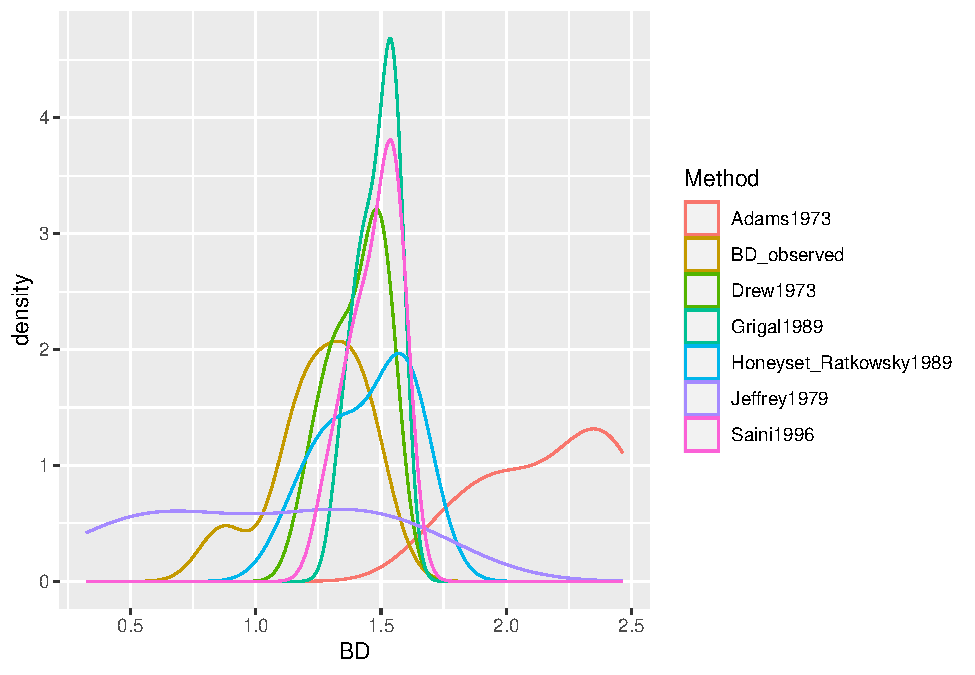
\includegraphics{GSNmap_Technical_Manual_files/figure-latex/unnamed-chunk-11-1.pdf}

\begin{Shaded}
\begin{Highlighting}[]
\CommentTok{\# Dymanic plot with plotly }
\NormalTok{plotly}\SpecialCharTok{::}\FunctionTok{ggplotly}\NormalTok{(plot.bd)}
\end{Highlighting}
\end{Shaded}

\begin{Shaded}
\begin{Highlighting}[]
\NormalTok{plotly}\SpecialCharTok{::}\FunctionTok{ggplotly}\NormalTok{(plot.bd) }
\end{Highlighting}
\end{Shaded}

\begin{Shaded}
\begin{Highlighting}[]
\CommentTok{\# Plot the Selected function again}
\NormalTok{BD\_test }\SpecialCharTok{\%\textgreater{}\%} 
  \FunctionTok{select}\NormalTok{(}\SpecialCharTok{{-}}\NormalTok{SOC) }\SpecialCharTok{\%\textgreater{}\%} 
  \FunctionTok{pivot\_longer}\NormalTok{(}\AttributeTok{cols =} \FunctionTok{c}\NormalTok{(}\StringTok{"BD\_observed"}\NormalTok{, }\StringTok{"Honeyset\_Ratkowsky1989"}\NormalTok{), }
               \AttributeTok{names\_to =} \StringTok{"Method"}\NormalTok{, }\AttributeTok{values\_to =} \StringTok{"BD"}\NormalTok{) }\SpecialCharTok{\%\textgreater{}\%} 
  \FunctionTok{ggplot}\NormalTok{(}\FunctionTok{aes}\NormalTok{(}\AttributeTok{x =}\NormalTok{ BD, }\AttributeTok{color =}\NormalTok{ Method)) }\SpecialCharTok{+} 
  \FunctionTok{geom\_density}\NormalTok{() }\SpecialCharTok{+} \FunctionTok{xlim}\NormalTok{(}\FunctionTok{c}\NormalTok{(}\DecValTok{0}\NormalTok{,}\FloatTok{2.5}\NormalTok{))}
\end{Highlighting}
\end{Shaded}

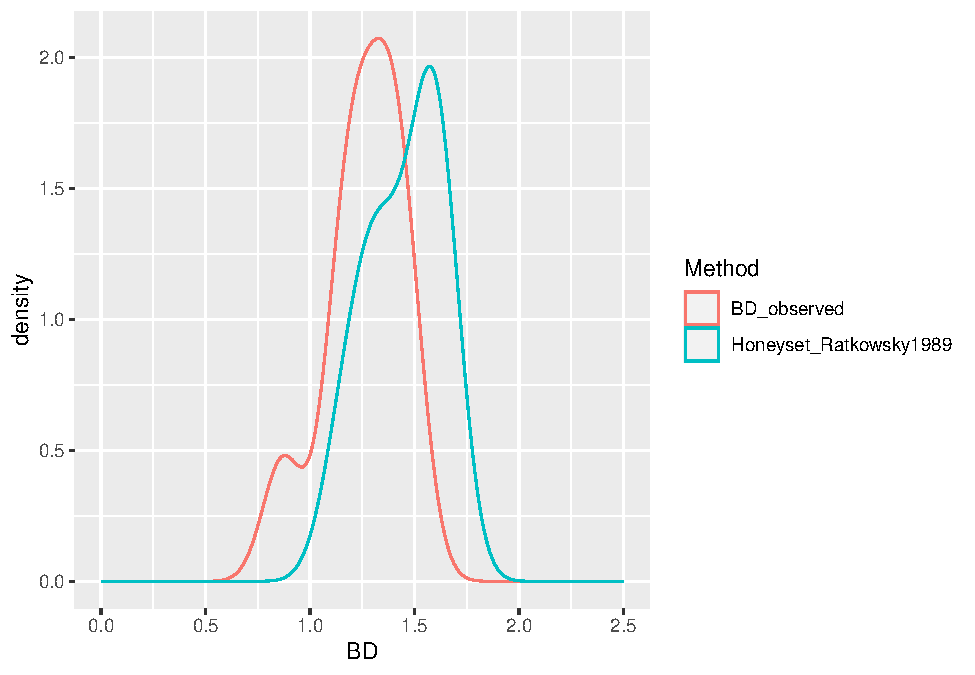
\includegraphics{GSNmap_Technical_Manual_files/figure-latex/unnamed-chunk-11-4.pdf}

\begin{Shaded}
\begin{Highlighting}[]
\CommentTok{\# Same dynamic plot }
\NormalTok{plotly}\SpecialCharTok{::}\FunctionTok{ggplotly}\NormalTok{(BD\_test }\SpecialCharTok{\%\textgreater{}\%} 
           \FunctionTok{select}\NormalTok{(}\SpecialCharTok{{-}}\NormalTok{SOC) }\SpecialCharTok{\%\textgreater{}\%} 
           \FunctionTok{pivot\_longer}\NormalTok{(}\AttributeTok{cols =} \FunctionTok{c}\NormalTok{(}\StringTok{"BD\_observed"}\NormalTok{, }\StringTok{"Honeyset\_Ratkowsky1989"}\NormalTok{), }
                        \AttributeTok{names\_to =} \StringTok{"Method"}\NormalTok{, }\AttributeTok{values\_to =} \StringTok{"BD"}\NormalTok{) }\SpecialCharTok{\%\textgreater{}\%} 
           \FunctionTok{ggplot}\NormalTok{(}\FunctionTok{aes}\NormalTok{(}\AttributeTok{x =}\NormalTok{ BD, }\AttributeTok{color =}\NormalTok{ Method)) }\SpecialCharTok{+} 
           \FunctionTok{geom\_density}\NormalTok{() }\SpecialCharTok{+} \FunctionTok{xlim}\NormalTok{(}\FunctionTok{c}\NormalTok{(}\DecValTok{0}\NormalTok{,}\FloatTok{2.5}\NormalTok{))) }
\end{Highlighting}
\end{Shaded}

The PTF to be chosen for estimating the BD of the missing horizons should be the closest to the measured BD values. Once, the appropriate PTF was chosen, the \texttt{estimateBD} function is applied in the dataframe \texttt{dat} that was created at the end of the quality check. Here, new bd values are estimated for the rows in which the column `bd' has missing values. Finally, a plot is generated to visualize the gap-filled bulk density values.

\begin{Shaded}
\begin{Highlighting}[]
\DocumentationTok{\#\# 5.4 Estimate BD for the missing horizons {-}{-}{-}{-}{-}{-}{-}{-}{-}{-}{-}{-}{-}{-}{-}{-}{-}{-}{-}{-}{-}{-}{-}{-}{-}{-}{-}{-}{-}{-}{-}{-}{-}{-}{-}{-}}
\NormalTok{dat}\SpecialCharTok{$}\NormalTok{bd[}\FunctionTok{is.na}\NormalTok{(dat}\SpecialCharTok{$}\NormalTok{bd)] }\OtherTok{\textless{}{-}}
  \FunctionTok{estimateBD}\NormalTok{(dat[}\FunctionTok{is.na}\NormalTok{(dat}\SpecialCharTok{$}\NormalTok{bd),]}\SpecialCharTok{$}\NormalTok{soc, }\AttributeTok{method=}\StringTok{"Honeyset\_Ratkowsky1989"}\NormalTok{)}

\CommentTok{\# Explore the results}
\FunctionTok{summary}\NormalTok{(dat}\SpecialCharTok{$}\NormalTok{bd)}
\end{Highlighting}
\end{Shaded}

\begin{verbatim}
##    Min. 1st Qu.  Median    Mean 3rd Qu.    Max.    NA's 
##  0.4192  1.2624  1.5797  1.4773  1.7008  1.7670     356
\end{verbatim}

\begin{Shaded}
\begin{Highlighting}[]
\NormalTok{g }\OtherTok{\textless{}{-}}\NormalTok{ BD\_test }\SpecialCharTok{\%\textgreater{}\%} 
  \FunctionTok{select}\NormalTok{(}\SpecialCharTok{{-}}\NormalTok{SOC) }\SpecialCharTok{\%\textgreater{}\%} 
  \FunctionTok{pivot\_longer}\NormalTok{(}\AttributeTok{cols =} \FunctionTok{c}\NormalTok{(}\StringTok{"BD\_observed"}\NormalTok{), }
               \AttributeTok{names\_to =} \StringTok{"Method"}\NormalTok{, }\AttributeTok{values\_to =} \StringTok{"BD"}\NormalTok{) }\SpecialCharTok{\%\textgreater{}\%} 
  \FunctionTok{ggplot}\NormalTok{(}\FunctionTok{aes}\NormalTok{(}\AttributeTok{x =}\NormalTok{ BD, }\AttributeTok{color =}\NormalTok{ Method)) }\SpecialCharTok{+} 
  \FunctionTok{geom\_density}\NormalTok{() }\SpecialCharTok{+}
  \FunctionTok{xlim}\NormalTok{(}\FunctionTok{c}\NormalTok{(}\DecValTok{0}\NormalTok{,}\FloatTok{2.5}\NormalTok{))}
\NormalTok{g }\SpecialCharTok{+} \FunctionTok{geom\_density}\NormalTok{(}\AttributeTok{data =}\NormalTok{ dat, }\FunctionTok{aes}\NormalTok{(}\AttributeTok{x=}\NormalTok{bd, }\AttributeTok{color =} \StringTok{"Predicted +}\SpecialCharTok{\textbackslash{}n}\StringTok{ observed"}\NormalTok{))}
\end{Highlighting}
\end{Shaded}

\begin{verbatim}
## Warning: Removed 356 rows containing non-finite values
## (`stat_density()`).
\end{verbatim}

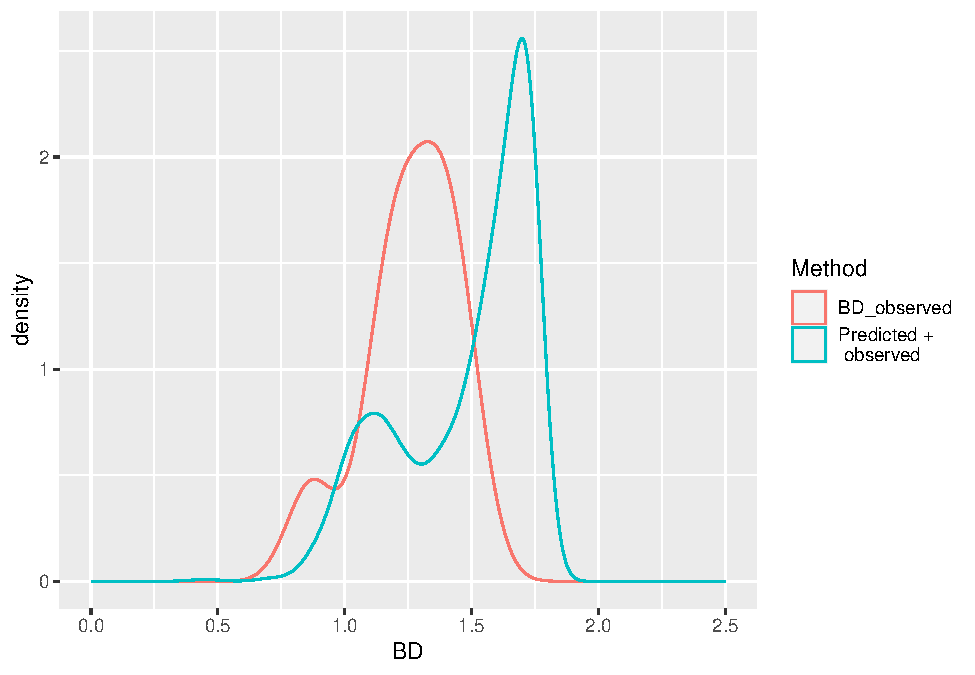
\includegraphics{GSNmap_Technical_Manual_files/figure-latex/unnamed-chunk-12-1.pdf}

\hypertarget{check-for-outliers}{%
\section{Check for outliers}\label{check-for-outliers}}

Unrealistically high or low values can have considerable impact on the statistical analysis and thus it is key to identify and carefully check those values in order to get valid results and eliminate potential bias. Again, the summary() function is apt to show general descriptive statistics such as maxima or minima. Based on this assessment, more detailed views of the suspicious values can be obtained by filtering values above or below a certain threshold as done in the code below for soil organic carbon (SOC) values above 10 percent. If such values don't belong to soil types that would justify such exceptionally high SOC values, e.g.~organic soils (Histosols), these rows can be removed based on the profile ID. The same process should be repeated for all soil properties.
Such evaluation can also be conducted visually for several properties at the same time using the \texttt{tidyverse} and \texttt{ggplot} package that allows to plot boxplots for several soil properties at the same time. To get more information on tidyverse, please follow this link: \url{https://r4ds.had.co.nz/}. For a comprehensive overview of the functionalities of ggplot, a more sophisticated way of plotting, this book provides a good overview: \url{http://www.cookbook-r.com/Graphs/}.

\begin{Shaded}
\begin{Highlighting}[]
\DocumentationTok{\#\# 5.5 {-} Explore outliers {-}{-}{-}{-}{-}{-}{-}{-}{-}{-}{-}{-}{-}{-}{-}{-}{-}{-}{-}{-}{-}{-}{-}{-}{-}{-}{-}{-}{-}{-}{-}{-}{-}{-}{-}{-}{-}{-}{-}{-}{-}{-}{-}{-}{-}{-}{-}{-}{-}{-}{-}{-}{-}{-}}
\CommentTok{\# Outliers should be carefully explored and compared with literature values.}
\CommentTok{\# Only if it is clear that outliers represent impossible or highly unlikely }
\CommentTok{\# values, they should be removed as errors.}
\CommentTok{\# }
\CommentTok{\# Carbon content higher than 15\% is only typical for organic soil (histosols)}
\CommentTok{\# We will remove all atypically high SOC as outliers}
\FunctionTok{summary}\NormalTok{(dat}\SpecialCharTok{$}\NormalTok{soc)}
\end{Highlighting}
\end{Shaded}

\begin{verbatim}
##    Min. 1st Qu.  Median    Mean 3rd Qu.    Max.    NA's 
##   0.020   0.250   0.720   1.451   2.340  19.000     356
\end{verbatim}

\begin{Shaded}
\begin{Highlighting}[]
\FunctionTok{na.omit}\NormalTok{(dat}\SpecialCharTok{$}\NormalTok{ProfID[dat}\SpecialCharTok{$}\NormalTok{soc }\SpecialCharTok{\textgreater{}} \DecValTok{10}\NormalTok{])}
\end{Highlighting}
\end{Shaded}

\begin{verbatim}
## [1] 6915 7726
## attr(,"na.action")
##   [1]   1   2   3   4   5   6   7   8   9  10  11  12  13  14  15  16  17  18
##  [19]  19  20  21  22  23  24  25  26  27  28  29  30  31  32  33  34  35  36
##  [37]  37  38  39  40  41  42  43  44  45  46  47  48  49  50  51  52  53  54
##  [55]  55  56  57  58  59  60  61  62  63  64  65  66  67  68  69  70  71  72
##  [73]  73  74  75  76  77  78  79  80  81  82  83  84  85  86  87  88  89  90
##  [91]  91  92  93  94  95  96  97  98  99 100 101 102 103 104 105 106 107 108
## [109] 109 110 111 112 113 114 115 116 117 118 119 120 121 122 124 125 126 127
## [127] 128 129 130 131 132 133 134 135 136 137 138 139 140 141 142 143 144 145
## [145] 146 147 148 149 150 151 152 153 154 155 156 157 158 159 160 161 162 163
## [163] 164 165 166 167 168 169 170 171 172 173 174 175 176 177 178 179 180 181
## [181] 182 183 184 185 186 187 188 189 190 191 192 193 194 195 196 197 198 199
## [199] 200 201 202 203 204 205 206 207 208 209 210 211 212 213 214 215 216 217
## [217] 218 219 220 221 222 223 224 225 226 227 228 229 230 231 232 233 234 235
## [235] 236 237 238 239 240 241 242 243 244 245 246 247 248 249 250 251 252 253
## [253] 254 255 256 257 258 259 260 261 262 263 264 265 266 267 268 269 270 271
## [271] 272 273 274 275 276 277 278 279 280 281 282 283 284 285 286 287 288 289
## [289] 290 291 292 293 294 295 296 297 298 299 300 301 302 303 304 305 306 307
## [307] 308 309 310 311 312 313 314 315 316 317 318 319 320 321 322 323 324 325
## [325] 326 327 328 329 330 331 332 333 334 335 336 337 339 340 341 342 343 344
## [343] 345 346 347 348 349 350 351 352 353 354 355 356 357 358
## attr(,"class")
## [1] "omit"
\end{verbatim}

\begin{Shaded}
\begin{Highlighting}[]
\NormalTok{dat}\SpecialCharTok{$}\NormalTok{ProfID[dat}\SpecialCharTok{$}\NormalTok{soc }\SpecialCharTok{\textgreater{}} \DecValTok{10}\NormalTok{][}\SpecialCharTok{!}\FunctionTok{is.na}\NormalTok{(dat}\SpecialCharTok{$}\NormalTok{ProfID[dat}\SpecialCharTok{$}\NormalTok{soc }\SpecialCharTok{\textgreater{}} \DecValTok{10}\NormalTok{])] }
\end{Highlighting}
\end{Shaded}

\begin{verbatim}
## [1] 6915 7726
\end{verbatim}

\begin{Shaded}
\begin{Highlighting}[]
\NormalTok{dat }\OtherTok{\textless{}{-}}\NormalTok{ dat[dat}\SpecialCharTok{$}\NormalTok{ProfID }\SpecialCharTok{!=} \DecValTok{6915}\NormalTok{,]}
\NormalTok{dat }\OtherTok{\textless{}{-}}\NormalTok{ dat[dat}\SpecialCharTok{$}\NormalTok{ProfID }\SpecialCharTok{!=} \DecValTok{7726}\NormalTok{,]}

\NormalTok{dat}\OtherTok{\textless{}{-}}\NormalTok{ dat[}\SpecialCharTok{!}\NormalTok{(dat}\SpecialCharTok{$}\NormalTok{ProfID }\SpecialCharTok{\%in\%}\NormalTok{ dat}\SpecialCharTok{$}\NormalTok{ProfID[dat}\SpecialCharTok{$}\NormalTok{soc }\SpecialCharTok{\textgreater{}} \DecValTok{10}\NormalTok{][}\SpecialCharTok{!}\FunctionTok{is.na}\NormalTok{(dat}\SpecialCharTok{$}\NormalTok{ProfID[dat}\SpecialCharTok{$}\NormalTok{soc }\SpecialCharTok{\textgreater{}} \DecValTok{10}\NormalTok{])]),]}

\CommentTok{\# Explore bulk density data, identify outliers}
\CommentTok{\# remove layers with Bulk Density \textless{} 1 g/cm\^{}3}
\NormalTok{low\_bd\_profiles }\OtherTok{\textless{}{-}} \FunctionTok{na.omit}\NormalTok{(dat}\SpecialCharTok{$}\NormalTok{ProfID[dat}\SpecialCharTok{$}\NormalTok{bd}\SpecialCharTok{\textless{}}\DecValTok{1}\NormalTok{])}
\NormalTok{dat }\OtherTok{\textless{}{-}}\NormalTok{ dat[}\SpecialCharTok{!}\NormalTok{(dat}\SpecialCharTok{$}\NormalTok{ProfID }\SpecialCharTok{\%in\%}\NormalTok{ low\_bd\_profiles),]}

\CommentTok{\# Explore data, identify outliers}
\NormalTok{x }\OtherTok{\textless{}{-}} \FunctionTok{pivot\_longer}\NormalTok{(dat, }\AttributeTok{cols =}\NormalTok{ ph}\SpecialCharTok{:}\NormalTok{cec, }\AttributeTok{values\_to =} \StringTok{"value"}\NormalTok{,}
                  \AttributeTok{names\_to =} \StringTok{"soil\_property"}\NormalTok{)}
\NormalTok{x }\OtherTok{\textless{}{-}} \FunctionTok{na.omit}\NormalTok{(x)}
\FunctionTok{ggplot}\NormalTok{(x, }\FunctionTok{aes}\NormalTok{(}\AttributeTok{x =}\NormalTok{ soil\_property, }\AttributeTok{y =}\NormalTok{ value, }\AttributeTok{fill =}\NormalTok{ soil\_property)) }\SpecialCharTok{+}
  \FunctionTok{geom\_boxplot}\NormalTok{() }\SpecialCharTok{+} 
  \FunctionTok{facet\_wrap}\NormalTok{(}\SpecialCharTok{\textasciitilde{}}\NormalTok{soil\_property, }\AttributeTok{scales =} \StringTok{"free"}\NormalTok{)}
\end{Highlighting}
\end{Shaded}

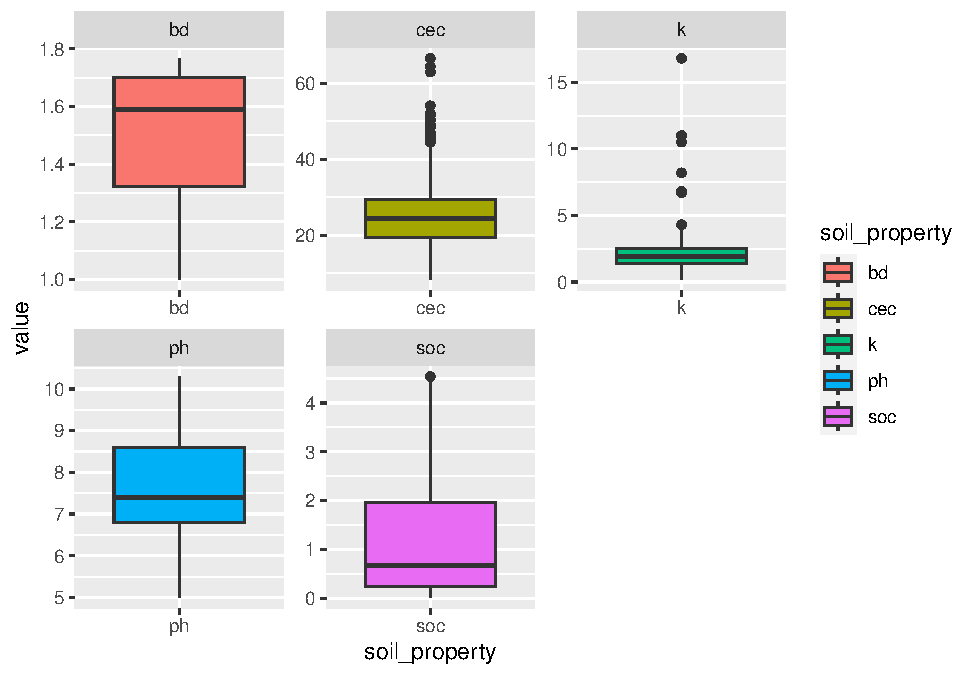
\includegraphics{GSNmap_Technical_Manual_files/figure-latex/unnamed-chunk-13-1.pdf}

\hypertarget{harmonise-soil-layer-depths}{%
\section{Harmonise soil layer depths}\label{harmonise-soil-layer-depths}}

The last step towards a soil data table that can be used for mapping, is to harmonize the soil depth layers to 0-30 cm (or 30-60, or 60-100 cm respectively). This is necessary since we want to produce maps that cover exactly those depths and do not differ across soil profile locations. Thus, the relevant columns are selected from the dataframe, target soil properties, and upper and lower limit of the harmonised soil layer are specified (in depths).

In the following a new dataframe `d' is created in which the standard depth layers are stored and named. To achieve this the function apply\_mpspline\_all from mpslpine2 is used.

\begin{Shaded}
\begin{Highlighting}[]
\CommentTok{\# 6 {-} Harmonize soil layers ====================================================}
\FunctionTok{source}\NormalTok{(}\StringTok{"Digital{-}Soil{-}Mapping/03{-}Scripts/spline\_functions.R"}\NormalTok{) }
\DocumentationTok{\#\# 6.1 {-} Set target soil properties and depths {-}{-}{-}{-}{-}{-}{-}{-}{-}{-}{-}{-}{-}{-}{-}{-}{-}{-}{-}{-}{-}{-}{-}{-}{-}{-}{-}{-}{-}{-}{-}{-}{-}}
\FunctionTok{names}\NormalTok{(dat)}
\NormalTok{dat }\OtherTok{\textless{}{-}} \FunctionTok{select}\NormalTok{(dat, ProfID, HorID, x, y, top, bottom, ph, k, soc, bd, cec)}

\NormalTok{target }\OtherTok{\textless{}{-}} \FunctionTok{c}\NormalTok{(}\StringTok{"ph"}\NormalTok{, }\StringTok{"k"}\NormalTok{, }\StringTok{"soc"}\NormalTok{,  }\StringTok{"bd"}\NormalTok{, }\StringTok{"cec"}\NormalTok{)}
\NormalTok{depths }\OtherTok{\textless{}{-}} \FunctionTok{c}\NormalTok{(}\DecValTok{0}\NormalTok{,}\DecValTok{30}\NormalTok{)}

\DocumentationTok{\#\# 6.2 {-} Create standard layers {-}{-}{-}{-}{-}{-}{-}{-}{-}{-}{-}{-}{-}{-}{-}{-}{-}{-}{-}{-}{-}{-}{-}{-}{-}{-}{-}{-}{-}{-}{-}{-}{-}{-}{-}{-}{-}{-}{-}{-}{-}{-}{-}{-}{-}{-}{-}{-}}
\NormalTok{splines }\OtherTok{\textless{}{-}}\FunctionTok{apply\_mpspline\_all}\NormalTok{(}\AttributeTok{df =}\NormalTok{ dat, }\AttributeTok{properties =}\NormalTok{ target, }\AttributeTok{depth\_range =}\NormalTok{ depths)}
\FunctionTok{summary}\NormalTok{(splines)}

\CommentTok{\# merge splines with x and y}
\NormalTok{d }\OtherTok{\textless{}{-}} \FunctionTok{unique}\NormalTok{(}\FunctionTok{select}\NormalTok{(dat, ProfID, x, y))}
\NormalTok{d }\OtherTok{\textless{}{-}} \FunctionTok{left\_join}\NormalTok{(d, splines)}
\end{Highlighting}
\end{Shaded}

\hypertarget{harmonise-units}{%
\section{Harmonise units}\label{harmonise-units}}

Units are of paramount importance to deliver a high-quality map product. Therefore, special attention needs to be paid to a correct conversion/harmonisation of units particularly if different spreadsheets are combined. The mandatory soil properties need to be delivered in the following units:

\begin{Shaded}
\begin{Highlighting}[]
\CommentTok{\# 7 {-} Harmonise units ==========================================================}
\CommentTok{\#Harmonise units if different from target units}
\CommentTok{\# Mandatory Soil Properties and corresponding units:}
\CommentTok{\# Total N {-} ppm}
\CommentTok{\# Available P {-} ppm}
\CommentTok{\# Available K {-} ppm}
\CommentTok{\# Cation exchange capacity cmolc/kg}
\CommentTok{\# pH}
\CommentTok{\# SOC {-} \%}
\CommentTok{\# Bulk density g/cm3}
\CommentTok{\# Soil fractions (clay, silt and sand) {-} }
\end{Highlighting}
\end{Shaded}

In the following, the available Potassium measurements from the soil profile data is converted from cmol\textsubscript{c}/kg to ppm. In addition, total N is converted from percent to ppm and the soil texture class values from g/kg to percent.

\begin{Shaded}
\begin{Highlighting}[]
\CommentTok{\# Units soil profile data (dataframe d)}
\CommentTok{\# }
\FunctionTok{head}\NormalTok{(d) }\CommentTok{\# pH; K cmolc/kg; SOC \%; BD g/cm3; CEC  cmolc/kg}

\CommentTok{\# K =\textgreater{} convert cmolc/kg to ppm (K *10 * 39.096)}
\NormalTok{d}\SpecialCharTok{$}\NormalTok{k\_0\_30 }\OtherTok{\textless{}{-}}\NormalTok{ d}\SpecialCharTok{$}\NormalTok{k\_0\_30}\SpecialCharTok{*}\DecValTok{10} \SpecialCharTok{*} \FloatTok{39.096}

\FunctionTok{head}\NormalTok{(chem)}\CommentTok{\# P ppm; N \%; K ppm}
\CommentTok{\# N =\textgreater{} convert \% to ppm (N * 10000)}
\NormalTok{chem}\SpecialCharTok{$}\NormalTok{tn }\OtherTok{\textless{}{-}}\NormalTok{chem}\SpecialCharTok{$}\NormalTok{tn}\SpecialCharTok{*}\DecValTok{10000}

\FunctionTok{head}\NormalTok{(phys)}\CommentTok{\# clay, sand, silt g/kg}
\CommentTok{\# convert g/kg to \% (/10)}
\NormalTok{phys}\SpecialCharTok{$}\NormalTok{clay\_0\_30 }\OtherTok{\textless{}{-}}\NormalTok{phys}\SpecialCharTok{$}\NormalTok{clay\_0\_30}\SpecialCharTok{/}\DecValTok{10}
\NormalTok{phys}\SpecialCharTok{$}\NormalTok{sand\_0\_30  }\OtherTok{\textless{}{-}}\NormalTok{phys}\SpecialCharTok{$}\NormalTok{sand\_0\_30 }\SpecialCharTok{/}\DecValTok{10}
\NormalTok{phys}\SpecialCharTok{$}\NormalTok{silt\_0\_30 }\OtherTok{\textless{}{-}}\NormalTok{phys}\SpecialCharTok{$}\NormalTok{silt\_0\_30}\SpecialCharTok{/}\DecValTok{10}
\end{Highlighting}
\end{Shaded}

Finally, the different spreadsheets are merged into one single dataframe. For that, it is important to have matching column names in the dataframes that are to be merged.

\begin{Shaded}
\begin{Highlighting}[]
\CommentTok{\# Add chemical and physical properties from additional datasets ==========================}
  

\CommentTok{\# Rename columns to match the main data set}
\FunctionTok{names}\NormalTok{(d)}
\FunctionTok{names}\NormalTok{(chem)[}\DecValTok{1}\NormalTok{] }\OtherTok{\textless{}{-}} \StringTok{\textquotesingle{}ProfID\textquotesingle{}}
\FunctionTok{names}\NormalTok{(chem)[}\DecValTok{4}\NormalTok{] }\OtherTok{\textless{}{-}} \StringTok{\textquotesingle{}p\_0\_30\textquotesingle{}}
\FunctionTok{names}\NormalTok{(chem)[}\DecValTok{5}\NormalTok{] }\OtherTok{\textless{}{-}} \StringTok{\textquotesingle{}k\_0\_30\textquotesingle{}} 
\FunctionTok{names}\NormalTok{(chem)[}\DecValTok{6}\NormalTok{] }\OtherTok{\textless{}{-}} \StringTok{\textquotesingle{}n\_0\_30\textquotesingle{}}


\CommentTok{\#The chem dataframe comes from and independent dataset we need to create new unique ProfIDs }
\CommentTok{\#Create unique ProfID }
\NormalTok{chem}\SpecialCharTok{$}\NormalTok{ProfID }\OtherTok{\textless{}{-}} \FunctionTok{seq}\NormalTok{(}\FunctionTok{max}\NormalTok{(d}\SpecialCharTok{$}\NormalTok{ProfID)}\SpecialCharTok{+}\DecValTok{1}\NormalTok{,}\FunctionTok{max}\NormalTok{(d}\SpecialCharTok{$}\NormalTok{ProfID)}\SpecialCharTok{+}\DecValTok{1}\SpecialCharTok{+}\FunctionTok{nrow}\NormalTok{(chem)}\SpecialCharTok{{-}}\DecValTok{1}\NormalTok{)}

\CommentTok{\# Add the new data as new rows using dplyr we can add empty rows}
\CommentTok{\# automatically for the not measured properties in the chem dataset}
\NormalTok{d }\OtherTok{\textless{}{-}} \FunctionTok{bind\_rows}\NormalTok{(d, chem)}

\CommentTok{\#The phys dataframe with the texture instead shares the same ProfIDs (we can directly merge)}
\NormalTok{d }\OtherTok{\textless{}{-}} \FunctionTok{left\_join}\NormalTok{(d, phys, }\AttributeTok{by=}\FunctionTok{c}\NormalTok{(}\StringTok{\textquotesingle{}ProfID\textquotesingle{}}\NormalTok{, }\StringTok{\textquotesingle{}x\textquotesingle{}}\NormalTok{, }\StringTok{\textquotesingle{}y\textquotesingle{}}\NormalTok{))}
\end{Highlighting}
\end{Shaded}

\hypertarget{save-the-results}{%
\section{Save the results}\label{save-the-results}}

Before finalising the soil data preparation, it is recommendable to check again visually if the calculations were conducted correctly. Again, the combination of tidyverse and ggplot functions provides high efficiency and versatility to visualise figures with the desired soil properties. At last, the write\_csv() function is used to save the dataframe as a .csv file in the Outputs folder (02-Outputs). With this, the soil data preparation is finalised.

\begin{Shaded}
\begin{Highlighting}[]
\CommentTok{\# 8 {-} Plot  and save results ===================================================}
\FunctionTok{names}\NormalTok{(d)}
\NormalTok{x }\OtherTok{\textless{}{-}} \FunctionTok{pivot\_longer}\NormalTok{(d, }\AttributeTok{cols =}\NormalTok{ ph\_0\_30}\SpecialCharTok{:}\NormalTok{silt\_0\_30, }\AttributeTok{values\_to =} \StringTok{"value"}\NormalTok{,}
                  \AttributeTok{names\_sep =} \StringTok{"\_"}\NormalTok{, }
                  \AttributeTok{names\_to =} \FunctionTok{c}\NormalTok{(}\StringTok{"soil\_property"}\NormalTok{, }\StringTok{"top"}\NormalTok{, }\StringTok{"bottom"}\NormalTok{))}
\NormalTok{x }\OtherTok{\textless{}{-}} \FunctionTok{mutate}\NormalTok{(x, }\AttributeTok{depth =} \FunctionTok{paste}\NormalTok{(top, }\StringTok{"{-}"}\NormalTok{ , bottom))}
\CommentTok{\#x \textless{}{-} na.omit(x)}
\FunctionTok{ggplot}\NormalTok{(x, }\FunctionTok{aes}\NormalTok{(}\AttributeTok{x =}\NormalTok{ depth, }\AttributeTok{y =}\NormalTok{ value, }\AttributeTok{fill =}\NormalTok{ soil\_property)) }\SpecialCharTok{+}
  \FunctionTok{geom\_boxplot}\NormalTok{() }\SpecialCharTok{+} 
  \FunctionTok{facet\_wrap}\NormalTok{(}\SpecialCharTok{\textasciitilde{}}\NormalTok{soil\_property, }\AttributeTok{scales =} \StringTok{"free"}\NormalTok{)}


\NormalTok{plotly}\SpecialCharTok{::}\FunctionTok{ggplotly}\NormalTok{(}\FunctionTok{ggplot}\NormalTok{(x, }\FunctionTok{aes}\NormalTok{(}\AttributeTok{x =}\NormalTok{ depth, }\AttributeTok{y =}\NormalTok{ value, }\AttributeTok{fill =}\NormalTok{ soil\_property)) }\SpecialCharTok{+}
           \FunctionTok{geom\_boxplot}\NormalTok{() }\SpecialCharTok{+} 
           \FunctionTok{facet\_wrap}\NormalTok{(}\SpecialCharTok{\textasciitilde{}}\NormalTok{soil\_property, }\AttributeTok{scales =} \StringTok{"free"}\NormalTok{))}

\CommentTok{\# save the data}
\FunctionTok{write\_csv}\NormalTok{(d, }\StringTok{"02{-}Outputs/harmonized\_soil\_data.csv"}\NormalTok{)}
\end{Highlighting}
\end{Shaded}

\hypertarget{step-2-download-environmental-covariates}{%
\chapter{Step 2: download environmental covariates}\label{step-2-download-environmental-covariates}}

\hypertarget{environmental-covariates}{%
\section{Environmental covariates}\label{environmental-covariates}}

The SCORPAN equation (Eq. \eqref{eq:scorpan}) refers to the soil-forming factors that determine the spatial variation of soils. However, these factors cannot be measured directly. Instead, proxies of these soil forming factors are used. One essential characteristic of the environmental covariates is that they are spatially explicit, covering the whole study area. The following Table \ref{tab:covs1} lists all the environmental covariates that can be implemented under the present DSM framework. Apart from the environmental covariates mentioned in Table \ref{tab:covs1}, other types of maps could also be included, such as Global Surface Water Mapping Layers and Water Soil Erosion from the Joint Research Centre (JRC). At national level there may be very significant covariates that could complement or replace the covariates of Table \ref{tab:covs1}. Thus, the selection of suitable covariate layers needs to be assessed with common sense and applying expert knowledge.

\begingroup\fontsize{7}{9}\selectfont

\begin{longtable}[t]{lll}
\caption{\label{tab:covs1}List of environmental covariates.}\\
\toprule
Description & Code & Resolution  m \\
\midrule
\endfirsthead
\caption[]{\label{tab:covs1}List of environmental covariates. }\\
\toprule
Description & Code & Resolution  m \\
\midrule
\endhead

\endfoot
\bottomrule
\endlastfoot
\addlinespace[0.3em]
\multicolumn{3}{l}{\textbf{Temperature}}\\
\hspace{1em}Mean air temperature (annual) & bio1 & 1000\\
\hspace{1em}Mean daily temperature of warmest month & bio5 & 1000\\
\hspace{1em}Mean daily temperature of coldest month & bio6 & 1000\\
\addlinespace[0.3em]
\multicolumn{3}{l}{\textbf{Precipitation}}\\
\hspace{1em}Mean annual precipitation & bio12 & 1000\\
\hspace{1em}Mean precipitation of wettest month & bio13 & 1000\\
\hspace{1em}Mean precipitation of driest month & bio14 & 1000\\
\hspace{1em}Mean monthly precipitation of wettest quarter & bio16 & 1000\\
\hspace{1em}Mean monthly precipitation of driest quarter & bio17 & 1000\\
\addlinespace[0.3em]
\multicolumn{3}{l}{\textbf{Potential evapotranspiration (PET)}}\\
\hspace{1em}Mean monthly PET & pet\_penman\_mean & 1000\\
\hspace{1em}Minimum monthly PET & pet\_penman\_min & 1000\\
\hspace{1em}Range monthly PET & pet\_penman\_range & 1000\\
\hspace{1em}Maximum monthly PET & pet\_penman\_max & 1000\\
\addlinespace[0.3em]
\multicolumn{3}{l}{\textbf{Wind}}\\
\hspace{1em}Minimum monthly wind speed & sfcWind\_min & 1000\\
\hspace{1em}Maximum monthly wind speed & sfcWind\_max & 1000\\
\hspace{1em}Range monthly wind speed & sfcWind\_range & 1000\\
\addlinespace[0.3em]
\multicolumn{3}{l}{\textbf{Growing season}}\\
\hspace{1em}Number of days with mean daily air & ngd10 & 1000\\
\hspace{1em}temperature above 10 degrees Celsius &  & \\
\addlinespace[0.3em]
\multicolumn{3}{l}{\textbf{Vegetation indices (NDVI) (MOD13Q1)}}\\
\hspace{1em}Mean March-May from 2000-2022 & ndvi\_030405\_mean & 250\\
\hspace{1em}Mean June-August from 2000-2022 & ndvi\_060708\_mean & 250\\
\hspace{1em}Mean September-November from 2000-2022 & ndvi\_091011\_mean & 250\\
\hspace{1em}Mean December-February from 2000-2022 & ndvi\_120102\_mean & 250\\
\hspace{1em}Standard deviation March-May (2000-2022) & ndvi\_030405\_sd & 250\\
\hspace{1em}Standard deviation June-August (2000-2022) & ndvi\_060708\_sd & 250\\
\hspace{1em}Standard deviation Sept.-Nov. (2000-2022) & ndvi\_091011\_sd & 250\\
\hspace{1em}Standard deviation Dec.-Feb. (2000-2022) & ndvi\_120102\_sd & 250\\
\addlinespace[0.3em]
\multicolumn{3}{l}{\textbf{Fraction of photosynthetically active radiation (FPAR) (MOD15A2H)}}\\
\hspace{1em}Mean March-May from 2000-2022 & fpar\_030405\_mean & 500\\
\hspace{1em}Mean June-August from 2000-2022 & fpar\_060708\_mean & 500\\
\hspace{1em}Mean September-November from 2000-2022 & fpar\_091011\_mean & 500\\
\hspace{1em}Mean December-February from 2000-2022 & fpar\_120102\_mean & 500\\
\hspace{1em}Standard deviation March-May (2000-2022) & fpar\_030405\_sd & 500\\
\hspace{1em}Standard deviation June-August (2000-2022) & fpar\_060708\_sd & 500\\
\hspace{1em}Standard deviation Sept.-Nov. (2000-2022) & fpar\_091011\_sd & 500\\
\hspace{1em}Standard deviation Dec.-Feb. (2000-2022) & fpar\_120102\_sd & 500\\
\addlinespace[0.3em]
\multicolumn{3}{l}{\textbf{Land surface temperature day (LSTD) (MOD11A2)}}\\
\hspace{1em}Mean March-May from 2000-2022 & lstd\_030405\_mean & 1000\\
\hspace{1em}Mean June-August from 2000-2022 & lstd\_060708\_mean & 1000\\
\hspace{1em}Mean September-November from 2000-2022 & lstd\_091011\_mean & 1000\\
\hspace{1em}Mean December-February from 2000-2022 & lstd\_120102\_mean & 1000\\
\hspace{1em}Standard deviation March-May (2000-2022) & lstd\_030405\_sd & 1000\\
\hspace{1em}Standard deviation June-August (2000-2022) & lstd\_060708\_sd & 1000\\
\hspace{1em}Standard deviation Sept.-Nov. (2000-2022) & lstd\_091011\_sd & 1000\\
\hspace{1em}Standard deviation Dec.-Feb. (2000-2022) & lstd\_120102\_sd & 1000\\
\addlinespace[0.3em]
\multicolumn{3}{l}{\textbf{Normalised difference between LST day and LST night (MOD11A2)}}\\
\hspace{1em}Mean March-May from 2000-2022 & ndlstd\_030405\_mean & 1000\\
\hspace{1em}Mean June-August from 2000-2022 & ndlstd\_060708\_mean & 1000\\
\hspace{1em}Mean September-November from 2000-2022 & ndlstd\_091011\_mean & 1000\\
\hspace{1em}Mean December-February from 2000-2022 & ndlstd\_120102\_mean & 1000\\
\hspace{1em}Standard deviation March-May (2000-2022) & ndlstd\_030405\_sd & 1000\\
\hspace{1em}Standard deviation June-August (2000-2022) & ndlstd\_060708\_sd & 1000\\
\hspace{1em}Standard deviation Sept.-Nov. (2000-2022) & ndlstd\_091011\_sd & 1000\\
\hspace{1em}Standard deviation Dec.-Feb. (2000-2022) & ndlstd\_120102\_sd & 1000\\
\addlinespace[0.3em]
\multicolumn{3}{l}{\textbf{Short-wave Infrared (SWIR) black-sky albedo for shortwave broadband (MCD43A3)}}\\
\hspace{1em}Mean June-August from 2000-2022 & swir\_060708\_mean & 5--\\
\addlinespace[0.3em]
\multicolumn{3}{l}{\textbf{MODIS snow cover (MOD10A1)}}\\
\hspace{1em}Mean snow cover & mean\_snow\_cover & 500\\
\addlinespace[0.3em]
\multicolumn{3}{l}{\textbf{Land cover dynamic world 10m near real-time land use/land cover (LULC) dataset}}\\
\hspace{1em}Mean estimated probability of complete coverage by trees & trees & 250\\
\hspace{1em}Mean estimated probability of complete coverage & shrub\_and\_scrub & 250\\
\hspace{1em}by shrub and scrub &  & \\
\hspace{1em}Mean estimated probability of complete coverage & flooded\_vegetation & 250\\
\hspace{1em}by flooded vegetation &  & \\
\hspace{1em}Mean estimated probability of complete coverage & grass & 250\\
\hspace{1em}by grasses &  & \\
\hspace{1em}Mean estimated probability of complete coverage & crop & 250\\
\hspace{1em}by bare &  & \\
\addlinespace[0.3em]
\multicolumn{3}{l}{\textbf{Terrain}}\\
\hspace{1em}Profile curvature & curvature & 250\\
\hspace{1em}Downslope curvature & downslopecurvature & 250\\
\hspace{1em}Upslope curvature & upslopecurvature & 250\\
\hspace{1em}Deviation from mean value & dvm & 250\\
\hspace{1em}deviation from mean value & dvm2 & 250\\
\hspace{1em}Elevation & elevation & 250\\
\hspace{1em}Melton ruggedness number & mrn & 250\\
\hspace{1em}Negative openness & neg\_openness & 250\\
\hspace{1em}Positive openness & pos\_openness & 250\\
\hspace{1em}Slope & slope & 250\\
\hspace{1em}Topographic position index & tpi & 250\\
\hspace{1em}Terrain wetness index & twi & 250\\
\hspace{1em}Multiresolution of valley bottom flatness & vbf & 250\\
Global terrestrial Human Footprint dataset from 2013 & hfp2013\_merisINT & 1000\\
DMSP-OLS Nighttime Lights Time Series & night\_lights\_stable\_2013 & 1000\\
Global Human Settlement Layer 2020 & population\_density\_2020 & 1000\\*
\end{longtable}
\endgroup{}

\hypertarget{download-covariates-and-cropland-mask-with-google-earth-engine-gee}{%
\section{Download covariates and cropland mask with Google Earth Engine (GEE)}\label{download-covariates-and-cropland-mask-with-google-earth-engine-gee}}

The following are the steps to access and download the environmental covariates and cropland mask. The GSP has streamlined the process of downloading environmental covariates clipped to national borders from GEE. This chapter aims to guide you on how to download environmental covariates using a GEE script written in JavaScript.

You can find the JavaScript code in the material provided in this technical manual under \href{https://github.com/FAO-GSP/GSNmap-TM/tree/main/Digital-Soil-Mapping/03-Scripts}{03-scripts/3.0.Download\_Covariates\_\&\_Mask.txt}. To use the code, simply copy and paste the text in the GEE console as shown in the figure below.

\begin{figure}
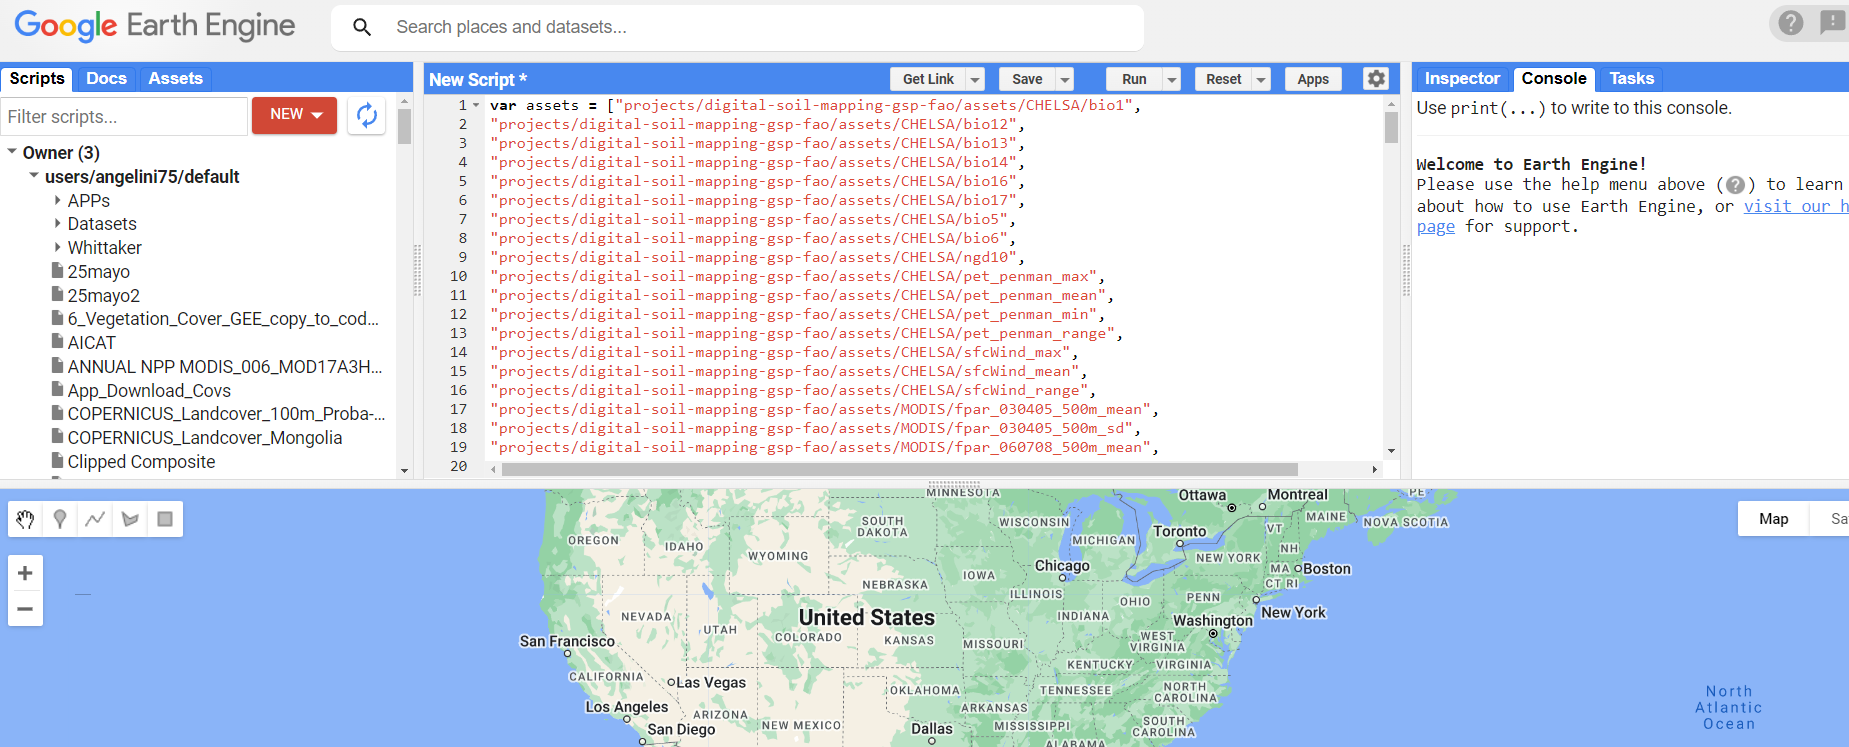
\includegraphics[width=1\linewidth]{images/javaScript_GEE} \caption{Copy and paste script in the code editor.}\label{fig:screenshot}
\end{figure}

If not done already, it is necessary to specify the working directory and a file path directory to the output folder where the clipped covariate layers are going to be saved. In case users want to use their own shapefile of the AOI, it is necessary to specify the file path to load it into our \textbf{R} session later. Alternatively, the shapefile of the AOI can be clipped from the official UN map shapefile that is available in the ``Digital-Soil-Mapping-GSP-FAO'' based on the 3-digit ISO code (ISO3CD column in the attribute table). The process to do this will be explained in a few steps. Finally, it is also necessary to specify the resolution to 250 x 250 m for the covariate layers and set the CRS to WGS84 (equals EPSG code 4326). Note that the target resolution of the GSNmap is at 250 m, which can be considered a moderate resolution for a global layer. However, those countries that require a higher resolution are free to develop higher resolution maps and aggregate the resulting maps to the target resolution of GSNmap for submission.

The following text explains the structure of the script that will be executed in GEE, and which parts of the script need to be modified to extract the covariates from the area of interest (AOI).

\hypertarget{assets}{%
\subsection{Assets}\label{assets}}

In GEE, an ``asset'' refers to any data or code that has been uploaded and stored in GEE's cloud-based servers. Assets can include remote sensing data, vector data, and even scripts or functions.

The following code reads the assets that have been created by the GSP in GEE. This means that the code accesses the data and scripts that GSP has uploaded to GEE, and uses them to perform specific tasks or analyses. By leveraging GEE's cloud-based infrastructure and GSP's assets, users can easily access and analyze large amounts of data without the need for local storage or processing power.

\begin{Shaded}
\begin{Highlighting}[]
\NormalTok{\#Empty environment and cache}
\KeywordTok{var}\NormalTok{ assets }\OperatorTok{=}\NormalTok{ [}\StringTok{"projects/digital{-}soil{-}mapping{-}gsp{-}fao/assets/CHELSA/bio1"}\OperatorTok{,}
\StringTok{"projects/digital{-}soil{-}mapping{-}gsp{-}fao/assets/CHELSA/bio12"}\OperatorTok{,}
\StringTok{"projects/digital{-}soil{-}mapping{-}gsp{-}fao/assets/CHELSA/bio13"}\OperatorTok{,}
\StringTok{"projects/digital{-}soil{-}mapping{-}gsp{-}fao/assets/CHELSA/bio14"}\OperatorTok{,}
\StringTok{"projects/digital{-}soil{-}mapping{-}gsp{-}fao/assets/CHELSA/bio16"}\OperatorTok{,}
\StringTok{"projects/digital{-}soil{-}mapping{-}gsp{-}fao/assets/CHELSA/bio17"}\OperatorTok{,}
\StringTok{"projects/digital{-}soil{-}mapping{-}gsp{-}fao/assets/CHELSA/bio5"}\OperatorTok{,}
\StringTok{"projects/digital{-}soil{-}mapping{-}gsp{-}fao/assets/CHELSA/bio6"}\OperatorTok{,}
\StringTok{"projects/digital{-}soil{-}mapping{-}gsp{-}fao/assets/CHELSA/ngd10"}\OperatorTok{,}
\StringTok{"projects/digital{-}soil{-}mapping{-}gsp{-}fao/assets/CHELSA/pet\_penman\_max"}\OperatorTok{,}
\StringTok{"projects/digital{-}soil{-}mapping{-}gsp{-}fao/assets/CHELSA/pet\_penman\_mean"}\OperatorTok{,}
\StringTok{"projects/digital{-}soil{-}mapping{-}gsp{-}fao/assets/CHELSA/pet\_penman\_min"}\OperatorTok{,}
\StringTok{"projects/digital{-}soil{-}mapping{-}gsp{-}fao/assets/CHELSA/pet\_penman\_range"}\OperatorTok{,}
\StringTok{"projects/digital{-}soil{-}mapping{-}gsp{-}fao/assets/CHELSA/sfcWind\_max"}\OperatorTok{,}
\StringTok{"projects/digital{-}soil{-}mapping{-}gsp{-}fao/assets/CHELSA/sfcWind\_mean"}\OperatorTok{,}
\StringTok{"projects/digital{-}soil{-}mapping{-}gsp{-}fao/assets/CHELSA/sfcWind\_range"}\OperatorTok{,}
\StringTok{"projects/digital{-}soil{-}mapping{-}gsp{-}fao/assets/MODIS/fpar\_030405\_500m\_mean"}\OperatorTok{,}
\StringTok{"projects/digital{-}soil{-}mapping{-}gsp{-}fao/assets/MODIS/fpar\_030405\_500m\_sd"}\OperatorTok{,}
\StringTok{"projects/digital{-}soil{-}mapping{-}gsp{-}fao/assets/MODIS/fpar\_060708\_500m\_mean"}\OperatorTok{,}
\StringTok{"projects/digital{-}soil{-}mapping{-}gsp{-}fao/assets/MODIS/fpar\_060708\_500m\_sd"}\OperatorTok{,}
\StringTok{"projects/digital{-}soil{-}mapping{-}gsp{-}fao/assets/MODIS/fpar\_091011\_500m\_mean"}\OperatorTok{,}
\StringTok{"projects/digital{-}soil{-}mapping{-}gsp{-}fao/assets/MODIS/fpar\_091011\_500m\_sd"}\OperatorTok{,}
\StringTok{"projects/digital{-}soil{-}mapping{-}gsp{-}fao/assets/MODIS/fpar\_120102\_500m\_mean"}\OperatorTok{,}
\StringTok{"projects/digital{-}soil{-}mapping{-}gsp{-}fao/assets/MODIS/fpar\_120102\_500m\_sd"}\OperatorTok{,}
\StringTok{"projects/digital{-}soil{-}mapping{-}gsp{-}fao/assets/MODIS/lstd\_030405\_mean"}\OperatorTok{,}
\StringTok{"projects/digital{-}soil{-}mapping{-}gsp{-}fao/assets/MODIS/lstd\_030405\_sd"}\OperatorTok{,}
\StringTok{"projects/digital{-}soil{-}mapping{-}gsp{-}fao/assets/MODIS/lstd\_060708\_mean"}\OperatorTok{,}
\StringTok{"projects/digital{-}soil{-}mapping{-}gsp{-}fao/assets/MODIS/lstd\_060708\_sd"}\OperatorTok{,}
\StringTok{"projects/digital{-}soil{-}mapping{-}gsp{-}fao/assets/MODIS/lstd\_091011\_mean"}\OperatorTok{,}
\StringTok{"projects/digital{-}soil{-}mapping{-}gsp{-}fao/assets/MODIS/lstd\_091011\_sd"}\OperatorTok{,}
\StringTok{"projects/digital{-}soil{-}mapping{-}gsp{-}fao/assets/MODIS/lstd\_120102\_mean"}\OperatorTok{,}
\StringTok{"projects/digital{-}soil{-}mapping{-}gsp{-}fao/assets/MODIS/lstd\_120102\_sd"}\OperatorTok{,}
\StringTok{"projects/digital{-}soil{-}mapping{-}gsp{-}fao/assets/MODIS/ndlst\_030405\_mean"}\OperatorTok{,}
\StringTok{"projects/digital{-}soil{-}mapping{-}gsp{-}fao/assets/MODIS/ndlst\_030405\_sd"}\OperatorTok{,}
\StringTok{"projects/digital{-}soil{-}mapping{-}gsp{-}fao/assets/MODIS/ndlst\_060708\_mean"}\OperatorTok{,}
\StringTok{"projects/digital{-}soil{-}mapping{-}gsp{-}fao/assets/MODIS/ndlst\_060708\_sd"}\OperatorTok{,}
\StringTok{"projects/digital{-}soil{-}mapping{-}gsp{-}fao/assets/MODIS/ndlst\_091011\_mean"}\OperatorTok{,}
\StringTok{"projects/digital{-}soil{-}mapping{-}gsp{-}fao/assets/MODIS/ndlst\_091011\_sd"}\OperatorTok{,}
\StringTok{"projects/digital{-}soil{-}mapping{-}gsp{-}fao/assets/MODIS/ndlst\_120102\_mean"}\OperatorTok{,}
\StringTok{"projects/digital{-}soil{-}mapping{-}gsp{-}fao/assets/MODIS/ndlst\_120102\_sd"}\OperatorTok{,}
\StringTok{"projects/digital{-}soil{-}mapping{-}gsp{-}fao/assets/MODIS/ndvi\_030405\_250m\_mean"}\OperatorTok{,}
\StringTok{"projects/digital{-}soil{-}mapping{-}gsp{-}fao/assets/MODIS/ndvi\_030405\_250m\_sd"}\OperatorTok{,}
\StringTok{"projects/digital{-}soil{-}mapping{-}gsp{-}fao/assets/MODIS/ndvi\_060708\_250m\_mean"}\OperatorTok{,}
\StringTok{"projects/digital{-}soil{-}mapping{-}gsp{-}fao/assets/MODIS/ndvi\_060708\_250m\_sd"}\OperatorTok{,}
\StringTok{"projects/digital{-}soil{-}mapping{-}gsp{-}fao/assets/MODIS/ndvi\_091011\_250m\_mean"}\OperatorTok{,}
\StringTok{"projects/digital{-}soil{-}mapping{-}gsp{-}fao/assets/MODIS/ndvi\_091011\_250m\_sd"}\OperatorTok{,}
\StringTok{"projects/digital{-}soil{-}mapping{-}gsp{-}fao/assets/MODIS/ndvi\_120102\_250m\_mean"}\OperatorTok{,}
\StringTok{"projects/digital{-}soil{-}mapping{-}gsp{-}fao/assets/MODIS/ndvi\_120102\_250m\_sd"}\OperatorTok{,}
\StringTok{"projects/digital{-}soil{-}mapping{-}gsp{-}fao/assets/MODIS/snow\_cover"}\OperatorTok{,}
\StringTok{"projects/digital{-}soil{-}mapping{-}gsp{-}fao/assets/MODIS/swir\_060708\_500m\_mean"}\OperatorTok{,}
\StringTok{"projects/digital{-}soil{-}mapping{-}gsp{-}fao/assets/LANDCOVER/crops"}\OperatorTok{,}
\StringTok{"projects/digital{-}soil{-}mapping{-}gsp{-}fao/assets/LANDCOVER/flooded\_vegetation"}\OperatorTok{,}
\StringTok{"projects/digital{-}soil{-}mapping{-}gsp{-}fao/assets/LANDCOVER/grass"}\OperatorTok{,}
\StringTok{"projects/digital{-}soil{-}mapping{-}gsp{-}fao/assets/LANDCOVER/shrub\_and\_scrub"}\OperatorTok{,}
\StringTok{"projects/digital{-}soil{-}mapping{-}gsp{-}fao/assets/LANDCOVER/trees"}\OperatorTok{,}
\StringTok{"projects/digital{-}soil{-}mapping{-}gsp{-}fao/assets/OPENLANDMAP/dtm\_curvature\_250m"}\OperatorTok{,}
\StringTok{"projects/digital{-}soil{-}mapping{-}gsp{-}fao/assets/OPENLANDMAP/dtm\_downslopecurvature\_250m"}\OperatorTok{,}
\StringTok{"projects/digital{-}soil{-}mapping{-}gsp{-}fao/assets/OPENLANDMAP/dtm\_dvm2\_250m"}\OperatorTok{,}
\StringTok{"projects/digital{-}soil{-}mapping{-}gsp{-}fao/assets/OPENLANDMAP/dtm\_dvm\_250m"}\OperatorTok{,}
\StringTok{"projects/digital{-}soil{-}mapping{-}gsp{-}fao/assets/OPENLANDMAP/dtm\_elevation\_250m"}\OperatorTok{,}
\StringTok{"projects/digital{-}soil{-}mapping{-}gsp{-}fao/assets/OPENLANDMAP/dtm\_mrn\_250m"}\OperatorTok{,}
\StringTok{"projects/digital{-}soil{-}mapping{-}gsp{-}fao/assets/OPENLANDMAP/dtm\_neg\_openness\_250m"}\OperatorTok{,}
\StringTok{"projects/digital{-}soil{-}mapping{-}gsp{-}fao/assets/OPENLANDMAP/dtm\_pos\_openness\_250m"}\OperatorTok{,}
\StringTok{"projects/digital{-}soil{-}mapping{-}gsp{-}fao/assets/OPENLANDMAP/dtm\_slope\_250m"}\OperatorTok{,}
\StringTok{"projects/digital{-}soil{-}mapping{-}gsp{-}fao/assets/OPENLANDMAP/dtm\_tpi\_250m"}\OperatorTok{,}
\StringTok{"projects/digital{-}soil{-}mapping{-}gsp{-}fao/assets/OPENLANDMAP/dtm\_twi\_500m"}\OperatorTok{,}
\StringTok{"projects/digital{-}soil{-}mapping{-}gsp{-}fao/assets/OPENLANDMAP/dtm\_upslopecurvature\_250m"}\OperatorTok{,}
\StringTok{"projects/digital{-}soil{-}mapping{-}gsp{-}fao/assets/OPENLANDMAP/dtm\_vbf\_250m"}\OperatorTok{,}
\StringTok{"projects/digital{-}soil{-}mapping{-}gsp{-}fao/assets/POP/hfp2013\_merisINT"}\OperatorTok{,}
\StringTok{"projects/digital{-}soil{-}mapping{-}gsp{-}fao/assets/POP/night\_lights\_stable\_2013"}\OperatorTok{,}
\StringTok{"projects/digital{-}soil{-}mapping{-}gsp{-}fao/assets/POP/population\_density\_2020"}\NormalTok{]}\OperatorTok{;}
\end{Highlighting}
\end{Shaded}

\hypertarget{define-the-region-of-interest-roi}{%
\subsection{Define the region of interest (ROI)}\label{define-the-region-of-interest-roi}}

This script in GEE loads borders of a specific country or a user-defined shapefile into the workspace. It does this by creating a region of interest (ROI) based on the country borders. The script first specifies a list of countries to be included in the ROI and then loads the corresponding geometries from the `USDOS/LSIB\_SIMPLE/2017' feature collection in the case of the LSIB 2017 dataset. In the case of a user-defined shapefile, the script uploads the borders of the ROI as an asset and replaces `your\_shapefile' with the path to the uploaded shapefile. Finally, the region variable is assigned the geometry of the ROI, which can be used to clip and process data within the specified boundary. You must change either the name of the country or the shape file (as an asset) to download the covariates for your specific ROI.

\begin{Shaded}
\begin{Highlighting}[]
\CommentTok{// Load borders }

\CommentTok{/// Using LSIB 2017 (replace the countries that you want to download)}
\KeywordTok{var}\NormalTok{ country\_list }\OperatorTok{=}\NormalTok{ [}\StringTok{\textquotesingle{}Italy\textquotesingle{}}\NormalTok{]}\OperatorTok{;}
\KeywordTok{var}\NormalTok{ aoi }\OperatorTok{=}\NormalTok{ ee}\OperatorTok{.}\FunctionTok{FeatureCollection}\NormalTok{(}\StringTok{\textquotesingle{}USDOS/LSIB\_SIMPLE/2017\textquotesingle{}}\NormalTok{)}
  \OperatorTok{.}\FunctionTok{filter}\NormalTok{(ee}\OperatorTok{.}\AttributeTok{Filter}\OperatorTok{.}\FunctionTok{inList}\NormalTok{(}\StringTok{\textquotesingle{}country\_na\textquotesingle{}}\OperatorTok{,}\NormalTok{ country\_list))}\OperatorTok{;}
\KeywordTok{var}\NormalTok{ region }\OperatorTok{=}\NormalTok{ aoi}\OperatorTok{.}\FunctionTok{geometry}\NormalTok{()}\OperatorTok{;}

\CommentTok{/// Using a shapefile}
\CommentTok{/// 1. Upload the borders of your countries as an asset}
\CommentTok{/// 2. Replace \textquotesingle{}your\_shapefile\textquotesingle{} with the path to your shapefile}
\CommentTok{// var shapefile = ee.FeatureCollection(\textquotesingle{}users/your\_username/your\_shapefile\textquotesingle{});}
\CommentTok{// var region = shapefile.geometry();}
\end{Highlighting}
\end{Shaded}

\hypertarget{load-and-clip-the-covariates}{%
\subsection{Load and clip the covariates}\label{load-and-clip-the-covariates}}

This script loads an asset collection into an Earth Engine (EE) image collection and clips each image in the collection to a specific region of interest (ROI).

First, the ee.ImageCollection function is used to load the assets into an EE image collection. The assets variable is expected to be a list of asset IDs.

Next, the map function is applied to the image collection to clip each image to the specified ROI. The clip function clips the image to the given ROI, and toFloat() converts the data type of the clipped image to floating-point values. The result of this operation is a new EE image collection called clippedCollection, where each image has been clipped to the specified ROI.

\begin{Shaded}
\begin{Highlighting}[]
\CommentTok{// Load assets as ImageCollection}
\KeywordTok{var}\NormalTok{ assetsCollection }\OperatorTok{=}\NormalTok{ ee}\OperatorTok{.}\FunctionTok{ImageCollection}\NormalTok{(assets)}\OperatorTok{;}

\CommentTok{// Clip each image in the collection to the region of interest}
\KeywordTok{var}\NormalTok{ clippedCollection }\OperatorTok{=}\NormalTok{ assetsCollection}\OperatorTok{.}\FunctionTok{map}\NormalTok{(}\KeywordTok{function}\NormalTok{(img)\{}
  \ControlFlowTok{return}\NormalTok{ img}\OperatorTok{.}\FunctionTok{clip}\NormalTok{(region)}\OperatorTok{.}\FunctionTok{toFloat}\NormalTok{()}\OperatorTok{;}
\NormalTok{\})}\OperatorTok{;}
\end{Highlighting}
\end{Shaded}

\hypertarget{clean-holes-in-fpar-layers}{%
\subsection{Clean holes in FPAR layers}\label{clean-holes-in-fpar-layers}}

The Fraction of Photosynthetically Active Radiation (FPAR) MODIS product represents the fraction of incident photosynthetically active radiation (PAR) that is absorbed by vegetation. This product is calculated from satellite-based observations of surface reflectance, and it is commonly used to estimate vegetation growth and productivity.

In some areas, the FPAR MODIS product contains no data values in areas where the vegatation is scarce or absent. To avoin transferring these holes to the digital soil maps, we covert no data values to zeroes.
The rest of the script in this section is to reclip the rasters, stack them in a single object and rename them.

\begin{Shaded}
\begin{Highlighting}[]
\CommentTok{// Function to replace masked values with zeroes for fpar bands}
\KeywordTok{function} \FunctionTok{replaceMaskedFpar}\NormalTok{(img) \{}
  \KeywordTok{var}\NormalTok{ allBands }\OperatorTok{=}\NormalTok{ img}\OperatorTok{.}\FunctionTok{bandNames}\NormalTok{()}\OperatorTok{;}
  \KeywordTok{var}\NormalTok{ fparBands }\OperatorTok{=}\NormalTok{ allBands}\OperatorTok{.}\FunctionTok{filter}\NormalTok{(ee}\OperatorTok{.}\AttributeTok{Filter}\OperatorTok{.}\FunctionTok{stringStartsWith}\NormalTok{(}\StringTok{\textquotesingle{}item\textquotesingle{}}\OperatorTok{,} \StringTok{\textquotesingle{}fpar\textquotesingle{}}\NormalTok{))}\OperatorTok{;}
  \KeywordTok{var}\NormalTok{ nonFparBands }\OperatorTok{=}\NormalTok{ allBands}\OperatorTok{.}\FunctionTok{removeAll}\NormalTok{(fparBands)}\OperatorTok{;}
  
  \KeywordTok{var}\NormalTok{ fparImg }\OperatorTok{=}\NormalTok{ img}\OperatorTok{.}\FunctionTok{select}\NormalTok{(fparBands)}\OperatorTok{.}\FunctionTok{unmask}\NormalTok{(}\DecValTok{0}\NormalTok{)}\OperatorTok{;}
  \KeywordTok{var}\NormalTok{ nonFparImg }\OperatorTok{=}\NormalTok{ img}\OperatorTok{.}\FunctionTok{select}\NormalTok{(nonFparBands)}\OperatorTok{;}
  
  \CommentTok{// If there are no fpar bands, return the original image}
  \KeywordTok{var}\NormalTok{ result }\OperatorTok{=}\NormalTok{ ee}\OperatorTok{.}\AttributeTok{Algorithms}\OperatorTok{.}\FunctionTok{If}\NormalTok{(fparBands}\OperatorTok{.}\FunctionTok{length}\NormalTok{()}\OperatorTok{.}\FunctionTok{eq}\NormalTok{(}\DecValTok{0}\NormalTok{)}\OperatorTok{,}
\NormalTok{                                 img}\OperatorTok{,}
\NormalTok{                                 nonFparImg}\OperatorTok{.}\FunctionTok{addBands}\NormalTok{(fparImg))}\OperatorTok{;}
  
  \ControlFlowTok{return}\NormalTok{ ee}\OperatorTok{.}\FunctionTok{Image}\NormalTok{(result)}\OperatorTok{;}
\NormalTok{\}}

\CommentTok{// Clip each image in the collection to the region of interest and replace masked values for fpar bands}
\KeywordTok{var}\NormalTok{ clippedCollection }\OperatorTok{=}\NormalTok{ assetsCollection}\OperatorTok{.}\FunctionTok{map}\NormalTok{(}\KeywordTok{function}\NormalTok{(img)\{}
  \KeywordTok{var}\NormalTok{ clippedImg }\OperatorTok{=}\NormalTok{ img}\OperatorTok{.}\FunctionTok{clip}\NormalTok{(region)}\OperatorTok{.}\FunctionTok{toFloat}\NormalTok{()}\OperatorTok{;}
  \ControlFlowTok{return} \FunctionTok{replaceMaskedFpar}\NormalTok{(clippedImg)}\OperatorTok{;}
\NormalTok{\})}\OperatorTok{;}

\CommentTok{// Stack the layers and maintain the layer names in the final file}
\KeywordTok{var}\NormalTok{ stacked }\OperatorTok{=}\NormalTok{ clippedCollection}\OperatorTok{.}\FunctionTok{toBands}\NormalTok{()}\OperatorTok{;}

\CommentTok{// Get the list of asset names}
\KeywordTok{var}\NormalTok{ assetNames }\OperatorTok{=}\NormalTok{ ee}\OperatorTok{.}\FunctionTok{List}\NormalTok{(assets)}\OperatorTok{.}\FunctionTok{map}\NormalTok{(}\KeywordTok{function}\NormalTok{(asset) \{}
  \ControlFlowTok{return}\NormalTok{ ee}\OperatorTok{.}\FunctionTok{String}\NormalTok{(asset)}\OperatorTok{.}\FunctionTok{split}\NormalTok{(}\StringTok{\textquotesingle{}/\textquotesingle{}}\NormalTok{)}\OperatorTok{.}\FunctionTok{get}\NormalTok{(}\OperatorTok{{-}}\DecValTok{1}\NormalTok{)}\OperatorTok{;}
\NormalTok{\})}\OperatorTok{;}

\CommentTok{// Rename the bands with asset names}
\KeywordTok{var}\NormalTok{ renamed }\OperatorTok{=}\NormalTok{ stacked}\OperatorTok{.}\FunctionTok{rename}\NormalTok{(assetNames)}\OperatorTok{;}
\FunctionTok{print}\NormalTok{(renamed}\OperatorTok{,} \StringTok{\textquotesingle{}Covariates to be exported\textquotesingle{}}\NormalTok{)}
\end{Highlighting}
\end{Shaded}

\hypertarget{visualize-and-export-the-covariates}{%
\subsection{Visualize and export the covariates}\label{visualize-and-export-the-covariates}}

This script has two main parts: visualizing the result and exporting the stacked image to Google Drive.

In the first part, the script sets a visualization parameter (visParams) to define the visualization properties of the stacked image. Specifically, the script specifies that the visualization should use the `bio1' band and a color palette with four colors to represent the range of values in the band. The min and max values are also set to control the range of values that are displayed.

Next, the script adds the renamed image (renamed) to the map and applies the visualization parameters defined in visParams. The Map.centerObject() function centers the map on the renamed image, and the Map.addLayer() function adds the image layer to the map with the specified name (`Covariates').

In the second part of the script, the Export.image.toDrive() function is used to export the stacked image to Google Drive. This function exports the renamed image as a GeoTIFF file with the description `covariates', which is saved in the `GEE' folder in the user's Google Drive (you have to either create the folder in GDrive, or indicate a different target folder). The scale parameter specifies the spatial resolution of the exported image, while the maxPixels parameter sets the maximum number of pixels that can be exported. Finally, the region parameter specifies the geographic extent of the exported image, which is set to the region variable defined earlier in the script.

\begin{Shaded}
\begin{Highlighting}[]
\CommentTok{// Visualize the result}
\CommentTok{// Set a visualization parameter (you can adjust the colors as desired)}
\KeywordTok{var}\NormalTok{ visParams }\OperatorTok{=}\NormalTok{ \{}
  \DataTypeTok{bands}\OperatorTok{:} \StringTok{\textquotesingle{}bio1\textquotesingle{}}\OperatorTok{,}
  \DataTypeTok{min}\OperatorTok{:} \DecValTok{19248}\OperatorTok{,}
  \DataTypeTok{max}\OperatorTok{:} \DecValTok{46139}\OperatorTok{,}
  \DataTypeTok{palette}\OperatorTok{:}\NormalTok{ [}\StringTok{\textquotesingle{}blue\textquotesingle{}}\OperatorTok{,} \StringTok{\textquotesingle{}green\textquotesingle{}}\OperatorTok{,} \StringTok{\textquotesingle{}yellow\textquotesingle{}}\OperatorTok{,} \StringTok{\textquotesingle{}red\textquotesingle{}}\NormalTok{]}
\NormalTok{\}}\OperatorTok{;}

\CommentTok{// Add the layer to the map}
\BuiltInTok{Map}\OperatorTok{.}\FunctionTok{centerObject}\NormalTok{(renamed}\OperatorTok{,} \DecValTok{6}\NormalTok{)}
\BuiltInTok{Map}\OperatorTok{.}\FunctionTok{addLayer}\NormalTok{(renamed}\OperatorTok{,}\NormalTok{ visParams}\OperatorTok{,} \StringTok{\textquotesingle{}Covariates\textquotesingle{}}\NormalTok{)}\OperatorTok{;}


\CommentTok{// Export the stacked image to Google Drive}
\NormalTok{Export}\OperatorTok{.}\AttributeTok{image}\OperatorTok{.}\FunctionTok{toDrive}\NormalTok{(\{}
  \DataTypeTok{image}\OperatorTok{:}\NormalTok{ renamed}\OperatorTok{,}
  \DataTypeTok{description}\OperatorTok{:} \StringTok{\textquotesingle{}covariates\textquotesingle{}}\OperatorTok{,}
  \DataTypeTok{folder}\OperatorTok{:} \StringTok{\textquotesingle{}GEE\textquotesingle{}}\OperatorTok{,}
  \DataTypeTok{scale}\OperatorTok{:} \DecValTok{250}\OperatorTok{,}
  \DataTypeTok{maxPixels}\OperatorTok{:} \FloatTok{1e13}\OperatorTok{,}
  \DataTypeTok{region}\OperatorTok{:}\NormalTok{ region}
\NormalTok{\})}\OperatorTok{;}
\end{Highlighting}
\end{Shaded}

\hypertarget{load-and-clip-the-copernicus-land-cover-map-and}{%
\subsection{Load and clip the Copernicus land cover map and}\label{load-and-clip-the-copernicus-land-cover-map-and}}

This script loads an image collection of global land cover, selects the `discrete\_classification' band, and clips the image to a specified region. It then sets the CRS and spatial resolution of the output image, and applies resampling to change the spatial resolution to the desired value. The resulting image is stored in the variable image1.

\begin{Shaded}
\begin{Highlighting}[]
\CommentTok{/* Create mask for croplands {-}{-}{-}{-}{-}{-}{-}{-}{-}{-}{-}{-}{-}{-}{-}{-}{-}{-}{-}{-}{-}{-}{-}{-}{-}{-}{-}{-}*/}

\CommentTok{// Load the Copernicus Global Land Service image collection}
\KeywordTok{var}\NormalTok{ imageCollection }\OperatorTok{=}\NormalTok{ ee}\OperatorTok{.}\FunctionTok{Image}\NormalTok{(}\StringTok{"COPERNICUS/Landcover/100m/Proba{-}V{-}C3/Global/2019"}\NormalTok{)}
  \OperatorTok{.}\FunctionTok{select}\NormalTok{(}\StringTok{"discrete\_classification"}\NormalTok{)}
  \OperatorTok{.}\FunctionTok{clip}\NormalTok{(region)}

\KeywordTok{var}\NormalTok{ crs }\OperatorTok{=} \StringTok{\textquotesingle{}EPSG:4326\textquotesingle{}}\OperatorTok{;} \CommentTok{// WGS84}
\KeywordTok{var}\NormalTok{ res }\OperatorTok{=} \DecValTok{250}\OperatorTok{;} \CommentTok{// Resolution in decimal degrees}

\CommentTok{// Default resampling is nearest neighbor}
\KeywordTok{var}\NormalTok{ image1 }\OperatorTok{=}\NormalTok{ imageCollection}\OperatorTok{.}\FunctionTok{resample}\NormalTok{()}
  \OperatorTok{.}\FunctionTok{reproject}\NormalTok{(\{}
    \DataTypeTok{crs}\OperatorTok{:}\NormalTok{ crs}\OperatorTok{,} \CommentTok{// Add your desired CRS here}
    \DataTypeTok{scale}\OperatorTok{:}\NormalTok{ res }\CommentTok{// Add your desired scale here}
\NormalTok{  \})}\OperatorTok{;}
\end{Highlighting}
\end{Shaded}

\hypertarget{reclassify-the-land-cover-map}{%
\subsection{Reclassify the land cover map}\label{reclassify-the-land-cover-map}}

This script reclassifies the land cover classes of the image1 using the remap function, which replaces the values in inList with the corresponding values in outList. We only keep class 40 which refer to Cultivated and managed vegetation / agriculture. The resulting image is then converted to a double data type, clipped to a specified region, and stored in the variable FAO\_lu. The script then converts all 0 values in FAO\_lu to NA values using the updateMask function and stores the resulting masked image in FAO\_lu. The intermediate results are printed using the print function.

\begin{Shaded}
\begin{Highlighting}[]
\CommentTok{// Reclassify the land cover classes}
\KeywordTok{var}\NormalTok{ inList }\OperatorTok{=}\NormalTok{ [}\DecValTok{0}\OperatorTok{,} \DecValTok{20}\OperatorTok{,} \DecValTok{30}\OperatorTok{,} \DecValTok{40}\OperatorTok{,} \DecValTok{50}\OperatorTok{,} \DecValTok{60}\OperatorTok{,} \DecValTok{70}\OperatorTok{,} \DecValTok{80}\OperatorTok{,} \DecValTok{90}\OperatorTok{,} \DecValTok{100}\OperatorTok{,} \DecValTok{111}\OperatorTok{,} \DecValTok{112}\OperatorTok{,} \DecValTok{113}\OperatorTok{,} \DecValTok{114}\OperatorTok{,} \DecValTok{115}\OperatorTok{,} \DecValTok{116}\OperatorTok{,} 
              \DecValTok{121}\OperatorTok{,} \DecValTok{122}\OperatorTok{,} \DecValTok{123}\OperatorTok{,} \DecValTok{124}\OperatorTok{,} \DecValTok{125}\OperatorTok{,} \DecValTok{126}\OperatorTok{,} \DecValTok{200}\NormalTok{]}\OperatorTok{;}
\KeywordTok{var}\NormalTok{ outList }\OperatorTok{=}\NormalTok{ [}\DecValTok{0}\OperatorTok{,} \DecValTok{0}\OperatorTok{,} \DecValTok{0}\OperatorTok{,} \DecValTok{1}\OperatorTok{,} \DecValTok{0}\OperatorTok{,} \DecValTok{0}\OperatorTok{,} \DecValTok{0}\OperatorTok{,} \DecValTok{0}\OperatorTok{,} \DecValTok{0}\OperatorTok{,} \DecValTok{0}\OperatorTok{,} \DecValTok{0}\OperatorTok{,} \DecValTok{0}\OperatorTok{,} \DecValTok{0}\OperatorTok{,} \DecValTok{0}\OperatorTok{,} \DecValTok{0}\OperatorTok{,} \DecValTok{0}\OperatorTok{,} \DecValTok{0}\OperatorTok{,} \DecValTok{0}\OperatorTok{,} \DecValTok{0}\OperatorTok{,} \DecValTok{0}\OperatorTok{,} \DecValTok{0}\OperatorTok{,} \DecValTok{0}\OperatorTok{,} \DecValTok{0}\NormalTok{]}\OperatorTok{;}

\KeywordTok{var}\NormalTok{ FAO\_lu }\OperatorTok{=}\NormalTok{ image1}\OperatorTok{.}\FunctionTok{remap}\NormalTok{(inList}\OperatorTok{,}\NormalTok{ outList)}
  \OperatorTok{.}\FunctionTok{toDouble}\NormalTok{()}
  \OperatorTok{.}\FunctionTok{clip}\NormalTok{(region)}\OperatorTok{;}

\CommentTok{// print(FAO\_lu)}

\CommentTok{// Convert 0 to NA}
\KeywordTok{var}\NormalTok{ mask }\OperatorTok{=}\NormalTok{ FAO\_lu}\OperatorTok{.}\FunctionTok{neq}\NormalTok{(}\DecValTok{0}\NormalTok{)}\OperatorTok{;}
\FunctionTok{print}\NormalTok{(mask)}
\NormalTok{FAO\_lu }\OperatorTok{=}\NormalTok{ FAO\_lu}\OperatorTok{.}\FunctionTok{updateMask}\NormalTok{(mask)}\OperatorTok{;}

\FunctionTok{print}\NormalTok{(FAO\_lu}\OperatorTok{,} \StringTok{"Mask"}\NormalTok{)}
\end{Highlighting}
\end{Shaded}

\hypertarget{visualization-and-exporting-mask}{%
\subsection{Visualization and exporting mask}\label{visualization-and-exporting-mask}}

The code sets up visualization parameters for the reclassified land cover image and adds it as a layer to the map using the Map.addLayer function. The resulting image is then exported as a raster to Google Drive using the Export.image.toDrive function with specified parameters such as the folder to save the image, the desired scale and CRS, the region of interest, and the maximum number of pixels for export if needed. The resulting image is a binary mask where 1 represents the forest class and 0 represents all other classes.

\begin{Shaded}
\begin{Highlighting}[]
\KeywordTok{var}\NormalTok{ visParams }\OperatorTok{=}\NormalTok{ \{}
  \DataTypeTok{bands}\OperatorTok{:} \StringTok{\textquotesingle{}remapped\textquotesingle{}}\OperatorTok{,}
  \DataTypeTok{min}\OperatorTok{:} \DecValTok{0}\OperatorTok{,}
  \DataTypeTok{max}\OperatorTok{:} \DecValTok{1}\OperatorTok{,}
  \DataTypeTok{palette}\OperatorTok{:}\NormalTok{ [}\StringTok{\textquotesingle{}green\textquotesingle{}}\OperatorTok{,} \StringTok{\textquotesingle{}yellow\textquotesingle{}}\NormalTok{]}
\NormalTok{\}}\OperatorTok{;}

\CommentTok{// Add the layer to the map}
\BuiltInTok{Map}\OperatorTok{.}\FunctionTok{addLayer}\NormalTok{(FAO\_lu}\OperatorTok{,}\NormalTok{visParams }\OperatorTok{,}\StringTok{\textquotesingle{}Mask\textquotesingle{}}\NormalTok{)}\OperatorTok{;}

\CommentTok{// Export the land cover image as a raster to Google Drive}
\NormalTok{Export}\OperatorTok{.}\AttributeTok{image}\OperatorTok{.}\FunctionTok{toDrive}\NormalTok{(\{}
  \DataTypeTok{image}\OperatorTok{:}\NormalTok{ FAO\_lu}\OperatorTok{,}
  \DataTypeTok{folder}\OperatorTok{:} \StringTok{\textquotesingle{}GEE\textquotesingle{}}\OperatorTok{,}
  \DataTypeTok{description}\OperatorTok{:} \StringTok{\textquotesingle{}mask\textquotesingle{}}\OperatorTok{,}
  \DataTypeTok{scale}\OperatorTok{:}\NormalTok{ res}\OperatorTok{,} \CommentTok{// Add your desired scale here}
  \DataTypeTok{region}\OperatorTok{:}\NormalTok{ region}\OperatorTok{,}
  \DataTypeTok{crs}\OperatorTok{:}\NormalTok{ crs}\OperatorTok{,} \CommentTok{// Add your desired CRS here}
  \DataTypeTok{maxPixels}\OperatorTok{:} \FloatTok{1e13} \CommentTok{// Add a maximum number of pixels for export if needed}
\NormalTok{\})}\OperatorTok{;}
\end{Highlighting}
\end{Shaded}

\hypertarget{run-and-export-in-gee}{%
\section{Run and export in GEE}\label{run-and-export-in-gee}}

To execute a script in GEE, you can run it by clicking the ``Run'' button in the upper right-hand corner of the code editor. The ``Run'' button in GEE executes the script and any tasks specified in the script, such as exporting files to Google Drive. The status of the task can be monitored in the ``Tasks'' tab.

\begin{figure}
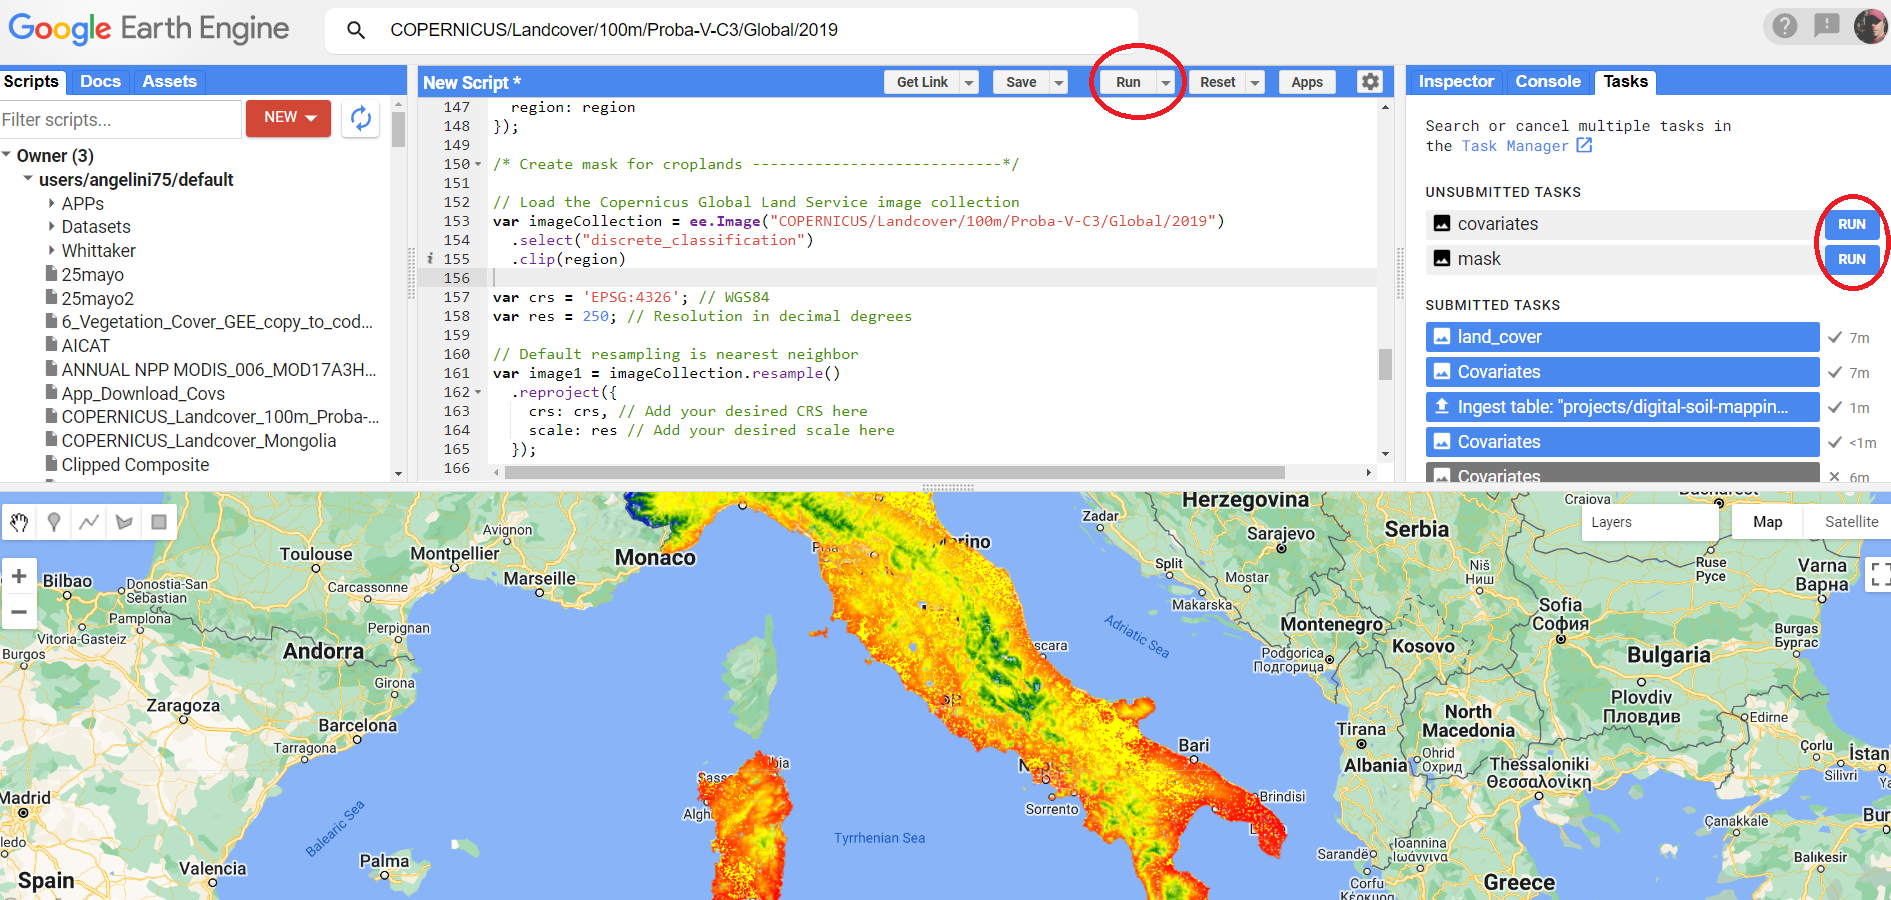
\includegraphics[width=1\linewidth]{images/GEE_export} \caption{Run button in code editor and RUN task in Tasks bar.}\label{fig:RUN}
\end{figure}

To run a task for exporting files to Google Drive in GEE, the Export.image.toDrive() function exports the image Google Drive. To start the task, you need to RUN the task, and it will be added to the GEE task list. You can monitor its progress and download the exported file once the task is complete.

\hypertarget{step-3-mapping-continuous-soil-properties}{%
\chapter{Step 3: Mapping continuous soil properties}\label{step-3-mapping-continuous-soil-properties}}

In this chapter, the cleaned soil data and the previously downloaded covariate layers are used to generate soil property maps using DSM techniques. These consist of merging soil and environmental covariates data, selecting the covariates, calibrating the machine learning model, assessing the uncertainty, predicting the soil properties and finally export the maps.

\hypertarget{mapping-soil-properties-with-random-forest}{%
\section{Mapping Soil Properties with Random Forest}\label{mapping-soil-properties-with-random-forest}}

Random Forest is a popular machine learning algorithm used in Digital Soil Mapping (DSM) for predicting the distribution of continuous soil properties. It leverages an ensemble of decision trees to improve the accuracy of predictions for the expected value of the target soil parameters.

In Random Forest, multiple individual decision trees are created, each trained on a random subset of the available data. These trees make independent predictions, and the final prediction is obtained by aggregating the predictions of all the trees. This ensemble approach helps to reduce the risk of overfitting and improves the model's generalization ability. Furthermore, Random Forest introduces an additional level of randomness by selecting different subsets of covariates (features) at each node of the trees. This feature sampling increases the independence between trees and helps mitigate potential collinearity issues in the individual regression tree models.

By combining the predictions of multiple trees and incorporating randomness in feature selection, Random Forest provides robust and reliable predictions for soil properties in DSM applications.

The main limitation of Random Forest is that it focuses primarily on predicting the mean value of the target variable thus it does not provide direct information about the variability or distribution of the target variable's predictions. This limits the possibility of assessment of the uncertainty of the predictions.

Quantile regression forests (QRF, Meinshausen (\protect\hyperlink{ref-Meinshausen2006}{2006})) are a generalisation of the random forest models, capable of not only predicting the conditional mean, but also the conditional probability density function. This provides a more comprehensive understanding of the full conditional distribution of the predictions, capturing the uncertainty and dispersion associated with different quantiles or levels of the target variable. This feature allows one to estimate the standard deviation of the prediction, as well as the likelihood of the target variable falling below a given threshold. By considering the dispersion of the predictions, QRF enables us to assess the model uncertainty and make more informed decisions. In a context where a minimum level of a soil nutrient concentration may be decisive for improving the crop yield, this feature can play an important role for the GSNmap initiative. Model calibration will be implemented using the caret package (\protect\hyperlink{ref-Kuhn2022}{Kuhn, 2022}). While we suggest to use QRF, caret provides a large set of models \url{https://topepo.github.io/caret/available-} models.html\#) that might perform better in specific cases. In this regard, it is up to the user to implement a different model, ensuring the product specifications.

We demonstrate the implementation of Quantile Regression Forest (QRF) for modeling and mapping soil properties and its associated uncertainty. The implementation presented here utilizes the Boruta, ranger, caret, and terra R packages.

\hypertarget{getting-prepared-to-map}{%
\section{Getting prepared to map}\label{getting-prepared-to-map}}

To begin, we open \emph{RStudio} and empty our global environment. Then, we set the working directory and assign the file path to our AOI shapefile to an R object. The target soil property that is going to be mapped in this exercise is Potassium denoted as `k' in the soil data table. Next, an R function that was built by the GSP is loaded from the training material folder. Finally, the packages that are going to be needed for mapping are called.

\begin{Shaded}
\begin{Highlighting}[]
\CommentTok{\#\_\_\_\_\_\_\_\_\_\_\_\_\_\_\_\_\_\_\_\_\_\_\_\_\_\_\_\_\_\_\_\_\_\_\_\_\_\_\_\_\_\_\_\_\_\_\_\_\_\_\_\_\_\_\_\_\_\_\_\_\_\_\_\_\_\_\_\_\_\_\_\_\_\_\_\_\_\_\_}
\CommentTok{\#}
\CommentTok{\# Quantile Regression Forest}
\CommentTok{\# Soil Property Mapping}
\CommentTok{\#}
\CommentTok{\# GSP{-}Secretariat}
\CommentTok{\# Contributors: Isabel Luotto (GSP{-}FAO)}
\CommentTok{\#               Marcos E. Angelini (GSP{-}FAO)}
\CommentTok{\#               Luis Rodríguez Lado (GSP{-}FAO)}
\CommentTok{\#               Stephen Roecker (NRCS{-}USDA)}
\CommentTok{\#\_\_\_\_\_\_\_\_\_\_\_\_\_\_\_\_\_\_\_\_\_\_\_\_\_\_\_\_\_\_\_\_\_\_\_\_\_\_\_\_\_\_\_\_\_\_\_\_\_\_\_\_\_\_\_\_\_\_\_\_\_\_\_\_\_\_\_\_\_\_\_\_\_\_\_\_\_\_\_}

\CommentTok{\#Empty environment and cache }
\FunctionTok{rm}\NormalTok{(}\AttributeTok{list =} \FunctionTok{ls}\NormalTok{())}
\FunctionTok{gc}\NormalTok{()}

\CommentTok{\# Content of this script =======================================================}
\CommentTok{\# 0 {-} Set working directory, soil attribute, and packages}
\CommentTok{\# 1 {-} Merge soil data with environmental covariates }
\CommentTok{\# 2 {-} Covariate selection}
\CommentTok{\# 3 {-} Model calibration}
\CommentTok{\# 4 {-} Uncertainty assessment}
\CommentTok{\# 5 {-} Prediction}
\CommentTok{\# 6 {-} Export final maps}
\CommentTok{\#\_\_\_\_\_\_\_\_\_\_\_\_\_\_\_\_\_\_\_\_\_\_\_\_\_\_\_\_\_\_\_\_\_\_\_\_\_\_\_\_\_\_\_\_\_\_\_\_\_\_\_\_\_\_\_\_\_\_\_\_\_\_\_\_\_\_\_\_\_\_\_\_\_\_\_\_\_\_\_}


\CommentTok{\# 0 {-} Set working directory, soil attribute, and packages ======================}

\CommentTok{\# Working directory}
\FunctionTok{setwd}\NormalTok{(}\FunctionTok{dirname}\NormalTok{(rstudioapi}\SpecialCharTok{::}\FunctionTok{getActiveDocumentContext}\NormalTok{()}\SpecialCharTok{$}\NormalTok{path))}
\FunctionTok{setwd}\NormalTok{(}\StringTok{".."}\NormalTok{)}

\CommentTok{\# Define country of interes throuhg 3{-}digit ISO code}
\NormalTok{ISO }\OtherTok{=}\StringTok{\textquotesingle{}ISO\textquotesingle{}}

\CommentTok{\# Load Area of interest (shp)}
\NormalTok{AOI }\OtherTok{\textless{}{-}} \StringTok{\textquotesingle{}01{-}Data/AOI.shp\textquotesingle{}}

\CommentTok{\# Terget soil attribute (Mandatory 10)}
\NormalTok{soilatt}\OtherTok{\textless{}{-}} \StringTok{"soc\_0\_30"} 

\CommentTok{\# Function for Uncertainty Assessment}
\FunctionTok{load}\NormalTok{(}\AttributeTok{file =} \StringTok{"03{-}Scripts/eval.RData"}\NormalTok{)}

\CommentTok{\#load packages}
\FunctionTok{library}\NormalTok{(tidyverse)}
\FunctionTok{library}\NormalTok{(caret)}
\FunctionTok{library}\NormalTok{(terra)}
\FunctionTok{library}\NormalTok{(Boruta)}
\FunctionTok{library}\NormalTok{(ranger)}
\end{Highlighting}
\end{Shaded}

Since soil data and environmental covariates are stored in different files and formats, it is necessary to first merge them into one dataframe. For this purpose, the covariate raster file is loaded into \textbf{R} from the covariates folder. Secondly, the table with the cleaned and quality checked soil data is loaded and converted to a shapefile using the lat/long coordinates columns.

\begin{Shaded}
\begin{Highlighting}[]
\CommentTok{\# 1 {-} Merge soil data with environmental covariates ============================}

\DocumentationTok{\#\# 1.1 {-} Load covariates {-}{-}{-}{-}{-}{-}{-}{-}{-}{-}{-}{-}{-}{-}{-}{-}{-}{-}{-}{-}{-}{-}{-}{-}{-}{-}{-}{-}{-}{-}{-}{-}{-}{-}{-}{-}{-}{-}{-}{-}{-}{-}{-}{-}{-}{-}{-}{-}{-}{-}{-}{-}{-}{-}{-}}
\NormalTok{covs }\OtherTok{\textless{}{-}} \FunctionTok{rast}\NormalTok{(}\StringTok{"01{-}Data/covs/Covariates.tif"}\NormalTok{) }\CommentTok{\# match case of the file name}
\NormalTok{ncovs }\OtherTok{\textless{}{-}} \FunctionTok{names}\NormalTok{(covs)}

\DocumentationTok{\#\# 1.2 {-} Load the soil data (Script 2) {-}{-}{-}{-}{-}{-}{-}{-}{-}{-}{-}{-}{-}{-}{-}{-}{-}{-}{-}{-}{-}{-}{-}{-}{-}{-}{-}{-}{-}{-}{-}{-}{-}{-}{-}{-}{-}{-}{-}{-}{-}}
\NormalTok{dat }\OtherTok{\textless{}{-}} \FunctionTok{read\_csv}\NormalTok{(}\StringTok{"02{-}Outputs/harmonized\_soil\_data.csv"}\NormalTok{)}

\CommentTok{\# Convert soil data into a spatial object (check https://epsg.io/6204)}
\NormalTok{dat }\OtherTok{\textless{}{-}} \FunctionTok{vect}\NormalTok{(dat, }\AttributeTok{geom=}\FunctionTok{c}\NormalTok{(}\StringTok{"x"}\NormalTok{, }\StringTok{"y"}\NormalTok{), }\AttributeTok{crs =} \FunctionTok{crs}\NormalTok{(covs))}
\end{Highlighting}
\end{Shaded}

The shapefile can be reprojected to match the CRS of the covariates using the project function of the terra package.

\begin{Shaded}
\begin{Highlighting}[]
\CommentTok{\# Reproject point coordinates to match coordinate system of covariates}
\NormalTok{dat }\OtherTok{\textless{}{-}}\NormalTok{ terra}\SpecialCharTok{::}\FunctionTok{project}\NormalTok{(dat, covs)}
\FunctionTok{names}\NormalTok{(dat) }
\end{Highlighting}
\end{Shaded}

Afterwards, the extract function can be used to sample the values of each covariate raster layer at the point location of each soil profile. This data is then merged in the dat dataframe. After checking the descriptive statistics of dat with the \texttt{summary()} command, the target soil attribute is selected together with the covariates. Finally, NA values (empty row values) are removed using the \texttt{na.omit()} function.

\begin{Shaded}
\begin{Highlighting}[]
\DocumentationTok{\#\# 1.3 {-} Extract values from covariates to the soil points {-}{-}{-}{-}{-}{-}{-}{-}{-}{-}{-}{-}{-}{-}{-}{-}{-}{-}{-}{-}{-}}
\NormalTok{pv }\OtherTok{\textless{}{-}}\NormalTok{ terra}\SpecialCharTok{::}\FunctionTok{extract}\NormalTok{(}\AttributeTok{x =}\NormalTok{ covs, }\AttributeTok{y =}\NormalTok{ dat, }\AttributeTok{xy=}\NormalTok{F)}
\NormalTok{dat }\OtherTok{\textless{}{-}} \FunctionTok{cbind}\NormalTok{(dat,pv)}
\NormalTok{dat }\OtherTok{\textless{}{-}} \FunctionTok{as.data.frame}\NormalTok{(dat)}

\FunctionTok{summary}\NormalTok{(dat)}
\end{Highlighting}
\end{Shaded}

\hypertarget{covariate-selection}{%
\section{Covariate selection}\label{covariate-selection}}

In a high-dimensional datasets, not all available features are equally informative for training a model. By detecting and subsetting the only relevant features for modeling, we can improve model's predictive performance, reduce its complexity, speeds up computations and enhance interpretability, allowing us to gain deeper insights into the underlying relationships within the data. Feature selection serves this purpose by identifying and retaining only those relevant features that are uncorrelated and non-redundant in the prediction of a target soil parameter, resulting in a more focused and effective model that is capable of making more accurate predictions.
Feature selection was implemented through the Boruta package (\protect\hyperlink{ref-miron2010}{Kursa and Rudnicki, 2010}), a feature selection algorithm that aims to identify the most relevant features in a dataset in both classification and regression problems. The algorithm is specifically designed for dealing with high-dimensional datasets and works by comparing the importance of each covariate against a randomized version of itself, known as shadow feature, that serve as a reference to determine whether the covariate has a higher importance than expected by chance.
The algorithm goes through a series of iterations, where it progressively eliminates irrelevant features. In each iteration, it evaluates the importance of each feature based on the random forest model and compares it to the importance of the corresponding shadow feature. If a feature's importance is significantly higher than its shadow, it is considered relevant and retained. Otherwise, it is deemed uninformative and removed. The iterations continue until all features are either confirmed as relevant or identified as uninformative. The final outcome is a set of relevant features (covariates) that are statistically significant in terms of their importance for explaining the target variable, thus reducing data dimensionality for improved model performance and interpretability.
The feature importance can be displayed in a graph showing different colors according to the importance of each feature in the model, with `green', `yellow', `red' and `blue' colors for `confirmed', `tentative', `rejected' and `shadow' features respectively (see \ref{fig:borutaplot}). Only those marked in green color are retained as valuable predictors.

\begin{Shaded}
\begin{Highlighting}[]
  \CommentTok{\# 2 {-} Covariate selection with Boruta package ==================================}
  \CommentTok{\# Wrapper feature selection algorithm}
  \DocumentationTok{\#\# 2.1 {-} Run the Boruta algorithm {-}{-}{-}{-}{-}{-}{-}{-}{-}{-}{-}{-}{-}{-}{-}{-}{-}{-}{-}{-}{-}{-}{-}{-}{-}{-}{-}{-}{-}{-}{-}{-}{-}{-}{-}{-}{-}{-}{-}{-}{-}{-}{-}{-}{-}{-}}
\NormalTok{  fs\_bor }\OtherTok{\textless{}{-}} \FunctionTok{Boruta}\NormalTok{(}\AttributeTok{y =}\NormalTok{ d[,soilatt], }\AttributeTok{x =}\NormalTok{ d[}\SpecialCharTok{{-}}\DecValTok{1}\NormalTok{], }\AttributeTok{maxRuns =} \DecValTok{100}\NormalTok{, }\AttributeTok{doTrace =} \DecValTok{1}\NormalTok{)}
  
  \DocumentationTok{\#\# 2.2 {-} Plot variable importance and selected features {-}{-}{-}{-}{-}{-}{-}{-}{-}{-}{-}{-}{-}{-}{-}{-}{-}{-}{-}{-}{-}{-}{-}{-}}
  \FunctionTok{png}\NormalTok{(}\AttributeTok{filename =} \FunctionTok{paste0}\NormalTok{(}\StringTok{"02{-}Outputs/importance\_"}\NormalTok{,soilatt,}\StringTok{".png"}\NormalTok{), }
       \AttributeTok{width =} \DecValTok{15}\NormalTok{, }\AttributeTok{height =} \DecValTok{25}\NormalTok{, }\AttributeTok{units =} \StringTok{"cm"}\NormalTok{, }\AttributeTok{res =} \DecValTok{600}\NormalTok{)}
  \FunctionTok{par}\NormalTok{(}\AttributeTok{las =} \DecValTok{2}\NormalTok{, }\AttributeTok{mar =} \FunctionTok{c}\NormalTok{(}\DecValTok{4}\NormalTok{, }\DecValTok{10}\NormalTok{, }\DecValTok{4}\NormalTok{, }\DecValTok{2}\NormalTok{) }\SpecialCharTok{+} \FloatTok{0.1}\NormalTok{)}
\NormalTok{  Boruta}\SpecialCharTok{:::}\FunctionTok{plot.Boruta}\NormalTok{(fs\_bor, }\AttributeTok{horizontal =} \ConstantTok{TRUE}\NormalTok{, }\AttributeTok{ylab =} \StringTok{""}\NormalTok{,}
                       \AttributeTok{xlab =} \StringTok{"Importance"}\NormalTok{, }\AttributeTok{cex.axis=}\FloatTok{0.60}\NormalTok{)}
  \FunctionTok{dev.off}\NormalTok{()}
  \DocumentationTok{\#\# 2.3 {-} Extract the selected feature variables {-}{-}{-}{-}{-}{-}{-}{-}{-}{-}{-}{-}{-}{-}{-}{-}{-}{-}{-}{-}{-}{-}{-}{-}{-}{-}{-}{-}{-}{-}{-}{-}}
\NormalTok{  (fs\_vars }\OtherTok{\textless{}{-}} \FunctionTok{getSelectedAttributes}\NormalTok{(fs\_bor, }\AttributeTok{withTentative =} \ConstantTok{TRUE}\NormalTok{))}
\end{Highlighting}
\end{Shaded}

The selected covariates can be visualised in Trellis displays. Finally, the optimal predictors are stored in a dedicated R object.

\begin{figure}
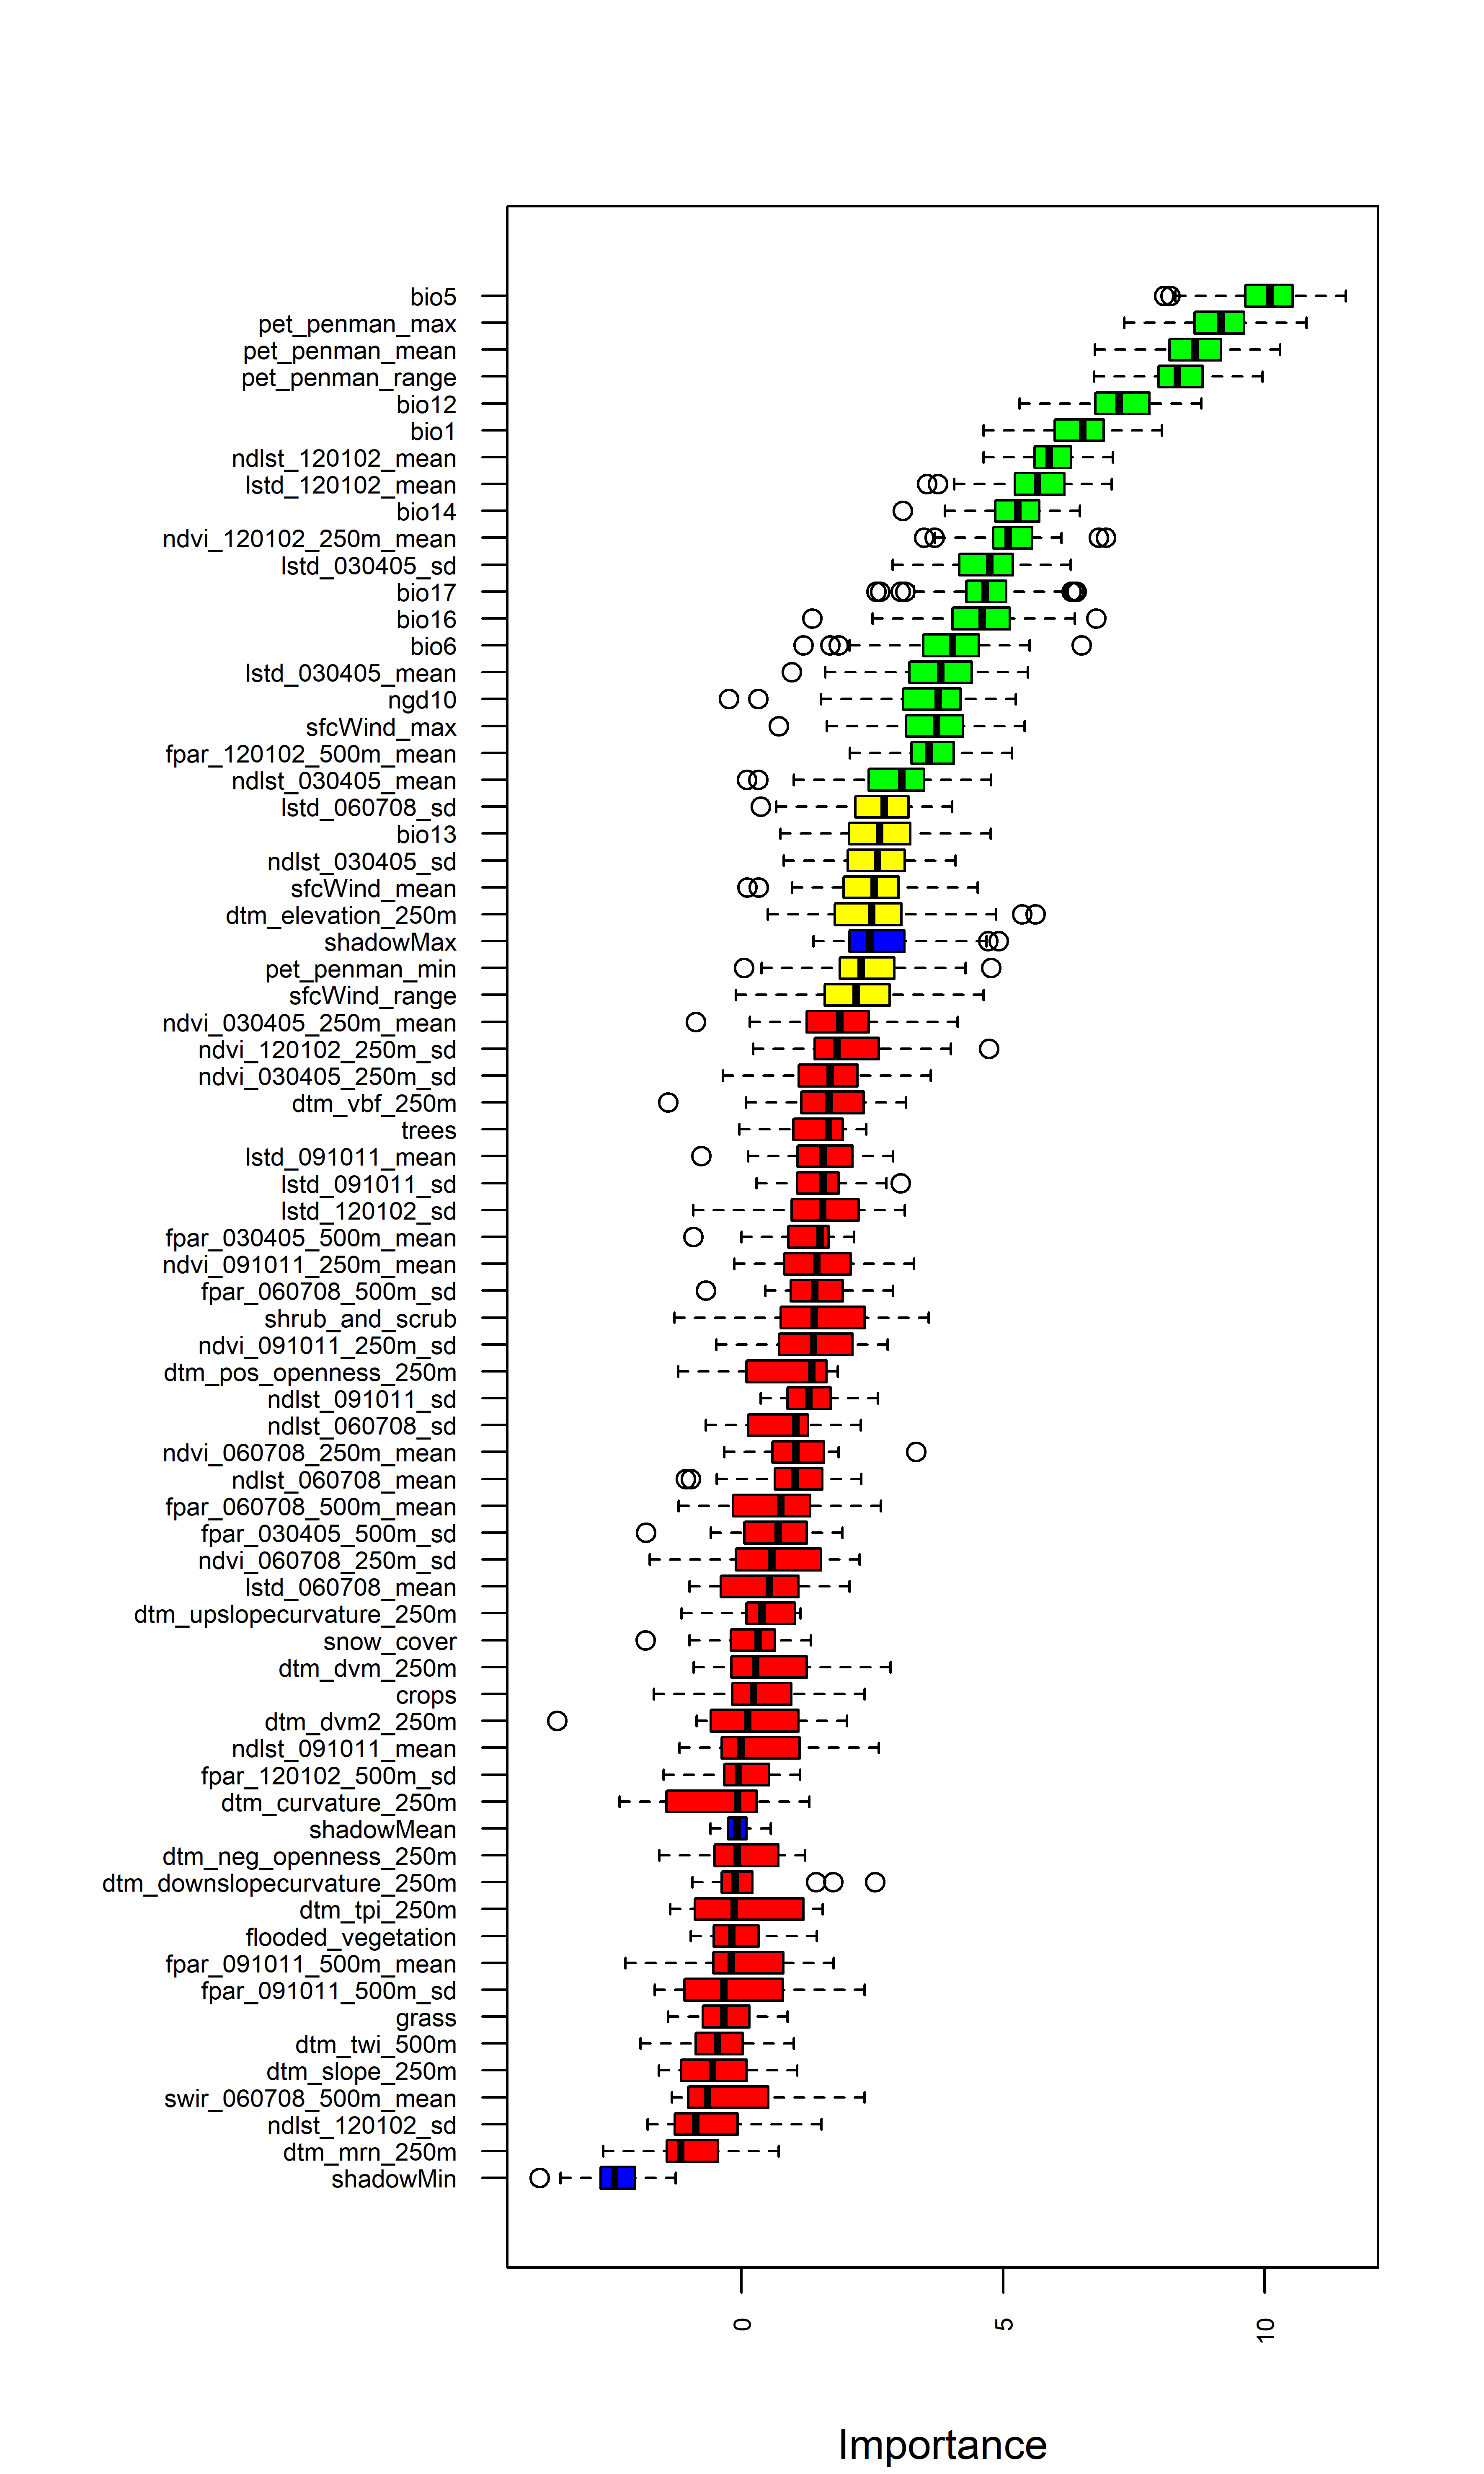
\includegraphics[width=1\linewidth]{images/importance_n_0_30} \caption{Covariates selecction for Total Nitrogen using Boruta algorithm.}\label{fig:borutaplot}
\end{figure}

\hypertarget{model-calibration}{%
\section{Model calibration}\label{model-calibration}}

The QRF model is calibrated using only the previous selection of covariates that actually have shown an effect on the target soil property. This is an important step to avoid overfitting of the model that can hamper a model's capacity to predict. Calibration is done by the `train' function from the caret package, utilizing the implementation of the random forest algorithm provided by the ranger package. During the model training, several important hyperparameters need to be set. These hyperparameters include:

\begin{itemize}
\item
  `mtry': This parameter determines the number of subset predictors considered for each split in the regression trees. It controls the level of randomness and feature diversity in the tree-building process.
\item
  `splitrule': This parameter specifies the criterion used to evaluate the quality of a potential split at each node of the tree. For regression problems, it is often set to ``variance,'' which measures the reduction in variance of the target variable achieved by splitting at a particular node. In our implementation, we consider three possible criteria: ``variance,'' ``extratrees,'' and ``maxstat.'' We select the criterion that produces the best calibrated model.
\item
  `min.node.size': This parameter represents the minimum number of observations (samples) required to create a terminal (leaf) node in a decision tree within the random forest algorithm. It ensures that each leaf contains a minimum number of observations to prevent overfitting and improve the generalization ability of the model. In regression problems, this number is typically set to 5.
\end{itemize}

Additionally, certain control parameters are necessary for training the model. These parameters are defined in the trainControl function and relate to the resampling method used to construct the bootstrap datasets. In our case, the resampling method is set to `repeatedcv,' with 10-fold cross-validation and 10 repetitions.

As cross-validation plays a crucial role in the model calibration step, we explain the process in detail at this stage. Cross-validation is a widely used method in Digital Soil Mapping (DSM) to assess the overall accuracy of the resulting maps. It involves randomly dividing the input data into a training set and a testing set. However, relying on a single testing dataset can introduce bias in the overall accuracy estimation. To mitigate this bias, we employ k-fold cross-validation. In this approach, the data is randomly partitioned into k parts, with one part used for testing and the remaining k-1 parts used for training the model. This process is repeated multiple times to enhance the robustness of parameter estimations. The final approach we adopt is known as repeated k-fold cross-validation, with k set to ten in this specific process. To help visualize the 10-fold cross-validation process, refer to Figure \ref{fig:cv}. Each row in the figure represents a step where the data is split into 10 subsets, with some samples marked as green balls representing the testing set, and others as yellow balls representing the training set. The figure illustrates how the data is divided into subsets in each step of the 10-fold process, and the blocks represent the repetition steps.
By employing repeated k-fold cross-validation, we can obtain a comprehensive assessment of the model's performance, ensuring reliable and robust parameter estimations for the final model.

\begin{figure}
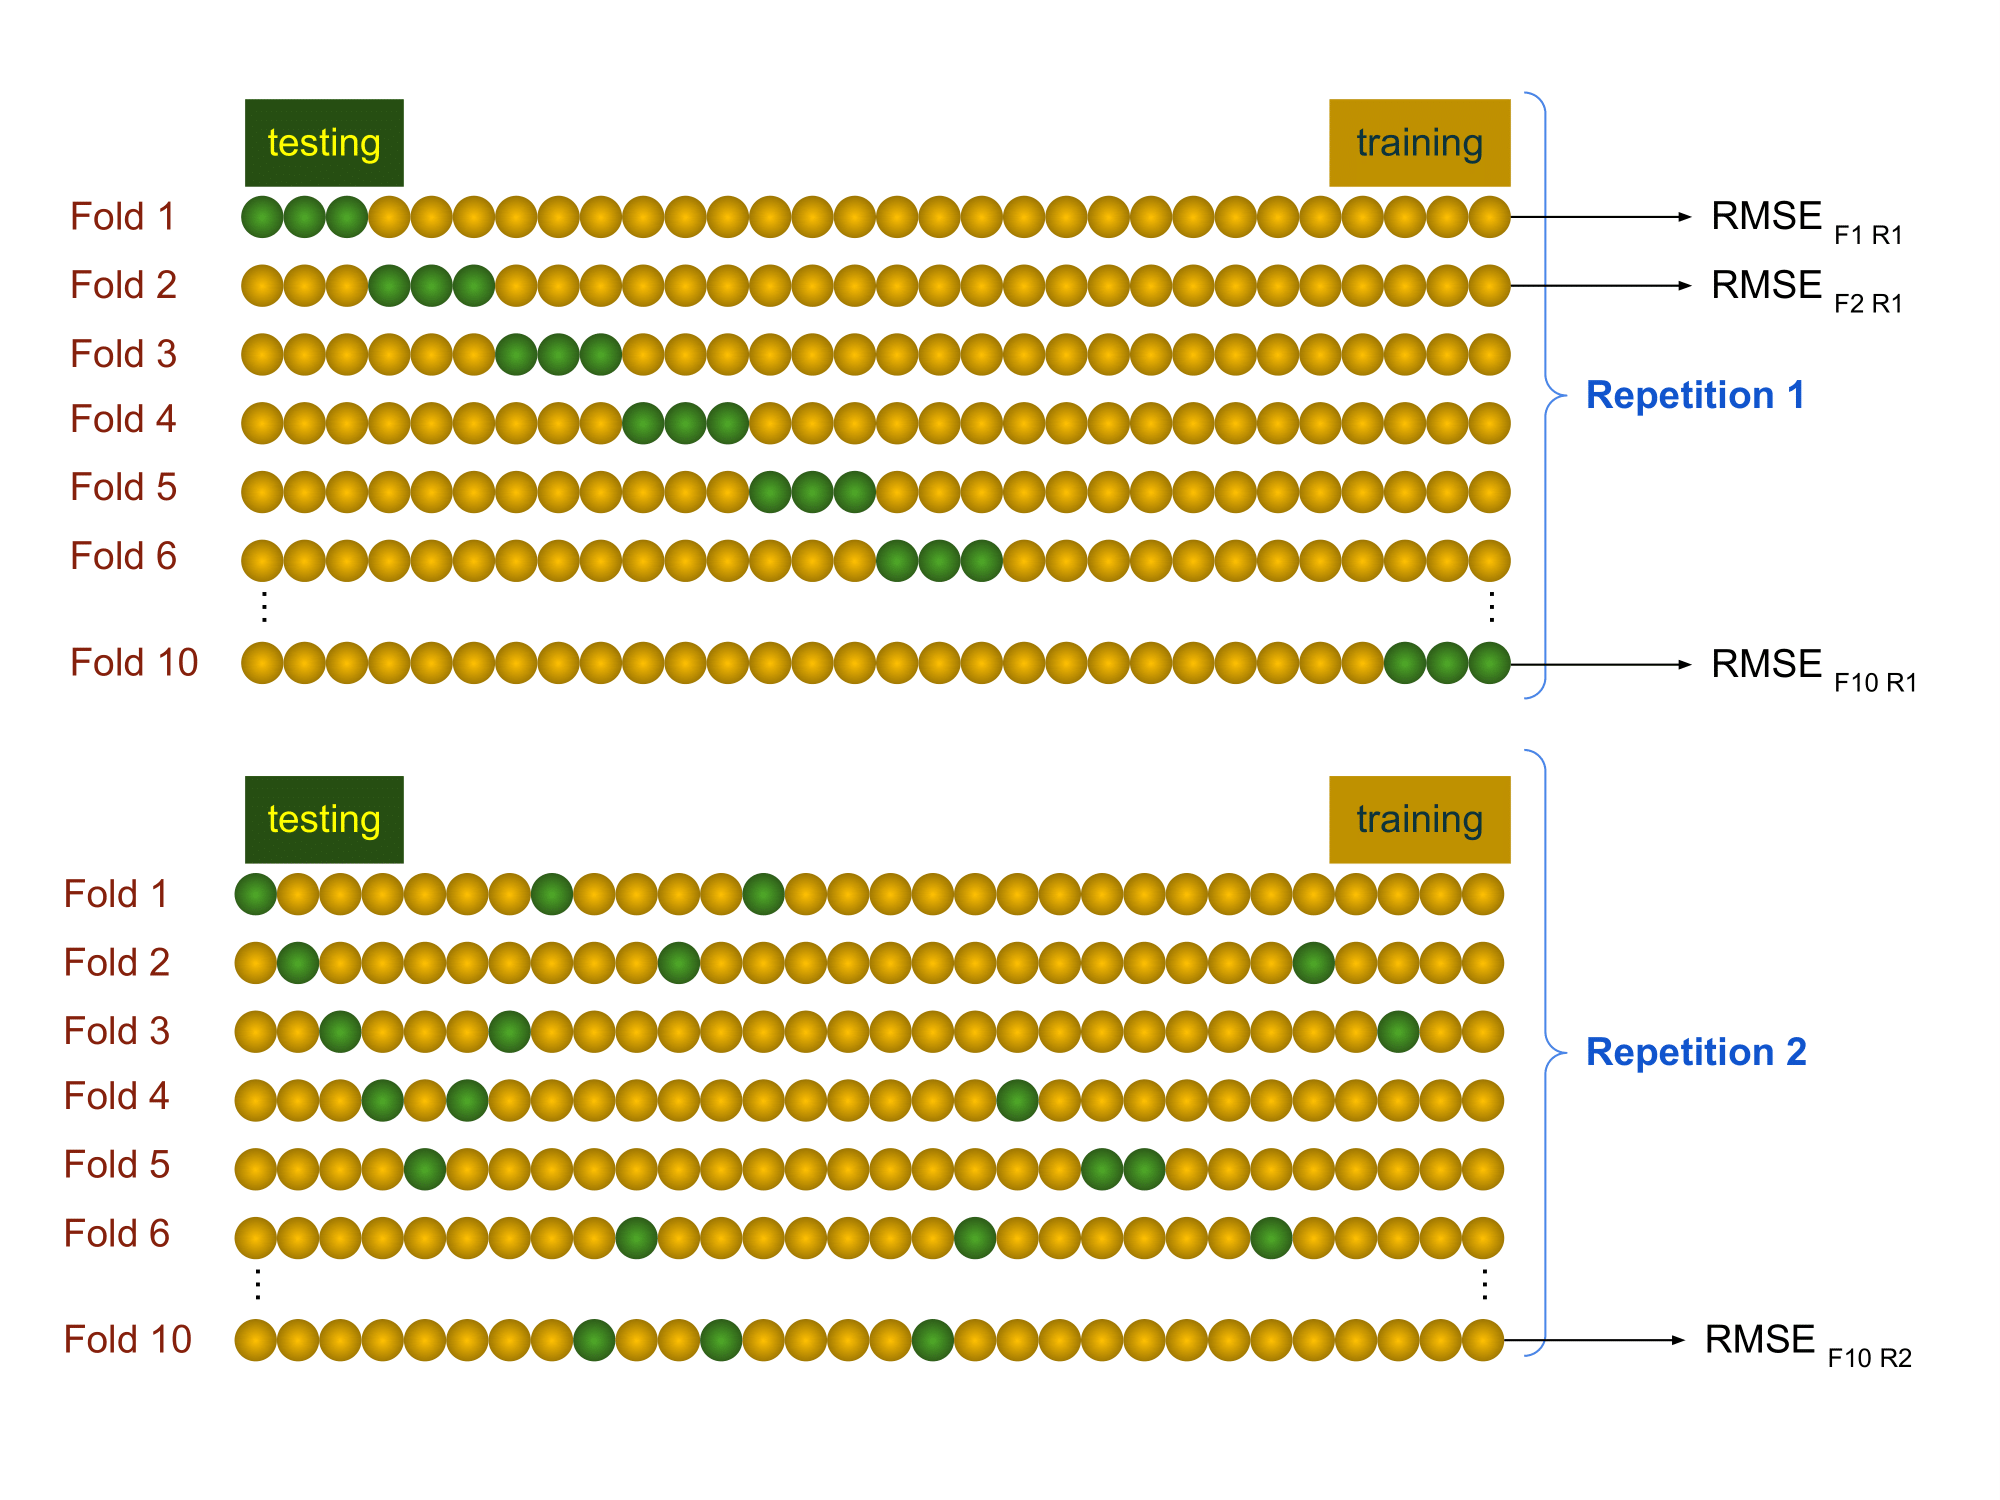
\includegraphics[width=1\linewidth]{images/cv} \caption{Schematic representation of the repeated cross-validation process.}\label{fig:cv}
\end{figure}

Repeated cross validation has been nicely implemented in the caret R package (\protect\hyperlink{ref-Kuhn2022}{Kuhn, 2022}), along with several calibration methods. Here, we use the \texttt{Boruta()} function to specify the modalities of the cross-validation that contain the abovementioned settings. These settings are stored in an object called ``fitControl''. Next, the user has to specify a formula that will be used in a regression. In line with the purpose of mapping the target soil property, the formula has Potassium as target variable (dependent variable) and all covariates as independent or explanatory variables.

\begin{Shaded}
\begin{Highlighting}[]
  \CommentTok{\# 3 {-} QRF Model calibration with ranger ========================================}
  \DocumentationTok{\#\# 3.1 {-} Set training parameters {-}{-}{-}{-}{-}{-}{-}{-}{-}{-}{-}{-}{-}{-}{-}{-}{-}{-}{-}{-}{-}{-}{-}{-}{-}{-}{-}{-}{-}{-}{-}{-}{-}{-}{-}{-}{-}{-}{-}{-}{-}{-}{-}{-}{-}{-}{-}}
\NormalTok{  fitControl }\OtherTok{\textless{}{-}} \FunctionTok{trainControl}\NormalTok{(}\AttributeTok{method =} \StringTok{"repeatedcv"}\NormalTok{,}
                             \AttributeTok{number =} \DecValTok{10}\NormalTok{,         }\DocumentationTok{\#\# 10 {-}fold CV}
                             \AttributeTok{repeats =} \DecValTok{10}\NormalTok{,        }\DocumentationTok{\#\# repeated 10 times}
                             \AttributeTok{savePredictions =} \ConstantTok{TRUE}\NormalTok{)}
  
  \DocumentationTok{\#\# 3.2 {-} Tune hyperparameters {-}{-}{-}{-}{-}{-}{-}{-}{-}{-}{-}{-}{-}{-}{-}{-}{-}{-}{-}{-}{-}{-}{-}{-}{-}{-}{-}{-}{-}{-}{-}{-}{-}{-}{-}{-}{-}{-}{-}{-}{-}{-}{-}{-}{-}{-}{-}{-}{-}{-}}
\NormalTok{  mtry }\OtherTok{\textless{}{-}} \FunctionTok{round}\NormalTok{(}\FunctionTok{length}\NormalTok{(fs\_vars)}\SpecialCharTok{/}\DecValTok{3}\NormalTok{)}
\NormalTok{  tuneGrid }\OtherTok{\textless{}{-}}  \FunctionTok{expand.grid}\NormalTok{(}
    \AttributeTok{mtry =} \FunctionTok{abs}\NormalTok{(}\FunctionTok{c}\NormalTok{(mtry}\SpecialCharTok{{-}}\FunctionTok{round}\NormalTok{(mtry}\SpecialCharTok{/}\DecValTok{2}\NormalTok{),}
\NormalTok{                 mtry}\SpecialCharTok{{-}}\FunctionTok{round}\NormalTok{(mtry}\SpecialCharTok{/}\DecValTok{3}\NormalTok{), }
\NormalTok{                 mtry, }
\NormalTok{                 mtry}\SpecialCharTok{+}\FunctionTok{round}\NormalTok{(mtry}\SpecialCharTok{/}\DecValTok{3}\NormalTok{),}
\NormalTok{                 mtry}\SpecialCharTok{+}\FunctionTok{round}\NormalTok{(mtry}\SpecialCharTok{/}\DecValTok{2}\NormalTok{))),}
    \AttributeTok{min.node.size =} \DecValTok{5}\NormalTok{,}
    \AttributeTok{splitrule =} \FunctionTok{c}\NormalTok{(}\StringTok{"variance"}\NormalTok{, }\StringTok{"extratrees"}\NormalTok{, }\StringTok{"maxstat"}\NormalTok{)}
\NormalTok{  )}
  
  \DocumentationTok{\#\# 3.3 {-} Calibrate the ranger model {-}{-}{-}{-}{-}{-}{-}{-}{-}{-}{-}{-}{-}{-}{-}{-}{-}{-}{-}{-}{-}{-}{-}{-}{-}{-}{-}{-}{-}{-}{-}{-}{-}{-}{-}{-}{-}{-}{-}{-}{-}{-}{-}{-}}
  \FunctionTok{print}\NormalTok{(soilatt)}
  \FunctionTok{print}\NormalTok{(}\StringTok{"training the model..."}\NormalTok{)}
\NormalTok{  model\_rn }\OtherTok{\textless{}{-}}\NormalTok{ caret}\SpecialCharTok{::}\FunctionTok{train}\NormalTok{(}
    \AttributeTok{y =}\NormalTok{ d[, soilatt], }\AttributeTok{x =}\NormalTok{ d[,fs\_vars],}
    \AttributeTok{method =} \StringTok{"ranger"}\NormalTok{,}
    \AttributeTok{quantreg =} \ConstantTok{TRUE}\NormalTok{,}
    \AttributeTok{importance =} \StringTok{"permutation"}\NormalTok{,}
    \AttributeTok{trControl =}\NormalTok{ fitControl,}
    \AttributeTok{verbose =} \ConstantTok{TRUE}\NormalTok{,}
    \AttributeTok{tuneGrid =}\NormalTok{ tuneGrid}
\NormalTok{  )}
  \FunctionTok{print}\NormalTok{(model\_rn)}
  \FunctionTok{print}\NormalTok{(model\_rn}\SpecialCharTok{$}\NormalTok{bestTune)}
\end{Highlighting}
\end{Shaded}

The results have been stored in an R object called model\_rn. To assess the contribution of each covariate on the model prediction. Finally, the model output is saved in the model folder within the Outputs folder - specifying the target soil properties.

\hypertarget{uncertainty-assessment}{%
\section{Uncertainty assessment}\label{uncertainty-assessment}}

Accuracy assessment is an essential step in digital soil mapping. One aspect of the accuracy assessment has been done in Step 7 by predicting the standard deviation of the prediction, which shows the spatial pattern of the uncertainty. Another aspect of the uncertainty is the estimation of the overall accuracy to measure the model performance. This will be measured using the model residuals generated by caret during the repeated cross validation step.
The residuals produced by caret consist of tabular data with observed and predicted values of the target soil property. They can be used to estimate different accuracy statistics. Wadoux, Walvoort and Brus (\protect\hyperlink{ref-Wadoux2022}{2022}) have reviewed and evaluated many of them. While they concluded that there is not a single accuracy statistic that can explain all aspect of map quality, they recommended the following:

The average error indices all relate to the difference between observed (z) and predicted (ẑ) value of soil property \emph{S} at the location \emph{i}. The error \(\epsilon\) is thus defined as:
\begin{equation}
\epsilon(S_{i}) = z(S_{i}) - \hat{z}(S_{i})
\end{equation}

The error indices that can be derived from this calculation inform about different aspects of prediction error and have the same unit as the target soil property. The mean prediction error (ME) estimates the prediction bias (see Eq. \eqref{eq:me}). If the ME is negative it means that the predicted values are below the observed ones. Conversely, a positive ME indicates a bias of the model towards higher predictions.

\begin{equation} 
  ME = \frac{1}{N}\sum_{i=1}^{N}\epsilon(S_{i})
  \label{eq:me}
\end{equation}

Mean absolute error (MAE) and root-mean squared error (RMSE) estimate the magnitude of errors. The MAE takes the absolute value of the ME thus quantifies the overall magnitude of the prediction error (see Eq.\eqref{eq:mae}). The closer the MAE is to 0 the more accurate is the model prediction.

\begin{equation} 
  MAE = \frac{1}{N}\sum_{i=1}^{N}|\epsilon(S_{i})|
  \label{eq:mae}
\end{equation}

Also, the RMSE provides a measure of the prediction error. Ideally, the RMSE approximates 0. Due to the squaring, larger absolute errors become more important (see Eq. \eqref{eq:rmse}). Thus, high absolute errors may lead to a worse RMSE measure. Therefore, it is best to calculate all three error indices to get a comprehensive picture.

\begin{equation} 
  RMSE = \sqrt{\frac{1}{N}\sum_{i=1}^{N}\epsilon(S_{i})^{2}}
  \label{eq:rmse}
\end{equation}

Besides the error indices, model quality can also be expressed by the coefficient of determination (R\textsuperscript{2}) which is the squared Pearson's product-moment correlation coefficient (r) (see Eq. \eqref{eq:r2}). The R\textsuperscript{2} takes values between 0 and 1. An R\textsuperscript{2} of 1 indicates total correlation between predicted and observed values whereas 0 indicates no correlation. The R\textsuperscript{2} can be biased by several factors and thus needs to be combined with other measures to yield a complete picture (\protect\hyperlink{ref-Wadoux2022}{Wadoux, Walvoort and Brus, 2022}).

\begin{equation} 
  r^2 = \frac{\sum_{i=1}^{N}(z(S_{i})-\overline{z})(\hat{z}(S_{i})-\overline{z})}{\sqrt{\sum_{i=1}^{N}(z(S_{i})-\overline{z})^2}\sqrt{\hat{z}(S_{i})-\overline{\hat{z}})^2}}
  \label{eq:r2}
\end{equation}

The Pearson's product-moment correlation coefficient (r) can take values between -1 and 1 and thus indicate the direction of the correlation (see Eq. \eqref{eq:r}).

\begin{equation} 
  r = \frac{\sum_{i=1}^{N}(z(S_{i})-\overline{z})(\hat{z}(S_{i})-\overline{z})}{\sqrt{\sum_{i=1}^{N}(z(S_{i})-\overline{z})^2}\sqrt{\hat{z}(S_{i})-\overline{\hat{z}})^2}}
  \label{eq:r}
\end{equation}

The modelling efficiency coefficient (MEC) accounts for the proportion of variance that is explained by a model (\protect\hyperlink{ref-Janssen1995}{Janssen and Heuberger, 1995}). It is calculated as the ratio of the RMSE and the variance (squared standard deviation) (see Eq. \eqref{eq:mec}). In a perfect scenario, the MEC equals 1. If the MEC equals 0, it means that the model does not predict the values better than the mean of the observed values would. In addition to that, the MEC can also take negative values if the RMSE is greater than the variance. In consequence, negative MECs indicate that the model predicts the values worse than the mean of the observed values.

\begin{equation} 
  MEC = 1 - \frac{\sum_{i=1}^{N}(z(S_{i})-\hat{z}(S_{i}))^2}{\sum_{i=1}^{N}(z(S_{i})-\overline{z})^2}
  \label{eq:mec}
\end{equation}

The R\^{}2, RMSE, and the MEC are susceptible to bias through large error values. Thus, caution needs to be taken when interpreting the indices presented here for accuracy assessment.

Now, back to the mapping exercise: In practical terms, before calculating any of these indices, it is necessary to first extract observed and predicted values and then store them in two separate R objects. Next, both values are combined to a dataframe.

\begin{Shaded}
\begin{Highlighting}[]
  \CommentTok{\# 4 {-} Accuracy assessment ======================================================}
  \DocumentationTok{\#\# 4.1 {-} extract observed and predicted values {-}{-}{-}{-}{-}{-}{-}{-}{-}{-}{-}{-}{-}{-}{-}{-}{-}{-}{-}{-}{-}{-}{-}{-}{-}{-}{-}{-}{-}{-}{-}{-}{-}}
\NormalTok{model\_rn }\OtherTok{\textless{}{-}} \FunctionTok{readRDS}\NormalTok{(}\StringTok{\textquotesingle{}Digital{-}Soil{-}Mapping/02{-}Outputs/models/ranger\_model\_soc\_0\_30.rds\textquotesingle{}}\NormalTok{)}

\NormalTok{  o }\OtherTok{\textless{}{-}}\NormalTok{ model\_rn}\SpecialCharTok{$}\NormalTok{pred }\SpecialCharTok{\%\textgreater{}\%} 
    \FunctionTok{filter}\NormalTok{(mtry }\SpecialCharTok{==}\NormalTok{ model\_rn}\SpecialCharTok{$}\NormalTok{bestTune}\SpecialCharTok{$}\NormalTok{mtry, }
\NormalTok{           splitrule}\SpecialCharTok{==}\NormalTok{model\_rn}\SpecialCharTok{$}\NormalTok{bestTune}\SpecialCharTok{$}\NormalTok{splitrule, }
\NormalTok{           min.node.size}\SpecialCharTok{==}\NormalTok{model\_rn}\SpecialCharTok{$}\NormalTok{bestTune}\SpecialCharTok{$}\NormalTok{min.node.size) }\SpecialCharTok{\%\textgreater{}\%} 
    \FunctionTok{select}\NormalTok{(obs) }\SpecialCharTok{\%\textgreater{}\%} \FunctionTok{as.vector}\NormalTok{() }\SpecialCharTok{\%\textgreater{}\%} \FunctionTok{unlist}\NormalTok{()}
\NormalTok{  p }\OtherTok{\textless{}{-}}\NormalTok{ model\_rn}\SpecialCharTok{$}\NormalTok{pred }\SpecialCharTok{\%\textgreater{}\%} 
    \FunctionTok{filter}\NormalTok{(mtry }\SpecialCharTok{==}\NormalTok{ model\_rn}\SpecialCharTok{$}\NormalTok{bestTune}\SpecialCharTok{$}\NormalTok{mtry, }
\NormalTok{           splitrule}\SpecialCharTok{==}\NormalTok{model\_rn}\SpecialCharTok{$}\NormalTok{bestTune}\SpecialCharTok{$}\NormalTok{splitrule, }
\NormalTok{           min.node.size}\SpecialCharTok{==}\NormalTok{model\_rn}\SpecialCharTok{$}\NormalTok{bestTune}\SpecialCharTok{$}\NormalTok{min.node.size) }\SpecialCharTok{\%\textgreater{}\%} 
    \FunctionTok{select}\NormalTok{(pred) }\SpecialCharTok{\%\textgreater{}\%} \FunctionTok{as.vector}\NormalTok{() }\SpecialCharTok{\%\textgreater{}\%} \FunctionTok{unlist}\NormalTok{()}
\NormalTok{  df }\OtherTok{\textless{}{-}} \FunctionTok{data.frame}\NormalTok{(o,p)}
\end{Highlighting}
\end{Shaded}

While solar diagrams (\protect\hyperlink{ref-Wadoux2022}{Wadoux, Walvoort and Brus, 2022}) are desired, we propose to produce a scatterplot of the observed vs predicted values maintaining the same range and scale for the X and Y axes. The dataframe is used for this purpose to plot observed values on the x-axis and predicted values on the y-axis.

\begin{Shaded}
\begin{Highlighting}[]
  \DocumentationTok{\#\# 4.2 {-} Plot and save scatterplot {-}{-}{-}{-}{-}{-}{-}{-}{-}{-}{-}{-}{-}{-}{-}{-}{-}{-}{-}{-}{-}{-}{-}{-}{-}{-}{-}{-}{-}{-}{-}{-}{-}{-}{-}{-}{-}{-}{-}{-}{-}{-}{-}{-}{-} }
\NormalTok{  (g1 }\OtherTok{\textless{}{-}} \FunctionTok{ggplot}\NormalTok{(df, }\FunctionTok{aes}\NormalTok{(}\AttributeTok{x =}\NormalTok{ o, }\AttributeTok{y =}\NormalTok{ p)) }\SpecialCharTok{+} 
     \FunctionTok{geom\_point}\NormalTok{(}\AttributeTok{alpha =} \FloatTok{0.3}\NormalTok{) }\SpecialCharTok{+} 
     \FunctionTok{geom\_abline}\NormalTok{(}\AttributeTok{slope =} \DecValTok{1}\NormalTok{, }\AttributeTok{intercept =} \DecValTok{0}\NormalTok{, }\AttributeTok{color =} \StringTok{"red"}\NormalTok{)}\SpecialCharTok{+}
     \FunctionTok{ylim}\NormalTok{(}\FunctionTok{c}\NormalTok{(}\FunctionTok{min}\NormalTok{(o), }\FunctionTok{max}\NormalTok{(o))) }\SpecialCharTok{+} \FunctionTok{theme}\NormalTok{(}\AttributeTok{aspect.ratio=}\DecValTok{1}\NormalTok{)}\SpecialCharTok{+} 
     \FunctionTok{labs}\NormalTok{(}\AttributeTok{title =}\NormalTok{ soilatt) }\SpecialCharTok{+} 
     \FunctionTok{xlab}\NormalTok{(}\StringTok{"Observed"}\NormalTok{) }\SpecialCharTok{+} \FunctionTok{ylab}\NormalTok{(}\StringTok{"Predicted"}\NormalTok{))}
\end{Highlighting}
\end{Shaded}

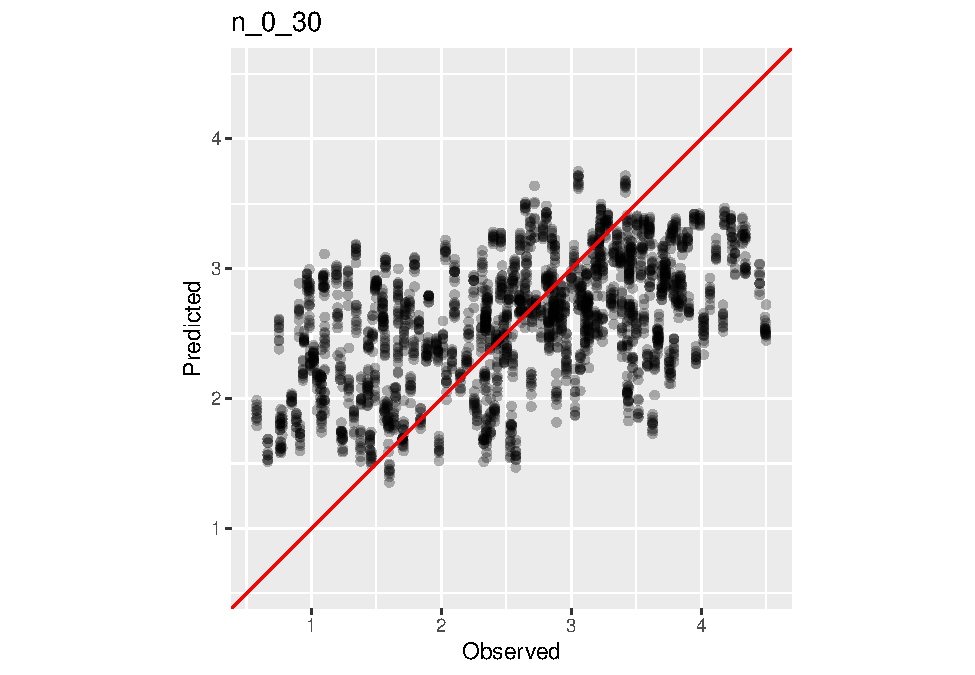
\includegraphics{GSNmap_Technical_Manual_files/figure-latex/unnamed-chunk-25-1.pdf}

\begin{Shaded}
\begin{Highlighting}[]
  \CommentTok{\# ggsave(g1, filename = paste0("02{-}Outputs/residuals\_",soilatt,".png"), scale = 1,}
  \CommentTok{\#        units = "cm", width = 12, height = 12)}
\end{Highlighting}
\end{Shaded}

Additionally, it is necessary to calculate standard metrics of error estimation. The function eval() below returns values for the ME, RMSE, MAE, the squared pearson correlation coefficient, the concordance correlation coefficient, scale shift and location shift relative to scale.

\begin{Shaded}
\begin{Highlighting}[]
\DocumentationTok{\#\# 4.2 {-} Print accuracy coeficients {-}{-}{-}{-}{-}{-}{-}{-}{-}{-}{-}{-}{-}{-}{-}{-}{-}{-}{-}{-}{-}{-}{-}{-}{-}{-}{-}{-}{-}{-}{-}{-}{-}{-}{-}{-}{-}{-}{-}{-}{-}{-}{-}{-}}
\CommentTok{\# https://github.com/AlexandreWadoux/MapQualityEvaluation}
\FunctionTok{print}\NormalTok{(}\FunctionTok{eval}\NormalTok{(df}\SpecialCharTok{$}\NormalTok{p,df}\SpecialCharTok{$}\NormalTok{o))}
\end{Highlighting}
\end{Shaded}

\begin{verbatim}
##     ME  MAE RMSE    r   r2  MEC rhoC  Cb
## 1 0.01 0.68 0.84 0.51 0.26 0.26  0.4 0.8
\end{verbatim}

\begin{table}

\caption{\label{tab:unnamed-chunk-28}Accuracy statistics.}
\centering
\begin{tabular}[t]{rrrrrrrr}
\toprule
ME & MAE & RMSE & r & r2 & MEC & rhoC & Cb\\
\midrule
8.87 & 275.69 & 372.82 & 0.7 & 0.5 & 0.5 & 0.66 & 0.94\\
\bottomrule
\end{tabular}
\end{table}

Finally, note that accuracy assessment has been discussed in Wadoux \emph{et al.} (\protect\hyperlink{ref-Wadoux2021}{2021}), since the spatial distribution of soil samples might constrain the validity of the accuracy statistics. This is especially true in cases where the spatial distribution of observations is clustered. The authors recommended creating a kriging map of residuals before using them for assessing the map quality.

\hypertarget{predicting-soil-attributes}{%
\section{Predicting soil attributes}\label{predicting-soil-attributes}}

After calibrating the model, caret will select the best set of parameters and will fit the model using the whole dataset. Then, the final model can be used to predict the target soil properties. The process uses the model and the values of the covariates at target locations. This is generally done by using the same input covariates as a multilayer raster format, ensuring that the names of the layers are the same as the covariates in the calibration dataset. In this step we will predict the conditional mean and conditional standard deviation at each raster cell.

To prevent for potential computational power limitations, first the raster is split into so-called tiles that divide the whole area of interest in multiple rasters with a coarse resolution. In this case 25 tiles are produced (5 rows x 5 columns). The functions for tiling come from the terra package. The predictions can also be hadled at one time by setting the parameters `nrows' and `ncols' in the `t' object to 1.

\begin{Shaded}
\begin{Highlighting}[]
  \CommentTok{\# 5 {-} Prediction ===============================================================}
  \CommentTok{\# Generation of maps (prediction of soil attributes) }
  \DocumentationTok{\#\# 5.1 {-} Produce tiles {-}{-}{-}{-}{-}{-}{-}{-}{-}{-}{-}{-}{-}{-}{-}{-}{-}{-}{-}{-}{-}{-}{-}{-}{-}{-}{-}{-}{-}{-}{-}{-}{-}{-}{-}{-}{-}{-}{-}{-}{-}{-}{-}{-}{-}{-}{-}{-}{-}{-}{-}{-}{-}{-}{-}{-}{-}}
  \CommentTok{\# r \textless{}{-}covs[[1]]}
  \CommentTok{\# t \textless{}{-} rast(nrows = 5, ncols = 5, extent = ext(r), crs = crs(r))}
  \CommentTok{\# tile \textless{}{-} makeTiles(r, t,overwrite=TRUE,filename="02{-}Outputs/tiles/tiles.tif")}
\end{Highlighting}
\end{Shaded}

Next, a for loop is formulated to predict each soil attribute for each tile. The tiling significantly improves the computational speed of the prediction. For each tile the mean and the standard deviation are stored in two separated objects that are then saved as raster files.

\begin{Shaded}
\begin{Highlighting}[]
  \DocumentationTok{\#\# 5.2 {-} Predict soil attributes per tiles {-}{-}{-}{-}{-}{-}{-}{-}{-}{-}{-}{-}{-}{-}{-}{-}{-}{-}{-}{-}{-}{-}{-}{-}{-}{-}{-}{-}{-}{-}{-}{-}{-}{-}{-}{-}{-}}
  \CommentTok{\# loop to predict soilatt on each tile}
  
    \ControlFlowTok{for}\NormalTok{ (j }\ControlFlowTok{in} \FunctionTok{seq\_along}\NormalTok{(tile)) \{}
    \FunctionTok{gc}\NormalTok{()}
    \CommentTok{\# read the tile}
\NormalTok{    t }\OtherTok{\textless{}{-}} \FunctionTok{rast}\NormalTok{(tile[j])}
    \CommentTok{\# crop the selected covariates with the tile j}
\NormalTok{    covst }\OtherTok{\textless{}{-}} \FunctionTok{crop}\NormalTok{(covs[[fs\_vars]], t)}
    
    \CommentTok{\# create a function to extract the predited values from ranger::predict.ranger()}
\NormalTok{    pfun }\OtherTok{\textless{}{-}}\NormalTok{ \textbackslash{}(...) \{ }\FunctionTok{predict}\NormalTok{(...)}\SpecialCharTok{$}\NormalTok{predictions }\SpecialCharTok{|\textgreater{}} \FunctionTok{t}\NormalTok{() \}}
    
    \CommentTok{\# predict conditional standard deviation}
\NormalTok{    terra}\SpecialCharTok{::}\FunctionTok{interpolate}\NormalTok{(covst, }
                       \AttributeTok{model =}\NormalTok{ model\_rn}\SpecialCharTok{$}\NormalTok{finalModel, }
                       \AttributeTok{fun=}\NormalTok{pfun, }
                       \AttributeTok{na.rm=}\ConstantTok{TRUE}\NormalTok{, }
                       \AttributeTok{type =} \StringTok{"quantiles"}\NormalTok{, }
                       \AttributeTok{what=}\NormalTok{sd,}
                       \AttributeTok{filename =} \FunctionTok{paste0}\NormalTok{(}\StringTok{"02{-}Outputs/tiles/soilatt\_tiles/"}\NormalTok{,}
\NormalTok{                                         soilatt,}\StringTok{"\_tileSD\_"}\NormalTok{, j, }\StringTok{".tif"}\NormalTok{), }
                       \AttributeTok{overwrite =} \ConstantTok{TRUE}\NormalTok{)}
    
    \CommentTok{\# predict conditional mean}
\NormalTok{    terra}\SpecialCharTok{::}\FunctionTok{interpolate}\NormalTok{(covst, }
                       \AttributeTok{model =}\NormalTok{ model\_rn}\SpecialCharTok{$}\NormalTok{finalModel, }
                       \AttributeTok{fun=}\NormalTok{pfun, }
                       \AttributeTok{na.rm=}\ConstantTok{TRUE}\NormalTok{, }
                       \AttributeTok{type =} \StringTok{"quantiles"}\NormalTok{, }
                       \AttributeTok{what=}\NormalTok{mean,}
                       \AttributeTok{filename =} \FunctionTok{paste0}\NormalTok{(}\StringTok{"02{-}Outputs/tiles/soilatt\_tiles/"}\NormalTok{,}
\NormalTok{                                         soilatt,}\StringTok{"\_tile\_"}\NormalTok{, j, }\StringTok{".tif"}\NormalTok{), }
                       \AttributeTok{overwrite =} \ConstantTok{TRUE}\NormalTok{)}
    
    \FunctionTok{print}\NormalTok{(}\FunctionTok{paste}\NormalTok{(}\StringTok{"tile"}\NormalTok{, j, }\StringTok{"of"}\NormalTok{, }\FunctionTok{length}\NormalTok{(tile)))}
\NormalTok{  \}}
\end{Highlighting}
\end{Shaded}

As a result, 25 tiles for the predicted mean and 25 tiles for the predicted standard deviation were produced using the QRF model. The next step is to merge these tiles to produce a map of the predicted mean and one of the predicted standard deviation. For this, again for loops are employed that read all raster file tiles. These are then put together by the mosaic() function of the terra package. Finally, they are masked to the AOI and then can be visualised in a figure.

\begin{Shaded}
\begin{Highlighting}[]
  \DocumentationTok{\#\# 5.3 {-} Merge tiles both prediction and st.Dev {-}{-}{-}{-}{-}{-}{-}{-}{-}{-}{-}{-}{-}{-}{-}{-}{-}{-}{-}{-}{-}{-}{-}{-}{-}{-}{-}{-}{-}{-}{-}{-}}
\NormalTok{  f\_mean }\OtherTok{\textless{}{-}} \FunctionTok{list.files}\NormalTok{(}\AttributeTok{path =} \StringTok{"02{-}Outputs/tiles/soilatt\_tiles/"}\NormalTok{, }
                       \AttributeTok{pattern =} \FunctionTok{paste0}\NormalTok{(soilatt,}\StringTok{"\_tile\_"}\NormalTok{), }\AttributeTok{full.names =} \ConstantTok{TRUE}\NormalTok{)}
\NormalTok{  f\_sd }\OtherTok{\textless{}{-}} \FunctionTok{list.files}\NormalTok{(}\AttributeTok{path =} \StringTok{"02{-}Outputs/tiles/soilatt\_tiles/"}\NormalTok{, }
                     \AttributeTok{pattern =}  \FunctionTok{paste0}\NormalTok{(soilatt,}\StringTok{"\_tileSD\_"}\NormalTok{), }\AttributeTok{full.names =} \ConstantTok{TRUE}\NormalTok{)}
\NormalTok{  r\_mean\_l }\OtherTok{\textless{}{-}} \FunctionTok{list}\NormalTok{()}
\NormalTok{  r\_sd\_l }\OtherTok{\textless{}{-}} \FunctionTok{list}\NormalTok{()}
  
  \ControlFlowTok{for}\NormalTok{ (g }\ControlFlowTok{in} \DecValTok{1}\SpecialCharTok{:}\FunctionTok{length}\NormalTok{(f\_mean))\{}
\NormalTok{    r }\OtherTok{\textless{}{-}} \FunctionTok{rast}\NormalTok{(f\_mean[g])}
\NormalTok{    r\_mean\_l[g] }\OtherTok{\textless{}{-}}\NormalTok{r}
    \FunctionTok{rm}\NormalTok{(r)}
\NormalTok{  \}}
  
  \ControlFlowTok{for}\NormalTok{ (g }\ControlFlowTok{in} \DecValTok{1}\SpecialCharTok{:}\FunctionTok{length}\NormalTok{(f\_sd))\{}
    
\NormalTok{    r }\OtherTok{\textless{}{-}} \FunctionTok{rast}\NormalTok{(f\_sd[g])}
\NormalTok{    r\_sd\_l[g] }\OtherTok{\textless{}{-}}\NormalTok{r}
    \FunctionTok{rm}\NormalTok{(r)}
\NormalTok{  \}}
\NormalTok{  r\_mean }\OtherTok{\textless{}{-}}\FunctionTok{sprc}\NormalTok{(r\_mean\_l)}
\NormalTok{  r\_sd }\OtherTok{\textless{}{-}}\FunctionTok{sprc}\NormalTok{(r\_sd\_l)}
  
\NormalTok{  pred\_mean }\OtherTok{\textless{}{-}} \FunctionTok{mosaic}\NormalTok{(r\_mean)}
\NormalTok{  pred\_sd }\OtherTok{\textless{}{-}} \FunctionTok{mosaic}\NormalTok{(r\_sd)}
  
\NormalTok{  aoi }\OtherTok{\textless{}{-}} \FunctionTok{vect}\NormalTok{(AOI)}
\NormalTok{  pred\_mean }\OtherTok{\textless{}{-}} \FunctionTok{mask}\NormalTok{(pred\_mean,aoi)}
\NormalTok{  pred\_sd }\OtherTok{\textless{}{-}} \FunctionTok{mask}\NormalTok{(pred\_sd,aoi)}
  
  
  \FunctionTok{plot}\NormalTok{(}\FunctionTok{c}\NormalTok{(pred\_mean, pred\_sd), }\AttributeTok{main =} \FunctionTok{paste}\NormalTok{(}\FunctionTok{c}\NormalTok{(}\StringTok{"mean"}\NormalTok{,}\StringTok{"sd"}\NormalTok{), soilatt), }
       \AttributeTok{col =} \FunctionTok{hcl.colors}\NormalTok{(}\DecValTok{100}\NormalTok{, }\StringTok{"Viridis"}\NormalTok{))}
\end{Highlighting}
\end{Shaded}

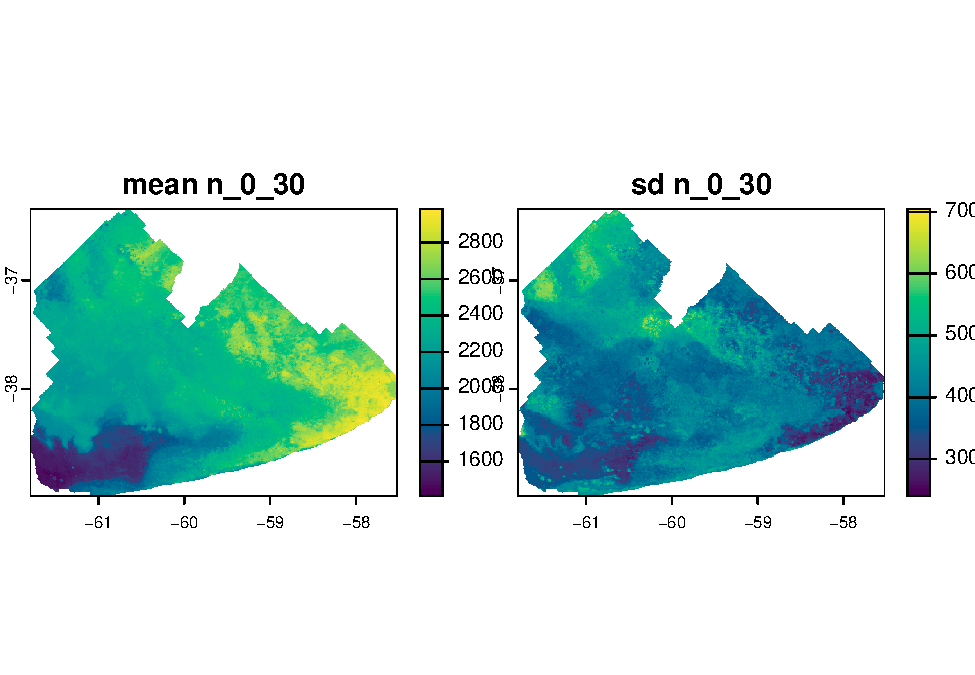
\includegraphics{GSNmap_Technical_Manual_files/figure-latex/unnamed-chunk-32-1.pdf}

The final step then consists of applying a cropland mask that is applied to the map and the uncertainty map since the soil data comes only from croplands and thus no assumption can be made to soil property values under different land covers. Additionally, a map is calculated to visualise the coefficient of variation (in Percent). The maps are then stored as raster files (GeoTiff/.tif) in the Outputs folder.

\begin{Shaded}
\begin{Highlighting}[]
  \CommentTok{\# 6 {-} Export final maps ========================================================}
  \DocumentationTok{\#\# 6.1 {-} Mask croplands {-}{-}{-}{-}{-}{-}{-}{-}{-}{-}{-}{-}{-}{-}{-}{-}{-}{-}{-}{-}{-}{-}{-}{-}{-}{-}{-}{-}{-}{-}{-}{-}{-}{-}{-}{-}{-}{-}{-}{-}{-}{-}{-}{-}{-}{-}{-}{-}{-}{-}{-}{-}{-}{-}{-}{-}}
\NormalTok{  msk }\OtherTok{\textless{}{-}} \FunctionTok{rast}\NormalTok{(}\StringTok{"01{-}Data/covs/mask.tif"}\NormalTok{)}
  \CommentTok{\# plot(msk)}
\NormalTok{  msk }\OtherTok{\textless{}{-}}\NormalTok{ terra}\SpecialCharTok{::}\FunctionTok{project}\NormalTok{(msk, pred\_mean)}
\NormalTok{  pred\_mean }\OtherTok{\textless{}{-}} \FunctionTok{mask}\NormalTok{(pred\_mean, msk)}
  \CommentTok{\# plot(pred\_mean)}
\NormalTok{  pred\_sd }\OtherTok{\textless{}{-}} \FunctionTok{mask}\NormalTok{(pred\_sd, msk)}
  \CommentTok{\# plot(pred\_sd)}
  \FunctionTok{plot}\NormalTok{(pred\_sd}\SpecialCharTok{/}\NormalTok{pred\_mean}\SpecialCharTok{*}\DecValTok{100}\NormalTok{, }\AttributeTok{main =} \FunctionTok{paste}\NormalTok{(}\StringTok{"Coeficient of variation"}\NormalTok{, soilatt), }
       \AttributeTok{col =} \FunctionTok{hcl.colors}\NormalTok{(}\DecValTok{100}\NormalTok{, }\StringTok{"Viridis"}\NormalTok{))}
  
  \DocumentationTok{\#\# 6.2 {-} Save results {-}{-}{-}{-}{-}{-}{-}{-}{-}{-}{-}{-}{-}{-}{-}{-}{-}{-}{-}{-}{-}{-}{-}{-}{-}{-}{-}{-}{-}{-}{-}{-}{-}{-}{-}{-}{-}{-}{-}{-}{-}{-}{-}{-}{-}{-}{-}{-}{-}{-}{-}{-}{-}{-}{-}{-}{-}{-}}
  \FunctionTok{writeRaster}\NormalTok{(pred\_mean, }
              \FunctionTok{paste0}\NormalTok{(}\StringTok{"02{-}Outputs/maps/"}\NormalTok{,ISO,}\StringTok{"\_GSNmap\_mean\_"}\NormalTok{,soilatt, }\StringTok{".tif"}\NormalTok{),}
              \AttributeTok{overwrite=}\ConstantTok{TRUE}\NormalTok{)}
  \FunctionTok{writeRaster}\NormalTok{(pred\_sd, }
              \FunctionTok{paste0}\NormalTok{(}\StringTok{"02{-}Outputs/maps/"}\NormalTok{,ISO,}\StringTok{"\_GSNmap\_sd\_"}\NormalTok{,soilatt, }\StringTok{".tif"}\NormalTok{),}
              \AttributeTok{overwrite=}\ConstantTok{TRUE}\NormalTok{)}
\end{Highlighting}
\end{Shaded}

\hypertarget{reporting-results}{%
\chapter{Reporting results}\label{reporting-results}}

The GSNmap consists of a set of mandatory and optional maps that are to be generated as raster files (GeoTiff) at a resolution of 250 x 250 m and at the mandatory depth of 0-30 cm.

The Mandatory data products are:

\begin{itemize}
\tightlist
\item
  total N
\item
  available P
\item
  available K
\item
  CEC
\item
  soil pH
\item
  clay, silt, and sand
\item
  soil organic carbon concentration
\item
  bulk density
\end{itemize}

Additionally, maps at deeper depths 30-60 cm and/or about micronutrients such as Ca, S, Mg, Fe, B, Cl, Mn, Zn, Cu, Mo, and Ni can be provided. All layers need to be submitted with the corresponding standard deviation layers.

An Rmarkdown script (with the extension .Rmd) is provided in the folder National Report. Script 5 can be used to translate the rmarkdown file into an automated report as a Word docx file.

\begin{Shaded}
\begin{Highlighting}[]
\CommentTok{\#\_\_\_\_\_\_\_\_\_\_\_\_\_\_\_\_\_\_\_\_\_\_\_\_\_\_\_\_\_\_\_\_\_\_\_\_\_\_\_\_\_\_\_\_\_\_\_\_\_\_\_\_\_\_\_\_\_\_\_\_\_\_\_\_\_\_\_\_\_\_\_\_\_\_\_\_\_\_\_}
\CommentTok{\#}
\CommentTok{\# QA/QC}
\CommentTok{\# Soil Property Mapping}
\CommentTok{\#}
\CommentTok{\# GSP{-}Secretariat}
\CommentTok{\# Contact: Isabel.Luotto@fao.org}
\CommentTok{\#          Marcos.Angelini@fao.org}
\CommentTok{\#\_\_\_\_\_\_\_\_\_\_\_\_\_\_\_\_\_\_\_\_\_\_\_\_\_\_\_\_\_\_\_\_\_\_\_\_\_\_\_\_\_\_\_\_\_\_\_\_\_\_\_\_\_\_\_\_\_\_\_\_\_\_\_\_\_\_\_\_\_\_\_\_\_\_\_\_\_\_\_}

\CommentTok{\#Empty environment and cache }
\FunctionTok{rm}\NormalTok{(}\AttributeTok{list =} \FunctionTok{ls}\NormalTok{())}
\FunctionTok{gc}\NormalTok{()}

\CommentTok{\# Content of this script =======================================================}
\CommentTok{\# 0 {-} Setup and user{-}defined variables}
\CommentTok{\# 1 {-}  User{-}defined variables}
\CommentTok{\# 2 {-} Render the .Rmd file to generate an automated report as a docx}
\CommentTok{\#\_\_\_\_\_\_\_\_\_\_\_\_\_\_\_\_\_\_\_\_\_\_\_\_\_\_\_\_\_\_\_\_\_\_\_\_\_\_\_\_\_\_\_\_\_\_\_\_\_\_\_\_\_\_\_\_\_\_\_\_\_\_\_\_\_\_\_\_\_\_\_\_\_\_\_\_\_\_\_}


\CommentTok{\# 0 {-} Initial Setup ============================================================}


\CommentTok{\#install.packages("rmarkdown")}
\CommentTok{\#tinytex::install\_tinytex()}
\CommentTok{\# library(sf)}
\CommentTok{\# library(ggplot2)}
\CommentTok{\# library(tidyverse)}
\CommentTok{\# library(terra)}
\FunctionTok{library}\NormalTok{(knitr)}
\CommentTok{\# library(tidyterra)}
\CommentTok{\# library(patchwork)}

\CommentTok{\# Working directory}
\FunctionTok{setwd}\NormalTok{(}\FunctionTok{dirname}\NormalTok{(rstudioapi}\SpecialCharTok{::}\FunctionTok{getActiveDocumentContext}\NormalTok{()}\SpecialCharTok{$}\NormalTok{path))}
\FunctionTok{setwd}\NormalTok{(}\StringTok{".."}\NormalTok{)}

\CommentTok{\# 1 {-}  User{-}defined variables ==================================================}

\CommentTok{\# Specify three{-}digit ISO code for your country}
\NormalTok{ISO }\OtherTok{\textless{}{-}} \StringTok{\textquotesingle{}AOI\textquotesingle{}}

\CommentTok{\# Specify the properties you mapped (the code assumes harmonized naming)}
\CommentTok{\# using the output data frame from script 2}
\NormalTok{dxy }\OtherTok{\textless{}{-}} \FunctionTok{read.csv}\NormalTok{(}\StringTok{"02{-}Outputs/harmonized\_soil\_data.csv"}\NormalTok{)}

\NormalTok{target\_properties }\OtherTok{\textless{}{-}} \FunctionTok{names}\NormalTok{(dxy)[ }\SpecialCharTok{!}\NormalTok{(}\FunctionTok{names}\NormalTok{(dxy)}\SpecialCharTok{\%in\%} \FunctionTok{c}\NormalTok{(}\StringTok{"ProfID"}\NormalTok{, }\StringTok{"x"}\NormalTok{ ,}\StringTok{"y"}\NormalTok{))]}

\CommentTok{\#target\_properties\textless{}{-}c(\textquotesingle{}ph\_0\_30\textquotesingle{})}

\CommentTok{\# Map background file}
\NormalTok{bckg}\OtherTok{\textless{}{-}}\FunctionTok{vect}\NormalTok{(}\StringTok{\textquotesingle{}01{-}Data/AOI.shp\textquotesingle{}}\NormalTok{)}

\CommentTok{\#Adjust figure width and height of the map plot}

\NormalTok{figw }\OtherTok{\textless{}{-}} \DecValTok{12}
\NormalTok{figh }\OtherTok{\textless{}{-}}\DecValTok{8}


\CommentTok{\# Specify where you want your word document to be saved}
\NormalTok{output\_file }\OtherTok{=} \FunctionTok{paste0}\NormalTok{(}\StringTok{"National Report/Report\_GSNmap\_"}\NormalTok{,ISO,}\StringTok{".docx"}\NormalTok{)}

\CommentTok{\# 2 {-} Render the .Rmd file to generate an automated report as a docx ===========}
\NormalTok{path }\OtherTok{=} \StringTok{\textquotesingle{}National Report/National GSNmap Report.Rmd\textquotesingle{}}
\NormalTok{output\_format }\OtherTok{=} \StringTok{\textquotesingle{}word\_document\textquotesingle{}}
\NormalTok{rmarkdown}\SpecialCharTok{::}\FunctionTok{render}\NormalTok{(path, output\_format, output\_file)}
\end{Highlighting}
\end{Shaded}

The output report document is to be submitted along with the layers using a submission form provided by the GSP Secretariat.

\hypertarget{way-forward}{%
\chapter{Way forward}\label{way-forward}}

This technical manual provided step-by-step guidance on how to generate nutrient maps by means of quantile regression forest models within a digital soil mapping framework. The array of maps produced belongs to the first implementation phase of the GSNmap initiative and provides urgently needed data on nutrient stocks and soil properties that govern nutrient availability. Policymakers will be able to use this data to derive conclusions on where to concentrate efforts to improve soil and land management to strengthen agrifood systems.
The second phase of the GSNmap will make use of the first phase data products to derive nutrient budget maps. Therefore, additional datasets will be used for calculating input and output terms of nutrient stocks. The methodology is currently under development by the GSNmap working group.

\hypertarget{frequent-asked-questions-and-troubleshooting-answers}{%
\section{Frequent asked questions and Troubleshooting answers}\label{frequent-asked-questions-and-troubleshooting-answers}}

To be developed soon\ldots{}

\hypertarget{issues-in-the-gsnmap-technical-manual}{%
\section{Issues in the GSNmap Technical Manual}\label{issues-in-the-gsnmap-technical-manual}}

Please, report any issue in the GSNmap Technical Manual in its issues GitHub page \url{https://github.com/FAO-GSP/GSNmap-TM/issues}.

\hypertarget{get-help}{%
\section{Get help}\label{get-help}}

\begin{itemize}
\tightlist
\item
  Check the issues GitHub page \url{https://github.com/FAO-GSP/GSNmap-TM/issues}
\item
  Issues with R packages: search for solutions in \url{https://stackoverflow.com/}
\item
  \texttt{caret} package \url{https://topepo.github.io/caret/}
\item
  \texttt{terra} package \url{https://rspatial.org/terra/pkg/1-introduction.html}
\item
  \texttt{tidyverse} package \url{https://r4ds.had.co.nz/}
\item
  \texttt{sf} package \url{https://r-spatial.github.io/sf/}
\end{itemize}

\hypertarget{annex-i-compendium-of-r-scripts}{%
\chapter*{Annex I: Compendium of R scripts}\label{annex-i-compendium-of-r-scripts}}
\addcontentsline{toc}{chapter}{Annex I: Compendium of R scripts}

This chapter contains the complete list of R scripts to run the process of mapping soil nutrient and associated soil properties.

\hypertarget{script-0-introduction-to-r}{%
\section*{Script 0: Introduction to R}\label{script-0-introduction-to-r}}
\addcontentsline{toc}{section}{Script 0: Introduction to R}

\begin{Shaded}
\begin{Highlighting}[]
\CommentTok{\# Introduction to R}

\CommentTok{\# 0. Playground ================================================================}

\CommentTok{\# learn important keyboard shortcuts}
\CommentTok{\# Ctrl + enter for running code}
\CommentTok{\# tab after writing the first three characters of the function name}
\CommentTok{\# F1 to access the help}

\CommentTok{\# explore the use of \textless{}{-}, $, [], ==, !=, c(), :, data.frame(), list(), as.factor()}

\NormalTok{a }\OtherTok{\textless{}{-}} \DecValTok{10}\SpecialCharTok{:}\DecValTok{15}
\NormalTok{a[}\DecValTok{2}\NormalTok{]}
\NormalTok{a[}\DecValTok{2}\SpecialCharTok{:}\DecValTok{3}\NormalTok{]}
\NormalTok{b }\OtherTok{\textless{}{-}} \FunctionTok{c}\NormalTok{(}\StringTok{"1"}\NormalTok{, }\StringTok{"a"}\NormalTok{, a )}
\FunctionTok{length}\NormalTok{(b)}
\NormalTok{df }\OtherTok{\textless{}{-}} \FunctionTok{data.frame}\NormalTok{(}\AttributeTok{column\_a =} \DecValTok{1}\SpecialCharTok{:}\DecValTok{8}\NormalTok{, }\AttributeTok{column\_b =}\NormalTok{ b)}

\NormalTok{df[,}\DecValTok{1}\NormalTok{]}
\NormalTok{df}\SpecialCharTok{$}\NormalTok{column\_b}
\FunctionTok{as.numeric}\NormalTok{(df}\SpecialCharTok{$}\NormalTok{column\_b)}
\FunctionTok{plot}\NormalTok{(df)}

\NormalTok{df[}\DecValTok{1}\SpecialCharTok{:}\DecValTok{3}\NormalTok{,]}
\NormalTok{df[,}\DecValTok{1}\NormalTok{]}

\FunctionTok{as.factor}\NormalTok{(b)}

\NormalTok{d }\OtherTok{\textless{}{-}} \FunctionTok{list}\NormalTok{(a, b, df)}
\NormalTok{d}
\FunctionTok{names}\NormalTok{(d)}
\FunctionTok{names}\NormalTok{(d) }\OtherTok{\textless{}{-}} \FunctionTok{c}\NormalTok{(}\StringTok{"numeric\_vector"}\NormalTok{, }\StringTok{"character\_vector"}\NormalTok{, }\StringTok{"dataframe"}\NormalTok{)}
\NormalTok{d}
\NormalTok{d[[}\DecValTok{1}\NormalTok{]]}
\NormalTok{d}\SpecialCharTok{$}\NormalTok{numeric\_vector}

\NormalTok{a }\SpecialCharTok{==}\NormalTok{ b}
\NormalTok{a }\SpecialCharTok{!=}\NormalTok{ b}

\CommentTok{\# 1. Set working directory ===================================================== }
\FunctionTok{setwd}\NormalTok{(}\StringTok{"C:/GIT/Digital{-}Soil{-}Mapping/"}\NormalTok{)}

\CommentTok{\# 2. Install and load packages =================================================}
\CommentTok{\# readxl, tidyverse, and data.table packages using the functions}
\FunctionTok{install.packages}\NormalTok{(}\StringTok{"tidyverse"}\NormalTok{)}
\FunctionTok{install.packages}\NormalTok{(}\StringTok{"readxl"}\NormalTok{)}
\FunctionTok{install.packages}\NormalTok{(}\StringTok{"data.table"}\NormalTok{)}
\FunctionTok{library}\NormalTok{(tidyverse)}
\FunctionTok{library}\NormalTok{(readxl)}
\FunctionTok{library}\NormalTok{(data.table)}

\CommentTok{\# 3. Import an spreadsheet =====================================================}
\DocumentationTok{\#\# 3.1 Read the MS Excel file {-}{-}{-}{-}{-}{-}{-}{-}{-}{-}{-}{-}{-}{-}{-}{-}{-}{-}{-}{-}{-}{-}{-}{-}{-}{-}{-}{-}{-}{-}{-}{-}{-}{-}{-}{-}{-}{-}{-}{-}{-}{-}{-}{-}{-}{-}{-}{-}{-}{-}}
\CommentTok{\#Read the soil\_data.xlsx file, spreadsheet 2, using read\_excel }
\FunctionTok{read\_excel}\NormalTok{(}\AttributeTok{path =} \StringTok{"01{-}Data/soil\_data.xlsx"}\NormalTok{, }\AttributeTok{sheet =} \DecValTok{2}\NormalTok{)}

\DocumentationTok{\#\# 3.2 Read the csv file with the native function {-}{-}{-}{-}{-}{-}{-}{-}{-}{-}{-}{-}{-}{-}{-}{-}{-}{-}{-}{-}{-}{-}{-}{-}{-}{-}{-}{-}{-}{-}}
\CommentTok{\# 01{-}Data/horizon.csv}
\FunctionTok{read.csv}\NormalTok{(}\StringTok{"01{-}Data/soil\_profile\_data.csv"}\NormalTok{)}

\DocumentationTok{\#\# 3.3 Read the csv file with the tidyverse function {-}{-}{-}{-}{-}{-}{-}{-}{-}{-}{-}{-}{-}{-}{-}{-}{-}{-}{-}{-}{-}{-}{-}{-}{-}{-}{-}}
\FunctionTok{read\_csv}\NormalTok{(}\StringTok{"01{-}Data/soil\_profile\_data.csv"}\NormalTok{)}

\DocumentationTok{\#\# 3.4 Read the csv file with the data.table function {-}{-}{-}{-}{-}{-}{-}{-}{-}{-}{-}{-}{-}{-}{-}{-}{-}{-}{-}{-}{-}{-}{-}{-}{-}{-}}
\FunctionTok{fread}\NormalTok{(}\StringTok{"01{-}Data/soil\_profile\_data.csv"}\NormalTok{)}

\DocumentationTok{\#\# 3.5 Assign the dataframe to an object called dat {-}{-}{-}{-}{-}{-}{-}{-}{-}{-}{-}{-}{-}{-}{-}{-}{-}{-}{-}{-}{-}{-}{-}{-}{-}{-}{-}{-}}
\NormalTok{dat }\OtherTok{\textless{}{-}} \FunctionTok{read\_csv}\NormalTok{(}\StringTok{"01{-}Data/soil\_profile\_data.csv"}\NormalTok{)}

\CommentTok{\# 4. Tidyverse functions =======================================================}
\DocumentationTok{\#\# 4.1 Select pid, hip, top, bottom, ph\_h2o, cec from dat {-}{-}{-}{-}{-}{-}{-}{-}{-}{-}{-}{-}{-}{-}{-}{-}{-}{-}{-}{-}{-}}
\NormalTok{dat\_1 }\OtherTok{\textless{}{-}}\NormalTok{ dat }\SpecialCharTok{\%\textgreater{}\%} 
  \FunctionTok{select}\NormalTok{(id\_prof, id\_hor, top, bottom, ph\_h2o, cec)}

\DocumentationTok{\#\# 4.2 Filter: pick observations by their values {-}{-}{-}{-}{-}{-}{-}{-}{-}{-}{-}{-}{-}{-}{-}{-}{-}{-}{-}{-}{-}{-}{-}{-}{-}{-}{-}{-}{-}{-}{-}}
\CommentTok{\# filter observations with cec \textgreater{} 50 cmolc/100g}

\NormalTok{dat\_2 }\OtherTok{\textless{}{-}}\NormalTok{ dat\_1 }\SpecialCharTok{\%\textgreater{}\%} 
  \FunctionTok{filter}\NormalTok{(cec }\SpecialCharTok{\textgreater{}} \DecValTok{30}\NormalTok{)}

\NormalTok{dat\_2}
\DocumentationTok{\#\# 4.3 Mutate: create a new variable {-}{-}{-}{-}{-}{-}{-}{-}{-}{-}{-}{-}{-}{-}{-}{-}{-}{-}{-}{-}{-}{-}{-}{-}{-}{-}{-}{-}{-}{-}{-}{-}{-}{-}{-}{-}{-}{-}{-}{-}{-}{-}{-}}
\CommentTok{\# thickness = top {-} bottom}

\NormalTok{dat\_3 }\OtherTok{\textless{}{-}}\NormalTok{ dat\_2 }\SpecialCharTok{\%\textgreater{}\%} 
  \FunctionTok{mutate}\NormalTok{(}\AttributeTok{thickness =}\NormalTok{ bottom }\SpecialCharTok{{-}}\NormalTok{ top)}

\DocumentationTok{\#\# 4.4 Group\_by and summarise {-}{-}{-}{-}{-}{-}{-}{-}{-}{-}{-}{-}{-}{-}{-}{-}{-}{-}{-}{-}{-}{-}{-}{-}{-}{-}{-}{-}{-}{-}{-}{-}{-}{-}{-}{-}{-}{-}{-}{-}{-}{-}{-}{-}{-}{-}{-}{-}{-}{-}}
\CommentTok{\# group by variable pid}
\CommentTok{\# summarise taking the mean of pH and cec}

\NormalTok{dat\_4 }\OtherTok{\textless{}{-}}\NormalTok{ dat\_3 }\SpecialCharTok{\%\textgreater{}\%} 
  \FunctionTok{group\_by}\NormalTok{(id\_prof) }\SpecialCharTok{\%\textgreater{}\%} 
  \FunctionTok{summarise}\NormalTok{(}\AttributeTok{mean\_ph =} \FunctionTok{mean}\NormalTok{(ph\_h2o),}
            \AttributeTok{mean\_cec =} \FunctionTok{mean}\NormalTok{(cec))}

\DocumentationTok{\#\# 4.5 Reshape the table using pivot\_longer {-}{-}{-}{-}{-}{-}{-}{-}{-}{-}{-}{-}{-}{-}{-}{-}{-}{-}{-}{-}{-}{-}{-}{-}{-}{-}{-}{-}{-}{-}{-}{-}{-}{-}{-}{-}}
\CommentTok{\# use dat\_3}
\CommentTok{\# put the names of the variables ph\_h2o, cec and thickness in the column }
\CommentTok{\# variable and keep the rest of the table. Save in dat\_5 }

\NormalTok{dat\_5 }\OtherTok{\textless{}{-}}\NormalTok{ dat\_3 }\SpecialCharTok{\%\textgreater{}\%} 
  \FunctionTok{pivot\_longer}\NormalTok{(ph\_h2o}\SpecialCharTok{:}\NormalTok{thickness, }\AttributeTok{names\_to =} \StringTok{"soil\_property"}\NormalTok{, }\AttributeTok{values\_to =} \StringTok{"value"}\NormalTok{)}

\DocumentationTok{\#\# 4.6 Join the table sites.csv with dat\_3 {-}{-}{-}{-}{-}{-}{-}{-}{-}{-}{-}{-}{-}{-}{-}{-}{-}{-}{-}{-}{-}{-}{-}{-}{-}{-}{-}{-}{-}{-}{-}{-}{-}{-}{-}{-}{-}}
\CommentTok{\# Load soil\_phys\_data030.csv (in 01{-}Data folder) }
\CommentTok{\# Join its columns with dat\_3 keeping all the rows of dat\_3}
\CommentTok{\# save the result as dat\_6}

\NormalTok{phys }\OtherTok{\textless{}{-}} \FunctionTok{read\_csv}\NormalTok{(}\StringTok{"01{-}Data/soil\_phys\_data030.csv"}\NormalTok{)}

\NormalTok{phys }\OtherTok{\textless{}{-}}\NormalTok{ phys }\SpecialCharTok{\%\textgreater{}\%} \FunctionTok{rename}\NormalTok{(}\AttributeTok{id\_prof =} \StringTok{"ProfID"}\NormalTok{)}

\NormalTok{dat\_6 }\OtherTok{\textless{}{-}}\NormalTok{ dat\_3 }\SpecialCharTok{\%\textgreater{}\%} 
  \FunctionTok{left\_join}\NormalTok{(phys)}
\CommentTok{\# or}
\NormalTok{dat\_6 }\OtherTok{\textless{}{-}}\NormalTok{ phys }\SpecialCharTok{\%\textgreater{}\%} 
  \FunctionTok{right\_join}\NormalTok{(dat\_3)}

\CommentTok{\# 5. Data visualization with ggplot2 ===========================================}
\DocumentationTok{\#\# 5.1 1D plot: histograms {-}{-}{-}{-}{-}{-}{-}{-}{-}{-}{-}{-}{-}{-}{-}{-}{-}{-}{-}{-}{-}{-}{-}{-}{-}{-}{-}{-}{-}{-}{-}{-}{-}{-}{-}{-}{-}{-}{-}{-}{-}{-}{-}{-}{-}{-}{-}{-}{-}{-}{-}{-}{-}}
\CommentTok{\# histograms of cec and ph\_h2o}

\FunctionTok{ggplot}\NormalTok{(dat\_3, }\FunctionTok{aes}\NormalTok{(}\AttributeTok{x=}\NormalTok{cec)) }\SpecialCharTok{+} \FunctionTok{geom\_histogram}\NormalTok{()}

\DocumentationTok{\#\# 5.2 2D plot: scatterplot {-}{-}{-}{-}{-}{-}{-}{-}{-}{-}{-}{-}{-}{-}{-}{-}{-}{-}{-}{-}{-}{-}{-}{-}{-}{-}{-}{-}{-}{-}{-}{-}{-}{-}{-}{-}{-}{-}{-}{-}{-}{-}{-}{-}{-}{-}{-}{-}{-}{-}{-}{-}}
\CommentTok{\# Scatterplot bottom vs. ph\_h2o}

\FunctionTok{ggplot}\NormalTok{(dat\_3, }\FunctionTok{aes}\NormalTok{(}\AttributeTok{x =}\NormalTok{ bottom, }\AttributeTok{y =}\NormalTok{ ph\_h2o)) }\SpecialCharTok{+} 
  \FunctionTok{geom\_point}\NormalTok{() }

\CommentTok{\# add a fitting line}

\FunctionTok{ggplot}\NormalTok{(dat\_3, }\FunctionTok{aes}\NormalTok{(}\AttributeTok{x =}\NormalTok{ bottom, }\AttributeTok{y =}\NormalTok{ ph\_h2o)) }\SpecialCharTok{+} 
  \FunctionTok{geom\_point}\NormalTok{() }\SpecialCharTok{+}
  \FunctionTok{geom\_smooth}\NormalTok{(}\AttributeTok{method =} \StringTok{"lm"}\NormalTok{ )}

\DocumentationTok{\#\# 5.3 3D plot: scatterplot {-}{-}{-}{-}{-}{-}{-}{-}{-}{-}{-}{-}{-}{-}{-}{-}{-}{-}{-}{-}{-}{-}{-}{-}{-}{-}{-}{-}{-}{-}{-}{-}{-}{-}{-}{-}{-}{-}{-}{-}{-}{-}{-}{-}{-}{-}{-}{-}{-}{-}{-}{-}}
\CommentTok{\# Scatterplot bottom vs. ph\_h2o, add clay as color and size inside the }
\CommentTok{\# function aes()}

\FunctionTok{ggplot}\NormalTok{(dat\_3, }\FunctionTok{aes}\NormalTok{(}\AttributeTok{x =}\NormalTok{ bottom, }\AttributeTok{y =}\NormalTok{ ph\_h2o, }\AttributeTok{color =}\NormalTok{ cec, }\AttributeTok{size =}\NormalTok{ cec)) }\SpecialCharTok{+} 
  \FunctionTok{geom\_point}\NormalTok{()}

\CommentTok{\# 6. Geospatial data with terra ================================================}
\DocumentationTok{\#\# Load packages (install them if needed)}
\FunctionTok{library}\NormalTok{(terra)}
\DocumentationTok{\#\# 6.1 Load a raster and a vector layer {-}{-}{-}{-}{-}{-}{-}{-}{-}{-}{-}{-}{-}{-}{-}{-}{-}{-}{-}{-}{-}{-}{-}{-}{-}{-}{-}{-}{-}{-}{-}{-}{-}{-}{-}{-}{-}{-}{-}{-}}
\CommentTok{\# Load 01{-}Data/covs/grass.tif using rast() function, then plot it}
\CommentTok{\# Load 01{-}Data/soil map/SoilTypes.shp using vect() function and plot it }
\CommentTok{\# explore the attributes of these layers}

\NormalTok{r }\OtherTok{\textless{}{-}} \FunctionTok{rast}\NormalTok{(}\StringTok{"01{-}Data/Macedonia/grass.tif"}\NormalTok{)}
\FunctionTok{plot}\NormalTok{(r)}

\NormalTok{v }\OtherTok{\textless{}{-}} \FunctionTok{vect}\NormalTok{(}\StringTok{"01{-}Data/Macedonia/SoilTypes.shp"}\NormalTok{)}
\FunctionTok{plot}\NormalTok{(v)}

\DocumentationTok{\#\# 6.2 Load a raster and a vector layer {-}{-}{-}{-}{-}{-}{-}{-}{-}{-}{-}{-}{-}{-}{-}{-}{-}{-}{-}{-}{-}{-}{-}{-}{-}{-}{-}{-}{-}{-}{-}{-}{-}{-}{-}{-}{-}{-}{-}{-}}
\CommentTok{\# Check the current CRS (EPSG) of the raster and the vector. }
\CommentTok{\# Find a *projected* CRS in http://epsg.io for Macedonia and copy the number}
\CommentTok{\# Check the Arguments of function project (?project) that need to be defined}
\CommentTok{\# Save the new object as r\_proj and v\_proj}
\CommentTok{\# plot both objects}

\NormalTok{r\_proj }\OtherTok{\textless{}{-}} \FunctionTok{project}\NormalTok{(}\AttributeTok{x =}\NormalTok{ r, }\AttributeTok{y =} \StringTok{"epsg:6204"}\NormalTok{, }\AttributeTok{method =} \StringTok{"bilinear"}\NormalTok{, }\AttributeTok{res =} \DecValTok{250}\NormalTok{)}
\FunctionTok{plot}\NormalTok{(r\_proj)}
\NormalTok{v\_proj }\OtherTok{\textless{}{-}} \FunctionTok{project}\NormalTok{(}\AttributeTok{x =}\NormalTok{ v, }\AttributeTok{y =} \StringTok{"epsg:6204"}\NormalTok{)}
\FunctionTok{plot}\NormalTok{(v\_proj, }\AttributeTok{add =} \ConstantTok{TRUE}\NormalTok{)}

\DocumentationTok{\#\# 6.3 Cropping and masking a raster {-}{-}{-}{-}{-}{-}{-}{-}{-}{-}{-}{-}{-}{-}{-}{-}{-}{-}{-}{-}{-}{-}{-}{-}{-}{-}{-}{-}{-}{-}{-}{-}{-}{-}{-}{-}{-}{-}{-}{-}{-}{-}{-}}
\CommentTok{\# Compute the area of the polygons in v\_proj (search for a function) and}
\CommentTok{\# assign the values to a new column named area}
\CommentTok{\# select the largest polygon using [], $, == and max() func. and save it as pol}
\CommentTok{\# crop the raster with pol using the crop() function and save it as r\_pol}
\CommentTok{\# mask the raster r\_pol with the polygon pol and save it with the same name}
\CommentTok{\# plot each result}

\NormalTok{v\_proj}\SpecialCharTok{$}\NormalTok{area }\OtherTok{\textless{}{-}} \FunctionTok{expanse}\NormalTok{(v\_proj, }\AttributeTok{unit =} \StringTok{"ha"}\NormalTok{)}
\NormalTok{pol }\OtherTok{\textless{}{-}}\NormalTok{ v\_proj[v\_proj}\SpecialCharTok{$}\NormalTok{area }\SpecialCharTok{==} \FunctionTok{max}\NormalTok{(v\_proj}\SpecialCharTok{$}\NormalTok{area)]}
\FunctionTok{plot}\NormalTok{(pol)}
\NormalTok{r\_pol }\OtherTok{\textless{}{-}} \FunctionTok{crop}\NormalTok{(r\_proj, pol)}
\FunctionTok{plot}\NormalTok{(r\_pol)}
\FunctionTok{plot}\NormalTok{(pol, }\AttributeTok{add =} \ConstantTok{TRUE}\NormalTok{)}
\NormalTok{r\_pol }\OtherTok{\textless{}{-}} \FunctionTok{mask}\NormalTok{(r\_pol, pol)}
\FunctionTok{plot}\NormalTok{(r\_pol)}

\DocumentationTok{\#\# 6.4 Replace values in a raster by filtering their cells {-}{-}{-}{-}{-}{-}{-}{-}{-}{-}{-}{-}{-}{-}{-}{-}{-}{-}{-}{-}{-}}
\CommentTok{\# Explore the following link to understand how terra manage cell values}
\CommentTok{\# https://rspatial.org/terra/pkg/4{-}algebra.html }
\CommentTok{\# Replace values lower than 5 in r+pol by 0}

\NormalTok{r\_pol[r\_pol}\SpecialCharTok{$}\NormalTok{grass }\SpecialCharTok{\textless{}} \DecValTok{5}\NormalTok{] }\OtherTok{\textless{}{-}} \DecValTok{0}
\FunctionTok{plot}\NormalTok{(r\_pol)}

\DocumentationTok{\#\# 6.5 Rasterize a vector layer {-}{-}{-}{-}{-}{-}{-}{-}{-}{-}{-}{-}{-}{-}{-}{-}{-}{-}{-}{-}{-}{-}{-}{-}{-}{-}{-}{-}{-}{-}{-}{-}{-}{-}{-}{-}{-}{-}{-}{-}{-}{-}{-}{-}{-}{-}{-}{-}}
\CommentTok{\# Use rasterize() function to convert v\_proj to raster}
\CommentTok{\# Use r\_proj as reference raster}
\CommentTok{\# Use field Symbol to assign cell values, and plot the new map}

\NormalTok{v\_class }\OtherTok{\textless{}{-}} \FunctionTok{rasterize}\NormalTok{(}\AttributeTok{x =}\NormalTok{ v\_proj, }\AttributeTok{y =}\NormalTok{ r\_proj, }\AttributeTok{field =} \StringTok{"Symbol"}\NormalTok{ )}
\FunctionTok{plot}\NormalTok{(v\_class)}
\NormalTok{v\_class}
\FunctionTok{activeCat}\NormalTok{(v\_class) }\OtherTok{\textless{}{-}} \DecValTok{1}

\DocumentationTok{\#\# 6.6 Extracting raster values using points {-}{-}{-}{-}{-}{-}{-}{-}{-}{-}{-}{-}{-}{-}{-}{-}{-}{-}{-}{-}{-}{-}{-}{-}{-}{-}{-}{-}{-}{-}{-}{-}{-}{-}{-}}
\CommentTok{\# Covert dat\_6 to spatial points using vect() function (check help of vect())}
\CommentTok{\# Note that the EPSG number is 6204}
\CommentTok{\# Save the points as s}
\CommentTok{\# Plot s and r\_proj together in the same map (Argument add=TRUE)}
\CommentTok{\# Extract the values of the raster using extract() function (check the help)}
\CommentTok{\# Remove the ID column of the extracted values}
\CommentTok{\# merge the extracted data with s using cbind() function}
\CommentTok{\# Convert s as a dataframe}

\NormalTok{s }\OtherTok{\textless{}{-}} \FunctionTok{vect}\NormalTok{(dat\_6, }\AttributeTok{geom=}\FunctionTok{c}\NormalTok{(}\StringTok{"x"}\NormalTok{, }\StringTok{"y"}\NormalTok{), }\AttributeTok{crs =} \StringTok{"epsg:6204"}\NormalTok{)}
\FunctionTok{plot}\NormalTok{(r\_proj)}
\FunctionTok{plot}\NormalTok{(s, }\AttributeTok{add=}\ConstantTok{TRUE}\NormalTok{)}
\NormalTok{x }\OtherTok{\textless{}{-}} \FunctionTok{extract}\NormalTok{(r\_proj,s, }\AttributeTok{ID=}\ConstantTok{FALSE}\NormalTok{)}
\NormalTok{s }\OtherTok{\textless{}{-}} \FunctionTok{cbind}\NormalTok{(s,x)}
\NormalTok{d }\OtherTok{\textless{}{-}} \FunctionTok{as.data.frame}\NormalTok{(s)}
\NormalTok{d}
\CommentTok{\#GGally::ggscatmat(d)}

\DocumentationTok{\#\# 6.7 Zonal statistics using polygons and rasters {-}{-}{-}{-}{-}{-}{-}{-}{-}{-}{-}{-}{-}{-}{-}{-}{-}{-}{-}{-}{-}{-}{-}{-}{-}{-}{-}{-}{-}}
\CommentTok{\# Use the extract() func. to estimate the mean value of r\_proj at each polygon}
\CommentTok{\# Use the fun= argument (check the help)}
\CommentTok{\# Use the cbind() func. to merge v\_proj and the extracted values}
\CommentTok{\# convert v\_proj to a dataframe}
\CommentTok{\# Create a ggplot boxplot (geom\_boxplot) with x=Symbol and y=grass }

\NormalTok{x }\OtherTok{\textless{}{-}} \FunctionTok{extract}\NormalTok{(r\_proj, v\_proj, }\AttributeTok{fun =}\NormalTok{ mean, }\AttributeTok{ID=}\ConstantTok{FALSE}\NormalTok{)}
\NormalTok{v\_proj }\OtherTok{\textless{}{-}} \FunctionTok{cbind}\NormalTok{(v\_proj, x)}

\NormalTok{d }\OtherTok{\textless{}{-}} \FunctionTok{as\_tibble}\NormalTok{(v\_proj)}

\NormalTok{d }\SpecialCharTok{\%\textgreater{}\%} 
  \FunctionTok{ggplot}\NormalTok{(}\FunctionTok{aes}\NormalTok{(}\AttributeTok{x =}\NormalTok{Symbol, }\AttributeTok{y =}\NormalTok{ grass, }\AttributeTok{fill =}\NormalTok{ Symbol)) }\SpecialCharTok{+}
  \FunctionTok{geom\_boxplot}\NormalTok{() }\SpecialCharTok{+}
  \FunctionTok{ylab}\NormalTok{(}\StringTok{"Grass probability"}\NormalTok{)}

\DocumentationTok{\#\# 6.8 Bonus track: use zonal() function {-}{-}{-}{-}{-}{-}{-}{-}{-}{-}{-}{-}{-}{-}{-}{-}{-}{-}{-}{-}{-}{-}{-}{-}{-}{-}{-}{-}{-}{-}{-}{-}{-}{-}{-}{-}{-}{-}{-}}

\FunctionTok{zonal}\NormalTok{(r\_proj, v\_class, }\AttributeTok{na.rm=}\NormalTok{T)}
\end{Highlighting}
\end{Shaded}

\hypertarget{script-2-data-preparation}{%
\section*{Script 2: Data preparation}\label{script-2-data-preparation}}
\addcontentsline{toc}{section}{Script 2: Data preparation}

\begin{Shaded}
\begin{Highlighting}[]
\CommentTok{\#}
\CommentTok{\# Digital Soil Mapping}
\CommentTok{\# Soil Profile Data}
\CommentTok{\# Cleaning and Processing}
\CommentTok{\#}
\CommentTok{\# GSP{-}Secretariat}
\CommentTok{\# Contact: Isabel.Luotto@fao.org}
\CommentTok{\#          Marcos.Angelini@fao.org}
\CommentTok{\#\_\_\_\_\_\_\_\_\_\_\_\_\_\_\_\_\_\_\_\_\_\_\_\_\_\_\_\_\_\_\_\_\_\_\_\_\_\_\_\_\_\_\_\_\_\_\_\_\_\_\_\_\_\_\_\_\_\_\_\_\_\_\_\_\_\_\_\_\_\_\_\_\_\_\_\_\_\_\_}

\CommentTok{\#Empty environment and cache }
\FunctionTok{rm}\NormalTok{(}\AttributeTok{list =} \FunctionTok{ls}\NormalTok{())}
\FunctionTok{gc}\NormalTok{()}

\CommentTok{\# Content of this script =======================================================}
\CommentTok{\# The goal of this script is to organise the soil data for mapping, including:}
\CommentTok{\# }
\CommentTok{\# 0 {-} User{-}defined variables }
\CommentTok{\# 1 {-} Set working directory and load necessary packages}
\CommentTok{\# 2 {-} Import national data }
\CommentTok{\# 3 {-} Select useful columns}
\CommentTok{\# 4 {-} Quality check}
\CommentTok{\# 5 {-} Estimate BD using pedotransfer function}
\CommentTok{\# 6 {-} Harmonize soil layers}
\CommentTok{\# 7 {-} Add chemical properties from additional dataset}
\CommentTok{\# 8 {-} Plot and save results}
\CommentTok{\#\_\_\_\_\_\_\_\_\_\_\_\_\_\_\_\_\_\_\_\_\_\_\_\_\_\_\_\_\_\_\_\_\_\_\_\_\_\_\_\_\_\_\_\_\_\_\_\_\_\_\_\_\_\_\_\_\_\_\_\_\_\_\_\_\_\_\_\_\_\_\_\_\_\_\_\_\_\_\_}

\CommentTok{\# 0 {-} User{-}defined variables ===================================================}
\NormalTok{wd }\OtherTok{\textless{}{-}} \StringTok{\textquotesingle{}C:/Users/luottoi/Documents/GitHub/GSNmap{-}TM/Digital{-}Soil{-}Mapping\textquotesingle{}}
\CommentTok{\#wd \textless{}{-} "C:/GIT/GSNmap{-}TM/Digital{-}Soil{-}Mapping"}
\CommentTok{\#wd \textless{}{-} \textquotesingle{}C:/Users/hp/Documents/GitHub/GSNmap{-}TM/Digital{-}Soil{-}Mapping\textquotesingle{}}
\CommentTok{\#wd \textless{}{-} "/Users/luislado/Library/CloudStorage/Dropbox/GeoForsk/Clientes/FAO/GSNmap/Training Material/Digital{-}Soil{-}Mapping"}

\CommentTok{\# 1 {-} Set working directory and load necessary packages ========================}
\FunctionTok{setwd}\NormalTok{(wd) }\CommentTok{\# change the path accordingly}
\CommentTok{\#(setwd(dirname(rstudioapi::getActiveDocumentContext()$path)))}

\FunctionTok{library}\NormalTok{(tidyverse) }\CommentTok{\# for data management and reshaping}
\FunctionTok{library}\NormalTok{(readxl) }\CommentTok{\# for importing excel files}
\FunctionTok{library}\NormalTok{(mapview) }\CommentTok{\# for seeing the profiles in a map}
\FunctionTok{library}\NormalTok{(sf) }\CommentTok{\# to manage spatial data (shp vectors) }
\FunctionTok{library}\NormalTok{(aqp) }\CommentTok{\# for soil profile data}
\FunctionTok{library}\NormalTok{(mpspline2) }\CommentTok{\# for horizon harmonization}
\FunctionTok{library}\NormalTok{(plotly) }\CommentTok{\# interactive plots}

\CommentTok{\# 2 {-} Import national data =====================================================}
\CommentTok{\# Save your national soil dataset in the data folder /01{-}Data as a .csv file or }
\CommentTok{\# as a .xlsx file}

\DocumentationTok{\#\# 2.1 {-} for .xlsx files {-}{-}{-}{-}{-}{-}{-}{-}{-}{-}{-}{-}{-}{-}{-}{-}{-}{-}{-}{-}{-}{-}{-}{-}{-}{-}{-}{-}{-}{-}{-}{-}{-}{-}{-}{-}{-}{-}{-}{-}{-}{-}{-}{-}{-}{-}{-}{-}{-}{-}{-}{-}{-}{-}{-}}
\CommentTok{\# Import horizon data }
\CommentTok{\# hor \textless{}{-} read\_excel("01{-}Data/soil\_data.xlsx", sheet = 2)}
\CommentTok{\# \# Import site{-}level data}
\CommentTok{\# site \textless{}{-} read\_excel("01{-}Data/soil\_data.xlsx", sheet = 1)}
\CommentTok{\# chem \textless{}{-} read\_excel("01{-}Data/soil\_data.xlsx", sheet = 2)}
\CommentTok{\# phys \textless{}{-} read\_excel("01{-}Data/soil\_data.xlsx", sheet = 3)}


\DocumentationTok{\#\# 2.2 {-} for .csv files {-}{-}{-}{-}{-}{-}{-}{-}{-}{-}{-}{-}{-}{-}{-}{-}{-}{-}{-}{-}{-}{-}{-}{-}{-}{-}{-}{-}{-}{-}{-}{-}{-}{-}{-}{-}{-}{-}{-}{-}{-}{-}{-}{-}{-}{-}{-}{-}{-}{-}{-}{-}{-}{-}{-}{-}}
\CommentTok{\# Import horizon data }
\NormalTok{hor }\OtherTok{\textless{}{-}} \FunctionTok{read\_csv}\NormalTok{(}\AttributeTok{file =} \StringTok{"01{-}Data/soil\_profile\_data.csv"}\NormalTok{,}\AttributeTok{show\_col\_types =} \ConstantTok{FALSE}\NormalTok{)}
\NormalTok{chem }\OtherTok{\textless{}{-}} \FunctionTok{read\_csv}\NormalTok{(}\AttributeTok{file =} \StringTok{"01{-}Data/soil\_chem\_data030.csv"}\NormalTok{,}\AttributeTok{show\_col\_types =} \ConstantTok{FALSE}\NormalTok{)}
\NormalTok{phys }\OtherTok{\textless{}{-}} \FunctionTok{read\_csv}\NormalTok{(}\AttributeTok{file =} \StringTok{"01{-}Data/soil\_phys\_data030.csv"}\NormalTok{,}\AttributeTok{show\_col\_types =} \ConstantTok{FALSE}\NormalTok{)}


\NormalTok{site }\OtherTok{\textless{}{-}} \FunctionTok{select}\NormalTok{(hor, id\_prof, x, y) }\SpecialCharTok{\%\textgreater{}\%} \FunctionTok{unique}\NormalTok{()}
\NormalTok{hor }\OtherTok{\textless{}{-}} \FunctionTok{select}\NormalTok{(hor, id\_prof, id\_hor, top}\SpecialCharTok{:}\NormalTok{cec)}

\CommentTok{\# change names of key columns}
\FunctionTok{names}\NormalTok{(site)}
\FunctionTok{names}\NormalTok{(site)[}\DecValTok{1}\NormalTok{] }\OtherTok{\textless{}{-}} \StringTok{"ProfID"}
\FunctionTok{names}\NormalTok{(hor)}
\FunctionTok{names}\NormalTok{(hor)[}\DecValTok{1}\NormalTok{] }\OtherTok{\textless{}{-}} \StringTok{"ProfID"}
\FunctionTok{names}\NormalTok{(hor)[}\DecValTok{2}\NormalTok{] }\OtherTok{\textless{}{-}} \StringTok{"HorID"}
\CommentTok{\# scan the data}
\FunctionTok{summary}\NormalTok{(site)}
\FunctionTok{summary}\NormalTok{(hor)}

\CommentTok{\# 3 {-} select useful columns ====================================================}
\DocumentationTok{\#\# 3.1 {-} select AND RENAME columns {-}{-}{-}{-}{-}{-}{-}{-}{-}{-}{-}{-}{-}{-}{-}{-}{-}{-}{-}{-}{-}{-}{-}{-}{-}{-}{-}{-}{-}{-}{-}{-}{-}{-}{-}{-}{-}{-}{-}{-}{-}{-}{-}{-}{-}{-}{-}{-}{-}{-}{-}{-}{-}{-}{-}{-}}
\NormalTok{hor }\OtherTok{\textless{}{-}} \FunctionTok{select}\NormalTok{(hor, ProfID, HorID, top, bottom, }\AttributeTok{ph=}\NormalTok{ph\_h2o, k, soc, bd, cec)}

\CommentTok{\# 4 {-} Quality check ============================================================}

\DocumentationTok{\#\# 4.1 {-} Check locations {-}{-}{-}{-}{-}{-}{-}{-}{-}{-}{-}{-}{-}{-}{-}{-}{-}{-}{-}{-}{-}{-}{-}{-}{-}{-}{-}{-}{-}{-}{-}{-}{-}{-}{-}{-}{-}{-}{-}{-}{-}{-}{-}{-}{-}{-}{-}{-}{-}{-}{-}{-}{-}{-}{-}}
\CommentTok{\# Macedonian State Coordinate System EPSG:6204  }
\CommentTok{\# https://epsg.io/6204 }
\NormalTok{site }\SpecialCharTok{\%\textgreater{}\%} 
  \FunctionTok{st\_as\_sf}\NormalTok{(}\AttributeTok{coords =} \FunctionTok{c}\NormalTok{(}\StringTok{"x"}\NormalTok{, }\StringTok{"y"}\NormalTok{), }\AttributeTok{crs =} \DecValTok{4326}\NormalTok{) }\SpecialCharTok{\%\textgreater{}\%} \CommentTok{\# convert to spatial object}
  \FunctionTok{mapview}\NormalTok{(}\AttributeTok{zcol =} \StringTok{"ProfID"}\NormalTok{, }\AttributeTok{cex =} \DecValTok{3}\NormalTok{, }\AttributeTok{lwd =} \FloatTok{0.1}\NormalTok{) }\CommentTok{\# visualise in an interactive map}

\NormalTok{site\_sub }\OtherTok{\textless{}{-}}\NormalTok{ site[site}\SpecialCharTok{$}\NormalTok{ProfID}\SpecialCharTok{==}\StringTok{\textquotesingle{}2823\textquotesingle{}}\NormalTok{,] }

\NormalTok{site\_sub }\SpecialCharTok{\%\textgreater{}\%} 
  \FunctionTok{st\_as\_sf}\NormalTok{(}\AttributeTok{coords =} \FunctionTok{c}\NormalTok{(}\StringTok{"x"}\NormalTok{, }\StringTok{"y"}\NormalTok{), }\AttributeTok{crs =} \DecValTok{4326}\NormalTok{) }\SpecialCharTok{\%\textgreater{}\%} \CommentTok{\# convert to spatial object}
  \FunctionTok{mapview}\NormalTok{(}\AttributeTok{zcol =} \StringTok{"ProfID"}\NormalTok{, }\AttributeTok{cex =} \DecValTok{3}\NormalTok{, }\AttributeTok{lwd =} \FloatTok{0.1}\NormalTok{) }\CommentTok{\# visualise in an interactive map}
\CommentTok{\# profile 2823 is wrongly located, so let\textquotesingle{}s remove it}
\NormalTok{site }\OtherTok{\textless{}{-}} \FunctionTok{filter}\NormalTok{(site, ProfID }\SpecialCharTok{!=} \DecValTok{2823}\NormalTok{)}


\DocumentationTok{\#\# 4.2 {-} Convert data into a Soil Profile Collection {-}{-}{-}{-}{-}{-}{-}{-}{-}{-}{-}{-}{-}{-}{-}{-}{-}{-}{-}{-}{-}{-}{-}{-}{-}{-}{-}}
\NormalTok{aqp}\SpecialCharTok{::}\FunctionTok{depths}\NormalTok{(hor) }\OtherTok{\textless{}{-}}\NormalTok{ ProfID }\SpecialCharTok{\textasciitilde{}}\NormalTok{ top }\SpecialCharTok{+}\NormalTok{ bottom }
\NormalTok{hor}\SpecialCharTok{@}\NormalTok{site}\SpecialCharTok{$}\NormalTok{ProfID }\OtherTok{\textless{}{-}} \FunctionTok{as.numeric}\NormalTok{(hor}\SpecialCharTok{@}\NormalTok{site}\SpecialCharTok{$}\NormalTok{ProfID) }
\FunctionTok{site}\NormalTok{(hor) }\OtherTok{\textless{}{-}} \FunctionTok{left\_join}\NormalTok{(}\FunctionTok{site}\NormalTok{(hor), site)}
\NormalTok{profiles }\OtherTok{\textless{}{-}}\NormalTok{ hor}

\NormalTok{profiles}

\DocumentationTok{\#\# 4.3 {-} plot first 20 profiles using pH as color {-}{-}{-}{-}{-}{-}{-}{-}{-}{-}{-}{-}{-}{-}{-}{-}{-}{-}{-}{-}{-}{-}{-}{-}{-}{-}{-}{-}{-}{-}}
\FunctionTok{plotSPC}\NormalTok{(}\AttributeTok{x =}\NormalTok{ profiles[}\DecValTok{1}\SpecialCharTok{:}\DecValTok{20}\NormalTok{], }\AttributeTok{name =} \StringTok{"pH"}\NormalTok{, }\AttributeTok{color =} \StringTok{"ph"}\NormalTok{,}
        \AttributeTok{name.style =} \StringTok{"center{-}center"}\NormalTok{)}


\DocumentationTok{\#\# 4.4 {-} check data integrity {-}{-}{-}{-}{-}{-}{-}{-}{-}{-}{-}{-}{-}{-}{-}{-}{-}{-}{-}{-}{-}{-}{-}{-}{-}{-}{-}{-}{-}{-}{-}{-}{-}{-}{-}{-}{-}{-}{-}{-}{-}{-}{-}{-}{-}{-}{-}{-}{-}{-}}
\CommentTok{\# A valid profile is TRUE if all of the following criteria are false:}
\CommentTok{\#    + depthLogic : boolean, errors related to depth logic}
\CommentTok{\#    + sameDepth : boolean, errors related to same top/bottom depths}
\CommentTok{\#    + missingDepth : boolean, NA in top / bottom depths}
\CommentTok{\#    + overlapOrGap : boolean, gaps or overlap in adjacent horizons}
\NormalTok{aqp}\SpecialCharTok{::}\FunctionTok{checkHzDepthLogic}\NormalTok{(profiles)}

\CommentTok{\# Identify non{-}valid profiles }
\NormalTok{dl }\OtherTok{\textless{}{-}} \FunctionTok{checkHzDepthLogic}\NormalTok{(profiles)}
\NormalTok{dl[dl}\SpecialCharTok{$}\NormalTok{depthLogic}\SpecialCharTok{==}\NormalTok{T }\SpecialCharTok{|}\NormalTok{ dl}\SpecialCharTok{$}\NormalTok{sameDepth}\SpecialCharTok{==}\NormalTok{T }\SpecialCharTok{|}\NormalTok{ dl}\SpecialCharTok{$}\NormalTok{missingDepth}\SpecialCharTok{==}\NormalTok{T }\SpecialCharTok{|}\NormalTok{ dl}\SpecialCharTok{$}\NormalTok{overlapOrGap}\SpecialCharTok{==}\NormalTok{T,}\StringTok{"ProfID"}\NormalTok{]}

\CommentTok{\# visualize some of these profiles by the pid}
\FunctionTok{subset}\NormalTok{(profiles, }\FunctionTok{grepl}\NormalTok{(}\DecValTok{6566}\NormalTok{, ProfID, }\AttributeTok{ignore.case =} \ConstantTok{TRUE}\NormalTok{))}
\FunctionTok{subset}\NormalTok{(profiles, }\FunctionTok{grepl}\NormalTok{(}\DecValTok{7410}\NormalTok{ , ProfID, }\AttributeTok{ignore.case =} \ConstantTok{TRUE}\NormalTok{))}
\FunctionTok{subset}\NormalTok{(profiles, }\FunctionTok{grepl}\NormalTok{(}\DecValTok{8002}\NormalTok{, ProfID, }\AttributeTok{ignore.case =} \ConstantTok{TRUE}\NormalTok{))}

\DocumentationTok{\#\# 4.5 {-} keep only valid profiles {-}{-}{-}{-}{-}{-}{-}{-}{-}{-}{-}{-}{-}{-}{-}{-}{-}{-}{-}{-}{-}{-}{-}{-}{-}{-}{-}{-}{-}{-}{-}{-}{-}{-}{-}{-}{-}{-}{-}{-}{-}{-}{-}{-}{-}{-}}
\NormalTok{clean\_prof }\OtherTok{\textless{}{-}} \FunctionTok{HzDepthLogicSubset}\NormalTok{(profiles)}
\FunctionTok{metadata}\NormalTok{(clean\_prof)}\SpecialCharTok{$}\NormalTok{removed.profiles}
\CommentTok{\# write\_rds(clean\_prof, "01{-}Data/soilProfileCollection.rds")}

\DocumentationTok{\#\# 4.6 convert soilProfileCollection to a table {-}{-}{-}{-}{-}{-}{-}{-}{-}{-}{-}{-}{-}{-}{-}{-}{-}{-}{-}{-}{-}{-}{-}{-}{-}{-}{-}{-}{-}{-}{-}{-}}
\NormalTok{dat }\OtherTok{\textless{}{-}} \FunctionTok{left\_join}\NormalTok{(clean\_prof}\SpecialCharTok{@}\NormalTok{site, clean\_prof}\SpecialCharTok{@}\NormalTok{horizons)}
\NormalTok{dat }\OtherTok{\textless{}{-}} \FunctionTok{select}\NormalTok{(dat, ProfID, HorID, x, y, top, bottom, ph}\SpecialCharTok{:}\NormalTok{cec )}


\CommentTok{\# 5 {-} Estimate BD using pedotransfer functions =================================}

\CommentTok{\# create the function with all PTF}
\NormalTok{method\_names }\OtherTok{\textless{}{-}} \FunctionTok{c}\NormalTok{(}\StringTok{"Saini1996"}\NormalTok{, }\StringTok{"Drew1973"}\NormalTok{, }\StringTok{"Jeffrey1979"}\NormalTok{, }\StringTok{"Grigal1989"}\NormalTok{, }
                  \StringTok{"Adams1973"}\NormalTok{, }\StringTok{"Honeyset\_Ratkowsky1989"}\NormalTok{) }

\NormalTok{estimateBD }\OtherTok{\textless{}{-}} \ControlFlowTok{function}\NormalTok{(}\AttributeTok{SOC=}\ConstantTok{NULL}\NormalTok{, }\AttributeTok{method=}\ConstantTok{NULL}\NormalTok{) \{}
\NormalTok{  OM }\OtherTok{\textless{}{-}}\NormalTok{ SOC }\SpecialCharTok{*} \FloatTok{1.724}
\NormalTok{  BD }\OtherTok{\textless{}{-}} \ControlFlowTok{switch}\NormalTok{(method,}
               \StringTok{"Saini1996"} \OtherTok{=} \FloatTok{1.62} \SpecialCharTok{{-}} \FloatTok{0.06} \SpecialCharTok{*}\NormalTok{ OM,}
               \StringTok{"Drew1973"} \OtherTok{=} \DecValTok{1} \SpecialCharTok{/}\NormalTok{ (}\FloatTok{0.6268} \SpecialCharTok{+} \FloatTok{0.0361} \SpecialCharTok{*}\NormalTok{ OM),}
               \StringTok{"Jeffrey1979"} \OtherTok{=} \FloatTok{1.482} \SpecialCharTok{{-}} \FloatTok{0.6786} \SpecialCharTok{*}\NormalTok{ (}\FunctionTok{log}\NormalTok{(OM)),}
               \StringTok{"Grigal1989"} \OtherTok{=} \FloatTok{0.669} \SpecialCharTok{+} \FloatTok{0.941} \SpecialCharTok{*} \FunctionTok{exp}\NormalTok{(}\DecValTok{1}\NormalTok{)}\SpecialCharTok{\^{}}\NormalTok{(}\SpecialCharTok{{-}}\FloatTok{0.06} \SpecialCharTok{*}\NormalTok{ OM),}
               \StringTok{"Adams1973"} \OtherTok{=} \DecValTok{100} \SpecialCharTok{/}\NormalTok{ (OM }\SpecialCharTok{/} \FloatTok{0.244} \SpecialCharTok{+}\NormalTok{ (}\DecValTok{100} \SpecialCharTok{{-}}\NormalTok{ OM) }\SpecialCharTok{/} \FloatTok{2.65}\NormalTok{),}
               \StringTok{"Honeyset\_Ratkowsky1989"} \OtherTok{=} \DecValTok{1} \SpecialCharTok{/}\NormalTok{ (}\FloatTok{0.564} \SpecialCharTok{+} \FloatTok{0.0556} \SpecialCharTok{*}\NormalTok{ OM),}
               \FunctionTok{stop}\NormalTok{(}\StringTok{"Invalid method specified."}\NormalTok{)}
\NormalTok{  )}
  \FunctionTok{return}\NormalTok{(BD)}
\NormalTok{\}}

\CommentTok{\# 5.1 {-} Select a pedotransfer function {-}{-}{-}{-}{-}{-}{-}{-}{-}{-}{-}{-}{-}{-}{-}{-}{-}{-}{-}{-}{-}{-}{-}{-}{-}{-}{-}{-}{-}{-}{-}{-}{-}{-}{-}{-}{-}{-}{-}{-}}


\CommentTok{\# Create a test dataset with BD and SOC data}
\NormalTok{BD\_test }\OtherTok{\textless{}{-}} \FunctionTok{data.frame}\NormalTok{(}\AttributeTok{SOC =}\NormalTok{ dat}\SpecialCharTok{$}\NormalTok{soc, }\AttributeTok{BD\_observed =}\NormalTok{ dat}\SpecialCharTok{$}\NormalTok{bd)}

\CommentTok{\# Remove missing values}
\NormalTok{BD\_test }\OtherTok{\textless{}{-}}\NormalTok{ BD\_test[}\FunctionTok{complete.cases}\NormalTok{(BD\_test),]}
\NormalTok{BD\_test }\OtherTok{\textless{}{-}} \FunctionTok{na.omit}\NormalTok{(BD\_test) }


\CommentTok{\# 5.2 {-} Estimate BLD for a subset using the pedotransfer functions {-}{-}{-}{-}{-}{-}{-}{-}{-}{-}{-}{-}}
\ControlFlowTok{for}\NormalTok{ (i }\ControlFlowTok{in}\NormalTok{ method\_names) \{}
\NormalTok{  BD\_test[[i]] }\OtherTok{\textless{}{-}} \FunctionTok{estimateBD}\NormalTok{(BD\_test}\SpecialCharTok{$}\NormalTok{SOC, }\AttributeTok{method =}\NormalTok{ i)}
\NormalTok{\}}

\CommentTok{\# Print the resulting data frame}
\NormalTok{BD\_test}


\DocumentationTok{\#\# 5.3 Compare results {-}{-}{-}{-}{-}{-}{-}{-}{-}{-}{-}{-}{-}{-}{-}{-}{-}{-}{-}{-}{-}{-}{-}{-}{-}{-}{-}{-}{-}{-}{-}{-}{-}{-}{-}{-}{-}{-}{-}{-}{-}{-}{-}{-}{-}{-}{-}{-}{-}{-}{-}{-}{-}{-}{-}{-}{-}}
\CommentTok{\# Observed values:}
\FunctionTok{summary}\NormalTok{(BD\_test)}

\CommentTok{\# Compare data distributions for observed and predicted BLD}
\NormalTok{plot.bd }\OtherTok{\textless{}{-}}\NormalTok{ BD\_test }\SpecialCharTok{\%\textgreater{}\%}
  \FunctionTok{select}\NormalTok{(}\SpecialCharTok{{-}}\NormalTok{SOC) }\SpecialCharTok{\%\textgreater{}\%} 
  \FunctionTok{pivot\_longer}\NormalTok{(}\AttributeTok{cols =} \FunctionTok{c}\NormalTok{(}\StringTok{"BD\_observed"}\NormalTok{, }\StringTok{"Saini1996"}\NormalTok{, }\StringTok{"Drew1973"}\NormalTok{, }\StringTok{"Jeffrey1979"}\NormalTok{,}
                        \StringTok{"Grigal1989"}\NormalTok{, }\StringTok{"Adams1973"}\NormalTok{, }\StringTok{"Honeyset\_Ratkowsky1989"}\NormalTok{), }
               \AttributeTok{names\_to =} \StringTok{"Method"}\NormalTok{, }\AttributeTok{values\_to =} \StringTok{"BD"}\NormalTok{) }\SpecialCharTok{\%\textgreater{}\%} 
  \FunctionTok{ggplot}\NormalTok{(}\FunctionTok{aes}\NormalTok{(}\AttributeTok{x =}\NormalTok{ BD, }\AttributeTok{color =}\NormalTok{ Method)) }\SpecialCharTok{+} 
  \FunctionTok{geom\_density}\NormalTok{()}

\NormalTok{plot.bd}

\CommentTok{\# Dymanic plot with plotly }
\FunctionTok{ggplotly}\NormalTok{(plot.bd)}

\FunctionTok{ggplotly}\NormalTok{(plot.bd) }\SpecialCharTok{\%\textgreater{}\%}
  \FunctionTok{layout}\NormalTok{(}\AttributeTok{hovermode =} \StringTok{"x"}\NormalTok{)}

\CommentTok{\# Plot the Selected function again}
\NormalTok{BD\_test }\SpecialCharTok{\%\textgreater{}\%} 
  \FunctionTok{select}\NormalTok{(}\SpecialCharTok{{-}}\NormalTok{SOC) }\SpecialCharTok{\%\textgreater{}\%} 
  \FunctionTok{pivot\_longer}\NormalTok{(}\AttributeTok{cols =} \FunctionTok{c}\NormalTok{(}\StringTok{"BD\_observed"}\NormalTok{, }\StringTok{"Honeyset\_Ratkowsky1989"}\NormalTok{), }
               \AttributeTok{names\_to =} \StringTok{"Method"}\NormalTok{, }\AttributeTok{values\_to =} \StringTok{"BD"}\NormalTok{) }\SpecialCharTok{\%\textgreater{}\%} 
  \FunctionTok{ggplot}\NormalTok{(}\FunctionTok{aes}\NormalTok{(}\AttributeTok{x =}\NormalTok{ BD, }\AttributeTok{color =}\NormalTok{ Method)) }\SpecialCharTok{+} 
  \FunctionTok{geom\_density}\NormalTok{() }\SpecialCharTok{+} \FunctionTok{xlim}\NormalTok{(}\FunctionTok{c}\NormalTok{(}\DecValTok{0}\NormalTok{,}\FloatTok{2.5}\NormalTok{))}

\CommentTok{\# Same dynamic plot }
\FunctionTok{ggplotly}\NormalTok{(BD\_test }\SpecialCharTok{\%\textgreater{}\%} 
           \FunctionTok{select}\NormalTok{(}\SpecialCharTok{{-}}\NormalTok{SOC) }\SpecialCharTok{\%\textgreater{}\%} 
           \FunctionTok{pivot\_longer}\NormalTok{(}\AttributeTok{cols =} \FunctionTok{c}\NormalTok{(}\StringTok{"BD\_observed"}\NormalTok{, }\StringTok{"Honeyset\_Ratkowsky1989"}\NormalTok{), }
                        \AttributeTok{names\_to =} \StringTok{"Method"}\NormalTok{, }\AttributeTok{values\_to =} \StringTok{"BD"}\NormalTok{) }\SpecialCharTok{\%\textgreater{}\%} 
           \FunctionTok{ggplot}\NormalTok{(}\FunctionTok{aes}\NormalTok{(}\AttributeTok{x =}\NormalTok{ BD, }\AttributeTok{color =}\NormalTok{ Method)) }\SpecialCharTok{+} 
           \FunctionTok{geom\_density}\NormalTok{() }\SpecialCharTok{+} \FunctionTok{xlim}\NormalTok{(}\FunctionTok{c}\NormalTok{(}\DecValTok{0}\NormalTok{,}\FloatTok{2.5}\NormalTok{))) }\SpecialCharTok{\%\textgreater{}\%}
  \FunctionTok{layout}\NormalTok{(}\AttributeTok{hovermode =} \StringTok{"x"}\NormalTok{)}

\DocumentationTok{\#\# 5.4 Estimate BD for the missing horizons {-}{-}{-}{-}{-}{-}{-}{-}{-}{-}{-}{-}{-}{-}{-}{-}{-}{-}{-}{-}{-}{-}{-}{-}{-}{-}{-}{-}{-}{-}{-}{-}{-}{-}{-}{-}}
\NormalTok{dat}\SpecialCharTok{$}\NormalTok{bd[}\FunctionTok{is.na}\NormalTok{(dat}\SpecialCharTok{$}\NormalTok{bd)] }\OtherTok{\textless{}{-}}
  \FunctionTok{estimateBD}\NormalTok{(dat[}\FunctionTok{is.na}\NormalTok{(dat}\SpecialCharTok{$}\NormalTok{bd),]}\SpecialCharTok{$}\NormalTok{soc, }\AttributeTok{method=}\StringTok{"Honeyset\_Ratkowsky1989"}\NormalTok{)}

\CommentTok{\# Explore the results}
\FunctionTok{summary}\NormalTok{(dat}\SpecialCharTok{$}\NormalTok{bd)}

\NormalTok{g }\OtherTok{\textless{}{-}}\NormalTok{ BD\_test }\SpecialCharTok{\%\textgreater{}\%} 
  \FunctionTok{select}\NormalTok{(}\SpecialCharTok{{-}}\NormalTok{SOC) }\SpecialCharTok{\%\textgreater{}\%} 
  \FunctionTok{pivot\_longer}\NormalTok{(}\AttributeTok{cols =} \FunctionTok{c}\NormalTok{(}\StringTok{"BD\_observed"}\NormalTok{), }
               \AttributeTok{names\_to =} \StringTok{"Method"}\NormalTok{, }\AttributeTok{values\_to =} \StringTok{"BD"}\NormalTok{) }\SpecialCharTok{\%\textgreater{}\%} 
  \FunctionTok{ggplot}\NormalTok{(}\FunctionTok{aes}\NormalTok{(}\AttributeTok{x =}\NormalTok{ BD, }\AttributeTok{color =}\NormalTok{ Method)) }\SpecialCharTok{+} 
  \FunctionTok{geom\_density}\NormalTok{() }\SpecialCharTok{+}
  \FunctionTok{xlim}\NormalTok{(}\FunctionTok{c}\NormalTok{(}\DecValTok{0}\NormalTok{,}\FloatTok{2.5}\NormalTok{))}
\NormalTok{g }\SpecialCharTok{+} \FunctionTok{geom\_density}\NormalTok{(}\AttributeTok{data =}\NormalTok{ dat, }\FunctionTok{aes}\NormalTok{(}\AttributeTok{x=}\NormalTok{bd, }\AttributeTok{color =} \StringTok{"Predicted +}\SpecialCharTok{\textbackslash{}n}\StringTok{ observed"}\NormalTok{))}


\DocumentationTok{\#\# 5.5 {-} Explore outliers {-}{-}{-}{-}{-}{-}{-}{-}{-}{-}{-}{-}{-}{-}{-}{-}{-}{-}{-}{-}{-}{-}{-}{-}{-}{-}{-}{-}{-}{-}{-}{-}{-}{-}{-}{-}{-}{-}{-}{-}{-}{-}{-}{-}{-}{-}{-}{-}{-}{-}{-}{-}{-}{-}}
\CommentTok{\# Outliers should be carefully explored and compared with literature values.}
\CommentTok{\# Only if it is clear that outliers represent impossible or highly unlikely }
\CommentTok{\# values, they should be removed as errors.}
\CommentTok{\# }
\CommentTok{\# Carbon content higher than 15\% is only typical for organic soil (histosols)}
\CommentTok{\# We will remove all atypically high SOC as outliers}
\FunctionTok{summary}\NormalTok{(dat}\SpecialCharTok{$}\NormalTok{soc)}
\FunctionTok{na.omit}\NormalTok{(dat}\SpecialCharTok{$}\NormalTok{ProfID[dat}\SpecialCharTok{$}\NormalTok{soc }\SpecialCharTok{\textgreater{}} \DecValTok{10}\NormalTok{])}
\NormalTok{dat}\SpecialCharTok{$}\NormalTok{ProfID[dat}\SpecialCharTok{$}\NormalTok{soc }\SpecialCharTok{\textgreater{}} \DecValTok{10}\NormalTok{][}\SpecialCharTok{!}\FunctionTok{is.na}\NormalTok{(dat}\SpecialCharTok{$}\NormalTok{ProfID[dat}\SpecialCharTok{$}\NormalTok{soc }\SpecialCharTok{\textgreater{}} \DecValTok{10}\NormalTok{])] }

\NormalTok{dat }\OtherTok{\textless{}{-}}\NormalTok{ dat[dat}\SpecialCharTok{$}\NormalTok{ProfID }\SpecialCharTok{!=} \DecValTok{6915}\NormalTok{,]}
\NormalTok{dat }\OtherTok{\textless{}{-}}\NormalTok{ dat[dat}\SpecialCharTok{$}\NormalTok{ProfID }\SpecialCharTok{!=} \DecValTok{7726}\NormalTok{,]}

\NormalTok{dat}\OtherTok{\textless{}{-}}\NormalTok{ dat[}\SpecialCharTok{!}\NormalTok{(dat}\SpecialCharTok{$}\NormalTok{ProfID }\SpecialCharTok{\%in\%}\NormalTok{ dat}\SpecialCharTok{$}\NormalTok{ProfID[dat}\SpecialCharTok{$}\NormalTok{soc }\SpecialCharTok{\textgreater{}} \DecValTok{10}\NormalTok{][}\SpecialCharTok{!}\FunctionTok{is.na}\NormalTok{(dat}\SpecialCharTok{$}\NormalTok{ProfID[dat}\SpecialCharTok{$}\NormalTok{soc }\SpecialCharTok{\textgreater{}} \DecValTok{10}\NormalTok{])]),]}

\CommentTok{\# Explore bulk density data, identify outliers}
\CommentTok{\# remove layers with Bulk Density \textless{} 1 g/cm\^{}3}
\NormalTok{low\_bd\_profiles }\OtherTok{\textless{}{-}} \FunctionTok{na.omit}\NormalTok{(dat}\SpecialCharTok{$}\NormalTok{ProfID[dat}\SpecialCharTok{$}\NormalTok{bd}\SpecialCharTok{\textless{}}\DecValTok{1}\NormalTok{])}
\NormalTok{dat }\OtherTok{\textless{}{-}}\NormalTok{ dat[}\SpecialCharTok{!}\NormalTok{(dat}\SpecialCharTok{$}\NormalTok{ProfID }\SpecialCharTok{\%in\%}\NormalTok{ low\_bd\_profiles),]}

\CommentTok{\# Explore data, identify outliers}
\NormalTok{x }\OtherTok{\textless{}{-}} \FunctionTok{pivot\_longer}\NormalTok{(dat, }\AttributeTok{cols =}\NormalTok{ ph}\SpecialCharTok{:}\NormalTok{cec, }\AttributeTok{values\_to =} \StringTok{"value"}\NormalTok{,}
                  \AttributeTok{names\_to =} \StringTok{"soil\_property"}\NormalTok{)}
\NormalTok{x }\OtherTok{\textless{}{-}} \FunctionTok{na.omit}\NormalTok{(x)}
\FunctionTok{ggplot}\NormalTok{(x, }\FunctionTok{aes}\NormalTok{(}\AttributeTok{x =}\NormalTok{ soil\_property, }\AttributeTok{y =}\NormalTok{ value, }\AttributeTok{fill =}\NormalTok{ soil\_property)) }\SpecialCharTok{+}
  \FunctionTok{geom\_boxplot}\NormalTok{() }\SpecialCharTok{+} 
  \FunctionTok{facet\_wrap}\NormalTok{(}\SpecialCharTok{\textasciitilde{}}\NormalTok{soil\_property, }\AttributeTok{scales =} \StringTok{"free"}\NormalTok{)}


\CommentTok{\# 6 {-} Harmonize soil layers ====================================================}
\FunctionTok{source}\NormalTok{(}\StringTok{"03{-}Scripts/.spline\_functions.R"}\NormalTok{) }
\DocumentationTok{\#\# 6.1 {-} Set target soil properties and depths {-}{-}{-}{-}{-}{-}{-}{-}{-}{-}{-}{-}{-}{-}{-}{-}{-}{-}{-}{-}{-}{-}{-}{-}{-}{-}{-}{-}{-}{-}{-}{-}{-}}
\FunctionTok{names}\NormalTok{(dat)}
\NormalTok{dat }\OtherTok{\textless{}{-}} \FunctionTok{select}\NormalTok{(dat, ProfID, HorID, x, y, top, bottom, ph, k, soc, bd, cec)}

\NormalTok{target }\OtherTok{\textless{}{-}} \FunctionTok{c}\NormalTok{(}\StringTok{"ph"}\NormalTok{, }\StringTok{"k"}\NormalTok{, }\StringTok{"soc"}\NormalTok{,  }\StringTok{"bd"}\NormalTok{, }\StringTok{"cec"}\NormalTok{)}
\NormalTok{depths }\OtherTok{\textless{}{-}} \FunctionTok{c}\NormalTok{(}\DecValTok{0}\NormalTok{,}\DecValTok{30}\NormalTok{)}

\DocumentationTok{\#\# 6.2 {-} Create standard layers {-}{-}{-}{-}{-}{-}{-}{-}{-}{-}{-}{-}{-}{-}{-}{-}{-}{-}{-}{-}{-}{-}{-}{-}{-}{-}{-}{-}{-}{-}{-}{-}{-}{-}{-}{-}{-}{-}{-}{-}{-}{-}{-}{-}{-}{-}{-}{-}}
\NormalTok{splines }\OtherTok{\textless{}{-}} \FunctionTok{apply\_mpspline\_all}\NormalTok{(}\AttributeTok{df =}\NormalTok{ dat, }\AttributeTok{properties =}\NormalTok{ target, }\AttributeTok{depth\_range =}\NormalTok{ depths)}
\FunctionTok{summary}\NormalTok{(splines)}

\CommentTok{\# merge splines with x and y}
\NormalTok{d }\OtherTok{\textless{}{-}} \FunctionTok{unique}\NormalTok{(}\FunctionTok{select}\NormalTok{(dat, ProfID, x, y))}
\NormalTok{d }\OtherTok{\textless{}{-}} \FunctionTok{left\_join}\NormalTok{(d, splines)}



\CommentTok{\# 7 {-} Harmonize units ==========================================================}
\CommentTok{\#Harmonize units if different from target units}
\CommentTok{\# Mandatory Soil Propertes and corresponing units:}
\CommentTok{\# Total N {-} ppm}
\CommentTok{\# Available P {-} ppm}
\CommentTok{\# Available K {-} ppm}
\CommentTok{\# Cation exchange capacity cmolc/kg}
\CommentTok{\# pH}
\CommentTok{\# SOC {-} \%}
\CommentTok{\# Bulk density g/cm3}
\CommentTok{\# Soil fractions (clay, silt and sand) {-} }

\CommentTok{\# Units soil profile data (dataframe d)}
\CommentTok{\# }
\FunctionTok{head}\NormalTok{(d) }\CommentTok{\# pH; K cmolc/kg; SOC \%; BD g/cm3; CEC  cmolc/kg}

\CommentTok{\# K =\textgreater{} convert cmolc/kg to ppm (K *10 * 39.096)}
\NormalTok{d}\SpecialCharTok{$}\NormalTok{k\_0\_30 }\OtherTok{\textless{}{-}}\NormalTok{ d}\SpecialCharTok{$}\NormalTok{k\_0\_30 }\SpecialCharTok{*} \DecValTok{10} \SpecialCharTok{*} \FloatTok{39.096}

\FunctionTok{head}\NormalTok{(chem)}\CommentTok{\# P ppm; N \%; K ppm}
\CommentTok{\# N =\textgreater{} convert \% to ppm (N * 10000)}
\NormalTok{chem}\SpecialCharTok{$}\NormalTok{tn }\OtherTok{\textless{}{-}}\NormalTok{chem}\SpecialCharTok{$}\NormalTok{tn}\SpecialCharTok{*}\DecValTok{10000}

\FunctionTok{head}\NormalTok{(phys)}\CommentTok{\# clay, sand, silt g/kg}
\CommentTok{\# convert g/kg to \% (/10)}
\NormalTok{phys}\SpecialCharTok{$}\NormalTok{clay\_0\_30 }\OtherTok{\textless{}{-}}\NormalTok{phys}\SpecialCharTok{$}\NormalTok{clay\_0\_30}\SpecialCharTok{/}\DecValTok{10}
\NormalTok{phys}\SpecialCharTok{$}\NormalTok{sand\_0\_30  }\OtherTok{\textless{}{-}}\NormalTok{phys}\SpecialCharTok{$}\NormalTok{sand\_0\_30 }\SpecialCharTok{/}\DecValTok{10}
\NormalTok{phys}\SpecialCharTok{$}\NormalTok{silt\_0\_30 }\OtherTok{\textless{}{-}}\NormalTok{phys}\SpecialCharTok{$}\NormalTok{silt\_0\_30}\SpecialCharTok{/}\DecValTok{10}

\CommentTok{\# Correct negative clay content}
\NormalTok{phys}\SpecialCharTok{$}\NormalTok{clay\_0\_30[phys}\SpecialCharTok{$}\NormalTok{clay\_0\_30}\SpecialCharTok{\textless{}}\DecValTok{0}\NormalTok{] }\OtherTok{\textless{}{-}} \DecValTok{0}


\CommentTok{\# Add chemical and physical properties from additional datasets ==========================}


\CommentTok{\# Rename columns to match the main data set}
\FunctionTok{names}\NormalTok{(d)}
\FunctionTok{names}\NormalTok{(chem)[}\DecValTok{1}\NormalTok{] }\OtherTok{\textless{}{-}} \StringTok{\textquotesingle{}ProfID\textquotesingle{}}
\FunctionTok{names}\NormalTok{(chem)[}\DecValTok{4}\NormalTok{] }\OtherTok{\textless{}{-}} \StringTok{\textquotesingle{}p\_0\_30\textquotesingle{}}
\FunctionTok{names}\NormalTok{(chem)[}\DecValTok{5}\NormalTok{] }\OtherTok{\textless{}{-}} \StringTok{\textquotesingle{}k\_0\_30\textquotesingle{}} 
\FunctionTok{names}\NormalTok{(chem)[}\DecValTok{6}\NormalTok{] }\OtherTok{\textless{}{-}} \StringTok{\textquotesingle{}n\_0\_30\textquotesingle{}}


\CommentTok{\#The chem dataframe comes from and independent dataset we need to create new unique ProfIDs }
\CommentTok{\#Create unique ProfID }
\NormalTok{chem}\SpecialCharTok{$}\NormalTok{ProfID }\OtherTok{\textless{}{-}} \FunctionTok{seq}\NormalTok{(}\FunctionTok{max}\NormalTok{(d}\SpecialCharTok{$}\NormalTok{ProfID)}\SpecialCharTok{+}\DecValTok{1}\NormalTok{,}\FunctionTok{max}\NormalTok{(d}\SpecialCharTok{$}\NormalTok{ProfID)}\SpecialCharTok{+}\DecValTok{1}\SpecialCharTok{+}\FunctionTok{nrow}\NormalTok{(chem)}\SpecialCharTok{{-}}\DecValTok{1}\NormalTok{)}

\CommentTok{\# Add the new data as new rows using dplyr we can add empty rows}
\CommentTok{\# automatically for the not measured properties in the chem dataset}
\NormalTok{d }\OtherTok{\textless{}{-}} \FunctionTok{bind\_rows}\NormalTok{(d, chem)}

\CommentTok{\#The phys dataframe with the texture instead shares the same ProfIDs (we can directly merge)}
\NormalTok{d }\OtherTok{\textless{}{-}} \FunctionTok{left\_join}\NormalTok{(d, phys, }\AttributeTok{by=}\FunctionTok{c}\NormalTok{(}\StringTok{\textquotesingle{}ProfID\textquotesingle{}}\NormalTok{, }\StringTok{\textquotesingle{}x\textquotesingle{}}\NormalTok{, }\StringTok{\textquotesingle{}y\textquotesingle{}}\NormalTok{))}

\CommentTok{\# 8 {-} Plot  and save results ===================================================}
\FunctionTok{names}\NormalTok{(d)}
\NormalTok{x }\OtherTok{\textless{}{-}} \FunctionTok{pivot\_longer}\NormalTok{(d, }\AttributeTok{cols =}\NormalTok{ ph\_0\_30}\SpecialCharTok{:}\NormalTok{silt\_0\_30, }\AttributeTok{values\_to =} \StringTok{"value"}\NormalTok{,}
                  \AttributeTok{names\_sep =} \StringTok{"\_"}\NormalTok{, }
                  \AttributeTok{names\_to =} \FunctionTok{c}\NormalTok{(}\StringTok{"soil\_property"}\NormalTok{, }\StringTok{"top"}\NormalTok{, }\StringTok{"bottom"}\NormalTok{))}
\NormalTok{x }\OtherTok{\textless{}{-}} \FunctionTok{mutate}\NormalTok{(x, }\AttributeTok{depth =} \FunctionTok{paste}\NormalTok{(top, }\StringTok{"{-}"}\NormalTok{ , bottom))}
\CommentTok{\#x \textless{}{-} na.omit(x)}
\FunctionTok{ggplot}\NormalTok{(x, }\FunctionTok{aes}\NormalTok{(}\AttributeTok{x =}\NormalTok{ depth, }\AttributeTok{y =}\NormalTok{ value, }\AttributeTok{fill =}\NormalTok{ soil\_property)) }\SpecialCharTok{+}
  \FunctionTok{geom\_boxplot}\NormalTok{() }\SpecialCharTok{+} 
  \FunctionTok{facet\_wrap}\NormalTok{(}\SpecialCharTok{\textasciitilde{}}\NormalTok{soil\_property, }\AttributeTok{scales =} \StringTok{"free"}\NormalTok{)}


\FunctionTok{ggplotly}\NormalTok{(}\FunctionTok{ggplot}\NormalTok{(x, }\FunctionTok{aes}\NormalTok{(}\AttributeTok{x =}\NormalTok{ depth, }\AttributeTok{y =}\NormalTok{ value, }\AttributeTok{fill =}\NormalTok{ soil\_property)) }\SpecialCharTok{+}
           \FunctionTok{geom\_boxplot}\NormalTok{() }\SpecialCharTok{+} 
           \FunctionTok{facet\_wrap}\NormalTok{(}\SpecialCharTok{\textasciitilde{}}\NormalTok{soil\_property, }\AttributeTok{scales =} \StringTok{"free"}\NormalTok{))}

\CommentTok{\# save the data}
\FunctionTok{write\_csv}\NormalTok{(d, }\StringTok{"02{-}Outputs/harmonized\_soil\_data.csv"}\NormalTok{)}
\end{Highlighting}
\end{Shaded}

\hypertarget{scripts-3-download-environmental-covariates}{%
\section*{Scripts 3: Download environmental covariates}\label{scripts-3-download-environmental-covariates}}
\addcontentsline{toc}{section}{Scripts 3: Download environmental covariates}

\begin{Shaded}
\begin{Highlighting}[]
\KeywordTok{var}\NormalTok{ assets }\OperatorTok{=}\NormalTok{ [}\StringTok{"projects/digital{-}soil{-}mapping{-}gsp{-}fao/assets/CHELSA/bio1"}\OperatorTok{,}
\StringTok{"projects/digital{-}soil{-}mapping{-}gsp{-}fao/assets/CHELSA/bio12"}\OperatorTok{,}
\StringTok{"projects/digital{-}soil{-}mapping{-}gsp{-}fao/assets/CHELSA/bio13"}\OperatorTok{,}
\StringTok{"projects/digital{-}soil{-}mapping{-}gsp{-}fao/assets/CHELSA/bio14"}\OperatorTok{,}
\StringTok{"projects/digital{-}soil{-}mapping{-}gsp{-}fao/assets/CHELSA/bio16"}\OperatorTok{,}
\StringTok{"projects/digital{-}soil{-}mapping{-}gsp{-}fao/assets/CHELSA/bio17"}\OperatorTok{,}
\StringTok{"projects/digital{-}soil{-}mapping{-}gsp{-}fao/assets/CHELSA/bio5"}\OperatorTok{,}
\StringTok{"projects/digital{-}soil{-}mapping{-}gsp{-}fao/assets/CHELSA/bio6"}\OperatorTok{,}
\StringTok{"projects/digital{-}soil{-}mapping{-}gsp{-}fao/assets/CHELSA/ngd10"}\OperatorTok{,}
\StringTok{"projects/digital{-}soil{-}mapping{-}gsp{-}fao/assets/CHELSA/pet\_penman\_max"}\OperatorTok{,}
\StringTok{"projects/digital{-}soil{-}mapping{-}gsp{-}fao/assets/CHELSA/pet\_penman\_mean"}\OperatorTok{,}
\StringTok{"projects/digital{-}soil{-}mapping{-}gsp{-}fao/assets/CHELSA/pet\_penman\_min"}\OperatorTok{,}
\StringTok{"projects/digital{-}soil{-}mapping{-}gsp{-}fao/assets/CHELSA/pet\_penman\_range"}\OperatorTok{,}
\StringTok{"projects/digital{-}soil{-}mapping{-}gsp{-}fao/assets/CHELSA/sfcWind\_max"}\OperatorTok{,}
\StringTok{"projects/digital{-}soil{-}mapping{-}gsp{-}fao/assets/CHELSA/sfcWind\_mean"}\OperatorTok{,}
\StringTok{"projects/digital{-}soil{-}mapping{-}gsp{-}fao/assets/CHELSA/sfcWind\_range"}\OperatorTok{,}
\StringTok{"projects/digital{-}soil{-}mapping{-}gsp{-}fao/assets/MODIS/fpar\_030405\_500m\_mean"}\OperatorTok{,}
\StringTok{"projects/digital{-}soil{-}mapping{-}gsp{-}fao/assets/MODIS/fpar\_030405\_500m\_sd"}\OperatorTok{,}
\StringTok{"projects/digital{-}soil{-}mapping{-}gsp{-}fao/assets/MODIS/fpar\_060708\_500m\_mean"}\OperatorTok{,}
\StringTok{"projects/digital{-}soil{-}mapping{-}gsp{-}fao/assets/MODIS/fpar\_060708\_500m\_sd"}\OperatorTok{,}
\StringTok{"projects/digital{-}soil{-}mapping{-}gsp{-}fao/assets/MODIS/fpar\_091011\_500m\_mean"}\OperatorTok{,}
\StringTok{"projects/digital{-}soil{-}mapping{-}gsp{-}fao/assets/MODIS/fpar\_091011\_500m\_sd"}\OperatorTok{,}
\StringTok{"projects/digital{-}soil{-}mapping{-}gsp{-}fao/assets/MODIS/fpar\_120102\_500m\_mean"}\OperatorTok{,}
\StringTok{"projects/digital{-}soil{-}mapping{-}gsp{-}fao/assets/MODIS/fpar\_120102\_500m\_sd"}\OperatorTok{,}
\StringTok{"projects/digital{-}soil{-}mapping{-}gsp{-}fao/assets/MODIS/lstd\_030405\_mean"}\OperatorTok{,}
\StringTok{"projects/digital{-}soil{-}mapping{-}gsp{-}fao/assets/MODIS/lstd\_030405\_sd"}\OperatorTok{,}
\StringTok{"projects/digital{-}soil{-}mapping{-}gsp{-}fao/assets/MODIS/lstd\_060708\_mean"}\OperatorTok{,}
\StringTok{"projects/digital{-}soil{-}mapping{-}gsp{-}fao/assets/MODIS/lstd\_060708\_sd"}\OperatorTok{,}
\StringTok{"projects/digital{-}soil{-}mapping{-}gsp{-}fao/assets/MODIS/lstd\_091011\_mean"}\OperatorTok{,}
\StringTok{"projects/digital{-}soil{-}mapping{-}gsp{-}fao/assets/MODIS/lstd\_091011\_sd"}\OperatorTok{,}
\StringTok{"projects/digital{-}soil{-}mapping{-}gsp{-}fao/assets/MODIS/lstd\_120102\_mean"}\OperatorTok{,}
\StringTok{"projects/digital{-}soil{-}mapping{-}gsp{-}fao/assets/MODIS/lstd\_120102\_sd"}\OperatorTok{,}
\StringTok{"projects/digital{-}soil{-}mapping{-}gsp{-}fao/assets/MODIS/ndlst\_030405\_mean"}\OperatorTok{,}
\StringTok{"projects/digital{-}soil{-}mapping{-}gsp{-}fao/assets/MODIS/ndlst\_030405\_sd"}\OperatorTok{,}
\StringTok{"projects/digital{-}soil{-}mapping{-}gsp{-}fao/assets/MODIS/ndlst\_060708\_mean"}\OperatorTok{,}
\StringTok{"projects/digital{-}soil{-}mapping{-}gsp{-}fao/assets/MODIS/ndlst\_060708\_sd"}\OperatorTok{,}
\StringTok{"projects/digital{-}soil{-}mapping{-}gsp{-}fao/assets/MODIS/ndlst\_091011\_mean"}\OperatorTok{,}
\StringTok{"projects/digital{-}soil{-}mapping{-}gsp{-}fao/assets/MODIS/ndlst\_091011\_sd"}\OperatorTok{,}
\StringTok{"projects/digital{-}soil{-}mapping{-}gsp{-}fao/assets/MODIS/ndlst\_120102\_mean"}\OperatorTok{,}
\StringTok{"projects/digital{-}soil{-}mapping{-}gsp{-}fao/assets/MODIS/ndlst\_120102\_sd"}\OperatorTok{,}
\StringTok{"projects/digital{-}soil{-}mapping{-}gsp{-}fao/assets/MODIS/ndvi\_030405\_250m\_mean"}\OperatorTok{,}
\StringTok{"projects/digital{-}soil{-}mapping{-}gsp{-}fao/assets/MODIS/ndvi\_030405\_250m\_sd"}\OperatorTok{,}
\StringTok{"projects/digital{-}soil{-}mapping{-}gsp{-}fao/assets/MODIS/ndvi\_060708\_250m\_mean"}\OperatorTok{,}
\StringTok{"projects/digital{-}soil{-}mapping{-}gsp{-}fao/assets/MODIS/ndvi\_060708\_250m\_sd"}\OperatorTok{,}
\StringTok{"projects/digital{-}soil{-}mapping{-}gsp{-}fao/assets/MODIS/ndvi\_091011\_250m\_mean"}\OperatorTok{,}
\StringTok{"projects/digital{-}soil{-}mapping{-}gsp{-}fao/assets/MODIS/ndvi\_091011\_250m\_sd"}\OperatorTok{,}
\StringTok{"projects/digital{-}soil{-}mapping{-}gsp{-}fao/assets/MODIS/ndvi\_120102\_250m\_mean"}\OperatorTok{,}
\StringTok{"projects/digital{-}soil{-}mapping{-}gsp{-}fao/assets/MODIS/ndvi\_120102\_250m\_sd"}\OperatorTok{,}
\StringTok{"projects/digital{-}soil{-}mapping{-}gsp{-}fao/assets/MODIS/snow\_cover"}\OperatorTok{,}
\StringTok{"projects/digital{-}soil{-}mapping{-}gsp{-}fao/assets/MODIS/swir\_060708\_500m\_mean"}\OperatorTok{,}
\StringTok{"projects/digital{-}soil{-}mapping{-}gsp{-}fao/assets/LANDCOVER/crops"}\OperatorTok{,}
\StringTok{"projects/digital{-}soil{-}mapping{-}gsp{-}fao/assets/LANDCOVER/flooded\_vegetation"}\OperatorTok{,}
\StringTok{"projects/digital{-}soil{-}mapping{-}gsp{-}fao/assets/LANDCOVER/grass"}\OperatorTok{,}
\StringTok{"projects/digital{-}soil{-}mapping{-}gsp{-}fao/assets/LANDCOVER/shrub\_and\_scrub"}\OperatorTok{,}
\StringTok{"projects/digital{-}soil{-}mapping{-}gsp{-}fao/assets/LANDCOVER/trees"}\OperatorTok{,}
\StringTok{"projects/digital{-}soil{-}mapping{-}gsp{-}fao/assets/OPENLANDMAP/dtm\_curvature\_250m"}\OperatorTok{,}
\StringTok{"projects/digital{-}soil{-}mapping{-}gsp{-}fao/assets/OPENLANDMAP/dtm\_downslopecurvature\_250m"}\OperatorTok{,}
\StringTok{"projects/digital{-}soil{-}mapping{-}gsp{-}fao/assets/OPENLANDMAP/dtm\_dvm2\_250m"}\OperatorTok{,}
\StringTok{"projects/digital{-}soil{-}mapping{-}gsp{-}fao/assets/OPENLANDMAP/dtm\_dvm\_250m"}\OperatorTok{,}
\StringTok{"projects/digital{-}soil{-}mapping{-}gsp{-}fao/assets/OPENLANDMAP/dtm\_elevation\_250m"}\OperatorTok{,}
\StringTok{"projects/digital{-}soil{-}mapping{-}gsp{-}fao/assets/OPENLANDMAP/dtm\_mrn\_250m"}\OperatorTok{,}
\StringTok{"projects/digital{-}soil{-}mapping{-}gsp{-}fao/assets/OPENLANDMAP/dtm\_neg\_openness\_250m"}\OperatorTok{,}
\StringTok{"projects/digital{-}soil{-}mapping{-}gsp{-}fao/assets/OPENLANDMAP/dtm\_pos\_openness\_250m"}\OperatorTok{,}
\StringTok{"projects/digital{-}soil{-}mapping{-}gsp{-}fao/assets/OPENLANDMAP/dtm\_slope\_250m"}\OperatorTok{,}
\StringTok{"projects/digital{-}soil{-}mapping{-}gsp{-}fao/assets/OPENLANDMAP/dtm\_tpi\_250m"}\OperatorTok{,}
\StringTok{"projects/digital{-}soil{-}mapping{-}gsp{-}fao/assets/OPENLANDMAP/dtm\_twi\_500m"}\OperatorTok{,}
\StringTok{"projects/digital{-}soil{-}mapping{-}gsp{-}fao/assets/OPENLANDMAP/dtm\_upslopecurvature\_250m"}\OperatorTok{,}
\StringTok{"projects/digital{-}soil{-}mapping{-}gsp{-}fao/assets/OPENLANDMAP/dtm\_vbf\_250m"}\OperatorTok{,}
\StringTok{"projects/digital{-}soil{-}mapping{-}gsp{-}fao/assets/POP/hfp2013\_merisINT"}\OperatorTok{,}
\StringTok{"projects/digital{-}soil{-}mapping{-}gsp{-}fao/assets/POP/night\_lights\_stable\_2013"}\OperatorTok{,}
\StringTok{"projects/digital{-}soil{-}mapping{-}gsp{-}fao/assets/POP/population\_density\_2020"}\NormalTok{]}\OperatorTok{;}

\CommentTok{// Load borders }

\CommentTok{/// Using LSIB 2017 (replace the countries that you want to download)}
\KeywordTok{var}\NormalTok{ country\_list }\OperatorTok{=}\NormalTok{ [}\StringTok{\textquotesingle{}Italy\textquotesingle{}}\NormalTok{]}\OperatorTok{;}
\KeywordTok{var}\NormalTok{ aoi }\OperatorTok{=}\NormalTok{ ee}\OperatorTok{.}\FunctionTok{FeatureCollection}\NormalTok{(}\StringTok{\textquotesingle{}USDOS/LSIB\_SIMPLE/2017\textquotesingle{}}\NormalTok{)}
  \OperatorTok{.}\FunctionTok{filter}\NormalTok{(ee}\OperatorTok{.}\AttributeTok{Filter}\OperatorTok{.}\FunctionTok{inList}\NormalTok{(}\StringTok{\textquotesingle{}country\_na\textquotesingle{}}\OperatorTok{,}\NormalTok{ country\_list))}\OperatorTok{;}
\KeywordTok{var}\NormalTok{ region }\OperatorTok{=}\NormalTok{ aoi}\OperatorTok{.}\FunctionTok{geometry}\NormalTok{()}\OperatorTok{;}

\CommentTok{/// Using a shapefile}
\CommentTok{/// 1. Upload the borders of your countries as an asset}
\CommentTok{/// 2. Replace \textquotesingle{}your\_shapefile\textquotesingle{} with the path to your shapefile}
\CommentTok{// var shapefile = ee.FeatureCollection(\textquotesingle{}users/your\_username/your\_shapefile\textquotesingle{});}
\CommentTok{// var region = shapefile.geometry().bounds();}


\CommentTok{// Load assets as ImageCollection}
\KeywordTok{var}\NormalTok{ assetsCollection }\OperatorTok{=}\NormalTok{ ee}\OperatorTok{.}\FunctionTok{ImageCollection}\NormalTok{(assets)}\OperatorTok{;}

\CommentTok{// Clip each image in the collection to the region of interest}
\KeywordTok{var}\NormalTok{ clippedCollection }\OperatorTok{=}\NormalTok{ assetsCollection}\OperatorTok{.}\FunctionTok{map}\NormalTok{(}\KeywordTok{function}\NormalTok{(img)\{}
  \ControlFlowTok{return}\NormalTok{ img}\OperatorTok{.}\FunctionTok{clip}\NormalTok{(region)}\OperatorTok{.}\FunctionTok{toFloat}\NormalTok{()}\OperatorTok{;}
\NormalTok{\})}\OperatorTok{;}

\CommentTok{// Function to replace masked values with zeroes for fpar bands}
\KeywordTok{function} \FunctionTok{replaceMaskedFpar}\NormalTok{(img) \{}
  \KeywordTok{var}\NormalTok{ allBands }\OperatorTok{=}\NormalTok{ img}\OperatorTok{.}\FunctionTok{bandNames}\NormalTok{()}\OperatorTok{;}
  \KeywordTok{var}\NormalTok{ fparBands }\OperatorTok{=}\NormalTok{ allBands}\OperatorTok{.}\FunctionTok{filter}\NormalTok{(ee}\OperatorTok{.}\AttributeTok{Filter}\OperatorTok{.}\FunctionTok{stringStartsWith}\NormalTok{(}\StringTok{\textquotesingle{}item\textquotesingle{}}\OperatorTok{,} \StringTok{\textquotesingle{}fpar\textquotesingle{}}\NormalTok{))}\OperatorTok{;}
  \KeywordTok{var}\NormalTok{ nonFparBands }\OperatorTok{=}\NormalTok{ allBands}\OperatorTok{.}\FunctionTok{removeAll}\NormalTok{(fparBands)}\OperatorTok{;}
  
  \KeywordTok{var}\NormalTok{ fparImg }\OperatorTok{=}\NormalTok{ img}\OperatorTok{.}\FunctionTok{select}\NormalTok{(fparBands)}\OperatorTok{.}\FunctionTok{unmask}\NormalTok{(}\DecValTok{0}\NormalTok{)}\OperatorTok{;}
  \KeywordTok{var}\NormalTok{ nonFparImg }\OperatorTok{=}\NormalTok{ img}\OperatorTok{.}\FunctionTok{select}\NormalTok{(nonFparBands)}\OperatorTok{;}
  
  \CommentTok{// If there are no fpar bands, return the original image}
  \KeywordTok{var}\NormalTok{ result }\OperatorTok{=}\NormalTok{ ee}\OperatorTok{.}\AttributeTok{Algorithms}\OperatorTok{.}\FunctionTok{If}\NormalTok{(fparBands}\OperatorTok{.}\FunctionTok{length}\NormalTok{()}\OperatorTok{.}\FunctionTok{eq}\NormalTok{(}\DecValTok{0}\NormalTok{)}\OperatorTok{,}
\NormalTok{                                 img}\OperatorTok{,}
\NormalTok{                                 nonFparImg}\OperatorTok{.}\FunctionTok{addBands}\NormalTok{(fparImg))}\OperatorTok{;}
  
  \ControlFlowTok{return}\NormalTok{ ee}\OperatorTok{.}\FunctionTok{Image}\NormalTok{(result)}\OperatorTok{;}
\NormalTok{\}}

\CommentTok{// Clip each image in the collection to the region of interest and replace masked values for fpar bands}
\KeywordTok{var}\NormalTok{ clippedCollection }\OperatorTok{=}\NormalTok{ assetsCollection}\OperatorTok{.}\FunctionTok{map}\NormalTok{(}\KeywordTok{function}\NormalTok{(img)\{}
  \KeywordTok{var}\NormalTok{ clippedImg }\OperatorTok{=}\NormalTok{ img}\OperatorTok{.}\FunctionTok{clip}\NormalTok{(region)}\OperatorTok{.}\FunctionTok{toFloat}\NormalTok{()}\OperatorTok{;}
  \ControlFlowTok{return} \FunctionTok{replaceMaskedFpar}\NormalTok{(clippedImg)}\OperatorTok{;}
\NormalTok{\})}\OperatorTok{;}

\CommentTok{// Stack the layers and maintain the layer names in the final file}
\KeywordTok{var}\NormalTok{ stacked }\OperatorTok{=}\NormalTok{ clippedCollection}\OperatorTok{.}\FunctionTok{toBands}\NormalTok{()}\OperatorTok{;}

\CommentTok{// Get the list of asset names}
\KeywordTok{var}\NormalTok{ assetNames }\OperatorTok{=}\NormalTok{ ee}\OperatorTok{.}\FunctionTok{List}\NormalTok{(assets)}\OperatorTok{.}\FunctionTok{map}\NormalTok{(}\KeywordTok{function}\NormalTok{(asset) \{}
  \ControlFlowTok{return}\NormalTok{ ee}\OperatorTok{.}\FunctionTok{String}\NormalTok{(asset)}\OperatorTok{.}\FunctionTok{split}\NormalTok{(}\StringTok{\textquotesingle{}/\textquotesingle{}}\NormalTok{)}\OperatorTok{.}\FunctionTok{get}\NormalTok{(}\OperatorTok{{-}}\DecValTok{1}\NormalTok{)}\OperatorTok{;}
\NormalTok{\})}\OperatorTok{;}

\CommentTok{// Rename the bands with asset names}
\KeywordTok{var}\NormalTok{ renamed }\OperatorTok{=}\NormalTok{ stacked}\OperatorTok{.}\FunctionTok{rename}\NormalTok{(assetNames)}\OperatorTok{;}
\FunctionTok{print}\NormalTok{(renamed}\OperatorTok{,} \StringTok{\textquotesingle{}Covariates to be exported\textquotesingle{}}\NormalTok{)}

\CommentTok{// Visualize the result}
\CommentTok{// Set a visualization parameter (you can adjust the colors as desired)}
\KeywordTok{var}\NormalTok{ visParams }\OperatorTok{=}\NormalTok{ \{}
  \DataTypeTok{bands}\OperatorTok{:} \StringTok{\textquotesingle{}bio1\textquotesingle{}}\OperatorTok{,}
  \DataTypeTok{min}\OperatorTok{:} \DecValTok{0}\OperatorTok{,}
  \DataTypeTok{max}\OperatorTok{:} \DecValTok{1}\OperatorTok{,}
  \DataTypeTok{palette}\OperatorTok{:}\NormalTok{ [}\StringTok{\textquotesingle{}blue\textquotesingle{}}\OperatorTok{,} \StringTok{\textquotesingle{}green\textquotesingle{}}\OperatorTok{,} \StringTok{\textquotesingle{}yellow\textquotesingle{}}\OperatorTok{,} \StringTok{\textquotesingle{}red\textquotesingle{}}\NormalTok{]}
\NormalTok{\}}\OperatorTok{;}

\CommentTok{// Add the layer to the map}
\BuiltInTok{Map}\OperatorTok{.}\FunctionTok{centerObject}\NormalTok{(renamed}\OperatorTok{,} \DecValTok{6}\NormalTok{)}
\BuiltInTok{Map}\OperatorTok{.}\FunctionTok{addLayer}\NormalTok{(renamed}\OperatorTok{,}\NormalTok{ visParams}\OperatorTok{,} \StringTok{\textquotesingle{}Covariates\textquotesingle{}}\NormalTok{)}\OperatorTok{;}
\CommentTok{// Export the stacked image to Google Drive}
\NormalTok{Export}\OperatorTok{.}\AttributeTok{image}\OperatorTok{.}\FunctionTok{toDrive}\NormalTok{(\{}
  \DataTypeTok{image}\OperatorTok{:}\NormalTok{ renamed}\OperatorTok{,}
  \DataTypeTok{description}\OperatorTok{:} \StringTok{\textquotesingle{}covariates\textquotesingle{}}\OperatorTok{,}
  \DataTypeTok{folder}\OperatorTok{:} \StringTok{\textquotesingle{}GEE\textquotesingle{}}\OperatorTok{,}
  \DataTypeTok{scale}\OperatorTok{:} \DecValTok{250}\OperatorTok{,}
  \DataTypeTok{maxPixels}\OperatorTok{:} \FloatTok{1e13}\OperatorTok{,}
  \DataTypeTok{region}\OperatorTok{:}\NormalTok{ region}
\NormalTok{\})}\OperatorTok{;}

\CommentTok{/* Create mask for croplands {-}{-}{-}{-}{-}{-}{-}{-}{-}{-}{-}{-}{-}{-}{-}{-}{-}{-}{-}{-}{-}{-}{-}{-}{-}{-}{-}{-}*/}

\CommentTok{// Load the Copernicus Global Land Service image collection}
\KeywordTok{var}\NormalTok{ imageCollection }\OperatorTok{=}\NormalTok{ ee}\OperatorTok{.}\FunctionTok{Image}\NormalTok{(}\StringTok{"COPERNICUS/Landcover/100m/Proba{-}V{-}C3/Global/2019"}\NormalTok{)}
  \OperatorTok{.}\FunctionTok{select}\NormalTok{(}\StringTok{"discrete\_classification"}\NormalTok{)}
  \OperatorTok{.}\FunctionTok{clip}\NormalTok{(region)}

\KeywordTok{var}\NormalTok{ crs }\OperatorTok{=} \StringTok{\textquotesingle{}EPSG:4326\textquotesingle{}}\OperatorTok{;} \CommentTok{// WGS84}
\KeywordTok{var}\NormalTok{ res }\OperatorTok{=} \DecValTok{250}\OperatorTok{;} \CommentTok{// Resolution in decimal degrees}

\CommentTok{// Default resampling is nearest neighbor}
\KeywordTok{var}\NormalTok{ image1 }\OperatorTok{=}\NormalTok{ imageCollection}\OperatorTok{.}\FunctionTok{resample}\NormalTok{()}
  \OperatorTok{.}\FunctionTok{reproject}\NormalTok{(\{}
    \DataTypeTok{crs}\OperatorTok{:}\NormalTok{ crs}\OperatorTok{,} \CommentTok{// Add your desired CRS here}
    \DataTypeTok{scale}\OperatorTok{:}\NormalTok{ res }\CommentTok{// Add your desired scale here}
\NormalTok{  \})}\OperatorTok{;}

\CommentTok{// Reclassify the land cover classes}
\KeywordTok{var}\NormalTok{ inList }\OperatorTok{=}\NormalTok{ [}\DecValTok{0}\OperatorTok{,} \DecValTok{20}\OperatorTok{,} \DecValTok{30}\OperatorTok{,} \DecValTok{40}\OperatorTok{,} \DecValTok{50}\OperatorTok{,} \DecValTok{60}\OperatorTok{,} \DecValTok{70}\OperatorTok{,} \DecValTok{80}\OperatorTok{,} \DecValTok{90}\OperatorTok{,} \DecValTok{100}\OperatorTok{,} \DecValTok{111}\OperatorTok{,} \DecValTok{112}\OperatorTok{,} \DecValTok{113}\OperatorTok{,} \DecValTok{114}\OperatorTok{,} \DecValTok{115}\OperatorTok{,} \DecValTok{116}\OperatorTok{,} 
              \DecValTok{121}\OperatorTok{,} \DecValTok{122}\OperatorTok{,} \DecValTok{123}\OperatorTok{,} \DecValTok{124}\OperatorTok{,} \DecValTok{125}\OperatorTok{,} \DecValTok{126}\OperatorTok{,} \DecValTok{200}\NormalTok{]}\OperatorTok{;}
\KeywordTok{var}\NormalTok{ outList }\OperatorTok{=}\NormalTok{ [}\DecValTok{0}\OperatorTok{,} \DecValTok{0}\OperatorTok{,} \DecValTok{0}\OperatorTok{,} \DecValTok{1}\OperatorTok{,} \DecValTok{0}\OperatorTok{,} \DecValTok{0}\OperatorTok{,} \DecValTok{0}\OperatorTok{,} \DecValTok{0}\OperatorTok{,} \DecValTok{0}\OperatorTok{,} \DecValTok{0}\OperatorTok{,} \DecValTok{0}\OperatorTok{,} \DecValTok{0}\OperatorTok{,} \DecValTok{0}\OperatorTok{,} \DecValTok{0}\OperatorTok{,} \DecValTok{0}\OperatorTok{,} \DecValTok{0}\OperatorTok{,} \DecValTok{0}\OperatorTok{,} \DecValTok{0}\OperatorTok{,} \DecValTok{0}\OperatorTok{,} \DecValTok{0}\OperatorTok{,} \DecValTok{0}\OperatorTok{,} \DecValTok{0}\OperatorTok{,} \DecValTok{0}\NormalTok{]}\OperatorTok{;}

\KeywordTok{var}\NormalTok{ FAO\_lu }\OperatorTok{=}\NormalTok{ image1}\OperatorTok{.}\FunctionTok{remap}\NormalTok{(inList}\OperatorTok{,}\NormalTok{ outList)}
  \OperatorTok{.}\FunctionTok{toDouble}\NormalTok{()}
  \OperatorTok{.}\FunctionTok{clip}\NormalTok{(region)}\OperatorTok{;}

\CommentTok{// print(FAO\_lu)}

\CommentTok{// Convert 0 to NA}
\KeywordTok{var}\NormalTok{ mask }\OperatorTok{=}\NormalTok{ FAO\_lu}\OperatorTok{.}\FunctionTok{neq}\NormalTok{(}\DecValTok{0}\NormalTok{)}\OperatorTok{;}
\FunctionTok{print}\NormalTok{(mask)}
\NormalTok{FAO\_lu }\OperatorTok{=}\NormalTok{ FAO\_lu}\OperatorTok{.}\FunctionTok{updateMask}\NormalTok{(mask)}\OperatorTok{;}

\FunctionTok{print}\NormalTok{(FAO\_lu}\OperatorTok{,} \StringTok{"Mask"}\NormalTok{)}

\KeywordTok{var}\NormalTok{ visParams }\OperatorTok{=}\NormalTok{ \{}
  \DataTypeTok{bands}\OperatorTok{:} \StringTok{\textquotesingle{}remapped\textquotesingle{}}\OperatorTok{,}
  \DataTypeTok{min}\OperatorTok{:} \DecValTok{0}\OperatorTok{,}
  \DataTypeTok{max}\OperatorTok{:} \DecValTok{1}\OperatorTok{,}
  \DataTypeTok{palette}\OperatorTok{:}\NormalTok{ [}\StringTok{\textquotesingle{}green\textquotesingle{}}\OperatorTok{,} \StringTok{\textquotesingle{}yellow\textquotesingle{}}\NormalTok{]}
\NormalTok{\}}\OperatorTok{;}

\CommentTok{// Add the layer to the map}
\BuiltInTok{Map}\OperatorTok{.}\FunctionTok{addLayer}\NormalTok{(FAO\_lu}\OperatorTok{,}\NormalTok{visParams }\OperatorTok{,}\StringTok{\textquotesingle{}Mask\textquotesingle{}}\NormalTok{)}\OperatorTok{;}

\CommentTok{// Export the land cover image as a raster to Google Drive}
\NormalTok{Export}\OperatorTok{.}\AttributeTok{image}\OperatorTok{.}\FunctionTok{toDrive}\NormalTok{(\{}
  \DataTypeTok{image}\OperatorTok{:}\NormalTok{ FAO\_lu}\OperatorTok{,}
  \DataTypeTok{folder}\OperatorTok{:} \StringTok{\textquotesingle{}GEE\textquotesingle{}}\OperatorTok{,}
  \DataTypeTok{description}\OperatorTok{:} \StringTok{\textquotesingle{}mask\textquotesingle{}}\OperatorTok{,}
  \DataTypeTok{scale}\OperatorTok{:}\NormalTok{ res}\OperatorTok{,} \CommentTok{// Add your desired scale here}
  \DataTypeTok{region}\OperatorTok{:}\NormalTok{ region}\OperatorTok{,}
  \DataTypeTok{crs}\OperatorTok{:}\NormalTok{ crs}\OperatorTok{,} \CommentTok{// Add your desired CRS here}
  \DataTypeTok{maxPixels}\OperatorTok{:} \FloatTok{1e13} \CommentTok{// Add a maximum number of pixels for export if needed}
\NormalTok{\})}\OperatorTok{;}
\end{Highlighting}
\end{Shaded}

\hypertarget{script-4-modelling-validation-and-prediction-using-soil-data-with-coordinates}{%
\section*{Script 4: Modelling, validation and prediction using soil data with coordinates}\label{script-4-modelling-validation-and-prediction-using-soil-data-with-coordinates}}
\addcontentsline{toc}{section}{Script 4: Modelling, validation and prediction using soil data with coordinates}

\begin{Shaded}
\begin{Highlighting}[]
\CommentTok{\#\_\_\_\_\_\_\_\_\_\_\_\_\_\_\_\_\_\_\_\_\_\_\_\_\_\_\_\_\_\_\_\_\_\_\_\_\_\_\_\_\_\_\_\_\_\_\_\_\_\_\_\_\_\_\_\_\_\_\_\_\_\_\_\_\_\_\_\_\_\_\_\_\_\_\_\_\_\_\_}
\CommentTok{\#}
\CommentTok{\# Quantile Regression Forest}
\CommentTok{\# Soil Property Mapping}
\CommentTok{\#}
\CommentTok{\# GSP{-}Secretariat}
\CommentTok{\# Contact: Isabel.Luotto@fao.org}
\CommentTok{\#          Marcos.Angelini@fao.org}
\CommentTok{\#\_\_\_\_\_\_\_\_\_\_\_\_\_\_\_\_\_\_\_\_\_\_\_\_\_\_\_\_\_\_\_\_\_\_\_\_\_\_\_\_\_\_\_\_\_\_\_\_\_\_\_\_\_\_\_\_\_\_\_\_\_\_\_\_\_\_\_\_\_\_\_\_\_\_\_\_\_\_\_}

\CommentTok{\#Empty environment and cache }
\FunctionTok{rm}\NormalTok{(}\AttributeTok{list =} \FunctionTok{ls}\NormalTok{())}
\FunctionTok{gc}\NormalTok{()}

\CommentTok{\# Content of this script =======================================================}
\CommentTok{\# 0 {-} Set working directory, soil attribute, and packages}
\CommentTok{\# 1 {-} Merge soil data with environmental covariates }
\CommentTok{\# 2 {-} Covariate selection}
\CommentTok{\# 3 {-} Model calibration}
\CommentTok{\# 4 {-} Uncertainty assessment}
\CommentTok{\# 5 {-} Prediction}
\CommentTok{\# 6 {-} Export final maps}
\CommentTok{\#\_\_\_\_\_\_\_\_\_\_\_\_\_\_\_\_\_\_\_\_\_\_\_\_\_\_\_\_\_\_\_\_\_\_\_\_\_\_\_\_\_\_\_\_\_\_\_\_\_\_\_\_\_\_\_\_\_\_\_\_\_\_\_\_\_\_\_\_\_\_\_\_\_\_\_\_\_\_\_}


\CommentTok{\# 0 {-} Set working directory, soil attribute, and packages ======================}

\CommentTok{\# Working directory}
\NormalTok{wd }\OtherTok{\textless{}{-}} \StringTok{\textquotesingle{}C:/Users/luottoi/Documents/GitHub/GSNmap{-}TM/Digital{-}Soil{-}Mapping\textquotesingle{}}
\FunctionTok{setwd}\NormalTok{(wd)}

\CommentTok{\# Define country of interes throuhg 3{-}digit ISO code}
\NormalTok{ISO }\OtherTok{=}\StringTok{\textquotesingle{}ISO\textquotesingle{}}

\CommentTok{\# Load Area of interest (shp)}
\NormalTok{AOI }\OtherTok{\textless{}{-}} \StringTok{\textquotesingle{}01{-}Data/AOI.shp\textquotesingle{}}

\CommentTok{\# Terget soil attribute (Mandatory 10)}
\NormalTok{target\_properties}\OtherTok{\textless{}{-}} \FunctionTok{c}\NormalTok{(}\StringTok{"ph\_0\_30"}\NormalTok{, }\StringTok{"k\_0\_30"}\NormalTok{ , }\StringTok{"soc\_0\_30"}\NormalTok{ ,}\StringTok{"bd\_0\_30"}\NormalTok{, }\StringTok{"cec\_0\_30"}\NormalTok{,}\StringTok{"p\_0\_30"}\NormalTok{,   }
                      \StringTok{"n\_0\_30"}\NormalTok{,}\StringTok{"clay\_0\_30"}\NormalTok{, }\StringTok{"sand\_0\_30"}\NormalTok{ ,}\StringTok{"silt\_0\_30"}\NormalTok{)}

\CommentTok{\# Function for Uncertainty Assessment}
\FunctionTok{load}\NormalTok{(}\AttributeTok{file =} \StringTok{"03{-}Scripts/eval.RData"}\NormalTok{)}

\CommentTok{\#load packages}
\FunctionTok{library}\NormalTok{(tidyverse)}
\FunctionTok{library}\NormalTok{(data.table)}
\FunctionTok{library}\NormalTok{(caret)}
\FunctionTok{library}\NormalTok{(quantregForest)}
\FunctionTok{library}\NormalTok{(terra)}
\FunctionTok{library}\NormalTok{(sf)}
\FunctionTok{library}\NormalTok{(doParallel)}


\CommentTok{\# 1 {-} Merge soil data with environmental covariates ============================}

\DocumentationTok{\#\# 1.1 {-} Load covariates {-}{-}{-}{-}{-}{-}{-}{-}{-}{-}{-}{-}{-}{-}{-}{-}{-}{-}{-}{-}{-}{-}{-}{-}{-}{-}{-}{-}{-}{-}{-}{-}{-}{-}{-}{-}{-}{-}{-}{-}{-}{-}{-}{-}{-}{-}{-}{-}{-}{-}{-}{-}{-}{-}{-}}
\NormalTok{files }\OtherTok{\textless{}{-}} \FunctionTok{list.files}\NormalTok{(}\AttributeTok{path=} \StringTok{\textquotesingle{}01{-}Data/covs/\textquotesingle{}}\NormalTok{, }\AttributeTok{pattern =} \StringTok{\textquotesingle{}.tif$\textquotesingle{}}\NormalTok{, }\AttributeTok{full.names =}\NormalTok{ T)}
\NormalTok{ncovs }\OtherTok{\textless{}{-}} \FunctionTok{list.files}\NormalTok{(}\AttributeTok{path=} \StringTok{\textquotesingle{}01{-}Data/covs/\textquotesingle{}}\NormalTok{, }\AttributeTok{pattern =} \StringTok{\textquotesingle{}.tif$\textquotesingle{}}\NormalTok{, }\AttributeTok{full.names =}\NormalTok{ F)}
\CommentTok{\#In case of extent error, or if covariates other than the default ones are added}
\CommentTok{\# ref \textless{}{-} rast(files[1])}
\CommentTok{\# covs \textless{}{-} list()}
\CommentTok{\# for (i in seq\_along(files)) \{}
\CommentTok{\#   r \textless{}{-} rast(files[i])}
\CommentTok{\#   r \textless{}{-} project(r, ref)}
\CommentTok{\#   covs[[i]] \textless{}{-} r}
\CommentTok{\# \}}
\CommentTok{\# covs \textless{}{-} rast(covs)}

\NormalTok{covs}\OtherTok{\textless{}{-}} \FunctionTok{rast}\NormalTok{(files)}
\NormalTok{ncovs }\OtherTok{\textless{}{-}}\NormalTok{  filename }\OtherTok{\textless{}{-}} \FunctionTok{sub}\NormalTok{(}\StringTok{\textquotesingle{}.tif\textquotesingle{}}\NormalTok{, }\StringTok{\textquotesingle{}\textquotesingle{}}\NormalTok{, ncovs)}

\NormalTok{ncovs[ncovs}\SpecialCharTok{==}\StringTok{"dtm\_neg{-}openness\_250m"}\NormalTok{] }\OtherTok{=} \StringTok{\textquotesingle{}dtm\_neg\textquotesingle{}}
\NormalTok{ncovs[ncovs}\SpecialCharTok{==}\StringTok{"dtm\_pos{-}openness\_250m"}\NormalTok{] }\OtherTok{=} \StringTok{\textquotesingle{}dtm\_pos\textquotesingle{}}
\FunctionTok{names}\NormalTok{(covs) }\OtherTok{\textless{}{-}}\NormalTok{ ncovs}


\DocumentationTok{\#\# 1.2 {-} Load the soil data (Script 2) {-}{-}{-}{-}{-}{-}{-}{-}{-}{-}{-}{-}{-}{-}{-}{-}{-}{-}{-}{-}{-}{-}{-}{-}{-}{-}{-}{-}{-}{-}{-}{-}{-}{-}{-}{-}{-}{-}{-}{-}{-}}
\NormalTok{dat }\OtherTok{\textless{}{-}} \FunctionTok{read\_csv}\NormalTok{(}\StringTok{"02{-}Outputs/harmonized\_soil\_data.csv"}\NormalTok{)}

\CommentTok{\# Convert soil data into a spatial object (check https://epsg.io/6204)}
\NormalTok{dat }\OtherTok{\textless{}{-}} \FunctionTok{vect}\NormalTok{(dat, }\AttributeTok{geom=}\FunctionTok{c}\NormalTok{(}\StringTok{"x"}\NormalTok{, }\StringTok{"y"}\NormalTok{), }\AttributeTok{crs =} \FunctionTok{crs}\NormalTok{(covs))}

\CommentTok{\# Reproject point coordinates to match coordinate system of covariates}
\NormalTok{dat }\OtherTok{\textless{}{-}}\NormalTok{ terra}\SpecialCharTok{::}\FunctionTok{project}\NormalTok{(dat, covs)}
\FunctionTok{names}\NormalTok{(dat)}

\DocumentationTok{\#\# 1.3 {-} Extract values from covariates to the soil points {-}{-}{-}{-}{-}{-}{-}{-}{-}{-}{-}{-}{-}{-}{-}{-}{-}{-}{-}{-}{-}}
\NormalTok{pv }\OtherTok{\textless{}{-}}\NormalTok{ terra}\SpecialCharTok{::}\FunctionTok{extract}\NormalTok{(}\AttributeTok{x =}\NormalTok{ covs, }\AttributeTok{y =}\NormalTok{ dat, }\AttributeTok{xy=}\NormalTok{F)}
\NormalTok{dat }\OtherTok{\textless{}{-}} \FunctionTok{cbind}\NormalTok{(dat,pv)}
\NormalTok{dat }\OtherTok{\textless{}{-}} \FunctionTok{as.data.frame}\NormalTok{(dat)}

\FunctionTok{summary}\NormalTok{(dat)}



\ControlFlowTok{for}\NormalTok{(soilatt }\ControlFlowTok{in} \FunctionTok{unique}\NormalTok{(target\_properties))\{}


\DocumentationTok{\#\# 1.4 {-} Target soil attribute + covariates {-}{-}{-}{-}{-}{-}{-}{-}{-}{-}{-}{-}{-}{-}{-}{-}{-}{-}{-}{-}{-}{-}{-}{-}{-}{-}{-}{-}{-}{-}{-}{-}{-}{-}{-}{-}}
\NormalTok{d }\OtherTok{\textless{}{-}}\NormalTok{ dplyr}\SpecialCharTok{::}\FunctionTok{select}\NormalTok{(dat, soilatt, }\FunctionTok{names}\NormalTok{(covs))}
\NormalTok{d }\OtherTok{\textless{}{-}} \FunctionTok{na.omit}\NormalTok{(d)}

\CommentTok{\# 2 {-} Covariate selection with RFE =============================================}
\DocumentationTok{\#\# 2.1 {-} Setting parameters {-}{-}{-}{-}{-}{-}{-}{-}{-}{-}{-}{-}{-}{-}{-}{-}{-}{-}{-}{-}{-}{-}{-}{-}{-}{-}{-}{-}{-}{-}{-}{-}{-}{-}{-}{-}{-}{-}{-}{-}{-}{-}{-}{-}{-}{-}{-}{-}{-}{-}{-}{-}}
\CommentTok{\# Repeatedcv = 3{-}times repeated 10{-}fold cross{-}validation}
\NormalTok{fitControl }\OtherTok{\textless{}{-}} \FunctionTok{rfeControl}\NormalTok{(}\AttributeTok{functions =}\NormalTok{ rfFuncs,}
                         \AttributeTok{method =} \StringTok{"repeatedcv"}\NormalTok{,}
                         \AttributeTok{number =} \DecValTok{10}\NormalTok{,         }\DocumentationTok{\#\# 10 {-}fold CV}
                         \AttributeTok{repeats =} \DecValTok{3}\NormalTok{,        }\DocumentationTok{\#\# repeated 3 times}
                         \AttributeTok{verbose =} \ConstantTok{TRUE}\NormalTok{,}
                         \AttributeTok{saveDetails =} \ConstantTok{TRUE}\NormalTok{, }
                         \AttributeTok{returnResamp =} \StringTok{"all"}\NormalTok{)}

\CommentTok{\# Set the regression function}
\NormalTok{fm }\OtherTok{=} \FunctionTok{as.formula}\NormalTok{(}\FunctionTok{paste}\NormalTok{(soilatt,}\StringTok{" \textasciitilde{}"}\NormalTok{, }\FunctionTok{paste0}\NormalTok{(ncovs,}
                                             \AttributeTok{collapse =} \StringTok{"+"}\NormalTok{)))}

\CommentTok{\# Calibrate the model using multiple cores}
\NormalTok{cl }\OtherTok{\textless{}{-}} \FunctionTok{makeCluster}\NormalTok{(}\FunctionTok{detectCores}\NormalTok{()}\SpecialCharTok{{-}}\DecValTok{1}\NormalTok{)}
\FunctionTok{registerDoParallel}\NormalTok{(cl)}


\DocumentationTok{\#\# 2.2 {-} Calibrate a RFE model to select covariates {-}{-}{-}{-}{-}{-}{-}{-}{-}{-}{-}{-}{-}{-}{-}{-}{-}{-}{-}{-}{-}{-}{-}{-}{-}{-}{-}{-}}
\NormalTok{covsel }\OtherTok{\textless{}{-}} \FunctionTok{rfe}\NormalTok{(fm,}
              \AttributeTok{data =}\NormalTok{ d,  }
              \AttributeTok{sizes =} \FunctionTok{seq}\NormalTok{(}\AttributeTok{from=}\DecValTok{10}\NormalTok{, }\AttributeTok{to=}\FunctionTok{length}\NormalTok{(ncovs)}\SpecialCharTok{{-}}\DecValTok{1}\NormalTok{, }\AttributeTok{by =} \DecValTok{5}\NormalTok{),}
              \AttributeTok{rfeControl =}\NormalTok{ fitControl,}
              \AttributeTok{verbose =} \ConstantTok{TRUE}\NormalTok{,}
              \AttributeTok{keep.inbag =}\NormalTok{ T)}
\FunctionTok{stopCluster}\NormalTok{(cl)}
\FunctionTok{saveRDS}\NormalTok{(covsel, }\StringTok{"02{-}Outputs/models/covsel.rda"}\NormalTok{)}

\DocumentationTok{\#\# 2.3 {-} Plot selection of covariates {-}{-}{-}{-}{-}{-}{-}{-}{-}{-}{-}{-}{-}{-}{-}{-}{-}{-}{-}{-}{-}{-}{-}{-}{-}{-}{-}{-}{-}{-}{-}{-}{-}{-}{-}{-}{-}{-}{-}{-}{-}{-}}
\FunctionTok{trellis.par.set}\NormalTok{(}\FunctionTok{caretTheme}\NormalTok{())}
\FunctionTok{plot}\NormalTok{(covsel, }\AttributeTok{type =} \FunctionTok{c}\NormalTok{(}\StringTok{"g"}\NormalTok{, }\StringTok{"o"}\NormalTok{))}

\CommentTok{\# Extract selection of covariates and subset covs}
\NormalTok{opt\_covs }\OtherTok{\textless{}{-}} \FunctionTok{predictors}\NormalTok{(covsel)}

\CommentTok{\# 3 {-} QRF Model calibration ====================================================}
\DocumentationTok{\#\# 3.1 {-} Update formula with the selected covariates {-}{-}{-}{-}{-}{-}{-}{-}{-}{-}{-}{-}{-}{-}{-}{-}{-}{-}{-}{-}{-}{-}{-}{-}{-}{-}{-}}
\NormalTok{fm }\OtherTok{\textless{}{-}} \FunctionTok{as.formula}\NormalTok{(}\FunctionTok{paste}\NormalTok{(soilatt,}\StringTok{" \textasciitilde{}"}\NormalTok{, }\FunctionTok{paste0}\NormalTok{(opt\_covs, }\AttributeTok{collapse =} \StringTok{"+"}\NormalTok{)))}

\CommentTok{\# parallel processing}
\NormalTok{cl }\OtherTok{\textless{}{-}} \FunctionTok{makeCluster}\NormalTok{(}\FunctionTok{detectCores}\NormalTok{()}\SpecialCharTok{{-}}\DecValTok{1}\NormalTok{)}
\FunctionTok{registerDoParallel}\NormalTok{(cl)}

\DocumentationTok{\#\# 3.2 {-} Set training parameters {-}{-}{-}{-}{-}{-}{-}{-}{-}{-}{-}{-}{-}{-}{-}{-}{-}{-}{-}{-}{-}{-}{-}{-}{-}{-}{-}{-}{-}{-}{-}{-}{-}{-}{-}{-}{-}{-}{-}{-}{-}{-}{-}{-}{-}{-}{-}}
\NormalTok{fitControl }\OtherTok{\textless{}{-}} \FunctionTok{trainControl}\NormalTok{(}\AttributeTok{method =} \StringTok{"repeatedcv"}\NormalTok{,}
                           \AttributeTok{number =} \DecValTok{10}\NormalTok{,         }\DocumentationTok{\#\# 10 {-}fold CV}
                           \AttributeTok{repeats =} \DecValTok{3}\NormalTok{,        }\DocumentationTok{\#\# repeated 3 times}
                           \AttributeTok{savePredictions =} \ConstantTok{TRUE}\NormalTok{)}

\CommentTok{\# Tune mtry hyperparameters}
\NormalTok{mtry }\OtherTok{\textless{}{-}} \FunctionTok{round}\NormalTok{(}\FunctionTok{length}\NormalTok{(opt\_covs)}\SpecialCharTok{/}\DecValTok{3}\NormalTok{)}
\NormalTok{tuneGrid }\OtherTok{\textless{}{-}}  \FunctionTok{expand.grid}\NormalTok{(}\AttributeTok{mtry =} \FunctionTok{c}\NormalTok{(mtry}\DecValTok{{-}5}\NormalTok{, mtry, mtry}\SpecialCharTok{+}\DecValTok{5}\NormalTok{))}

\DocumentationTok{\#\# 3.3 {-} Calibrate the QRF model {-}{-}{-}{-}{-}{-}{-}{-}{-}{-}{-}{-}{-}{-}{-}{-}{-}{-}{-}{-}{-}{-}{-}{-}{-}{-}{-}{-}{-}{-}{-}{-}{-}{-}{-}{-}{-}{-}{-}{-}{-}{-}{-}{-}{-}{-}{-}}
\NormalTok{model }\OtherTok{\textless{}{-}}\NormalTok{ caret}\SpecialCharTok{::}\FunctionTok{train}\NormalTok{(fm,}
                      \AttributeTok{data =}\NormalTok{ d,}
                      \AttributeTok{method =} \StringTok{"qrf"}\NormalTok{,}
                      \AttributeTok{trControl =}\NormalTok{ fitControl,}
                      \AttributeTok{verbose =} \ConstantTok{TRUE}\NormalTok{,}
                      \AttributeTok{tuneGrid =}\NormalTok{ tuneGrid,}
                      \AttributeTok{keep.inbag =}\NormalTok{ T,}
                      \AttributeTok{importance =} \ConstantTok{TRUE}\NormalTok{)}
\FunctionTok{stopCluster}\NormalTok{(cl)}
\FunctionTok{gc}\NormalTok{()}


\DocumentationTok{\#\# 3.4 {-} Extract predictor importance as relative values (\%)}
\NormalTok{x }\OtherTok{\textless{}{-}}\NormalTok{ randomForest}\SpecialCharTok{::}\FunctionTok{importance}\NormalTok{(model}\SpecialCharTok{$}\NormalTok{finalModel)}
\NormalTok{model}\SpecialCharTok{$}\NormalTok{importance }\OtherTok{\textless{}{-}}\NormalTok{ x}
\DocumentationTok{\#\# 3.5 {-} Print and save model {-}{-}{-}{-}{-}{-}{-}{-}{-}{-}{-}{-}{-}{-}{-}{-}{-}{-}{-}{-}{-}{-}{-}{-}{-}{-}{-}{-}{-}{-}{-}{-}{-}{-}{-}{-}{-}{-}{-}{-}{-}{-}{-}{-}{-}{-}{-}{-}{-}{-}}
\FunctionTok{print}\NormalTok{(model)}
\FunctionTok{saveRDS}\NormalTok{(model, }\AttributeTok{file =} \FunctionTok{paste0}\NormalTok{(}\StringTok{"02{-}Outputs/models/model\_"}\NormalTok{,soilatt,}\StringTok{".rds"}\NormalTok{))}

\CommentTok{\# 4 {-} Uncertainty assessment ===================================================}
\CommentTok{\# extract observed and predicted values}
\NormalTok{o }\OtherTok{\textless{}{-}}\NormalTok{ model}\SpecialCharTok{$}\NormalTok{pred}\SpecialCharTok{$}\NormalTok{obs}
\NormalTok{p }\OtherTok{\textless{}{-}}\NormalTok{ model}\SpecialCharTok{$}\NormalTok{pred}\SpecialCharTok{$}\NormalTok{pred}
\NormalTok{df }\OtherTok{\textless{}{-}} \FunctionTok{data.frame}\NormalTok{(o,p)}

\DocumentationTok{\#\# 4.1 {-} Plot and save scatterplot {-}{-}{-}{-}{-}{-}{-}{-}{-}{-}{-}{-}{-}{-}{-}{-}{-}{-}{-}{-}{-}{-}{-}{-}{-}{-}{-}{-}{-}{-}{-}{-}{-}{-}{-}{-}{-}{-}{-}{-}{-}{-}{-}{-}{-} }
\NormalTok{(g1 }\OtherTok{\textless{}{-}} \FunctionTok{ggplot}\NormalTok{(df, }\FunctionTok{aes}\NormalTok{(}\AttributeTok{x =}\NormalTok{ o, }\AttributeTok{y =}\NormalTok{ p)) }\SpecialCharTok{+} 
  \FunctionTok{geom\_point}\NormalTok{(}\AttributeTok{alpha =} \FloatTok{0.1}\NormalTok{) }\SpecialCharTok{+} 
   \FunctionTok{geom\_abline}\NormalTok{(}\AttributeTok{slope =} \DecValTok{1}\NormalTok{, }\AttributeTok{intercept =} \DecValTok{0}\NormalTok{, }\AttributeTok{color =} \StringTok{"red"}\NormalTok{)}\SpecialCharTok{+}
  \FunctionTok{ylim}\NormalTok{(}\FunctionTok{c}\NormalTok{(}\FunctionTok{min}\NormalTok{(o), }\FunctionTok{max}\NormalTok{(o))) }\SpecialCharTok{+} \FunctionTok{theme}\NormalTok{(}\AttributeTok{aspect.ratio=}\DecValTok{1}\NormalTok{)}\SpecialCharTok{+} 
  \FunctionTok{labs}\NormalTok{(}\AttributeTok{title =}\NormalTok{ soilatt) }\SpecialCharTok{+} 
  \FunctionTok{xlab}\NormalTok{(}\StringTok{"Observed"}\NormalTok{) }\SpecialCharTok{+} \FunctionTok{ylab}\NormalTok{(}\StringTok{"Predicted"}\NormalTok{))}
\CommentTok{\# ggsave(g1, filename = paste0("02{-}Outputs/residuals\_",soilatt,".png"), scale = 1, }
\CommentTok{\#        units = "cm", width = 12, height = 12)}

\DocumentationTok{\#\# 4.2 {-} Print accuracy coeficients {-}{-}{-}{-}{-}{-}{-}{-}{-}{-}{-}{-}{-}{-}{-}{-}{-}{-}{-}{-}{-}{-}{-}{-}{-}{-}{-}{-}{-}{-}{-}{-}{-}{-}{-}{-}{-}{-}{-}{-}{-}{-}{-}{-}}
\CommentTok{\# https://github.com/AlexandreWadoux/MapQualityEvaluation}
\FunctionTok{eval}\NormalTok{(p,o)}

\DocumentationTok{\#\# 4.3 {-} Plot Covariate importance {-}{-}{-}{-}{-}{-}{-}{-}{-}{-}{-}{-}{-}{-}{-}{-}{-}{-}{-}{-}{-}{-}{-}{-}{-}{-}{-}{-}{-}{-}{-}{-}{-}{-}{-}{-}{-}{-}{-}{-}{-}{-}{-}{-}{-}}
\NormalTok{(g2 }\OtherTok{\textless{}{-}} \FunctionTok{varImpPlot}\NormalTok{(model}\SpecialCharTok{$}\NormalTok{finalModel, }\AttributeTok{main =}\NormalTok{ soilatt, }\AttributeTok{type =} \DecValTok{1}\NormalTok{))}

\CommentTok{\# png(filename = paste0("02{-}Outputs/importance\_",soilatt,".png"), }
\CommentTok{\#     width = 15, height = 15, units = "cm", res = 600)}
\CommentTok{\# g2}
\CommentTok{\# dev.off()}

\CommentTok{\# 5 {-} Prediction ===============================================================}
\CommentTok{\# Generation of maps (prediction of soil attributes) }
\DocumentationTok{\#\# 5.1 {-} Produce tiles {-}{-}{-}{-}{-}{-}{-}{-}{-}{-}{-}{-}{-}{-}{-}{-}{-}{-}{-}{-}{-}{-}{-}{-}{-}{-}{-}{-}{-}{-}{-}{-}{-}{-}{-}{-}{-}{-}{-}{-}{-}{-}{-}{-}{-}{-}{-}{-}{-}{-}{-}{-}{-}{-}{-}{-}{-}}
\NormalTok{r }\OtherTok{\textless{}{-}}\NormalTok{covs[[}\DecValTok{1}\NormalTok{]]}
\NormalTok{t }\OtherTok{\textless{}{-}} \FunctionTok{rast}\NormalTok{(}\AttributeTok{nrows =} \DecValTok{5}\NormalTok{, }\AttributeTok{ncols =} \DecValTok{5}\NormalTok{, }\AttributeTok{extent =} \FunctionTok{ext}\NormalTok{(r), }\AttributeTok{crs =} \FunctionTok{crs}\NormalTok{(r))}
\NormalTok{tile }\OtherTok{\textless{}{-}} \FunctionTok{makeTiles}\NormalTok{(r, t,}\AttributeTok{overwrite=}\ConstantTok{TRUE}\NormalTok{,}\AttributeTok{filename=}\StringTok{"02{-}Outputs/tiles/tiles.tif"}\NormalTok{)}

\DocumentationTok{\#\# 5.2 {-} Predict soil attributes per tiles {-}{-}{-}{-}{-}{-}{-}{-}{-}{-}{-}{-}{-}{-}{-}{-}{-}{-}{-}{-}{-}{-}{-}{-}{-}{-}{-}{-}{-}{-}{-}{-}{-}{-}{-}{-}{-}}
\CommentTok{\# loop to predict on each tile}

\ControlFlowTok{for}\NormalTok{ (j }\ControlFlowTok{in} \FunctionTok{seq\_along}\NormalTok{(tile)) \{}
  \FunctionTok{gc}\NormalTok{()}
\NormalTok{  t }\OtherTok{\textless{}{-}} \FunctionTok{rast}\NormalTok{(tile[j])}
\NormalTok{  covst }\OtherTok{\textless{}{-}} \FunctionTok{crop}\NormalTok{(covs, t)}
  
  
  \CommentTok{\# plot(r)\# }
\NormalTok{  pred\_mean }\OtherTok{\textless{}{-}}\NormalTok{ terra}\SpecialCharTok{::}\FunctionTok{predict}\NormalTok{(covst, }\AttributeTok{model =}\NormalTok{ model}\SpecialCharTok{$}\NormalTok{finalModel, }\AttributeTok{na.rm=}\ConstantTok{TRUE}\NormalTok{,  }
                              \AttributeTok{cpkgs=}\StringTok{"quantregForest"}\NormalTok{, }\AttributeTok{what=}\NormalTok{mean)}
\NormalTok{  pred\_sd }\OtherTok{\textless{}{-}}\NormalTok{ terra}\SpecialCharTok{::}\FunctionTok{predict}\NormalTok{(covst, }\AttributeTok{model =}\NormalTok{ model}\SpecialCharTok{$}\NormalTok{finalModel, }\AttributeTok{na.rm=}\ConstantTok{TRUE}\NormalTok{,  }
                            \AttributeTok{cpkgs=}\StringTok{"quantregForest"}\NormalTok{, }\AttributeTok{what=}\NormalTok{sd)  }
  
  
  
  \CommentTok{\# \#\#\#\#\#\# Raster package solution (in case terra results in many NA pixels)}
  \CommentTok{\# library(raster)}
  \CommentTok{\# covst \textless{}{-} stack(covst)}
  \CommentTok{\# class(final\_mod$finalModel) \textless{}{-}"quantregForest"}
  \CommentTok{\# \# Estimate model uncertainty}
  \CommentTok{\# pred\_sd \textless{}{-} predict(covst,model=final\_mod$finalModel,type=sd)}
  \CommentTok{\# \# OCSKGMlog prediction based in all available data}
  \CommentTok{\# pred\_mean \textless{}{-} predict(covst,model=final\_mod)}
  \CommentTok{\# }
  \CommentTok{\# }
  \CommentTok{\# \#\#\#\#\#\#\#\#\#\#\#\#\#\#\#\#\#\#\#\#\#\#\#\#\#\#\#\#\#\#\#\#\#\#  }
  
  \FunctionTok{writeRaster}\NormalTok{(pred\_mean, }
              \AttributeTok{filename =} \FunctionTok{paste0}\NormalTok{(}\StringTok{"02{-}Outputs/tiles/soilatt\_tiles/"}\NormalTok{,}
\NormalTok{                                soilatt,}\StringTok{"\_tile\_"}\NormalTok{, j, }\StringTok{".tif"}\NormalTok{), }
              \AttributeTok{overwrite =} \ConstantTok{TRUE}\NormalTok{)}
  \FunctionTok{writeRaster}\NormalTok{(pred\_sd, }
              \AttributeTok{filename =} \FunctionTok{paste0}\NormalTok{(}\StringTok{"02{-}Outputs/tiles/soilatt\_tiles/"}\NormalTok{,}
\NormalTok{                                soilatt,}\StringTok{"\_tileSD\_"}\NormalTok{, j, }\StringTok{".tif"}\NormalTok{), }
              \AttributeTok{overwrite =} \ConstantTok{TRUE}\NormalTok{)}
  
  \FunctionTok{rm}\NormalTok{(pred\_mean)}
  \FunctionTok{rm}\NormalTok{(pred\_sd)}
  
  
  \FunctionTok{print}\NormalTok{(}\FunctionTok{paste}\NormalTok{(}\StringTok{"tile"}\NormalTok{,tile[j]))}
\NormalTok{\}}

\DocumentationTok{\#\# 5.3 {-} Merge tiles both prediction and st.Dev {-}{-}{-}{-}{-}{-}{-}{-}{-}{-}{-}{-}{-}{-}{-}{-}{-}{-}{-}{-}{-}{-}{-}{-}{-}{-}{-}{-}{-}{-}{-}{-}}
\NormalTok{f\_mean }\OtherTok{\textless{}{-}} \FunctionTok{list.files}\NormalTok{(}\AttributeTok{path =} \StringTok{"02{-}Outputs/tiles/soilatt\_tiles/"}\NormalTok{, }
                     \AttributeTok{pattern =} \FunctionTok{paste0}\NormalTok{(soilatt,}\StringTok{"\_tile\_"}\NormalTok{), }\AttributeTok{full.names =} \ConstantTok{TRUE}\NormalTok{)}
\NormalTok{f\_sd }\OtherTok{\textless{}{-}} \FunctionTok{list.files}\NormalTok{(}\AttributeTok{path =} \StringTok{"02{-}Outputs/tiles/soilatt\_tiles/"}\NormalTok{, }
                   \AttributeTok{pattern =}  \FunctionTok{paste0}\NormalTok{(soilatt,}\StringTok{"\_tileSD\_"}\NormalTok{), }\AttributeTok{full.names =} \ConstantTok{TRUE}\NormalTok{)}
\NormalTok{r\_mean\_l }\OtherTok{\textless{}{-}} \FunctionTok{list}\NormalTok{()}
\NormalTok{r\_sd\_l }\OtherTok{\textless{}{-}} \FunctionTok{list}\NormalTok{()}

\ControlFlowTok{for}\NormalTok{ (g }\ControlFlowTok{in} \DecValTok{1}\SpecialCharTok{:}\FunctionTok{length}\NormalTok{(f\_mean))\{}
\NormalTok{  r }\OtherTok{\textless{}{-}} \FunctionTok{rast}\NormalTok{(f\_mean[g])}
\NormalTok{  r\_mean\_l[g] }\OtherTok{\textless{}{-}}\NormalTok{r}
  \FunctionTok{rm}\NormalTok{(r)}
\NormalTok{\}}

\ControlFlowTok{for}\NormalTok{ (g }\ControlFlowTok{in} \DecValTok{1}\SpecialCharTok{:}\FunctionTok{length}\NormalTok{(f\_sd))\{}
  
\NormalTok{  r }\OtherTok{\textless{}{-}} \FunctionTok{rast}\NormalTok{(f\_sd[g])}
\NormalTok{  r\_sd\_l[g] }\OtherTok{\textless{}{-}}\NormalTok{r}
  \FunctionTok{rm}\NormalTok{(r)}
\NormalTok{\}}
\NormalTok{r\_mean }\OtherTok{\textless{}{-}}\FunctionTok{sprc}\NormalTok{(r\_mean\_l)}
\NormalTok{r\_sd }\OtherTok{\textless{}{-}}\FunctionTok{sprc}\NormalTok{(r\_sd\_l)}
\NormalTok{pred\_mean }\OtherTok{\textless{}{-}} \FunctionTok{mosaic}\NormalTok{(r\_mean)}
\NormalTok{pred\_sd }\OtherTok{\textless{}{-}} \FunctionTok{mosaic}\NormalTok{(r\_sd)}

\NormalTok{aoi }\OtherTok{\textless{}{-}} \FunctionTok{vect}\NormalTok{(AOI)}
\NormalTok{pred\_mean }\OtherTok{\textless{}{-}} \FunctionTok{mask}\NormalTok{(pred\_mean,aoi)}
\NormalTok{pred\_sd }\OtherTok{\textless{}{-}} \FunctionTok{mask}\NormalTok{(pred\_sd,aoi)}


\FunctionTok{plot}\NormalTok{(pred\_mean)}
\FunctionTok{plot}\NormalTok{(pred\_sd)}


\CommentTok{\# 6 {-} Export final maps ========================================================}
\DocumentationTok{\#\# 6.1 {-} Mask croplands {-}{-}{-}{-}{-}{-}{-}{-}{-}{-}{-}{-}{-}{-}{-}{-}{-}{-}{-}{-}{-}{-}{-}{-}{-}{-}{-}{-}{-}{-}{-}{-}{-}{-}{-}{-}{-}{-}{-}{-}{-}{-}{-}{-}{-}{-}{-}{-}{-}{-}{-}{-}{-}{-}{-}{-}}
\NormalTok{msk }\OtherTok{\textless{}{-}} \FunctionTok{rast}\NormalTok{(}\StringTok{"01{-}Data/mask.tif"}\NormalTok{)}
\FunctionTok{plot}\NormalTok{(msk)}
\NormalTok{pred\_mean }\OtherTok{\textless{}{-}} \FunctionTok{mask}\NormalTok{(pred\_mean, msk)}
\FunctionTok{plot}\NormalTok{(pred\_mean)}
\NormalTok{pred\_sd }\OtherTok{\textless{}{-}} \FunctionTok{mask}\NormalTok{(pred\_sd, msk)}
\FunctionTok{plot}\NormalTok{(pred\_sd)}
\FunctionTok{plot}\NormalTok{(pred\_sd}\SpecialCharTok{/}\NormalTok{pred\_mean}\SpecialCharTok{*}\DecValTok{100}\NormalTok{, }\AttributeTok{main =} \FunctionTok{paste}\NormalTok{(}\StringTok{"CV"}\NormalTok{,soilatt))}

\DocumentationTok{\#\# 6.2 {-} Save results {-}{-}{-}{-}{-}{-}{-}{-}{-}{-}{-}{-}{-}{-}{-}{-}{-}{-}{-}{-}{-}{-}{-}{-}{-}{-}{-}{-}{-}{-}{-}{-}{-}{-}{-}{-}{-}{-}{-}{-}{-}{-}{-}{-}{-}{-}{-}{-}{-}{-}{-}{-}{-}{-}{-}{-}{-}{-}}

\CommentTok{\# Harmonized naming }
\ControlFlowTok{if}\NormalTok{ (soilatt }\SpecialCharTok{==} \StringTok{\textquotesingle{}ph\_0\_30\textquotesingle{}}\NormalTok{)\{}
\NormalTok{  name }\OtherTok{\textless{}{-}}\StringTok{\textquotesingle{}\_GSNmap\_pH\_Map030.tiff\textquotesingle{}}
\NormalTok{\}}\ControlFlowTok{else} \ControlFlowTok{if}\NormalTok{ (soilatt }\SpecialCharTok{==} \StringTok{\textquotesingle{}k\_0\_30\textquotesingle{}}\NormalTok{)\{}
\NormalTok{  name }\OtherTok{\textless{}{-}}\StringTok{\textquotesingle{}\_GSNmap\_Ktot\_Map030.tiff\textquotesingle{}}
\NormalTok{\}}\ControlFlowTok{else} \ControlFlowTok{if}\NormalTok{ (soilatt }\SpecialCharTok{==} \StringTok{\textquotesingle{}soc\_0\_30\textquotesingle{}}\NormalTok{)\{}
\NormalTok{  name }\OtherTok{\textless{}{-}}\StringTok{\textquotesingle{}\_GSNmap\_SOC\_Map030.tiff\textquotesingle{}}
\NormalTok{\}}\ControlFlowTok{else} \ControlFlowTok{if}\NormalTok{ (soilatt }\SpecialCharTok{==} \StringTok{\textquotesingle{}clay\_0\_30\textquotesingle{}}\NormalTok{)\{}
\NormalTok{  name }\OtherTok{\textless{}{-}}\StringTok{\textquotesingle{}\_GSNmap\_Clay\_Map030.tiff\textquotesingle{}}
\NormalTok{\}}\ControlFlowTok{else} \ControlFlowTok{if}\NormalTok{ (soilatt }\SpecialCharTok{==} \StringTok{\textquotesingle{}bd\_0\_30\textquotesingle{}}\NormalTok{)\{}
\NormalTok{  name }\OtherTok{\textless{}{-}}\StringTok{\textquotesingle{}\_GSNmap\_BD\_Map030.tiff\textquotesingle{}}
\NormalTok{\}}\ControlFlowTok{else} \ControlFlowTok{if}\NormalTok{ (soilatt }\SpecialCharTok{==} \StringTok{\textquotesingle{}cec\_0\_30\textquotesingle{}}\NormalTok{)\{}
\NormalTok{  name }\OtherTok{\textless{}{-}}\StringTok{\textquotesingle{}\_GSNmap\_CEC\_Map030.tiff\textquotesingle{}}
\NormalTok{\}}\ControlFlowTok{else} \ControlFlowTok{if}\NormalTok{ (soilatt }\SpecialCharTok{==} \StringTok{\textquotesingle{}p\_0\_30\textquotesingle{}}\NormalTok{)\{}
\NormalTok{  name }\OtherTok{\textless{}{-}}\StringTok{\textquotesingle{}\_GSNmap\_Pav\_Map030.tiff\textquotesingle{}}
\NormalTok{\}}\ControlFlowTok{else} \ControlFlowTok{if}\NormalTok{ (soilatt }\SpecialCharTok{==} \StringTok{\textquotesingle{}n\_0\_30\textquotesingle{}}\NormalTok{)\{}
\NormalTok{  name }\OtherTok{\textless{}{-}}\StringTok{\textquotesingle{}\_GSNmap\_Ntot\_Map030.tiff\textquotesingle{}}
\NormalTok{\}}\ControlFlowTok{else} \ControlFlowTok{if}\NormalTok{ (soilatt }\SpecialCharTok{==} \StringTok{\textquotesingle{}sand\_0\_30\textquotesingle{}}\NormalTok{)\{}
\NormalTok{  name }\OtherTok{\textless{}{-}}\StringTok{\textquotesingle{}\_GSNmap\_Sand\_Map030.tiff\textquotesingle{}}
\NormalTok{\}}\ControlFlowTok{else} \ControlFlowTok{if}\NormalTok{ (soilatt }\SpecialCharTok{==} \StringTok{\textquotesingle{}silt\_0\_30\textquotesingle{}}\NormalTok{)\{}
\NormalTok{  name }\OtherTok{\textless{}{-}}\StringTok{\textquotesingle{}\_GSNmap\_Silt\_Map030.tiff\textquotesingle{}}
\NormalTok{\}}

\FunctionTok{writeRaster}\NormalTok{(pred\_mean, }
            \FunctionTok{paste0}\NormalTok{(}\StringTok{"02{-}Outputs/maps/"}\NormalTok{,ISO,name),}
            \AttributeTok{overwrite=}\ConstantTok{TRUE}\NormalTok{)}
\FunctionTok{writeRaster}\NormalTok{(pred\_sd, }
            \FunctionTok{paste0}\NormalTok{(}\StringTok{"02{-}Outputs/maps/"}\NormalTok{,ISO, }\StringTok{\textquotesingle{}\_SD\textquotesingle{}}\NormalTok{,name),}
            \AttributeTok{overwrite=}\ConstantTok{TRUE}\NormalTok{)}



\NormalTok{\}}
\end{Highlighting}
\end{Shaded}

\hypertarget{annex-ii-r-scripts-for-extra-functions}{%
\chapter*{Annex II: R scripts for extra functions}\label{annex-ii-r-scripts-for-extra-functions}}
\addcontentsline{toc}{chapter}{Annex II: R scripts for extra functions}

Script to estimate Organic Carbon Stock

\begin{Shaded}
\begin{Highlighting}[]
\CommentTok{\# Estimate Organic Carbon Stock (ocs) ======================================}
\CommentTok{\# SOC must be in g/kg (\% * 10)}
\CommentTok{\# BLD in kg/m3}
\CommentTok{\# CRF in percentage}
\NormalTok{d }\OtherTok{\textless{}{-}} \FunctionTok{read\_csv}\NormalTok{(}\StringTok{"02{-}Outputs/spline\_soil\_profile.csv"}\NormalTok{)}
\CommentTok{\# 0 {-} 30 cm}
\NormalTok{ORCDRC }\OtherTok{\textless{}{-}}\NormalTok{ d}\SpecialCharTok{$}\NormalTok{soc\_0\_30}\SpecialCharTok{*}\DecValTok{10}
\NormalTok{HSIZE }\OtherTok{\textless{}{-}} \DecValTok{30}
\NormalTok{BLD }\OtherTok{\textless{}{-}}\NormalTok{ d}\SpecialCharTok{$}\NormalTok{bd\_0\_30}\SpecialCharTok{*}\DecValTok{1000}
\NormalTok{CRFVOL }\OtherTok{\textless{}{-}}\NormalTok{ d}\SpecialCharTok{$}\NormalTok{crf\_0\_30}

\NormalTok{OCSKG\_0\_30 }\OtherTok{\textless{}{-}}\NormalTok{ ORCDRC}\SpecialCharTok{/}\DecValTok{1000} \SpecialCharTok{*}\NormalTok{ HSIZE}\SpecialCharTok{/}\DecValTok{100} \SpecialCharTok{*}\NormalTok{ BLD }\SpecialCharTok{*}\NormalTok{ (}\DecValTok{100} \SpecialCharTok{{-}}\NormalTok{ CRFVOL)}\SpecialCharTok{/}\DecValTok{100}

\CommentTok{\# Convert Organic Carbon Stock from kg/m3 to t/ha}
\NormalTok{d}\SpecialCharTok{$}\NormalTok{ocs\_0\_30 }\OtherTok{\textless{}{-}}\NormalTok{ OCSKG\_0\_30}\SpecialCharTok{*}\DecValTok{10}
\end{Highlighting}
\end{Shaded}

Script to mosaic tiles from covariates downloaded from GEE

\begin{Shaded}
\begin{Highlighting}[]
\FunctionTok{library}\NormalTok{(terra)}
\FunctionTok{setwd}\NormalTok{(}\FunctionTok{dirname}\NormalTok{(rstudioapi}\SpecialCharTok{::}\FunctionTok{getActiveDocumentContext}\NormalTok{()}\SpecialCharTok{$}\NormalTok{path))}
\FunctionTok{setwd}\NormalTok{(}\StringTok{".."}\NormalTok{)}
\CommentTok{\# read the tiles}
\NormalTok{f }\OtherTok{\textless{}{-}} \FunctionTok{list.files}\NormalTok{(}\AttributeTok{path =} \StringTok{"01{-}Data/covs/"}\NormalTok{, }\AttributeTok{pattern =} \StringTok{".tif$"}\NormalTok{, }\AttributeTok{full.names =} \ConstantTok{TRUE}\NormalTok{)}
\CommentTok{\# put the tiles in a list}
\NormalTok{r\_l }\OtherTok{\textless{}{-}} \FunctionTok{list}\NormalTok{()}
\ControlFlowTok{for}\NormalTok{ (i }\ControlFlowTok{in} \FunctionTok{seq\_along}\NormalTok{(f))\{}
\NormalTok{  r\_l[i] }\OtherTok{\textless{}{-}} \FunctionTok{rast}\NormalTok{(f[i])}
\NormalTok{\}}
\CommentTok{\# Convert the list in a spatial raster collection}
\NormalTok{r }\OtherTok{\textless{}{-}} \FunctionTok{sprc}\NormalTok{(r\_l)}
\CommentTok{\# Mosaic the tiles}
\NormalTok{covs }\OtherTok{\textless{}{-}} \FunctionTok{mosaic}\NormalTok{(r)}
\CommentTok{\# Rename the layers in case the names were lost}
\NormalTok{x }\OtherTok{\textless{}{-}} \FunctionTok{rast}\NormalTok{(f[}\DecValTok{1}\NormalTok{])}
\FunctionTok{names}\NormalTok{(covs) }\OtherTok{\textless{}{-}} \FunctionTok{names}\NormalTok{(x)}
\end{Highlighting}
\end{Shaded}

Script for large countries that cannot mosaic covariates downloaded from GEE

Part I:

\begin{Shaded}
\begin{Highlighting}[]
\DocumentationTok{\#\# 1.1 {-} Load covariates files (list of GEE tiles of covariates) {-}{-}{-}{-}{-}{-}{-}{-}{-}{-}{-}{-}{-}{-}{-}}
\NormalTok{f }\OtherTok{\textless{}{-}} \FunctionTok{list.files}\NormalTok{(}\StringTok{"01{-}Data/covs"}\NormalTok{, }\StringTok{".tif$"}\NormalTok{, }\AttributeTok{full.names =} \ConstantTok{TRUE}\NormalTok{)}
\NormalTok{covs }\OtherTok{\textless{}{-}} \FunctionTok{rast}\NormalTok{(f[}\DecValTok{1}\NormalTok{])}
\NormalTok{ncovs }\OtherTok{\textless{}{-}} \FunctionTok{names}\NormalTok{(covs)}

\CommentTok{\# 1.2 {-} Load the soil data (Script 2) {-}{-}{-}{-}{-}{-}{-}{-}{-}{-}{-}{-}{-}{-}{-}{-}{-}{-}{-}{-}{-}{-}{-}{-}{-}{-}{-}{-}{-}{-}{-}{-}{-}{-}{-}{-}{-}{-}{-}{-}{-}}
\NormalTok{dat }\OtherTok{\textless{}{-}} \FunctionTok{read\_csv}\NormalTok{(}\StringTok{"02{-}Outputs/harmonized\_AFACI\_soil\_data.csv"}\NormalTok{)}
\NormalTok{X }\OtherTok{\textless{}{-}}\NormalTok{ dat}
\CommentTok{\# Convert soil data into a spatial object (check https://epsg.io/6204)}
\NormalTok{dat }\OtherTok{\textless{}{-}} \FunctionTok{vect}\NormalTok{(dat, }\AttributeTok{geom=}\FunctionTok{c}\NormalTok{(}\StringTok{"x"}\NormalTok{, }\StringTok{"y"}\NormalTok{), }\AttributeTok{crs =} \FunctionTok{crs}\NormalTok{(covs))}

\DocumentationTok{\#\# 1.3 {-} Extract values from covariates to the soil points {-}{-}{-}{-}{-}{-}{-}{-}{-}{-}{-}{-}{-}{-}{-}{-}{-}{-}{-}{-}{-}}
\NormalTok{X}\SpecialCharTok{$}\NormalTok{ID }\OtherTok{\textless{}{-}} \DecValTok{1}\SpecialCharTok{:}\FunctionTok{nrow}\NormalTok{(X)}

\ControlFlowTok{for}\NormalTok{ (i }\ControlFlowTok{in} \FunctionTok{seq\_along}\NormalTok{(f)) \{}
\NormalTok{  covs }\OtherTok{\textless{}{-}} \FunctionTok{rast}\NormalTok{(f[i])}
\NormalTok{  pv }\OtherTok{\textless{}{-}}\NormalTok{ terra}\SpecialCharTok{::}\FunctionTok{extract}\NormalTok{(}\AttributeTok{x =}\NormalTok{ covs, }\AttributeTok{y =}\NormalTok{ dat, }\AttributeTok{xy=}\ConstantTok{FALSE}\NormalTok{, }\AttributeTok{ID=}\ConstantTok{TRUE}\NormalTok{)}
\NormalTok{  ids }\OtherTok{\textless{}{-}}\NormalTok{ pv}\SpecialCharTok{$}\NormalTok{ID[}\FunctionTok{complete.cases}\NormalTok{(pv)]}
  \ControlFlowTok{if}\NormalTok{ (i}\SpecialCharTok{==}\DecValTok{1}\NormalTok{) \{}
\NormalTok{    X }\OtherTok{\textless{}{-}} \FunctionTok{left\_join}\NormalTok{(X,pv, }\AttributeTok{by =} \StringTok{"ID"}\NormalTok{)}
\NormalTok{  \} }\ControlFlowTok{else}\NormalTok{ \{}
    \ControlFlowTok{if}\NormalTok{ (}\FunctionTok{length}\NormalTok{(ids)}\SpecialCharTok{\textgreater{}}\DecValTok{0}\NormalTok{) \{}
\NormalTok{      ID.idx }\OtherTok{\textless{}{-}} \FunctionTok{which}\NormalTok{(}\FunctionTok{names}\NormalTok{(X)}\SpecialCharTok{==}\StringTok{"ID"}\NormalTok{)}
\NormalTok{      X.ncol }\OtherTok{\textless{}{-}} \FunctionTok{ncol}\NormalTok{(X)}
\NormalTok{      X[,ID.idx}\SpecialCharTok{:}\NormalTok{X.ncol] }\OtherTok{\textless{}{-}} \FunctionTok{map2\_df}\NormalTok{(X[,ID.idx}\SpecialCharTok{:}\NormalTok{X.ncol], pv, }\SpecialCharTok{\textasciitilde{}} \FunctionTok{coalesce}\NormalTok{(.x, .y))}
\NormalTok{    \}}
\NormalTok{  \}}
  \FunctionTok{print}\NormalTok{(i)}
\NormalTok{\}}

\FunctionTok{summary}\NormalTok{(X)}

\NormalTok{X}\SpecialCharTok{\%\textgreater{}\%}
\NormalTok{  sf}\SpecialCharTok{::}\FunctionTok{st\_as\_sf}\NormalTok{(}\AttributeTok{coords =} \FunctionTok{c}\NormalTok{(}\StringTok{"x"}\NormalTok{, }\StringTok{"y"}\NormalTok{), }\AttributeTok{crs =} \DecValTok{4326}\NormalTok{) }\SpecialCharTok{\%\textgreater{}\%} \CommentTok{\# convert to spatial object}
\NormalTok{  mapview}\SpecialCharTok{::}\FunctionTok{mapview}\NormalTok{(}\AttributeTok{zcol =} \StringTok{"dtm\_twi\_500m"}\NormalTok{, }\AttributeTok{cex =} \DecValTok{3}\NormalTok{, }\AttributeTok{lwd =} \FloatTok{0.1}\NormalTok{)}

\FunctionTok{write\_csv}\NormalTok{(X, }\StringTok{"02{-}Outputs/regression\_matrix.csv"}\NormalTok{)}
\end{Highlighting}
\end{Shaded}

Part II:

\begin{Shaded}
\begin{Highlighting}[]
\DocumentationTok{\#\# Load covariates {-}{-}{-}{-}{-}{-}{-}{-}{-}{-}{-}{-}{-}{-}{-}{-}{-}{-}{-}{-}{-}{-}{-}{-}{-}{-}{-}{-}{-}{-}{-}{-}{-}{-}{-}{-}{-}{-}{-}{-}{-}{-}{-}{-}{-}{-}{-}{-}{-}{-}{-}{-}{-}{-}{-}}
\NormalTok{terra}\SpecialCharTok{::}\FunctionTok{terraOptions}\NormalTok{(}\AttributeTok{memfrac =} \FloatTok{0.9}\NormalTok{)}
\NormalTok{covs }\OtherTok{\textless{}{-}} \FunctionTok{list}\NormalTok{()}
\NormalTok{f }\OtherTok{\textless{}{-}} \FunctionTok{list.files}\NormalTok{(}\StringTok{"01{-}Data/covs"}\NormalTok{, }\StringTok{".tif$"}\NormalTok{, }\AttributeTok{full.names =} \ConstantTok{TRUE}\NormalTok{)}
\ControlFlowTok{for}\NormalTok{ (i }\ControlFlowTok{in} \FunctionTok{seq\_along}\NormalTok{(f)) \{}
\NormalTok{  covs[[i]] }\OtherTok{\textless{}{-}} \FunctionTok{rast}\NormalTok{(f[i])}
\NormalTok{\}}
\NormalTok{ncovs }\OtherTok{\textless{}{-}} \FunctionTok{names}\NormalTok{(covs[[i]])}

\DocumentationTok{\#\# 5.2 {-} Predict soil attributes per tiles {-}{-}{-}{-}{-}{-}{-}{-}{-}{-}{-}{-}{-}{-}{-}{-}{-}{-}{-}{-}{-}{-}{-}{-}{-}{-}{-}{-}{-}{-}{-}{-}{-}{-}{-}{-}{-}}
\CommentTok{\# country borders}
\NormalTok{v }\OtherTok{\textless{}{-}} \FunctionTok{vect}\NormalTok{(shp)}

\ControlFlowTok{for}\NormalTok{ (i }\ControlFlowTok{in} \FunctionTok{seq\_along}\NormalTok{(target\_properties)) \{}
\NormalTok{  (soilatt }\OtherTok{\textless{}{-}}\NormalTok{ target\_properties[i])}
  \CommentTok{\#load model}
\NormalTok{  model\_rn }\OtherTok{\textless{}{-}} \FunctionTok{read\_rds}\NormalTok{(}\FunctionTok{paste0}\NormalTok{(}\StringTok{"02{-}Outputs/models/ranger\_model\_"}\NormalTok{,soilatt,}\StringTok{".rds"}\NormalTok{))}

  \ControlFlowTok{for}\NormalTok{ (j }\ControlFlowTok{in} \FunctionTok{seq\_along}\NormalTok{(covs)) \{}
    
    \FunctionTok{gc}\NormalTok{()}
    
    \CommentTok{\# select covariates with the tile j}
\NormalTok{    r }\OtherTok{\textless{}{-}}\NormalTok{ covs[[j]][[}\DecValTok{1}\NormalTok{]]}
    \CommentTok{\# Split GEE tiles into 4 smaller tiles}
\NormalTok{    t }\OtherTok{\textless{}{-}} \FunctionTok{rast}\NormalTok{(}\AttributeTok{nrows =} \DecValTok{4}\NormalTok{, }\AttributeTok{ncols =} \DecValTok{1}\NormalTok{, }\AttributeTok{extent =} \FunctionTok{ext}\NormalTok{(r), }\AttributeTok{crs =} \FunctionTok{crs}\NormalTok{(r))}
\NormalTok{    tile }\OtherTok{\textless{}{-}} \FunctionTok{makeTiles}\NormalTok{(r, t,}\AttributeTok{overwrite=}\ConstantTok{TRUE}\NormalTok{, }\AttributeTok{filename=} \StringTok{"02{-}Outputs/tiles/tiles.tif"}\NormalTok{)}
    
    \ControlFlowTok{for}\NormalTok{ (n }\ControlFlowTok{in} \FunctionTok{seq\_along}\NormalTok{(tile)) \{}
\NormalTok{      t }\OtherTok{\textless{}{-}} \FunctionTok{rast}\NormalTok{(tile[n])}
\NormalTok{      covst }\OtherTok{\textless{}{-}} \FunctionTok{crop}\NormalTok{(covs[[j]], t)}
      
      \CommentTok{\# create a function to extract the predited values from ranger::predict.ranger()}
\NormalTok{      pfun }\OtherTok{\textless{}{-}}\NormalTok{ \textbackslash{}(...) \{ }\FunctionTok{predict}\NormalTok{(...)}\SpecialCharTok{$}\NormalTok{predictions }\SpecialCharTok{|\textgreater{}} \FunctionTok{t}\NormalTok{() \}}
      
      \CommentTok{\# predict conditional standard deviation}
\NormalTok{      terra}\SpecialCharTok{::}\FunctionTok{interpolate}\NormalTok{(covst, }
                         \AttributeTok{model =}\NormalTok{ model\_rn}\SpecialCharTok{$}\NormalTok{finalModel, }
                         \AttributeTok{fun=}\NormalTok{pfun, }
                         \AttributeTok{na.rm=}\ConstantTok{TRUE}\NormalTok{, }
                         \AttributeTok{type =} \StringTok{"quantiles"}\NormalTok{, }
                         \AttributeTok{what=}\NormalTok{sd,}
                         \AttributeTok{filename =} \FunctionTok{paste0}\NormalTok{(}\StringTok{"02{-}Outputs/tiles/soilatt\_tiles/sd\_"}\NormalTok{,}
\NormalTok{                                           soilatt,}\StringTok{"\_tile\_"}\NormalTok{, j,}\StringTok{"\_"}\NormalTok{,n, }\StringTok{".tif"}\NormalTok{), }
                         \AttributeTok{overwrite =} \ConstantTok{TRUE}\NormalTok{, }\AttributeTok{gdal=}\FunctionTok{c}\NormalTok{(}\StringTok{"COMPRESS=DEFLATE"}\NormalTok{))}
      \FunctionTok{gc}\NormalTok{()}
      \CommentTok{\# predict conditional mean}
\NormalTok{      terra}\SpecialCharTok{::}\FunctionTok{interpolate}\NormalTok{(covst, }
                         \AttributeTok{model =}\NormalTok{ model\_rn}\SpecialCharTok{$}\NormalTok{finalModel, }
                         \AttributeTok{fun=}\NormalTok{pfun, }
                         \AttributeTok{na.rm=}\ConstantTok{TRUE}\NormalTok{, }
                         \AttributeTok{type =} \StringTok{"quantiles"}\NormalTok{, }
                         \AttributeTok{what=}\NormalTok{mean,}
                         \AttributeTok{filename =} \FunctionTok{paste0}\NormalTok{(}\StringTok{"02{-}Outputs/tiles/soilatt\_tiles/mean\_"}\NormalTok{,}
\NormalTok{                                           soilatt,}\StringTok{"\_tile\_"}\NormalTok{, j,}\StringTok{"\_"}\NormalTok{,n, }\StringTok{".tif"}\NormalTok{), }
                         \AttributeTok{overwrite =} \ConstantTok{TRUE}\NormalTok{, }\AttributeTok{gdal=}\FunctionTok{c}\NormalTok{(}\StringTok{"COMPRESS=DEFLATE"}\NormalTok{))}
      \FunctionTok{gc}\NormalTok{()}
      \FunctionTok{print}\NormalTok{(}\FunctionTok{paste}\NormalTok{(}\StringTok{"tile"}\NormalTok{, j,}\StringTok{"\_"}\NormalTok{, n, }\StringTok{"of"}\NormalTok{, }\FunctionTok{length}\NormalTok{(covs)))}
\NormalTok{    \}}
    
\NormalTok{  \}}
  \DocumentationTok{\#\# 5.3 {-} Merge tiles both prediction and st {-}{-}{-}{-}{-}{-}{-}{-}{-}{-}{-}{-}{-}{-}{-}{-}{-}{-}{-}{-}{-}{-}{-}{-}{-}{-}{-}{-}{-}{-}{-}{-}}
\NormalTok{  f\_mean }\OtherTok{\textless{}{-}} \FunctionTok{list.files}\NormalTok{(}\AttributeTok{path =} \StringTok{"02{-}Outputs/tiles/soilatt\_tiles/"}\NormalTok{, }
                     \AttributeTok{pattern =} \FunctionTok{paste0}\NormalTok{(}\StringTok{"mean\_"}\NormalTok{, soilatt), }\AttributeTok{full.names =} \ConstantTok{TRUE}\NormalTok{)}
\NormalTok{  f\_sd }\OtherTok{\textless{}{-}} \FunctionTok{list.files}\NormalTok{(}\AttributeTok{path =} \StringTok{"02{-}Outputs/tiles/soilatt\_tiles/"}\NormalTok{, }
                     \AttributeTok{pattern =}  \FunctionTok{paste0}\NormalTok{(}\StringTok{"sd\_"}\NormalTok{, soilatt), }\AttributeTok{full.names =} \ConstantTok{TRUE}\NormalTok{)}
\NormalTok{  r\_mean\_l }\OtherTok{\textless{}{-}} \FunctionTok{list}\NormalTok{()}
\NormalTok{  r\_sd\_l }\OtherTok{\textless{}{-}} \FunctionTok{list}\NormalTok{()}
  
  \ControlFlowTok{for}\NormalTok{ (g }\ControlFlowTok{in} \DecValTok{1}\SpecialCharTok{:}\FunctionTok{length}\NormalTok{(f\_mean))\{}
\NormalTok{    r }\OtherTok{\textless{}{-}} \FunctionTok{rast}\NormalTok{(f\_mean[g])}
\NormalTok{    r\_mean\_l[[g]] }\OtherTok{\textless{}{-}}\NormalTok{r}
    \FunctionTok{rm}\NormalTok{(r)}
\NormalTok{  \}}

  \ControlFlowTok{for}\NormalTok{ (g }\ControlFlowTok{in} \DecValTok{1}\SpecialCharTok{:}\FunctionTok{length}\NormalTok{(f\_sd))\{}
\NormalTok{    r }\OtherTok{\textless{}{-}} \FunctionTok{rast}\NormalTok{(f\_sd[g])}
\NormalTok{    r\_sd\_l[[g]] }\OtherTok{\textless{}{-}}\NormalTok{r}
    \FunctionTok{rm}\NormalTok{(r)}
\NormalTok{  \}}
\NormalTok{  r\_mean }\OtherTok{\textless{}{-}}\FunctionTok{sprc}\NormalTok{(r\_mean\_l)}
\NormalTok{  r\_sd }\OtherTok{\textless{}{-}}\FunctionTok{sprc}\NormalTok{(r\_sd\_l)}
  
\NormalTok{  pred\_mean }\OtherTok{\textless{}{-}} \FunctionTok{mosaic}\NormalTok{(r\_mean)}
\NormalTok{  pred\_sd }\OtherTok{\textless{}{-}} \FunctionTok{mosaic}\NormalTok{(r\_sd)}
  
  \CommentTok{\# Crop and mask the maps for each country}
  \ControlFlowTok{for}\NormalTok{ (h }\ControlFlowTok{in} \FunctionTok{seq\_along}\NormalTok{(cty)) \{}
\NormalTok{    pred\_mean }\SpecialCharTok{\%\textgreater{}\%} 
      \FunctionTok{crop}\NormalTok{(v[v}\SpecialCharTok{$}\NormalTok{ISO3CD}\SpecialCharTok{==}\NormalTok{cty[h]]) }\SpecialCharTok{\%\textgreater{}\%} 
      \FunctionTok{mask}\NormalTok{(v[v}\SpecialCharTok{$}\NormalTok{ISO3CD}\SpecialCharTok{==}\NormalTok{cty[h]]) }\SpecialCharTok{\%\textgreater{}\%} 
      \FunctionTok{writeRaster}\NormalTok{(}\FunctionTok{paste0}\NormalTok{(}\StringTok{"02{-}Outputs/maps/"}\NormalTok{, }
\NormalTok{                         cty[h],}
                         \StringTok{"/"}\NormalTok{,}
\NormalTok{                         cty[h],}
                         \StringTok{"\_mean\_"}\NormalTok{,}
\NormalTok{                         soilatt,}
                         \StringTok{".tif"}\NormalTok{),}
                  \AttributeTok{gdal=}\FunctionTok{c}\NormalTok{(}\StringTok{"COMPRESS=DEFLATE"}\NormalTok{))}
\NormalTok{    pred\_sd }\SpecialCharTok{\%\textgreater{}\%} 
      \FunctionTok{crop}\NormalTok{(v[v}\SpecialCharTok{$}\NormalTok{ISO3CD}\SpecialCharTok{==}\NormalTok{cty[h]]) }\SpecialCharTok{\%\textgreater{}\%} 
      \FunctionTok{mask}\NormalTok{(v[v}\SpecialCharTok{$}\NormalTok{ISO3CD}\SpecialCharTok{==}\NormalTok{cty[h]]) }\SpecialCharTok{\%\textgreater{}\%} 
      \FunctionTok{writeRaster}\NormalTok{(}\FunctionTok{paste0}\NormalTok{(}\StringTok{"02{-}Outputs/maps/"}\NormalTok{, }
\NormalTok{                         cty[h],}
                         \StringTok{"/"}\NormalTok{,}
\NormalTok{                         cty[h],}
                         \StringTok{"\_sd\_"}\NormalTok{,}
\NormalTok{                         soilatt,}
                         \StringTok{".tif"}\NormalTok{),}
                  \AttributeTok{gdal=}\FunctionTok{c}\NormalTok{(}\StringTok{"COMPRESS=DEFLATE"}\NormalTok{))}
    \FunctionTok{print}\NormalTok{(cty[h])}
\NormalTok{  \}}
  \FunctionTok{rm}\NormalTok{(pred\_sd)}
  \FunctionTok{rm}\NormalTok{(pred\_mean)}
  \FunctionTok{unlink}\NormalTok{(f\_mean)}
  \FunctionTok{unlink}\NormalTok{(f\_sd)}
  \FunctionTok{gc}\NormalTok{()}
\NormalTok{\}}
\end{Highlighting}
\end{Shaded}

\hypertarget{annex-iii-mapping-without-point-coordinates}{%
\chapter*{Annex III: Mapping without point coordinates}\label{annex-iii-mapping-without-point-coordinates}}
\addcontentsline{toc}{chapter}{Annex III: Mapping without point coordinates}

This chapter provides step-by-step instructions in case the soil measurements do not have point coordinates but come with information on the sampling region, i.e.~location within an administrative unit. In this approach, soil samples are randomly distributed across the respective area (see Figure \ref{fig:workflow2}).

\begin{figure}
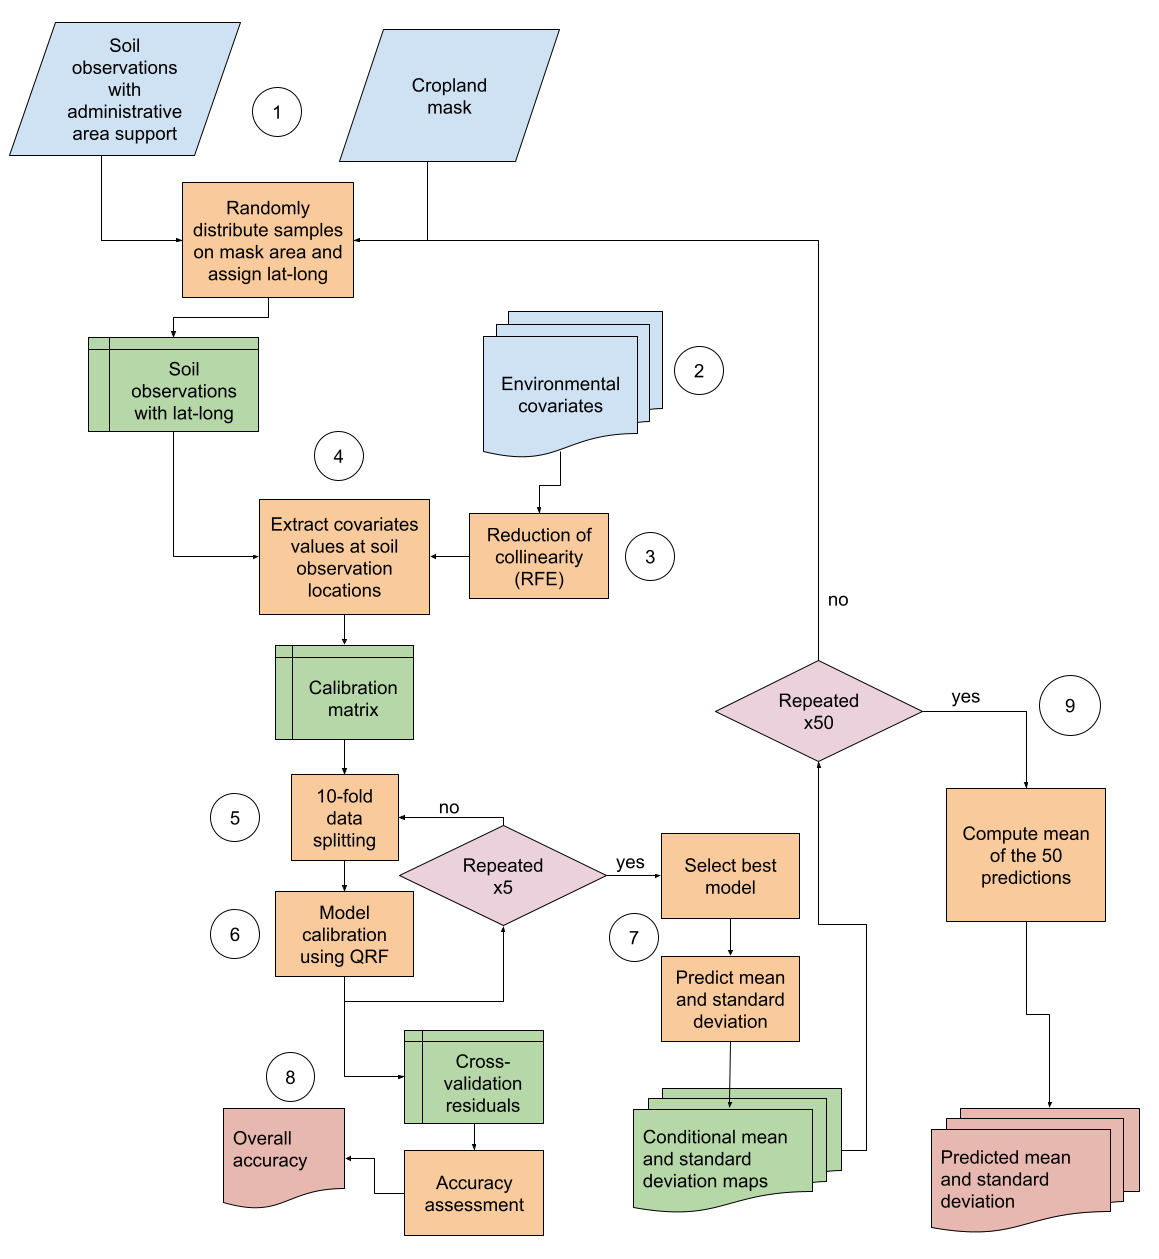
\includegraphics[width=1\linewidth]{images/workflow_county_data} \caption{Digital soil mapping approach for area-support data. Circles are the steps.}\label{fig:workflow2}
\end{figure}

The steps are similar to the ones specified in Step 3. After merging the soil and environmental covariate data, the ones with most explanatory power are selected for model calibration. The uncertainty model is then assessed and finally the target soil property predicted. This is followed by the exporting of the final map products.

First, the working directory is set, the file path to the shapefile that contains the area of interest as well as the name of the target soil property are assigned to two object. Next, the number of simulations in which the samples are repeatedly distributed by random over the respective area is specified (see Figure \ref{fig:workflow2}). Next, the saved function for uncertainty assessment is loaded as well as all packages that are needed to run the script.

\begin{Shaded}
\begin{Highlighting}[]
\CommentTok{\# 0 {-} Set working directory, soil attribute, and packages ======================}

\CommentTok{\# Working directory}
\FunctionTok{setwd}\NormalTok{(}\StringTok{\textquotesingle{}C:/GIT/GSNmap{-}TM/Digital{-}Soil{-}Mapping\textquotesingle{}}\NormalTok{)}

\CommentTok{\# Load Area of interest (shp)}
\NormalTok{AOI }\OtherTok{\textless{}{-}} \StringTok{\textquotesingle{}01{-}Data/AOI\_Arg.shp\textquotesingle{}}

\CommentTok{\# Terget soil attribute}
\NormalTok{soilatt }\OtherTok{\textless{}{-}} \StringTok{\textquotesingle{}p\_bray\textquotesingle{}}

\CommentTok{\# Repetitions (should be equal or greater than 50)}
\NormalTok{n\_sim }\OtherTok{=} \DecValTok{5}

\CommentTok{\# Function for Uncertainty Assessment}
\FunctionTok{load}\NormalTok{(}\AttributeTok{file =} \StringTok{"03{-}Scripts/eval.RData"}\NormalTok{)}

\CommentTok{\#load packages}
\FunctionTok{library}\NormalTok{(tidyverse)}
\FunctionTok{library}\NormalTok{(data.table)}
\FunctionTok{library}\NormalTok{(caret)}
\FunctionTok{library}\NormalTok{(quantregForest)}
\FunctionTok{library}\NormalTok{(terra)}
\FunctionTok{library}\NormalTok{(sf)}
\FunctionTok{library}\NormalTok{(doParallel)}
\FunctionTok{library}\NormalTok{(mapview)}
\CommentTok{\# install.packages("terra", repos = "https://rspatial.r{-}universe.dev")}
\end{Highlighting}
\end{Shaded}

In the following lines of code, the data for validation is loaded. It consists of soil data that has point coordinates. However, if no data with covariates is available, this step can be skipped.
Also, environmental covariate data are loaded and stacked together into one R object. Of this R object ``covs'', values are extracted for the soil profile locations of the validation data.
Finally, the data without coordinates are loaded.

\begin{Shaded}
\begin{Highlighting}[]
\CommentTok{\# 1 {-} Load validation data (with coordinates) if available =====================}

\NormalTok{val\_data }\OtherTok{\textless{}{-}} \FunctionTok{read\_csv}\NormalTok{(}\StringTok{"01{-}Data/data\_with\_coord.csv"}\NormalTok{) }\SpecialCharTok{\%\textgreater{}\%} 
  \FunctionTok{vect}\NormalTok{(}\AttributeTok{geom=}\FunctionTok{c}\NormalTok{(}\StringTok{"x"}\NormalTok{, }\StringTok{"y"}\NormalTok{), }\AttributeTok{crs =} \StringTok{"epsg:4326"}\NormalTok{)}

\DocumentationTok{\#\# 1.1 {-} Load covariates {-}{-}{-}{-}{-}{-}{-}{-}{-}{-}{-}{-}{-}{-}{-}{-}{-}{-}{-}{-}{-}{-}{-}{-}{-}{-}{-}{-}{-}{-}{-}{-}{-}{-}{-}{-}{-}{-}{-}{-}{-}{-}{-}{-}{-}{-}{-}{-}{-}{-}{-}{-}{-}{-}{-}}
\CommentTok{\# Single{-}band files}
\NormalTok{f }\OtherTok{\textless{}{-}} \FunctionTok{list.files}\NormalTok{(}\StringTok{"01{-}Data/covs/"}\NormalTok{, }\StringTok{".tif$"}\NormalTok{, }\AttributeTok{full.names =} \ConstantTok{TRUE}\NormalTok{)}
\NormalTok{f }\OtherTok{\textless{}{-}}\NormalTok{ f[f }\SpecialCharTok{!=}\StringTok{"01{-}Data/covs/covs.tif"}\NormalTok{]}
\NormalTok{covs }\OtherTok{\textless{}{-}} \FunctionTok{rast}\NormalTok{(f)}

\CommentTok{\# Multi{-}band file}
\CommentTok{\# covs \textless{}{-} rast("01{-}Data/covs/covs.tif")}

\CommentTok{\# extract names of covariates}
\NormalTok{ncovs }\OtherTok{\textless{}{-}} \FunctionTok{names}\NormalTok{(covs)}
\NormalTok{ncovs }\OtherTok{\textless{}{-}} \FunctionTok{str\_replace}\NormalTok{(ncovs, }\StringTok{"{-}"}\NormalTok{, }\StringTok{"\_"}\NormalTok{)}
\FunctionTok{names}\NormalTok{(covs) }\OtherTok{\textless{}{-}}\NormalTok{ ncovs}

\DocumentationTok{\#\# 1.2 {-} extract values from covariates for validation data {-}{-}{-}{-}{-}{-}{-}{-}{-}{-}{-}{-}{-}{-}{-}{-}{-}{-}{-}{-}}
\NormalTok{ex }\OtherTok{\textless{}{-}}\NormalTok{ terra}\SpecialCharTok{::}\FunctionTok{extract}\NormalTok{(}\AttributeTok{x =}\NormalTok{ covs, }\AttributeTok{y =}\NormalTok{ val\_data, }\AttributeTok{xy=}\NormalTok{F)}
\NormalTok{val\_data }\OtherTok{\textless{}{-}} \FunctionTok{as.data.frame}\NormalTok{(val\_data)}
\NormalTok{val\_data }\OtherTok{\textless{}{-}} \FunctionTok{cbind}\NormalTok{(val\_data, ex)}
\NormalTok{val\_data }\OtherTok{\textless{}{-}} \FunctionTok{na.omit}\NormalTok{(val\_data)}

\DocumentationTok{\#\# 1.3 {-} Load the soil data without coordinates {-}{-}{-}{-}{-}{-}{-}{-}{-}{-}{-}{-}{-}{-}{-}{-}{-}{-}{-}{-}{-}{-}{-}{-}{-}{-}{-}{-}{-}{-}{-}{-}}
\NormalTok{dat }\OtherTok{\textless{}{-}} \FunctionTok{read\_csv}\NormalTok{(}\StringTok{"01{-}Data/Buenos\_Aires\_sur\_P\_Bray.csv"}\NormalTok{)}
\end{Highlighting}
\end{Shaded}

The next step groups the sample by ``\emph{stratum}'', i.e.~district or other administrative unit level. The number of samples per stratum are counted and only strata with more than 5 samples retained.

\begin{Shaded}
\begin{Highlighting}[]
\CommentTok{\# Compute the number of samples per stratum }
\NormalTok{N }\OtherTok{\textless{}{-}}\NormalTok{ dat }\SpecialCharTok{\%\textgreater{}\%} \FunctionTok{group\_by}\NormalTok{(stratum) }\SpecialCharTok{\%\textgreater{}\%} 
  \FunctionTok{summarise}\NormalTok{(}\AttributeTok{N=}\FunctionTok{n}\NormalTok{()) }\SpecialCharTok{\%\textgreater{}\%} 
  \FunctionTok{na.omit}\NormalTok{()}
\CommentTok{\# remove any stratum with few samples}
\NormalTok{N }\OtherTok{\textless{}{-}}\NormalTok{ N[N}\SpecialCharTok{$}\NormalTok{N }\SpecialCharTok{\textgreater{}} \DecValTok{5}\NormalTok{,]}

\CommentTok{\# null dataframe to store model residuals}
\NormalTok{df }\OtherTok{\textless{}{-}} \ConstantTok{NULL}
\end{Highlighting}
\end{Shaded}

In the following lines of code the modelling of the target soil attribute is modelled for each stratum. First, each stratum is masked with a cropland layer and then the number of pixels is counted. Next, a number of pixels is extracted from the stratum that corresponds to the total number of samples for the area.
Within another for loop, the number of sites per stratum are selected and the user can check the exact location. Then, the selected coordinates are combined with the soil data without coordinates and the values of the environmental covariates for these points are extracted with the extract() function of the terra package.
After formulating the model formula, the model is trained and then calibrated using parallel computing. Note that cross-validation is not applied. Variable importance of the covariates is assessed and the model is saved.
The uncertainty assessment uses the validation data (if available) as observed values and the predicted values to calculated the error indices and model fit parameters explained in the Section on \protect\hyperlink{uncertainty-assessment}{Uncertainty assessment}. Finally, the point values are plotted as scatterplots and residuals are saved as a .csv file.

\begin{Shaded}
\begin{Highlighting}[]
\CommentTok{\# 2 {-} Sequentially model the soil attribute ====================================}
\ControlFlowTok{for}\NormalTok{ (i }\ControlFlowTok{in} \DecValTok{1}\SpecialCharTok{:}\NormalTok{n\_sim) \{}
  \CommentTok{\# load tif file of strata (masked by croplands)}
\NormalTok{  stratum }\OtherTok{\textless{}{-}} \FunctionTok{rast}\NormalTok{(}\StringTok{"01{-}Data/land cover/SE\_districts\_croplands.tif"}\NormalTok{)}
  \CommentTok{\# Compute the number of pixels within each stratum}
\NormalTok{  y }\OtherTok{\textless{}{-}} \FunctionTok{freq}\NormalTok{(stratum)}
  \CommentTok{\# randomly select max(N) pixels within each stratum}
\NormalTok{  x }\OtherTok{\textless{}{-}} \FunctionTok{spatSample}\NormalTok{(}\AttributeTok{x =}\NormalTok{ stratum, }\FunctionTok{max}\NormalTok{(N}\SpecialCharTok{$}\NormalTok{N), }\AttributeTok{method =} \StringTok{"stratified"}\NormalTok{,}
                  \AttributeTok{as.df=}\NormalTok{T, }\AttributeTok{xy=}\NormalTok{T, }\AttributeTok{replace=}\NormalTok{F)}
  \FunctionTok{table}\NormalTok{(x}\SpecialCharTok{$}\NormalTok{stratum)}
  \CommentTok{\# remove any stratum that is not present in the data (dat)}
\NormalTok{  x }\OtherTok{\textless{}{-}}\NormalTok{ x[x}\SpecialCharTok{$}\NormalTok{stratum }\SpecialCharTok{\%in\%}\NormalTok{ N}\SpecialCharTok{$}\NormalTok{stratum,]}
  \CommentTok{\# load data without coordinates again }
\NormalTok{  dat }\OtherTok{\textless{}{-}} \FunctionTok{read\_csv}\NormalTok{(}\StringTok{"01{-}Data/Buenos\_Aires\_sur\_P\_Bray.csv"}\NormalTok{) }\SpecialCharTok{\%\textgreater{}\%} 
    \FunctionTok{na.omit}\NormalTok{()}
  \CommentTok{\# create a vector with strata}
\NormalTok{  strata }\OtherTok{\textless{}{-}} \FunctionTok{unique}\NormalTok{(x}\SpecialCharTok{$}\NormalTok{stratum)}
  \CommentTok{\# select the corresponding number of sites per stratum}
\NormalTok{  d }\OtherTok{\textless{}{-}} \ConstantTok{NULL}
  \ControlFlowTok{for}\NormalTok{ (j }\ControlFlowTok{in} \FunctionTok{seq\_along}\NormalTok{(strata)) \{}
\NormalTok{    z }\OtherTok{\textless{}{-}}\NormalTok{ x[x}\SpecialCharTok{$}\NormalTok{stratum}\SpecialCharTok{==}\NormalTok{strata[j],]}
\NormalTok{    n }\OtherTok{\textless{}{-}}\NormalTok{ N[N}\SpecialCharTok{$}\NormalTok{stratum}\SpecialCharTok{==}\NormalTok{strata[j],}\StringTok{"N"}\NormalTok{][[}\DecValTok{1}\NormalTok{]]}
\NormalTok{    z }\OtherTok{\textless{}{-}}\NormalTok{ z[}\FunctionTok{sample}\NormalTok{(}\DecValTok{1}\SpecialCharTok{:}\FunctionTok{max}\NormalTok{(N}\SpecialCharTok{$}\NormalTok{N), }\AttributeTok{size =}\NormalTok{ n),]}
    \ControlFlowTok{if}\NormalTok{(strata[j] }\SpecialCharTok{\%in\%}\NormalTok{ dat}\SpecialCharTok{$}\NormalTok{stratum)\{}
\NormalTok{      z }\OtherTok{\textless{}{-}} \FunctionTok{cbind}\NormalTok{(z,dat[dat}\SpecialCharTok{$}\NormalTok{stratum}\SpecialCharTok{==}\NormalTok{strata[j],soilatt])}
\NormalTok{      d }\OtherTok{\textless{}{-}} \FunctionTok{rbind}\NormalTok{(d,z)\}}
\NormalTok{  \}}
  \CommentTok{\# check the distribution of points}
\NormalTok{  d }\SpecialCharTok{\%\textgreater{}\%}
    \FunctionTok{st\_as\_sf}\NormalTok{(}\AttributeTok{coords =} \FunctionTok{c}\NormalTok{(}\StringTok{"x"}\NormalTok{, }\StringTok{"y"}\NormalTok{), }\AttributeTok{crs =} \DecValTok{4326}\NormalTok{) }\SpecialCharTok{\%\textgreater{}\%} \CommentTok{\# convert to spatial object}
    \FunctionTok{mapview}\NormalTok{(}\AttributeTok{zcol =}\NormalTok{ soilatt, }\AttributeTok{cex =} \DecValTok{2}\NormalTok{, }\AttributeTok{lwd =} \FloatTok{0.1}\NormalTok{) }\CommentTok{\#+ mapview(raster(stratum))}
\NormalTok{  dat }\OtherTok{\textless{}{-}} \FunctionTok{vect}\NormalTok{(d, }\AttributeTok{geom=}\FunctionTok{c}\NormalTok{(}\StringTok{"x"}\NormalTok{, }\StringTok{"y"}\NormalTok{), }\AttributeTok{crs =} \StringTok{"epsg:4326"}\NormalTok{)}
  
  \CommentTok{\# Extract values from covariates  }
\NormalTok{  pv }\OtherTok{\textless{}{-}}\NormalTok{ terra}\SpecialCharTok{::}\FunctionTok{extract}\NormalTok{(}\AttributeTok{x =}\NormalTok{ covs, }\AttributeTok{y =}\NormalTok{ dat, }\AttributeTok{xy=}\NormalTok{F)}
\NormalTok{  dat }\OtherTok{\textless{}{-}} \FunctionTok{cbind}\NormalTok{(dat,pv)}
\NormalTok{  dat }\OtherTok{\textless{}{-}} \FunctionTok{as.data.frame}\NormalTok{(dat)}
  
  \CommentTok{\# Select from dat the soil attribute and the covariates and remove NAs}
\NormalTok{  d }\OtherTok{\textless{}{-}} \FunctionTok{select}\NormalTok{(dat, soilatt, ncovs)}
\NormalTok{  d }\OtherTok{\textless{}{-}} \FunctionTok{na.omit}\NormalTok{(d)}
  
  \CommentTok{\# formula}
\NormalTok{  fm }\OtherTok{=} \FunctionTok{as.formula}\NormalTok{(}\FunctionTok{paste}\NormalTok{(soilatt,}\StringTok{" \textasciitilde{}"}\NormalTok{, }\FunctionTok{paste0}\NormalTok{(ncovs,}
                                             \AttributeTok{collapse =} \StringTok{"+"}\NormalTok{)))}
  \CommentTok{\# parallel processing}
\NormalTok{  cl }\OtherTok{\textless{}{-}} \FunctionTok{makeCluster}\NormalTok{(}\FunctionTok{detectCores}\NormalTok{()}\SpecialCharTok{{-}}\DecValTok{1}\NormalTok{)}
  \FunctionTok{registerDoParallel}\NormalTok{(cl)}
  
  \CommentTok{\# Set training parameters (CV is not applied)}
\NormalTok{  fitControl }\OtherTok{\textless{}{-}} \FunctionTok{trainControl}\NormalTok{(}\AttributeTok{method =} \StringTok{"none"}\NormalTok{,}
                             \CommentTok{\# number = 10,         \#\# 10 {-}fold CV}
                             \CommentTok{\# repeats = 3,        \#\# repeated 3 times}
                             \AttributeTok{savePredictions =} \ConstantTok{TRUE}\NormalTok{)}
  
  \CommentTok{\# Tune mtry hyperparameter}
\NormalTok{  mtry }\OtherTok{\textless{}{-}} \FunctionTok{round}\NormalTok{(}\FunctionTok{length}\NormalTok{(ncovs)}\SpecialCharTok{/}\DecValTok{3}\NormalTok{)}
\NormalTok{  tuneGrid }\OtherTok{\textless{}{-}}  \FunctionTok{expand.grid}\NormalTok{(}\AttributeTok{mtry =} \FunctionTok{c}\NormalTok{(mtry))}
  
  \CommentTok{\# Calibrate the QRF model }
  \FunctionTok{print}\NormalTok{(}\FunctionTok{paste}\NormalTok{(}\StringTok{"start fitting model"}\NormalTok{, i))}
\NormalTok{  model }\OtherTok{\textless{}{-}}\NormalTok{ caret}\SpecialCharTok{::}\FunctionTok{train}\NormalTok{(fm,}
                        \AttributeTok{data =}\NormalTok{ d,}
                        \AttributeTok{method =} \StringTok{"qrf"}\NormalTok{,}
                        \AttributeTok{trControl =}\NormalTok{ fitControl,}
                        \AttributeTok{verbose =} \ConstantTok{TRUE}\NormalTok{,}
                        \AttributeTok{tuneGrid =}\NormalTok{ tuneGrid,}
                        \AttributeTok{keep.inbag =}\NormalTok{ T,}
                        \AttributeTok{importance =} \ConstantTok{TRUE}\NormalTok{, )}
  \FunctionTok{stopCluster}\NormalTok{(cl)}
  \FunctionTok{gc}\NormalTok{()}
  \FunctionTok{print}\NormalTok{(}\FunctionTok{paste}\NormalTok{(}\StringTok{"end fitting"}\NormalTok{, i))}
  \CommentTok{\# Extract predictor importance }
\NormalTok{  x }\OtherTok{\textless{}{-}}\NormalTok{ randomForest}\SpecialCharTok{::}\FunctionTok{importance}\NormalTok{(model}\SpecialCharTok{$}\NormalTok{finalModel)}
\NormalTok{  model}\SpecialCharTok{$}\NormalTok{importance }\OtherTok{\textless{}{-}}\NormalTok{ x}
  \CommentTok{\# Plot Covariate importance }
\NormalTok{  (g2 }\OtherTok{\textless{}{-}} \FunctionTok{varImpPlot}\NormalTok{(model}\SpecialCharTok{$}\NormalTok{finalModel, }\AttributeTok{main =}\NormalTok{ soilatt, }\AttributeTok{type =} \DecValTok{1}\NormalTok{))}
  \CommentTok{\# Save the plot if you like}
  \CommentTok{\# png(filename = paste0("02{-}Outputs/importance\_",soilatt,"\_",i,".png"), }
  \CommentTok{\#     width = 15, height = 15, units = "cm", res = 600)}
  \CommentTok{\# g2}
  \CommentTok{\# dev.off()}
  \CommentTok{\# Print and save model }
  \FunctionTok{print}\NormalTok{(model)}
  \FunctionTok{saveRDS}\NormalTok{(model, }\AttributeTok{file =} \FunctionTok{paste0}\NormalTok{(}\StringTok{"02{-}Outputs/models/model\_"}\NormalTok{,soilatt,}\StringTok{"\_"}\NormalTok{,i,}\StringTok{".rds"}\NormalTok{))}
  
  \CommentTok{\# Uncertainty assessment }
  \CommentTok{\# extract observed and predicted values}
\NormalTok{  o }\OtherTok{\textless{}{-}}\NormalTok{ val\_data[,soilatt]}
\NormalTok{  p }\OtherTok{\textless{}{-}} \FunctionTok{predict}\NormalTok{(model}\SpecialCharTok{$}\NormalTok{finalModel, val\_data, }\AttributeTok{what =}\NormalTok{ mean)}
\NormalTok{  df }\OtherTok{\textless{}{-}} \FunctionTok{rbind}\NormalTok{(df, }\FunctionTok{data.frame}\NormalTok{(o,p, }\AttributeTok{model=}\NormalTok{i))}
  \CommentTok{\# Print accuracy coeficients }
  \CommentTok{\# https://github.com/AlexandreWadoux/MapQualityEvaluation}
  \FunctionTok{print}\NormalTok{(}\FunctionTok{paste}\NormalTok{(}\StringTok{"model"}\NormalTok{, i))}
  \FunctionTok{print}\NormalTok{(}\FunctionTok{eval}\NormalTok{(p,o))}
  
  \CommentTok{\# Plot and save scatterplot }
\NormalTok{  (g1 }\OtherTok{\textless{}{-}} \FunctionTok{ggplot}\NormalTok{(df, }\FunctionTok{aes}\NormalTok{(}\AttributeTok{x =}\NormalTok{ o, }\AttributeTok{y =}\NormalTok{ p)) }\SpecialCharTok{+} 
     \FunctionTok{geom\_point}\NormalTok{(}\AttributeTok{alpha =} \FloatTok{0.5}\NormalTok{) }\SpecialCharTok{+} 
     \FunctionTok{geom\_abline}\NormalTok{(}\AttributeTok{slope =} \DecValTok{1}\NormalTok{, }\AttributeTok{intercept =} \DecValTok{0}\NormalTok{, }\AttributeTok{color =} \StringTok{"red"}\NormalTok{)}\SpecialCharTok{+}
     \FunctionTok{ylim}\NormalTok{(}\FunctionTok{c}\NormalTok{(}\FunctionTok{min}\NormalTok{(o), }\FunctionTok{max}\NormalTok{(o))) }\SpecialCharTok{+} \FunctionTok{theme}\NormalTok{(}\AttributeTok{aspect.ratio=}\DecValTok{1}\NormalTok{)}\SpecialCharTok{+} 
     \FunctionTok{labs}\NormalTok{(}\AttributeTok{title =}\NormalTok{ soilatt) }\SpecialCharTok{+} 
     \FunctionTok{xlab}\NormalTok{(}\StringTok{"Observed"}\NormalTok{) }\SpecialCharTok{+} \FunctionTok{ylab}\NormalTok{(}\StringTok{"Predicted"}\NormalTok{))}
  
  \CommentTok{\# save the plots if you like}
  \CommentTok{\# ggsave(g1, filename = paste0("02{-}Outputs/residuals\_",soilatt,"\_",i,".png"), }
  \CommentTok{\#        scale = 1,}
  \CommentTok{\#        units = "cm", width = 12, height = 12)}
  
\NormalTok{\}}
\FunctionTok{write\_csv}\NormalTok{(df, }\FunctionTok{paste}\NormalTok{(}\StringTok{"residuals\_"}\NormalTok{,soilatt,}\StringTok{".csv"}\NormalTok{))}
\end{Highlighting}
\end{Shaded}

The previous model fitting and calibration is simulated 5 times, as specified at the beginning of the script. In the following part of the script, the conditional mean and standard deviation are predicted for each simulation. For that, the study area is divided into tiles. For each tile, the respective covariates and models (saved in the previous step) are used to predict mean and standard deviation which are then stored in two separate raster files.

\begin{Shaded}
\begin{Highlighting}[]
\CommentTok{\# 3 {-} Prediction ===============================================================}
\CommentTok{\# Predict conditional mean and standard deviation for each n\_sim  }
\DocumentationTok{\#\# 3.1 {-} Produce tiles {-}{-}{-}{-}{-}{-}{-}{-}{-}{-}{-}{-}{-}{-}{-}{-}{-}{-}{-}{-}{-}{-}{-}{-}{-}{-}{-}{-}{-}{-}{-}{-}{-}{-}{-}{-}{-}{-}{-}{-}{-}{-}{-}{-}{-}{-}{-}{-}{-}{-}{-}{-}{-}{-}{-}{-}{-}}
\NormalTok{r }\OtherTok{\textless{}{-}}\NormalTok{ covs[[}\DecValTok{1}\NormalTok{]]}
\CommentTok{\# adjust the number of tiles according to the size and shape of your study area}
\NormalTok{t }\OtherTok{\textless{}{-}} \FunctionTok{rast}\NormalTok{(}\AttributeTok{nrows =} \DecValTok{5}\NormalTok{, }\AttributeTok{ncols =} \DecValTok{5}\NormalTok{, }\AttributeTok{extent =} \FunctionTok{ext}\NormalTok{(r), }\AttributeTok{crs =} \FunctionTok{crs}\NormalTok{(r))}
\NormalTok{tile }\OtherTok{\textless{}{-}} \FunctionTok{makeTiles}\NormalTok{(r, t,}\AttributeTok{overwrite=}\ConstantTok{TRUE}\NormalTok{,}\AttributeTok{filename=}\StringTok{"02{-}Outputs/tiles/tiles.tif"}\NormalTok{)}

\DocumentationTok{\#\# 3.2 {-} Predict soil attributes per tiles {-}{-}{-}{-}{-}{-}{-}{-}{-}{-}{-}{-}{-}{-}{-}{-}{-}{-}{-}{-}{-}{-}{-}{-}{-}{-}{-}{-}{-}{-}{-}{-}{-}{-}{-}{-}{-}}
\CommentTok{\# loop to predict on each tile for each simulation (n tiles x n simulation)}
\ControlFlowTok{for}\NormalTok{ (j }\ControlFlowTok{in} \FunctionTok{seq\_along}\NormalTok{(tile)) \{}
  \CommentTok{\# where j is the number of tile}
  \ControlFlowTok{for}\NormalTok{ (i }\ControlFlowTok{in} \DecValTok{1}\SpecialCharTok{:}\NormalTok{n\_sim) \{}
    \CommentTok{\# where i is the number of simulation}
    \FunctionTok{gc}\NormalTok{()}
    \CommentTok{\# Read the tile j}
\NormalTok{    t }\OtherTok{\textless{}{-}} \FunctionTok{rast}\NormalTok{(tile[j])}
    \CommentTok{\# crop the covs with the tile extent}
\NormalTok{    covst }\OtherTok{\textless{}{-}} \FunctionTok{crop}\NormalTok{(covs, t)}
    \CommentTok{\# read the model i}
\NormalTok{    model }\OtherTok{\textless{}{-}} \FunctionTok{readRDS}\NormalTok{(}\FunctionTok{paste0}\NormalTok{(}\StringTok{"02{-}Outputs/models/model\_"}\NormalTok{,soilatt,}\StringTok{"\_"}\NormalTok{, i,}\StringTok{".rds"}\NormalTok{))}
    \CommentTok{\# predict mean and sd}
\NormalTok{    meanFunc }\OtherTok{=} \ControlFlowTok{function}\NormalTok{(x) }\FunctionTok{mean}\NormalTok{(x, }\AttributeTok{na.rm=}\ConstantTok{TRUE}\NormalTok{)}
\NormalTok{    pred\_mean }\OtherTok{\textless{}{-}}\NormalTok{ terra}\SpecialCharTok{::}\FunctionTok{predict}\NormalTok{(covst, }\AttributeTok{model =}\NormalTok{ model}\SpecialCharTok{$}\NormalTok{finalModel, }\AttributeTok{na.rm =} \ConstantTok{TRUE}\NormalTok{,   }
                                \AttributeTok{cpkgs=}\StringTok{"quantregForest"}\NormalTok{, }\AttributeTok{what=}\NormalTok{meanFunc)}
\NormalTok{    sdFunc }\OtherTok{=} \ControlFlowTok{function}\NormalTok{(x) }\FunctionTok{sd}\NormalTok{(x, }\AttributeTok{na.rm=}\ConstantTok{TRUE}\NormalTok{)}
\NormalTok{    pred\_sd }\OtherTok{\textless{}{-}}\NormalTok{ terra}\SpecialCharTok{::}\FunctionTok{predict}\NormalTok{(covst, }\AttributeTok{model =}\NormalTok{ model}\SpecialCharTok{$}\NormalTok{finalModel, }\AttributeTok{na.rm=}\ConstantTok{TRUE}\NormalTok{,  }
                              \AttributeTok{cpkgs=}\StringTok{"quantregForest"}\NormalTok{, }\AttributeTok{what=}\NormalTok{sdFunc)  }
    \CommentTok{\# save the predicted tiles}
    \FunctionTok{writeRaster}\NormalTok{(pred\_mean, }
                \AttributeTok{filename =} \FunctionTok{paste0}\NormalTok{(}\StringTok{"02{-}Outputs/tiles/soilatt\_tiles/"}\NormalTok{,}
\NormalTok{                                  soilatt,}\StringTok{"\_tile\_"}\NormalTok{, j,}\StringTok{"\_model\_"}\NormalTok{,i,}\StringTok{".tif"}\NormalTok{), }
                \AttributeTok{overwrite =} \ConstantTok{TRUE}\NormalTok{)}
    \FunctionTok{writeRaster}\NormalTok{(pred\_sd, }
                \AttributeTok{filename =} \FunctionTok{paste0}\NormalTok{(}\StringTok{"02{-}Outputs/tiles/soilatt\_tiles/"}\NormalTok{,}
\NormalTok{                                  soilatt,}\StringTok{"\_tileSD\_"}\NormalTok{, j,}\StringTok{"\_model\_"}\NormalTok{,i,}\StringTok{".tif"}\NormalTok{), }
                \AttributeTok{overwrite =} \ConstantTok{TRUE}\NormalTok{)}
    
    \FunctionTok{rm}\NormalTok{(pred\_mean)}
    \FunctionTok{rm}\NormalTok{(pred\_sd)}
    \FunctionTok{print}\NormalTok{(}\FunctionTok{paste}\NormalTok{(tile[j],}\StringTok{"model"}\NormalTok{, i))}
\NormalTok{  \}}
\NormalTok{\}}
\end{Highlighting}
\end{Shaded}

Eventually, the predicted tiles are merged for each simulation (one for mean, one for standard deviation). Finally, two raster files are saved.

\begin{Shaded}
\begin{Highlighting}[]
\DocumentationTok{\#\# 3.3 {-} Merge tiles both prediction and st.Dev for each simulation {-}{-}{-}{-}{-}{-}{-}{-}{-}{-}{-}{-}}
\ControlFlowTok{for}\NormalTok{ (j }\ControlFlowTok{in} \FunctionTok{seq\_along}\NormalTok{(tile)) \{}
  \CommentTok{\# merge tiles of simulation j}
\NormalTok{  f\_mean }\OtherTok{\textless{}{-}} \FunctionTok{list.files}\NormalTok{(}\AttributeTok{path =} \StringTok{"02{-}Outputs/tiles/soilatt\_tiles/"}\NormalTok{, }
                       \AttributeTok{pattern =} \FunctionTok{paste0}\NormalTok{(soilatt,}\StringTok{"\_tile\_"}\NormalTok{,j,}\StringTok{"\_model\_"}\NormalTok{), }
                       \AttributeTok{full.names =} \ConstantTok{TRUE}\NormalTok{)}
\NormalTok{  f\_sd }\OtherTok{\textless{}{-}} \FunctionTok{list.files}\NormalTok{(}\AttributeTok{path =} \StringTok{"02{-}Outputs/tiles/soilatt\_tiles/"}\NormalTok{, }
                     \AttributeTok{pattern =}  \FunctionTok{paste0}\NormalTok{(soilatt,}\StringTok{"\_tileSD\_"}\NormalTok{,j,}\StringTok{"\_model\_"}\NormalTok{), }
                     \AttributeTok{full.names =} \ConstantTok{TRUE}\NormalTok{)}
  \CommentTok{\# Estimate the mean of the n\_sim predictions (both mean and sd) for each tile}
\NormalTok{  pred\_mean }\OtherTok{\textless{}{-}} \FunctionTok{rast}\NormalTok{(f\_mean) }\SpecialCharTok{\%\textgreater{}\%} \FunctionTok{mean}\NormalTok{(}\AttributeTok{na.rm=}\ConstantTok{TRUE}\NormalTok{)}
\NormalTok{  pred\_sd }\OtherTok{\textless{}{-}} \FunctionTok{rast}\NormalTok{(f\_sd) }\SpecialCharTok{\%\textgreater{}\%} \FunctionTok{mean}\NormalTok{(}\AttributeTok{na.rm=}\ConstantTok{TRUE}\NormalTok{)}
  \FunctionTok{names}\NormalTok{(pred\_sd) }\OtherTok{\textless{}{-}} \StringTok{"sd"}
  \CommentTok{\# save resulting tiles}
  \FunctionTok{writeRaster}\NormalTok{(pred\_sd, }
              \AttributeTok{filename =} \FunctionTok{paste0}\NormalTok{(}\StringTok{"02{-}Outputs/tiles/aggregated\_tiles/"}\NormalTok{,}
\NormalTok{                                soilatt,}\StringTok{"\_tilesd\_"}\NormalTok{, j,}\StringTok{".tif"}\NormalTok{), }
              \AttributeTok{overwrite =} \ConstantTok{TRUE}\NormalTok{)}
  \FunctionTok{writeRaster}\NormalTok{(pred\_mean, }
              \AttributeTok{filename =} \FunctionTok{paste0}\NormalTok{(}\StringTok{"02{-}Outputs/tiles/aggregated\_tiles/"}\NormalTok{,}
\NormalTok{                                soilatt,}\StringTok{"\_tileMean\_"}\NormalTok{, j,}\StringTok{".tif"}\NormalTok{), }
              \AttributeTok{overwrite =} \ConstantTok{TRUE}\NormalTok{)}
  \FunctionTok{print}\NormalTok{(j)}
\NormalTok{\}}
\end{Highlighting}
\end{Shaded}

In the following, the tiles are merged to one file that is outputted as raster file and saved in the maps folder.

\begin{Shaded}
\begin{Highlighting}[]
\DocumentationTok{\#\# 3.4 {-} Merge tiles {-}{-}{-}{-}{-}{-}{-}{-}{-}{-}{-}{-}{-}{-}{-}{-}{-}{-}{-}{-}{-}{-}{-}{-}{-}{-}{-}{-}{-}{-}{-}{-}{-}{-}{-}{-}{-}{-}{-}{-}{-}{-}{-}{-}{-}{-}{-}{-}{-}{-}{-}{-}{-}{-}{-}{-}{-}{-}{-} }
\NormalTok{name\_tiles }\OtherTok{\textless{}{-}} \FunctionTok{c}\NormalTok{(}\StringTok{"sd"}\NormalTok{, }\StringTok{"Mean"}\NormalTok{)}
\ControlFlowTok{for}\NormalTok{ (i }\ControlFlowTok{in} \FunctionTok{seq\_along}\NormalTok{(name\_tiles)) \{}
  \CommentTok{\# list tiles }
\NormalTok{  f }\OtherTok{\textless{}{-}} \FunctionTok{list.files}\NormalTok{(}\AttributeTok{path =} \StringTok{"02{-}Outputs/tiles/aggregated\_tiles/"}\NormalTok{, }
                  \AttributeTok{pattern =} \FunctionTok{paste0}\NormalTok{(soilatt,}\StringTok{"\_tile"}\NormalTok{,name\_tiles[i]), }
                  \AttributeTok{full.names =} \ConstantTok{TRUE}\NormalTok{)}
  \CommentTok{\# read tiles}
\NormalTok{  r }\OtherTok{\textless{}{-}} \FunctionTok{list}\NormalTok{()}
  \ControlFlowTok{for}\NormalTok{ (g }\ControlFlowTok{in} \FunctionTok{seq\_along}\NormalTok{(f))\{}
\NormalTok{    r[[g]] }\OtherTok{\textless{}{-}} \FunctionTok{rast}\NormalTok{(f[g])}
    \FunctionTok{print}\NormalTok{(g)}
\NormalTok{  \}}
  \CommentTok{\# Mosaic tiles}
\NormalTok{  r }\OtherTok{\textless{}{-}} \FunctionTok{sprc}\NormalTok{(r)}
\NormalTok{  r }\OtherTok{\textless{}{-}} \FunctionTok{mosaic}\NormalTok{(r)}
  \CommentTok{\# plot final map}
  \FunctionTok{plot}\NormalTok{(r, }\AttributeTok{main =} \FunctionTok{paste}\NormalTok{(}\StringTok{"Predicted"}\NormalTok{,name\_tiles[i]))}
  \CommentTok{\# save final map}
  \FunctionTok{writeRaster}\NormalTok{(r, }\FunctionTok{paste0}\NormalTok{(}\StringTok{"02{-}Outputs/maps/"}\NormalTok{,soilatt,name\_tiles[i],}\StringTok{".tif"}\NormalTok{),}
              \AttributeTok{overwrite=}\ConstantTok{TRUE}\NormalTok{)}
  \FunctionTok{rm}\NormalTok{(r)}
  \FunctionTok{gc}\NormalTok{()}
\NormalTok{\}}
\end{Highlighting}
\end{Shaded}

In case data with coordinates is available, the eval function is employed at the end to assess the gap between observed values with coordinates and the predicted ones without area-support.

\begin{Shaded}
\begin{Highlighting}[]
\CommentTok{\# 4 {-} Validate resulting map ===================================================}
\CommentTok{\# Load data with coordinates}
\NormalTok{val\_data }\OtherTok{\textless{}{-}} \FunctionTok{read\_csv}\NormalTok{(}\StringTok{"01{-}Data/data\_with\_coord.csv"}\NormalTok{) }\SpecialCharTok{\%\textgreater{}\%} 
  \FunctionTok{vect}\NormalTok{(}\AttributeTok{geom=}\FunctionTok{c}\NormalTok{(}\StringTok{"x"}\NormalTok{, }\StringTok{"y"}\NormalTok{), }\AttributeTok{crs =} \StringTok{"epsg:4326"}\NormalTok{)}
\CommentTok{\# Load predited mean}
\NormalTok{pred\_mean }\OtherTok{\textless{}{-}} \FunctionTok{rast}\NormalTok{(}\StringTok{"02{-}Outputs/maps/p\_brayMean.tif"}\NormalTok{)}
\FunctionTok{plot}\NormalTok{(pred\_mean)}
\CommentTok{\# extract values from predicted mean map}
\NormalTok{ex }\OtherTok{\textless{}{-}}\NormalTok{ terra}\SpecialCharTok{::}\FunctionTok{extract}\NormalTok{(}\AttributeTok{x =}\NormalTok{ pred\_mean, }\AttributeTok{y =}\NormalTok{ val\_data, }\AttributeTok{xy=}\NormalTok{F, }\AttributeTok{ID=}\ConstantTok{FALSE}\NormalTok{)}
\CommentTok{\# Estimate accuracy indicators}
\NormalTok{val\_data }\OtherTok{\textless{}{-}} \FunctionTok{as.data.frame}\NormalTok{(val\_data)}
\NormalTok{val\_data }\OtherTok{\textless{}{-}} \FunctionTok{cbind}\NormalTok{(val\_data, ex)}
\NormalTok{val\_data }\OtherTok{\textless{}{-}} \FunctionTok{na.omit}\NormalTok{(val\_data)}

\FunctionTok{eval}\NormalTok{(val\_data}\SpecialCharTok{$}\NormalTok{mean,val\_data[,soilatt])}
\end{Highlighting}
\end{Shaded}

At the end of the script, the files are again masked with the cropland mask layer and saved as raster files in the maps-output folder.

\begin{Shaded}
\begin{Highlighting}[]
\CommentTok{\# 5 {-} Export final maps ========================================================}
\DocumentationTok{\#\# 5.1 {-} Mask croplands {-}{-}{-}{-}{-}{-}{-}{-}{-}{-}{-}{-}{-}{-}{-}{-}{-}{-}{-}{-}{-}{-}{-}{-}{-}{-}{-}{-}{-}{-}{-}{-}{-}{-}{-}{-}{-}{-}{-}{-}{-}{-}{-}{-}{-}{-}{-}{-}{-}{-}{-}{-}{-}{-}{-}{-}}
\NormalTok{msk }\OtherTok{\textless{}{-}} \FunctionTok{rast}\NormalTok{(}\StringTok{"01{-}Data/mask\_arg.tif"}\NormalTok{)}
\FunctionTok{plot}\NormalTok{(msk)}
\CommentTok{\# Mask croplands in predicted mean}
\NormalTok{pred\_mean }\OtherTok{\textless{}{-}} \FunctionTok{rast}\NormalTok{(}\StringTok{"02{-}Outputs/maps/p\_brayMean.tif"}\NormalTok{)}
\NormalTok{pred\_mean }\OtherTok{\textless{}{-}} \FunctionTok{mask}\NormalTok{(pred\_mean, msk)}
\FunctionTok{plot}\NormalTok{(pred\_mean)}
\CommentTok{\# Mask croplands in predicted sd}
\NormalTok{pred\_sd }\OtherTok{\textless{}{-}} \FunctionTok{rast}\NormalTok{(}\StringTok{"02{-}Outputs/maps/p\_braysd.tif"}\NormalTok{)}
\NormalTok{pred\_sd }\OtherTok{\textless{}{-}} \FunctionTok{mask}\NormalTok{(pred\_sd, msk)}
\FunctionTok{plot}\NormalTok{(pred\_sd)}

\DocumentationTok{\#\# 5.2 {-} Save results {-}{-}{-}{-}{-}{-}{-}{-}{-}{-}{-}{-}{-}{-}{-}{-}{-}{-}{-}{-}{-}{-}{-}{-}{-}{-}{-}{-}{-}{-}{-}{-}{-}{-}{-}{-}{-}{-}{-}{-}{-}{-}{-}{-}{-}{-}{-}{-}{-}{-}{-}{-}{-}{-}{-}{-}{-}{-}}
\FunctionTok{writeRaster}\NormalTok{(pred\_mean, }
            \FunctionTok{paste0}\NormalTok{(}\StringTok{"02{-}Outputs/maps/"}\NormalTok{,soilatt,}\StringTok{"\_no\_coord.tif"}\NormalTok{),}
            \AttributeTok{overwrite=}\ConstantTok{TRUE}\NormalTok{)}
\FunctionTok{writeRaster}\NormalTok{(pred\_sd, }
            \FunctionTok{paste0}\NormalTok{(}\StringTok{"02{-}Outputs/maps/"}\NormalTok{,soilatt,}\StringTok{"\_no\_coord\_SD.tif"}\NormalTok{),}
            \AttributeTok{overwrite=}\ConstantTok{TRUE}\NormalTok{)}
\end{Highlighting}
\end{Shaded}

\hypertarget{annex-iv-quality-assurance-and-quality-control}{%
\chapter*{Annex IV: Quality assurance and quality control}\label{annex-iv-quality-assurance-and-quality-control}}
\addcontentsline{toc}{chapter}{Annex IV: Quality assurance and quality control}

The following protocol was devised to provide National Experts with a step-by-step guideline to perform a Quality Assurance (QA) and Quality Control (QC) of the 10 GSNmap first phase products.

The following protocol does not provide any guidance in terms of uncertainty estimation and validation. For more details and information on the estimation of uncertainties and potential map validation strategies please refer to Chapter 8.4.

Quality assurance and quality control consist of activities to ensure the quality of a particular result. Quality control is a reactive process that focuses on identifying defects and errors while quality assurance is a proactive approach aimed at preventing defects and errors. In the context of digital soil mapping, both processes are often interlinked. A QA is interlinked with a QC when it identifies defects and the QA remodels the process to eliminate the defects and prevent them from recurring (Chapman, 2005)(Figure\ref{fig:qaqc}).

\begin{figure}
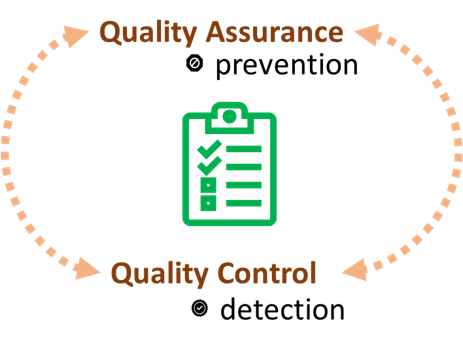
\includegraphics[width=6.43in]{images/QA_QC} \caption{Quality assurance and quality control.}\label{fig:qaqc}
\end{figure}

Each step in the following protocol should be considered in order to detect and eliminate errors, address data inaccuracies and assess the output completeness.

\hypertarget{step-1-completeness-of-layers}{%
\section*{Step 1: Completeness of layers}\label{step-1-completeness-of-layers}}
\addcontentsline{toc}{section}{Step 1: Completeness of layers}

The following Table \ref(tab:products) gives an overview of all the GSNmap products in alphabetical order. Each product should include the ISO 3166-1 alpha-3 country code as uppercase letters in its name. For instance, in the case of Turkiye, ISO\_GSNmap\_Ntot\_Map030 should be changed to TUR\_GSNmap\_Ntot\_Map030.

All 10 soil property and soil nutrient maps with their corresponding 10 uncertainty layers must be georeferenced TIF (.tif) files.

\begin{table}

\caption{\label{tab:products}\label{tab:products}Data product overview.}
\centering
\fontsize{7}{9}\selectfont
\begin{tabular}[t]{ll}
\toprule
Product & Filename\\
\midrule
\addlinespace[0.3em]
\multicolumn{2}{l}{\textbf{Major nutrients (3 files)}}\\
\hspace{1em}Total Nitrogen map & ISO\_GSNmap\_Ntot\_Map030.tiff\\
\hspace{1em}Available Phosphorus map & ISO\_GSNmap\_Pav\_Map030.tiff\\
\hspace{1em}Total Potassium map & ISO\_GSNmap\_Ktot\_Map030.tiff\\
\addlinespace[0.3em]
\multicolumn{2}{l}{\textbf{Associated soil properties (7 files)}}\\
\hspace{1em}Cation exchange capacity map & ISO\_GSNmap\_CEC\_Map030.tiff\\
\hspace{1em}Soil pH map & ISO\_GSNmap\_pH\_Map030.tiff\\
\hspace{1em}Soil clay map & ISO\_GSNmap\_Clay\_Map030.tiff\\
\hspace{1em}Soil silt map & ISO\_GSNmap\_Silt\_Map030.tiff\\
\hspace{1em}Soil sand map & ISO\_GSNmap\_Sand\_Map030.tiff\\
\hspace{1em}Soil organic carbon map & ISO\_GSNmap\_SOC\_Map030.tiff\\
\hspace{1em}Soil bulk density map & ISO\_GSNmap\_BD\_Map030.tiff\\
\addlinespace[0.3em]
\multicolumn{2}{l}{\textbf{Uncertainty maps (10 files)}}\\
\hspace{1em}Total Nitrogen uncertainty map & ISO\_GSNmap\_Ntot\_UncertaintyMap030.tiff\\
\hspace{1em}Available Phosphorus uncertainty map & ISO\_GSNmap\_Pav\_UncertaintyMap030.tiff\\
\hspace{1em}Total Potassium uncertainty map & ISO\_GSNmap\_Ktot\_UncertaintyMap030.tiff\\
\hspace{1em}Cation exchange capacity uncertainty map & ISO\_GSNmap\_CEC\_UncertaintyMap030.tiff\\
\hspace{1em}Soil pH uncertainty map & ISO\_GSNmap\_pH\_UncertaintyMap030.tiff\\
\hspace{1em}Soil clay uncertainty map & ISO\_GSNmap\_Clay\_UncertaintyMap030.tiff\\
\hspace{1em}Soil silt uncertainty map & ISO\_GSNmap\_Silt\_UncertaintyMap030.tiff\\
\hspace{1em}Soil sand uncertainty map & ISO\_GSNmap\_Sand\_UncertaintyMap030.tiff\\
\hspace{1em}Soil organic carbon uncertainty map & ISO\_GSNmap\_SOC\_UncertaintyMap030.tiff\\
\hspace{1em}Soil bulk density uncertainty map & ISO\_GSNmap\_BD\_UncertaintyMap030.tiff\\
\bottomrule
\end{tabular}
\end{table}

\hypertarget{step-2-check-the-projection-and-resolution-of-all-data-products}{%
\section*{Step 2: Check the projection and resolution of all data products}\label{step-2-check-the-projection-and-resolution-of-all-data-products}}
\addcontentsline{toc}{section}{Step 2: Check the projection and resolution of all data products}

Open the products in QGIS or any other preferred GIS platform. Check that the projection of all products is EPSG:4326 - WGS 84 (Layer properties). Check that the spatial resolution (pixel size) (Layer properties) is equal to \textasciitilde0.002246 degrees ; 250 m x 250 m at the equator.

\hypertarget{step-3-check-the-extent}{%
\section*{Step 3: Check the extent}\label{step-3-check-the-extent}}
\addcontentsline{toc}{section}{Step 3: Check the extent}

Visualize the 20 products in QGIS or any preferred GIS platform. Load a land-use layer to visually assess that the simulations were done exclusively on croplands.

\hypertarget{step-4-check-the-units-ranges-and-outliers}{%
\section*{Step 4: Check the units, ranges, and outliers}\label{step-4-check-the-units-ranges-and-outliers}}
\addcontentsline{toc}{section}{Step 4: Check the units, ranges, and outliers}

In the following section possible value ranges for each product category (except available potassium) are presented. It is important to note that the provided ranges represent a gross approximation of the extremes within which the values should fall in. Results that fall outside these ranges need to be carefully evaluated based on local expertise and available literature.

The provided ranges can be compared in QGIS, R, or any preferred platform. Descriptive layer statistics can be viewed in QGIS under Layer Properties.

The following table (Table 10.2) presents ranges of possible values for 9 of the 10 mandatory GSNmap products. The ranges were calculated based on the distribution of the soil profile data within the World Soil Information Service (WoSIS), specifically the WoSIS snapshot 2019 (Batjes, N. H. \emph{et al.} 2020). It is important to note that the data was not filtered for croplands and that the ranges were extracted from soil profiles sampled globally from a wide array of land covers and land uses.

\begin{table}

\caption{\label{tab:ranges}\label{tab:ranges}Possible soil property and soil nutrient values based on the distribution of the values within the World Soil Information Service (WoSIS), specifically the WoSIS snapshot 2019.}
\centering
\fontsize{7}{9}\selectfont
\begin{tabular}[t]{lllrrrrrr}
\toprule
Soil property & property\_id & Unit & Min & 1st Quartile & Median & 3st Quartile & Max & n\\
\midrule
Total N & n\_0\_30 & ppm & 0.0 & 400.0 & 700.0 & 1500.0 & 84000.0 & 216362\\
P Bray I & p\_0\_30 & ppm & 0.0 & 1.6 & 5.0 & 16.0 & 150.0 & 40486\\
P Mehlich 3 & p\_0\_30 & ppm & 0.0 & 1.6 & 6.1 & 22.0 & 149.4 & 7242\\
P Olsen & p\_0\_30 & ppm & 0.0 & 0.7 & 2.0 & 4.3 & 141.0 & 8434\\
CEC & cec\_0\_30 & cmol(c)/kg & 0.1 & 7.5 & 14.0 & 23.0 & 140.0 & 295688\\
\addlinespace
pH (water) & ph\_0\_30 & / & 1.5 & 5.2 & 6.2 & 7.5 & 12.3 & 613322\\
Clay & clay\_0\_30 & \% & 0.0 & 11.1 & 21.9 & 35.3 & 100.0 & 590368\\
Silt & silt\_0\_30 & \% & 0.0 & 15.0 & 30.0 & 47.6 & 100.0 & 558233\\
Sand & sand\_0\_30 & \% & 0.0 & 15.0 & 36.0 & 60.2 & 100.0 & 482334\\
Soil Organic Carbon & soc\_0\_30 & \% & 0.0 & 2.0 & 5.1 & 14.0 & 99.4 & 471301\\
\addlinespace
Bulk density & bd\_0\_30 & g/cm3 & 0.0 & 1.3 & 1.4 & 1.7 & 2.6 & 116756\\
Available K & k\_0\_30 & ppm & NA & NA & NA & NA & NA & NA\\
\bottomrule
\end{tabular}
\end{table}

\hypertarget{qaqc-script}{%
\section*{QA/QC Script}\label{qaqc-script}}
\addcontentsline{toc}{section}{QA/QC Script}

The following script automates the for Steps described in the previous sections. It is important to note that the script's main objective is to provide a fast alternative to check the output layers and that it does not replace the need to visually assess the final maps based on expert knowledge.

\begin{Shaded}
\begin{Highlighting}[]
\CommentTok{\#\_\_\_\_\_\_\_\_\_\_\_\_\_\_\_\_\_\_\_\_\_\_\_\_\_\_\_\_\_\_\_\_\_\_\_\_\_\_\_\_\_\_\_\_\_\_\_\_\_\_\_\_\_\_\_\_\_\_\_\_\_\_\_\_\_\_\_\_\_\_\_\_\_\_\_\_\_\_\_}
\CommentTok{\#}
\CommentTok{\# QA/QC}
\CommentTok{\# Soil Property Mapping}
\CommentTok{\#}
\CommentTok{\# GSP{-}Secretariat}
\CommentTok{\# Contact: Isabel.Luotto@fao.org}
\CommentTok{\#          Marcos.Angelini@fao.org}
\CommentTok{\#\_\_\_\_\_\_\_\_\_\_\_\_\_\_\_\_\_\_\_\_\_\_\_\_\_\_\_\_\_\_\_\_\_\_\_\_\_\_\_\_\_\_\_\_\_\_\_\_\_\_\_\_\_\_\_\_\_\_\_\_\_\_\_\_\_\_\_\_\_\_\_\_\_\_\_\_\_\_\_}

\CommentTok{\#Empty environment and cache }
\FunctionTok{rm}\NormalTok{(}\AttributeTok{list =} \FunctionTok{ls}\NormalTok{())}
\FunctionTok{gc}\NormalTok{()}

\CommentTok{\# Content of this script =======================================================}
\CommentTok{\# 0 {-} Set working directory and packages}
\CommentTok{\# 1 {-} Step 1: Completeness of layers }
\CommentTok{\# 2 {-} Step 2: Check the projection and resolution of all data products}
\CommentTok{\# 3 {-} Step 3: Check the extent}
\CommentTok{\# 4 {-} Step 4: Check the units, ranges, and outliers}
\CommentTok{\#}
\CommentTok{\# 5 {-} Export QA/QC report}
\CommentTok{\#\_\_\_\_\_\_\_\_\_\_\_\_\_\_\_\_\_\_\_\_\_\_\_\_\_\_\_\_\_\_\_\_\_\_\_\_\_\_\_\_\_\_\_\_\_\_\_\_\_\_\_\_\_\_\_\_\_\_\_\_\_\_\_\_\_\_\_\_\_\_\_\_\_\_\_\_\_\_\_}


\CommentTok{\# 0 {-} Set working directory, soil attribute, and packages ======================}

\CommentTok{\# Working directory}
\NormalTok{wd }\OtherTok{\textless{}{-}} \StringTok{\textquotesingle{}C:/Users/hp/Documents/GitHub/GSNmap{-}TM/Digital{-}Soil{-}Mapping\textquotesingle{}}
\CommentTok{\#wd \textless{}{-} \textquotesingle{}C:/Users/luottoi/Documents/GitHub/GSNmap{-}TM/Digital{-}Soil{-}Mapping\textquotesingle{}}
\FunctionTok{setwd}\NormalTok{(wd)}

\CommentTok{\# Define country of interes throuhg 3{-}digit ISO code}
\NormalTok{ISO }\OtherTok{=}\StringTok{\textquotesingle{}ISO\textquotesingle{}}

\CommentTok{\#load packages}
\FunctionTok{library}\NormalTok{(terra)}
\FunctionTok{library}\NormalTok{(readxl)}

\CommentTok{\# Load reference values}
\NormalTok{dt }\OtherTok{\textless{}{-}} \FunctionTok{read\_xlsx}\NormalTok{(}\StringTok{"C:/Users/luottoi/Documents/GitHub/GSNmap{-}TM/tables/wosis\_dist.xlsx"}\NormalTok{)}
\NormalTok{dt }\OtherTok{\textless{}{-}}\NormalTok{ dt[}\SpecialCharTok{!}\NormalTok{(dt}\SpecialCharTok{$}\StringTok{\textasciigrave{}}\AttributeTok{Soil property}\StringTok{\textasciigrave{}} \SpecialCharTok{\%in\%}\FunctionTok{c}\NormalTok{( }\StringTok{"P Bray I"}\NormalTok{,}\StringTok{"P Olsen"}\NormalTok{ )),]}

\CommentTok{\# In case old naming system was used}
\NormalTok{dt}\SpecialCharTok{$}\NormalTok{old\_prop\_ids }\OtherTok{\textless{}{-}} \FunctionTok{c}\NormalTok{(}\StringTok{\textquotesingle{}Ntot\textquotesingle{}}\NormalTok{, }\StringTok{\textquotesingle{}Pav\textquotesingle{}}\NormalTok{, }\StringTok{\textquotesingle{}CEC\textquotesingle{}}\NormalTok{,}\StringTok{\textquotesingle{}pH\textquotesingle{}}\NormalTok{, }\StringTok{\textquotesingle{}Clay\textquotesingle{}}\NormalTok{, }\StringTok{\textquotesingle{}Silt\textquotesingle{}}\NormalTok{, }\StringTok{\textquotesingle{}Sand\textquotesingle{}}\NormalTok{, }\StringTok{\textquotesingle{}SOC\textquotesingle{}}\NormalTok{, }\StringTok{\textquotesingle{}BD\textquotesingle{}}\NormalTok{, }\StringTok{\textquotesingle{}Kav\textquotesingle{}}\NormalTok{)}


\DocumentationTok{\#\# Set potential ranges for Available K in ppm}

\NormalTok{dt[dt}\SpecialCharTok{$}\NormalTok{property\_id}\SpecialCharTok{==}\StringTok{\textquotesingle{}k\_0\_30\textquotesingle{}}\NormalTok{,}\StringTok{\textquotesingle{}Min\textquotesingle{}}\NormalTok{] }\OtherTok{\textless{}{-}} \DecValTok{0}
\NormalTok{dt[dt}\SpecialCharTok{$}\NormalTok{property\_id}\SpecialCharTok{==}\StringTok{\textquotesingle{}k\_0\_30\textquotesingle{}}\NormalTok{,}\StringTok{\textquotesingle{}Max\textquotesingle{}}\NormalTok{] }\OtherTok{\textless{}{-}} \DecValTok{150}
\CommentTok{\# 1 {-} Step 1: Completeness of layers {-}{-}{-}{-}{-}{-}{-}{-}{-}{-}{-}{-}{-}{-}{-}{-}{-}{-}{-}{-}{-}{-}{-}{-}{-}{-}{-}{-}{-}{-}{-}{-}{-}{-}{-}{-}{-}{-}{-}{-}{-}{-}{-}}

\CommentTok{\#Check number of layers}

\DocumentationTok{\#\# Specify number of soil property maps generated (not including the uncertainty layers)}

\DocumentationTok{\#\# Check if all layers were correctly generated (including uncertainty layers)}
\CommentTok{\# and if the correct ISO code and soil property ids were included in the files names}
\NormalTok{files }\OtherTok{\textless{}{-}} \FunctionTok{list.files}\NormalTok{(}\AttributeTok{pattern=} \StringTok{\textquotesingle{}.tif\textquotesingle{}}\NormalTok{, }\AttributeTok{full.names =}\NormalTok{ T)}
\NormalTok{names }\OtherTok{\textless{}{-}} \FunctionTok{list.files}\NormalTok{( }\AttributeTok{pattern=} \StringTok{\textquotesingle{}.tif\textquotesingle{}}\NormalTok{, }\AttributeTok{full.names =}\NormalTok{ F)}
\NormalTok{names }\OtherTok{\textless{}{-}} \FunctionTok{sub}\NormalTok{(}\StringTok{\textquotesingle{}.tif\textquotesingle{}}\NormalTok{, }\StringTok{\textquotesingle{}\textquotesingle{}}\NormalTok{, names)}


\CommentTok{\# Switch depending on the naming system (i.e. files have e.g. Pav instead of p\_0\_30)}
\CommentTok{\#Step1 \textless{}{-}data.frame(property\_id =dt$property\_id)}
\NormalTok{Step1 }\OtherTok{\textless{}{-}}\FunctionTok{data.frame}\NormalTok{(}\AttributeTok{property\_id =}\NormalTok{dt}\SpecialCharTok{$}\NormalTok{old\_prop\_ids) }\CommentTok{\#old naming system}

\NormalTok{Step1}\SpecialCharTok{$}\NormalTok{Names }\OtherTok{\textless{}{-}} \StringTok{\textquotesingle{}Rename layer\textquotesingle{}}
\NormalTok{Step1}\SpecialCharTok{$}\NormalTok{Uncertainty }\OtherTok{\textless{}{-}} \StringTok{\textquotesingle{}Missing\textquotesingle{}}

\ControlFlowTok{for}\NormalTok{ (i }\ControlFlowTok{in} \FunctionTok{unique}\NormalTok{(Step1}\SpecialCharTok{$}\NormalTok{property\_id))\{}
  
\NormalTok{  t11 }\OtherTok{\textless{}{-}} \ConstantTok{TRUE} \SpecialCharTok{\%in\%} \FunctionTok{grepl}\NormalTok{(}\FunctionTok{paste0}\NormalTok{(}\StringTok{\textquotesingle{}SD\_GSNmap\_\textquotesingle{}}\NormalTok{,i), files)}\SpecialCharTok{|}\FunctionTok{grepl}\NormalTok{(}\FunctionTok{paste0}\NormalTok{(}\StringTok{\textquotesingle{}sd\_\textquotesingle{}}\NormalTok{,i), files)}
\NormalTok{  t12 }\OtherTok{\textless{}{-}} \ConstantTok{TRUE} \SpecialCharTok{\%in\%} \FunctionTok{grepl}\NormalTok{(}\FunctionTok{paste0}\NormalTok{(ISO,}\StringTok{\textquotesingle{}\_GSNmap\_\textquotesingle{}}\NormalTok{,i), files)}\SpecialCharTok{|}\FunctionTok{grepl}\NormalTok{(}\FunctionTok{paste0}\NormalTok{(}\StringTok{\textquotesingle{}mean\_\textquotesingle{}}\NormalTok{,i), files)}
  
\NormalTok{  t13 }\OtherTok{\textless{}{-}} \ConstantTok{TRUE} \SpecialCharTok{\%in\%} \FunctionTok{grepl}\NormalTok{(ISO, files)}
  
\NormalTok{  Step1[Step1}\SpecialCharTok{$}\NormalTok{property\_id }\SpecialCharTok{==}\NormalTok{i, }\StringTok{\textquotesingle{}Names\textquotesingle{}}\NormalTok{] }\OtherTok{\textless{}{-}} \FunctionTok{ifelse}\NormalTok{(t12[[}\DecValTok{1}\NormalTok{]] }\SpecialCharTok{==}\NormalTok{T }\SpecialCharTok{\&}\NormalTok{ t13[[}\DecValTok{1}\NormalTok{]] }\SpecialCharTok{==}\NormalTok{T, }\StringTok{\textquotesingle{}Correctly named\textquotesingle{}}\NormalTok{, }\StringTok{\textquotesingle{}Rename layer\textquotesingle{}}\NormalTok{)}
\NormalTok{  Step1[Step1}\SpecialCharTok{$}\NormalTok{property\_id }\SpecialCharTok{==}\NormalTok{i, }\StringTok{\textquotesingle{}Uncertainty\textquotesingle{}}\NormalTok{] }\OtherTok{\textless{}{-}} \FunctionTok{ifelse}\NormalTok{(t11[[}\DecValTok{1}\NormalTok{]] }\SpecialCharTok{==}\NormalTok{T , }\StringTok{\textquotesingle{}Generated\textquotesingle{}}\NormalTok{, }\StringTok{\textquotesingle{}Missing\textquotesingle{}}\NormalTok{)}
  
\NormalTok{\}}


\CommentTok{\# 2 {-} Step 2: Check the projection and resolution of all data products {-}{-}{-}{-}{-}{-}{-}{-}{-}}
\NormalTok{r }\OtherTok{\textless{}{-}} \FunctionTok{rast}\NormalTok{(files)}
\FunctionTok{names}\NormalTok{(r) }\OtherTok{\textless{}{-}}\NormalTok{ names}
\CommentTok{\# Check projection (WGS 84)}
\NormalTok{(}\AttributeTok{Step21=}\FunctionTok{crs}\NormalTok{(r, }\AttributeTok{describe=}\ConstantTok{TRUE}\NormalTok{)}\SpecialCharTok{$}\NormalTok{name }\SpecialCharTok{==}\StringTok{\textquotesingle{}WGS 84\textquotesingle{}}\NormalTok{)}

\CommentTok{\# Check resolution (250 m)}
\NormalTok{(}\AttributeTok{Step22=}\FunctionTok{round}\NormalTok{(}\FunctionTok{res}\NormalTok{(r)[[}\DecValTok{1}\NormalTok{]], }\DecValTok{5}\NormalTok{) }\SpecialCharTok{==} \FloatTok{0.00225}\NormalTok{)}

\CommentTok{\# 3 {-} Step 3: Check the extent {-}{-}{-}{-}{-}{-}{-}{-}{-}{-}{-}{-}{-}{-}{-}{-}{-}{-}{-}{-}{-}{-}{-}{-}{-}{-}{-}{-}{-}{-}{-}{-}{-}{-}{-}{-}{-}{-}{-}{-}{-}{-}{-}{-}{-}{-}{-}{-}{-}}
\CommentTok{\# Check if the layers were masked with a cropland mask}

\NormalTok{mask }\OtherTok{\textless{}{-}} \FunctionTok{rast}\NormalTok{(}\StringTok{\textquotesingle{}mask/mask.tif\textquotesingle{}}\NormalTok{)}
\NormalTok{mask }\OtherTok{\textless{}{-}} \FunctionTok{project}\NormalTok{(mask, r[[}\DecValTok{1}\NormalTok{]])}

\NormalTok{t }\OtherTok{\textless{}{-}}\NormalTok{ r[[}\DecValTok{1}\NormalTok{]]}
\NormalTok{t }\OtherTok{\textless{}{-}} \FunctionTok{ifel}\NormalTok{(}\SpecialCharTok{!}\FunctionTok{is.na}\NormalTok{(t),}\DecValTok{1}\NormalTok{, }\ConstantTok{NA}\NormalTok{)}

\NormalTok{t3 }\OtherTok{\textless{}{-}} \FunctionTok{sum}\NormalTok{(}\FunctionTok{values}\NormalTok{(t, }\AttributeTok{na.rm=}\NormalTok{T))}\SpecialCharTok{{-}}\FunctionTok{sum}\NormalTok{(}\FunctionTok{values}\NormalTok{(mask, }\AttributeTok{na.rm=}\NormalTok{T))}

\NormalTok{(}\AttributeTok{Step3=}\NormalTok{ t3 }\SpecialCharTok{\textless{}=}\DecValTok{10}\NormalTok{)}



\CommentTok{\# 4 {-} Step 4: Check the units, ranges, and outliers {-}{-}{-}{-}{-}{-}{-}{-}{-}{-}{-}{-}{-}{-}{-}{-}{-}{-}{-}{-}{-}{-}{-}{-}{-}{-}{-}{-}}
\NormalTok{Step4 }\OtherTok{\textless{}{-}} \FunctionTok{data.frame}\NormalTok{(}\AttributeTok{property\_id=}\NormalTok{Step1}\SpecialCharTok{$}\NormalTok{property\_id)}
\CommentTok{\#Step4 \textless{}{-} data.frame(property\_id =dt$property\_id)}
\NormalTok{Step4}\SpecialCharTok{$}\NormalTok{in\_range }\OtherTok{\textless{}{-}} \StringTok{\textquotesingle{}Values not in range\textquotesingle{}}

\ControlFlowTok{for}\NormalTok{ (i }\ControlFlowTok{in} \FunctionTok{unique}\NormalTok{(Step4}\SpecialCharTok{$}\NormalTok{property\_id))\{}
\NormalTok{  t41 }\OtherTok{\textless{}{-}}\FunctionTok{min}\NormalTok{(}\FunctionTok{values}\NormalTok{(r[[}\FunctionTok{grepl}\NormalTok{(}\FunctionTok{paste0}\NormalTok{(}\StringTok{\textquotesingle{}mean\_\textquotesingle{}}\NormalTok{,i), }\FunctionTok{names}\NormalTok{(r))}\SpecialCharTok{|}\FunctionTok{grepl}\NormalTok{(}\FunctionTok{paste0}\NormalTok{(ISO,}\StringTok{\textquotesingle{}\_GSNmap\_\textquotesingle{}}\NormalTok{,i), }\FunctionTok{names}\NormalTok{(r))]],}\AttributeTok{na.rm=}\NormalTok{T)) }\SpecialCharTok{\textgreater{}=}\NormalTok{dt[Step4}\SpecialCharTok{$}\NormalTok{property\_id }\SpecialCharTok{==}\NormalTok{ i, }\StringTok{\textquotesingle{}Min\textquotesingle{}}\NormalTok{]}
\NormalTok{  t42 }\OtherTok{\textless{}{-}}\FunctionTok{max}\NormalTok{(}\FunctionTok{values}\NormalTok{(r[[}\FunctionTok{grepl}\NormalTok{(}\FunctionTok{paste0}\NormalTok{(}\StringTok{\textquotesingle{}mean\_\textquotesingle{}}\NormalTok{,i), }\FunctionTok{names}\NormalTok{(r))}\SpecialCharTok{|}\FunctionTok{grepl}\NormalTok{(}\FunctionTok{paste0}\NormalTok{(ISO,}\StringTok{\textquotesingle{}\_GSNmap\_\textquotesingle{}}\NormalTok{,i), }\FunctionTok{names}\NormalTok{(r))]],}\AttributeTok{na.rm=}\NormalTok{T)) }\SpecialCharTok{\textless{}=}\NormalTok{dt[Step4}\SpecialCharTok{$}\NormalTok{property\_id }\SpecialCharTok{==}\NormalTok{ i, }\StringTok{\textquotesingle{}Max\textquotesingle{}}\NormalTok{]}
  
\NormalTok{  Step4[Step4}\SpecialCharTok{$}\NormalTok{property\_id }\SpecialCharTok{==}\NormalTok{i, }\StringTok{\textquotesingle{}in\_range\textquotesingle{}}\NormalTok{] }\OtherTok{\textless{}{-}} \FunctionTok{ifelse}\NormalTok{(t41[[}\DecValTok{1}\NormalTok{]] }\SpecialCharTok{==}\NormalTok{T }\SpecialCharTok{\&}\NormalTok{ t42[[}\DecValTok{1}\NormalTok{]] }\SpecialCharTok{==}\NormalTok{T, }\StringTok{\textquotesingle{}Values in range\textquotesingle{}}\NormalTok{, }\StringTok{\textquotesingle{}Values not in range\textquotesingle{}}\NormalTok{)}
  
\NormalTok{\}}



\CommentTok{\# 5 {-} Export QA/QC report {-}{-}{-}{-}{-}{-}{-}{-}{-}{-}{-}{-}{-}{-}{-}{-}{-}{-}{-}{-}{-}{-}{-}{-}{-}{-}{-}{-}{-}{-}{-}{-}{-}{-}{-}{-}{-}{-}{-}{-}{-}{-}{-}{-}{-}{-}{-}{-}{-}{-}{-}{-}{-}{-}}
\NormalTok{report }\OtherTok{\textless{}{-}} \FunctionTok{merge}\NormalTok{(Step4, Step1, }\AttributeTok{by=}\FunctionTok{c}\NormalTok{(}\StringTok{\textquotesingle{}property\_id\textquotesingle{}}\NormalTok{))}

\NormalTok{report}\SpecialCharTok{$}\NormalTok{projection }\OtherTok{\textless{}{-}} \FunctionTok{ifelse}\NormalTok{(Step21, }\StringTok{\textquotesingle{}WGS 84\textquotesingle{}}\NormalTok{, }\StringTok{\textquotesingle{}Reproject layer\textquotesingle{}}\NormalTok{)}
\NormalTok{report}\SpecialCharTok{$}\NormalTok{resolution }\OtherTok{\textless{}{-}} \FunctionTok{ifelse}\NormalTok{(Step21, }\StringTok{\textquotesingle{}250 m\textquotesingle{}}\NormalTok{, }\StringTok{\textquotesingle{}Resample layer\textquotesingle{}}\NormalTok{)}
\NormalTok{report}\SpecialCharTok{$}\NormalTok{extent }\OtherTok{\textless{}{-}} \FunctionTok{ifelse}\NormalTok{(Step3, }\StringTok{\textquotesingle{}Croplands\textquotesingle{}}\NormalTok{, }\StringTok{\textquotesingle{}Mask out layer\textquotesingle{}}\NormalTok{)}

\NormalTok{report}

\FunctionTok{write.csv}\NormalTok{(report, }\FunctionTok{paste0}\NormalTok{(}\StringTok{\textquotesingle{}QA\_QC\_\textquotesingle{}}\NormalTok{, ISO, }\StringTok{\textquotesingle{}.csv\textquotesingle{}}\NormalTok{))}
\end{Highlighting}
\end{Shaded}

\hypertarget{references}{%
\chapter*{References}\label{references}}
\addcontentsline{toc}{chapter}{References}

\hypertarget{refs}{}
\begin{CSLReferences}{0}{0}
\leavevmode\vadjust pre{\hypertarget{ref-arnon1939}{}}%
\textbf{Arnon, D.I. \& Stout, P.} 1939. The essentiality of certain elements in minute quantity for plants with special reference to copper. \emph{Plant physiology}, 14(2): 371.

\leavevmode\vadjust pre{\hypertarget{ref-ballabio2019}{}}%
\textbf{Ballabio, C., Lugato, E., Fernández-Ugalde, O., Orgiazzi, A., Jones, A., Borrelli, P., Montanarella, L. \& Panagos, P.} 2019. Mapping LUCAS topsoil chemical properties at european scale using gaussian process regression. \emph{Geoderma}, 355: 113912.

\leavevmode\vadjust pre{\hypertarget{ref-beaudette2013}{}}%
\textbf{Beaudette, D.E., Roudier, P. \& O'Geen, A.} 2013. Algorithms for quantitative pedology: A toolkit for soil scientists. \emph{Computers \& Geosciences}, 52: 258--268.

\leavevmode\vadjust pre{\hypertarget{ref-Breiman2001}{}}%
\textbf{Breiman, L.} 2001. Random forests. \emph{Machine Learning}, 45(1): 5--32. \url{https://doi.org/10.1023/A:1010933404324}

\leavevmode\vadjust pre{\hypertarget{ref-brown2022}{}}%
\textbf{Brown, P.H., Zhao, F.-J. \& Dobermann, A.} 2022. What is a plant nutrient? Changing definitions to advance science and innovation in plant nutrition. \emph{Plant and Soil}, 476(1): 11--23.

\leavevmode\vadjust pre{\hypertarget{ref-cunningham2013}{}}%
\textbf{Cunningham, S.A., Attwood, S.J., Bawa, K.S., Benton, T.G., Broadhurst, L.M., Didham, R.K., McIntyre, S., Perfecto, I., Samways, M.J., Tscharntke, T. \& others}. 2013. To close the yield-gap while saving biodiversity will require multiple locally relevant strategies. \emph{Agriculture, Ecosystems \& Environment}, 173: 20--27.

\leavevmode\vadjust pre{\hypertarget{ref-Dokuchaev1883}{}}%
\textbf{Dokuchaev, V.} 1883. \emph{The russian chernozem report to the free economic society}. Imperial University of St. Petersburg: St. Petersburg){[}in Russian{]}.

\leavevmode\vadjust pre{\hypertarget{ref-eisenstein2020}{}}%
\textbf{Eisenstein, M.} 2020. Natural solutions for agricultural productivity. \emph{Nature}, 588: S59.

\leavevmode\vadjust pre{\hypertarget{ref-fageria2014}{}}%
\textbf{Fageria, N. \& Knupp, A.} 2014. Influence of lime and gypsum on growth and yield of upland rice and changes in soil chemical properties. \emph{Journal of Plant Nutrition}, 37(8): 1157--1170.

\leavevmode\vadjust pre{\hypertarget{ref-symposium2022}{}}%
\textbf{FAO}. 2022. \emph{Soils for nutrition: State of the art.} FAO.

\leavevmode\vadjust pre{\hypertarget{ref-FAO2022}{}}%
\textbf{FAO, U., IFAD \& WHO}. 2022. \emph{The state of food security and nutrition in the world 2022}. FAO.

\leavevmode\vadjust pre{\hypertarget{ref-FAO2022b}{}}%
\textbf{Food, T. \& United Nations, A.O. of the}. 2022. Ountry guidelines and technical specifications for global soil nutrient and nutrient budget maps -- GSNmap: Phase 1

\leavevmode\vadjust pre{\hypertarget{ref-ifpri2020}{}}%
\textbf{Hebebrand, C. \& Laborde, D.} 2022. High fertilizer prices contribute to rising global food security concerns. \url{https://www.ifpri.org/blog/high-fertilizer-prices-contribute-rising-global-food-security-concerns}.

\leavevmode\vadjust pre{\hypertarget{ref-Hengl2017}{}}%
\textbf{Hengl, T., Leenaars, J.G.B., Shepherd, K.D., Walsh, M.G., Heuvelink, G.B.M., Mamo, T., Tilahun, H., Berkhout, E., Cooper, M., Fegraus, E., Wheeler, I. \& Kwabena, N.A.} 2017. Soil nutrient maps of sub-saharan africa: Assessment of soil nutrient content at 250 m spatial resolution using machine learning, 109: 77--102. \url{https://doi.org/10.1007/s10705-017-9870-x}

\leavevmode\vadjust pre{\hypertarget{ref-hengl2021}{}}%
\textbf{Hengl, T., Miller, M.A., Križan, J., Shepherd, K.D., Sila, A., Kilibarda, M., Antonijević, O., Glušica, L., Dobermann, A., Haefele, S.M. \& others}. 2021. African soil properties and nutrients mapped at 30 m spatial resolution using two-scale ensemble machine learning. \emph{Scientific Reports}, 11(1): 1--18.

\leavevmode\vadjust pre{\hypertarget{ref-Janssen1995}{}}%
\textbf{Janssen, P.H.M. \& Heuberger, P.S.C.} 1995. Calibration of process-oriented models, 83: 55--66. \url{https://doi.org/10.1016/0304-3800(95)00084-9}

\leavevmode\vadjust pre{\hypertarget{ref-Jenny1941}{}}%
\textbf{Jenny, H.} 1941. A system of quantitative pedology. In {``factors of soil formation''}. McGraw Hill: New York.

\leavevmode\vadjust pre{\hypertarget{ref-Kuhn2022}{}}%
\textbf{Kuhn, M.} 2022. \emph{Caret: Classification and regression training}. (also available at \url{https://CRAN.R-project.org/package=caret}).

\leavevmode\vadjust pre{\hypertarget{ref-miron2010}{}}%
\textbf{Kursa, M.B. \& Rudnicki, W.R.} 2010. Feature selection with the {Boruta} package. \emph{Journal of Statistical Software}, 36(11): 1--13. (also available at \url{https://doi.org/10.18637/jss.v036.i11}).

\leavevmode\vadjust pre{\hypertarget{ref-lamichhane2019}{}}%
\textbf{Lamichhane, S., Kumar, L. \& Wilson, B.} 2019. Digital soil mapping algorithms and covariates for soil organic carbon mapping and their implications: A review. \emph{Geoderma}, 352: 395--413.

\leavevmode\vadjust pre{\hypertarget{ref-vonLiebig1841}{}}%
\textbf{Liebig, J. von}. 1841. \emph{Die organische chemie in ihrer anwendung auf agricultur und physiologie}. Vieweg.

\leavevmode\vadjust pre{\hypertarget{ref-McBratney2003}{}}%
\textbf{McBratney, A.B., Santos, M.L.M. \& Minasny, B.} 2003. On digital soil mapping, 117: 3--52. \url{https://doi.org/10.1016/s0016-7061(03)00223-4}

\leavevmode\vadjust pre{\hypertarget{ref-Meinshausen2006}{}}%
\textbf{Meinshausen, Ni.} 2006. Quantile regression forests. \emph{Journal of Machine Learning Research}, 7(6).

\leavevmode\vadjust pre{\hypertarget{ref-mengel2012}{}}%
\textbf{Mengel, K. \& Kirkby, E.A.} 2012. \emph{Principles of plant nutrition}. Springer Science \& Business Media.

\leavevmode\vadjust pre{\hypertarget{ref-mengel2001}{}}%
\textbf{Mengel, K., Kirkby, E.A., Kosegarten, H. \& Appel, T.} 2001. Plant nutrients. \emph{Principles of plant nutrition}, pp. 1--13. Springer.

\leavevmode\vadjust pre{\hypertarget{ref-Olmedo2017}{}}%
\textbf{Olmedo, G., Rodriguez, D. \& Angelini, M.} 2017. Advances in digital soil mapping and soil information systems in argentina. \emph{GlobalSoilMap}, pp. 13--16. CRC Press.

\leavevmode\vadjust pre{\hypertarget{ref-robertson1999}{}}%
\textbf{Robertson, G.P., Sollins, P., Ellis, B.G., Lajtha, K. \& others}. 1999. Exchangeable ions, pH, and cation exchange capacity. \emph{Standard soil methods for long-term ecological research}, 2: 462.

\leavevmode\vadjust pre{\hypertarget{ref-sainz2019}{}}%
\textbf{Sainz Rozas, H.R., Eyherabide, M., Larrea, G.E., Martinez Cuesta, N., Angelini, H.P., Reussi Calvo, N.I. \& Wyngaard, N.} 2019. Relevamiento y determinaci{ó}n de propiedades qu{í}micas en suelos de aptitud agr{í}cola de la regi{ó}n pampeana. \emph{Fertilizar, Argentina}, 8(9): 12.

\leavevmode\vadjust pre{\hypertarget{ref-vanSundert2020}{}}%
\textbf{Van Sundert, K., Radujković, D., Cools, N., De Vos, B., Etzold, S., Fernández-Martínez, M., Janssens, I.A., Merilä, P., Peñuelas, J., Sardans, J. \& others}. 2020. Towards comparable assessment of the soil nutrient status across scales---review and development of nutrient metrics. \emph{Global change biology}, 26(2): 392--409.

\leavevmode\vadjust pre{\hypertarget{ref-vicca2018}{}}%
\textbf{Vicca, S., Stocker, B.D., Reed, S., Wieder, W.R., Bahn, M., Fay, P.A., Janssens, I.A., Lambers, H., Peñuelas, J., Piao, S. \& others}. 2018. Using research networks to create the comprehensive datasets needed to assess nutrient availability as a key determinant of terrestrial carbon cycling. \emph{Environmental Research Letters}, 13(12): 125006.

\leavevmode\vadjust pre{\hypertarget{ref-Wadoux2021}{}}%
\textbf{Wadoux, A.M.J.-C., Heuvelink, G.B.M., Bruin, S. de \& Brus, D.J.} 2021. Spatial cross-validation is not the right way to evaluate map accuracy, 457: 109692. \url{https://doi.org/10.1016/j.ecolmodel.2021.109692}

\leavevmode\vadjust pre{\hypertarget{ref-Wadoux2022}{}}%
\textbf{Wadoux, A.M.J.-C., Walvoort, D.J.J. \& Brus, D.J.} 2022. An integrated approach for the evaluation of quantitative soil maps through taylor and solar diagrams, 405: 115332. \url{https://doi.org/10.1016/j.geoderma.2021.115332}

\leavevmode\vadjust pre{\hypertarget{ref-wang2007}{}}%
\textbf{Wang, D., Marschner, P., Solaiman, Z. \& Rengel, Z.} 2007. Growth, p uptake and rhizosphere properties of intercropped wheat and chickpea in soil amended with iron phosphate or phytate. \emph{Soil Biology and Biochemistry}, 39(1): 249--256.

\leavevmode\vadjust pre{\hypertarget{ref-wright2016}{}}%
\textbf{Wright, M.N., Ziegler, A. \& König, I.R.} 2016. Do little interactions get lost in dark random forests? \emph{BMC bioinformatics}, 17(1): 1--10.

\leavevmode\vadjust pre{\hypertarget{ref-yigini2018}{}}%
\textbf{Yigini, Y., Olmedo, G., Reiter, S., Baritz, R., Viatkin, K. \& Vargas, R.} 2018. Soil organic carbon mapping: cookbook

\end{CSLReferences}

%\printindex

\includepdf{images/backcover.pdf}

\end{document}
